% IDS RAM 3.0

%\documentclass[12pt]{report}
\documentclass[12pt]{article}
\usepackage{amsmath}
\usepackage{latexsym}
\usepackage{amsfonts}
\usepackage[normalem]{ulem}
\usepackage{soul}
\usepackage{array}
\usepackage{amssymb}
\usepackage{extarrows}
\usepackage{graphicx}
\usepackage[backend=biber,
style=numeric,
sorting=none,
isbn=false,
doi=false,
url=false,
]{biblatex}\addbibresource{bibliography.bib}


%start custom
%\usepackage{floatflt}
%end custom

\usepackage{subfig}
\usepackage{wrapfig}
\usepackage{wasysym}
\usepackage{enumitem}
\usepackage{adjustbox}
\usepackage{ragged2e}
\usepackage[svgnames,table]{xcolor}
\usepackage{tikz}
\usepackage{longtable}
\usepackage{changepage}
\usepackage{setspace}
\usepackage{hhline}
\usepackage{multicol}
\usepackage{tabto}
\usepackage{float}
\usepackage{multirow}
\usepackage{makecell}
\usepackage{fancyhdr}
\usepackage{todonotes}
\usepackage[toc,page]{appendix}
\usepackage[hidelinks]{hyperref}
\usetikzlibrary{shapes.symbols,shapes.geometric,shadows,arrows.meta}
\tikzset{>={Latex[width=1.5mm,length=2mm]}}
\usepackage{flowchart}\usepackage[paperheight=11.0in,paperwidth=8.5in,left=0.98in,right=0.98in,top=0.98in,bottom=0.79in,headheight=1in]{geometry}


\usepackage[defaultsans]{droidsans}
\renewcommand*\familydefault{\sfdefault} %% Only if the base font of the document is to be typewriter style
\usepackage[utf8]{inputenc}
\usepackage[T1]{fontenc}
\TabPositions{0.5in,1.0in,1.5in,2.0in,2.5in,3.0in,3.5in,4.0in,4.5in,5.0in,5.5in,6.0in,6.5in,}

\urlstyle{same}

%\usepackage[table,xcdraw]{xcolor}

%\fontfamily{defaultsans}\selectfont

\renewcommand{\_}{\kern-1.5pt\textunderscore\kern-1.5pt}

 %%%%%%%%%%%%  Set Depths for Sections  %%%%%%%%%%%%%%

% 1) Section
% 1.1) SubSection
% 1.1.1) SubSubSection
% 1.1.1.1) Paragraph
% 1.1.1.1.1) Subparagraph


\setcounter{tocdepth}{5}
\setcounter{secnumdepth}{5}


 %%%%%%%%%%%%  Set Depths for Nested Lists created by \begin{enumerate}  %%%%%%%%%%%%%%


\setlistdepth{9}
\renewlist{enumerate}{enumerate}{9}
		\setlist[enumerate,1]{label=\arabic*)}
		\setlist[enumerate,2]{label=\alph*)}
		\setlist[enumerate,3]{label=(\roman*)}
		\setlist[enumerate,4]{label=(\arabic*)}
		\setlist[enumerate,5]{label=(\Alph*)}
		\setlist[enumerate,6]{label=(\Roman*)}
		\setlist[enumerate,7]{label=\arabic*}
		\setlist[enumerate,8]{label=\alph*}
		\setlist[enumerate,9]{label=\roman*}

\renewlist{itemize}{itemize}{9}
		\setlist[itemize]{label=$\cdot$}
		\setlist[itemize,1]{label=\textbullet}
		\setlist[itemize,2]{label=$\circ$}
		\setlist[itemize,3]{label=$\ast$}
		\setlist[itemize,4]{label=$\dagger$}
		\setlist[itemize,5]{label=$\triangleright$}
		\setlist[itemize,6]{label=$\bigstar$}
		\setlist[itemize,7]{label=$\blacklozenge$}
		\setlist[itemize,8]{label=$\prime$}

\setlength{\topsep}{0pt}\setlength{\parskip}{9.96pt}
\setlength{\parindent}{0pt}
\renewcommand{\arraystretch}{1.3}


%%%%%%%%%%%%%%%%%%%% Document code starts here %%%%%%%%%%%%%%%%%%%%



\begin{document}

\begin{titlepage}
%%%%%%%%%%%%%%%%%%%% Figure/Image No: 1 starts here %%%%%%%%%%%%%%%%%%%%

\begin{figure}[H]
\advance\leftskip 2.87in		
\includegraphics[width=4.66in,height=2.62in]{./media/image1.png}
\end{figure}


%%%%%%%%%%%%%%%%%%%% Figure/Image No: 1 Ends here %%%%%%%%%%%%%%%%%%%%
	\centering


	{\scshape\Large International Data Spaces Association \par}
	\vspace{1cm}
	{\scshape\Large Reference Architecture Model\par}
	\vspace{1.5cm}
	{\huge\bfseries Version 4.0\par}
	\vspace{2cm}
	
	\vfill

% Bottom of the page
	{\large \today\par}
\end{titlepage}



 %%%%%%%%%%%%  Starting New Page here %%%%%%%%%%%%%%

\newpage


\vspace{\baselineskip}
\begin{multicols}{2}
\textbf{Publisher}\par

International Data Spaces Association\\
Anna-Louisa-Karsch-Str. 2\\
10178 Berlin\\
Germany\par

\textbf{Editor}\par

Sebastian Steinbuss, 
\\International Data Spaces Association\par

\textbf{Copyright}\par

International Data Spaces Association,\\
Dortmund 2019\par



%%%%%%%%%%%%%%%%%%%% Figure/Image No: 2 starts here %%%%%%%%%%%%%%%%%%%%

\begin{figure}[H]
	\begin{Center}
		
\includegraphics[width=0.92in,height=0.33in]{./media/image2.png}
		\label{fig:creativecommons}
	\end{Center}
\end{figure}


%%%%%%%%%%%%%%%%%%%% Figure/Image No: 2 Ends here %%%%%%%%%%%%%%%%%%%%

\par


\vspace{\baselineskip}

\vspace{\baselineskip}

\end{multicols}
 \textbf{Contributing Research Projects}\par



%%%%%%%%%%%%%%%%%%%% Table No: 1 starts here %%%%%%%%%%%%%%%%%%%%


\begin{table}[H]
 			\centering
\begin{tabular}{p{2.38in}p{1.33in}p{1.33in}}
%row no:1
\multicolumn{1}{p{2.38in}}{
	\begin{Center}
		
\includegraphics[width=2.38in,height=0.78in]{./media/image3.jpeg}
	\end{Center}
 \par Industrial Data Space \par  www.fraunhofer.de/en/research/lighthouse-projects-fraunhofer-initiatives/industrial-data-space.html }& 
\multicolumn{1}{p{1.33in}}{
	\begin{Center}
		
\includegraphics[width=1.33in,height=1.38in]{./media/image4.jpeg}
	\end{Center}
 \par  BOOST4.0 \par  www.boost40.eu} & 
\multicolumn{1}{p{1.33in}}{
	\begin{Center}
		
\includegraphics[width=1.33in,height=0.37in]{./media/image5.jpeg}
	\end{Center}
 \par  AMable \par  www.amable.eu} \\
\hhline{~~~}
%row no:2
\multicolumn{1}{p{2.38in}}{
	\begin{Center}
		
\includegraphics[width=2.38in,height=0.78in]{./media/image6.jpeg}
	\end{Center}
 \par Industrial Data Space+ \par  www.fraunhofer.de/en/research/lighthouse-projects-fraunhofer-initiatives/industrial-data-space.html} & 
\multicolumn{1}{p{1.33in}}{
	\begin{Center}
		
\includegraphics[width=1.33in,height=1.13in]{./media/image7.png}
	\end{Center}
 \par  MIDIH \par  www.midih.eu} & 
\multicolumn{1}{p{1.33in}}{
	\begin{Center}
		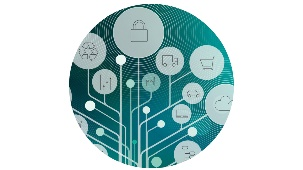
\includegraphics[width=1.33in,height=0.78in]{./media/image8.jpeg}
	\end{Center}
 \par  Research Center Data Spaces \par  www.cit.fraunhofer.de} \\
\hhline{~~~}
%row no:3
\multicolumn{1}{p{2.38in}}{} & 
\multicolumn{1}{p{1.33in}}{} & 
\multicolumn{1}{p{1.33in}}{} \\
\hhline{~~~}
%row no:4
\multicolumn{1}{p{2.38in}}{
	\begin{Center}
		
\includegraphics[width=2.38in,height=1.19in]{./media/image9.jpeg}
	\end{Center}
 \par  DEMAND \par  www.demand-projekt.de} & 
\multicolumn{1}{p{1.33in}}{} & 
\multicolumn{1}{p{1.33in}}{} \\
\hhline{~~~}

\end{tabular}
 \end{table}


%%%%%%%%%%%%%%%%%%%% Table No: 1 ends here %%%%%%%%%%%%%%%%%%%%




 %%%%%%%%%%%%  Starting New Page here %%%%%%%%%%%%%%

\newpage


\vspace{\baselineskip}
\vspace{\baselineskip}
\begin{multicols}{2}
\textbf{Authors $\&$  Contributors}\par


\vspace{\baselineskip}

\end{multicols}
\begin{itemize}
	\item Prof. Dr.-Ing. Boris Otto, Fraunhofer ISST 

	\item Sebastian Steinbuß, International Data Spaces Association 

	\item Andreas Teuscher, SICK 

	\item Dr.-Ing. Steffen Lohmann, Fraunhofer IAIS 
\end{itemize}

\vspace{\baselineskip}
\begin{multicols}{2}
\begin{itemize}
	\item Prof. Dr. Sören Auer, L3S Research Center
	\item Sebastian Bader, Fraunhofer IAIS
	\item Harrie Bastiaansen, TNO
	\item Hannes Bauer, orbiter
	\item Pascal Birnstil, Fraunhofer IOSB
	\item Martin Böhmer, Fraunhofer IML
	\item 	Dr. Jürgen Bohn, Schaeffler
	\item 	Gernot Böge, FIWARE Foundation
	\item 	Gerd Brost, Fraunhofer AISEC
	\item 	Juan Ceballos, Deutsche Telekom
	\item 	Dr.-Ing. Jan Cirullies, Fraunhofer ISST
	\item 	Constantin Ciureanu, T-Systems
	\item 	Eva Corsi, Boehringer Ingelheim
	\item 	Simon Dalmolen, TNO
	\item 	Søren Danielsen, GateHouse Logistics
	\item 	AlexanderDuisberg, Bird \& Bird
	\item 	Andreas Eitel, Fraunhofer IESE
	\item 	Thilo Ernst, Fraunhofer FOKUS
	\item 	Fabiana Fournier, IBM
	\item 	Marquart Franz, Siemens AG
	\item 	Dr. Sandra Geisler, Fraunhofer FIT
	\item 	Joshua Gelhaar, Fraunhofer ISST
	\item 	Roland Gude, Fraunhofer IAIS
	\item 	Dr.-Ing. Christian Haas, Fraunhofer IOSB
	\item 	Jürgen Heiles, Siemens
	\item 	 Burkhard Heisen, cybus
	\item 	Juanjo Hierro, FIWARE
	\item 	Joachim Hoernle, ATOS
	\item 	Manuel Huber, Fraunhofer AISEC
	\item 	Christian Jung, Fraunhofer IESE
	\item 	Prof. Dr. Jan Jürjens, Fraunhofer ISST
	\item 	Dr. Anna Kasprzik, L3S Research Center
	\item 	Dr. Markus Ketterl, msg systems
	\item 	Judith Koetzsch, Rittal
	\item 	Jacob Köhler, Deloitte
	\item 	Dr. Christoph Lange, Fraunhofer IAIS
	\item 	Dorothea Langer, Deloitte
	\item 	Jörg Langkau, nicos
	\item 	Dominik Lis, Fraunhofer ISST
	\item 	Sven Löffler, T-Systems
	\item 	Dr. Ulrich Löwen, Siemens
	\item 	Dr. Christian Mader, Fraunhofer IAIS
	\item 	Bernhard Müller, SICK
	\item 	Nadja Menz, Fraunhofer FOKUS
	\item 	Christoph Mertens, International Data Spaces Association
	\item 	Andreas Müller, Schaeffler
	\item 	Lars Nagel, International Data Spaces Association
	\item 	Dr. Ralf Nagel, Fraunhofer ISST
	\item 	Harri Nieminen, Fastems
	\item 	Thomas Reitelbach, Bosch
	\item 	Aleksei Resetko, PricewaterhouseCoopers
	\item 	Daniel Pakkala, VTT Technical Research Centre of Finland
	\item 	Florian Patzer, Fraunhofer IOSB
	\item 	Heinrich Pettenpohl, Fraunhofer ISST
	\item 	René Pietzsch, eccenca
	\item 	Jaroslav Pullmann, Fraunhofer FIT
	\item 	Matthijs Punter, TNO
	\item 	Dr. Christoph Quix, Fraunhofer FIT
	\item 	Aleksei Resetko, PwC
	\item 	Dr. Dominik Rohrmus, Siemens
	\item 	Lena Romer, Boehringer Ingelheim
	\item 	Jörg Sandlöhken, REWE Systems
	\item 	Patrick Schöwe, agma data
	\item 	Daniel Schulz, Fraunhofer IAIS
	\item 	Dr. Julian Schütte, Fraunhofer AISEC
	\item 	Dr. Karsten Schweichhart, Deutsche Telekom
	\item 	Inna Skarbowski, IBM
	\item 	Prof. Egbert-Jan Sol, TNO
	\item 	Peter Sorowka, Cybus
	\item 	Prof. Dr.-Ing. Gernot Spiegelberg, Siemens
	\item 	Markus Spiekermann, Fraunhofer ISST
	\item 	Christian Spohn, ATOS
	\item 	Gerrit Stöhr, GESIS
	\item 	Erwin Tanger, ATOS
	\item 	Dr. Michael Theß, Signal Cruncher
	\item 	Dr. Sebastian Tramp, eccenca
	\item 	Dr. Mona Wappler, thyssenkrupp
	\item 	Ann-Christin Weiergräber, Uniklinik RWTH Aachen
	\item 	Dr. Sven Wenzel, Fraunhofer ISST
	\item 	Oliver Wolff, Advaneo
	\item 	Heike Wörner, DB Schenker


\vspace{\baselineskip}

\end{itemize}
\end{multicols}


 %%%%%%%%%%%%  Starting New Page here %%%%%%%%%%%%%%

\newpage


 %%%%%%%%%%%%  This Produces Table Of Contents %%%%%%%%%%%%%%

\tableofcontents
%\addcontentsline{toc}{chapter}{Contents}



 %%%%%%%%%%%%  include section 1 Introduction here %%%%%%%%%%%%%%



\section{Introduction}\label{sec:introduction}
%\addcontentsline{toc}{section}{Introduction}
\textbf{\uppercase{The International Data Spaces (IDS) is a virtual data space leveraging existing standards and technologies, as well as governance models well-accepted in the data economy, to facilitate secure and standardized data exchange and data linkage in a trusted business ecosystem. It thereby provides a basis for creating smart-service scenarios and facilitating innovative cross-company business processes, while at the same time guaranteeing data sovereignty for data owners.}}


\subsection{Goals of the International Data Spaces}\label{subsec:Goals_of_IDS}
%\addcontentsline{toc}{subsection}{Goals of the International Data Spaces}
Data sovereignty is a central aspect of the International Data Spaces. It can be defined as a natural person’s or corporate entity’s capability of being entirely self-determined with regard to its data. The International Data Spaces initiative proposes a Reference Architecture Model for this particular capability and related aspects, including requirements for secure and trusted data exchange in business ecosystems.


Overall, there are three types of activities in which the work of the International Data Spaces initiative can be grouped: 1) research activities, 2) standardization activities, and 3) activities for the development of products and solutions for the market (see Figure \ref{fig:_Three_types_of_activities_of_the_International_Data_Spaces}): 

\begin{enumerate}
	\item The research activities are based on the first Industrial Data Space research projects conducted by Fraunhofer. They are being continued on a broad scale in a large number of projects. Each of these projects makes its own contribution to the IDS-RAM, IDS implementations, IDS use cases, and other IDS documents.

	\item  The International Data Spaces Association (IDSA), a non-profit organization, aims at promoting the IDS-RAM in order to establish an international standard. To achieve this goal, the Association pools the requirements from various industries and provides use cases to test the results gained from the model’s implementation. The standard is intended to materialize in the IDS-RAM itself, but also in defined methods for secure data exchange and data sharing facilitated by the IDS Connector, the central technical component of the International Data Spaces. To ensure the international ambition of the initiative, Regional Hubs have been established in different countries. In addition, the activities of the IDSA aim at supporting the adoption of IDS concepts and technologies in the market. 

	\item Actors in the market can make use of the International Data Spaces standard for providing software services and technology to the market. These products and solutions form the operational IDS ecosystem. As each offering must comply with the International Data Spaces standard, it must undergo a certification process. Therefore, the market requires offerings from evaluation and certification facilities.
\end{enumerate}



%%%%%%%%%%%%%%%%%%%% Figure/Image No: 3 starts here %%%%%%%%%%%%%%%%%%%%

\begin{figure}[H]
	\begin{Center}
		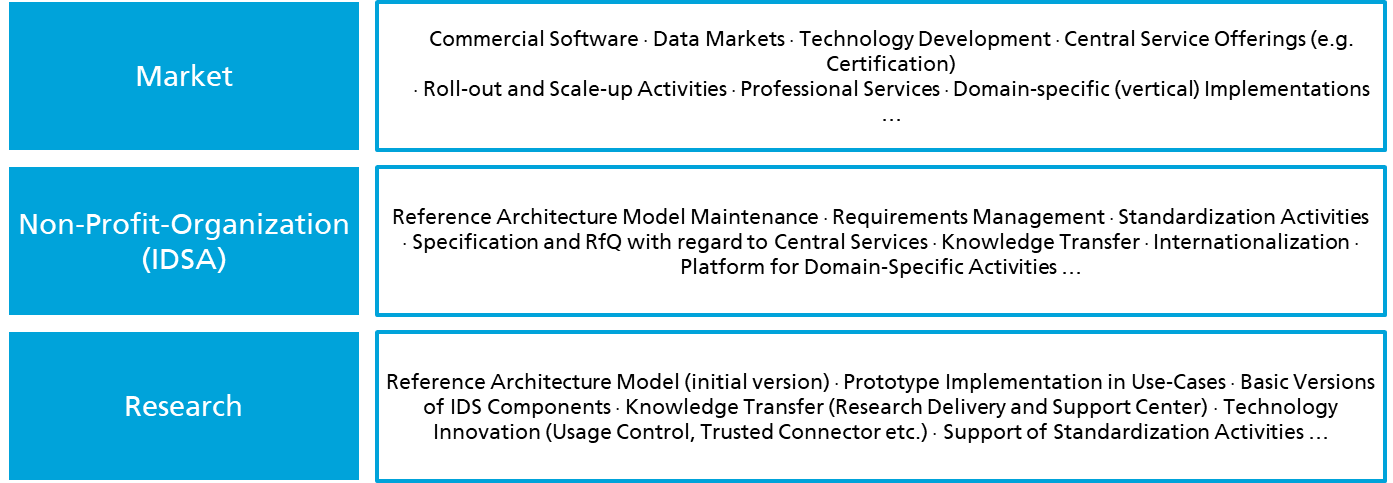
\includegraphics[width=6.35in,height=2.2in]{./media/image10.png}
		\caption{ Three types of activities of the International Data Spaces}
		\label{fig:_Three_types_of_activities_of_the_International_Data_Spaces}
	\end{Center}
\end{figure}


%%%%%%%%%%%%%%%%%%%% Figure/Image No: 3 Ends here %%%%%%%%%%%%%%%%%%%%


The International Data Spaces aims at meeting the following strategic requirements:


\begin{itemize}
	\item \textbf{Trust}: Trust is the basis of the International Data Spaces. Each participant is evaluated and certified before being granted access to the trusted business ecosystem.

	\item \textbf{Security and data sovereignty}: All components of the International Data Spaces rely on state-of-the-art security measures. Apart from architectural specifications, security is mainly ensured by the evaluation and certification of each technical component used in the International Data Spaces. In line with the central aspect of ensuring data sovereignty, a data owner in the International Data Spaces attaches usage restriction information to their data before it is transferred to a data consumer. To use the data, the data consumer must fully accept the data owner’s usage policy.

	\item \textbf{Ecosystem of data}: The architecture of the International Data Spaces does not require central data storage capabilities. Instead, it pursues the idea of decentralization of data storage, which means that data physically remains with the respective data owner until it is transferred to a trusted party. This approach requires a comprehensive description of each data source and the value and usability of data for other companies, combined with the ability to integrate domain-specific data vocabularies. In addition, brokers in the ecosystem provide services for real-time data search.

	\item \textbf{Standardized interoperability}: The International Data Spaces Connector, being a central component of the architecture, is implemented in different variants and can be acquired from different vendors. Nevertheless, each Connector is able to communicate with any other Connector (or other technical component) in the ecosystem of the International Data Space.

	\item \textbf{Value adding apps:} The International Data Spaces allows to inject apps into the IDS Connectors in order to provide services on top of data exchange processes. This includes services for data processing, data format alignment, and data exchange protocols, for example. Furthermore, data analytics services can be provided by remote execution of algorithms.

	\item \textbf{Data markets}: The International Data Space enables the creation of novel, data-driven services that make use of data apps. It also fosters new business models for these services by providing clearing mechanisms and billing functions, and by creating domain-specific broker solutions and marketplaces. In addition, the International Data Spaces provides templates and other methodological support for participants to use when specifying usage restriction information and requesting legal information. 

\end{itemize}

\textbf{Being the central deliverable of IDSA and the associated research projects associated with IDSA, the Reference Architecture Model for the International Data Spaces (IDS-RAM) constitutes the basis for a variety of software implementations, and thus for a variety of commercial software products and service offerings.}


\textbf{All research and development activities, as well as all activities with regard to standardization, are driven by the following guidelines:}

\begin{itemize}

	\item \textbf{Open development process}: The International Data Spaces Association is a non-profit organization institutionalized under the German law of associations. Every organization is invited to participate, as long as it adheres to the common principles of work.

	\item \textbf{Re-use of existing technologies}: Inter-organizational information systems, data interoperability, and information security are well-established fields of research and development, with plenty of technologies available in the market. The work of the International Data Spaces initiative is guided by the idea not to $``$reinvent the wheel$"$ , but to use existing technologies (e.g., from the open-source domain) and standards (e.g., semantic standards of the W3C) to the extent possible.

	\item \textbf{Contribution to standardization}: Aiming at establishing an international standard itself, the International Data Spaces initiative supports the idea of standardized architecture stacks.
	
	\item \textbf{Open Standard}: The IDS-RAM and the specifications associated with it are publicly available and open for being used.

\end{itemize}


\subsection{Purpose and Structure of the Reference Architecture Model}\label{subsec:purpose_of_ram}
%\addcontentsline{toc}{subsection}{Purpose and Structure of the Reference Architecture Model}
Focusing on the generalization of concepts, functionality, and overall processes involved in the creation of a secure $``$network of trusted data$"$ , the IDS-RAM resides at a higher abstraction level than common architecture models of concrete software solutions do. The document provides an overview supplemented by dedicated architecture specifications defining the individual components of the International Data Spaces (Connector, Broker, App Store, etc.) in detail.

In compliance with common system architecture models and standards (e.g., ISO 42010, 4+1 view model), the Reference Architecture Model uses a five-layer structure expressing various stakeholders’ concerns and viewpoints at different levels of granularity.

%ToDo: link sections here
The general structure of the Reference Architecture Model is illustrated in Figure \ref{fig:_General_structure_of_Reference_Architecture_Model}. The model is made up of five layers: The \textit{Business Layer} specifies and categorizes the different roles which the participants of the International Data Spaces can assume, and it specifies the main activities and interactions connected with each of these roles. The \textit{Functional Layer} defines the functional requirements of the International Data Spaces, plus the concrete features to be derived from these. The \textit{Process Layer} specifies the interactions taking place between the different components of the International Data Spaces; using the BPMN notation, it provides a dynamic view of the Reference Architecture Model. The \textit{Information Layer} defines a conceptual model which makes use of linked-data principles for describing both the static and the dynamic aspects of the International Data Space’s constituents. The \textit{System Layer} is concerned with the decomposition of the logical software components, considering aspects such as integration, configuration, deployment, and extensibility of these components.

In addition, the Reference Architecture Model comprises three perspectives that need to be implemented across all five layers: \textit{Security}, \textit{Certification}, and \textit{Governance}. 



%%%%%%%%%%%%%%%%%%%% Figure/Image No: 4 starts here %%%%%%%%%%%%%%%%%%%%

\begin{figure}[H]
	\begin{Center}
		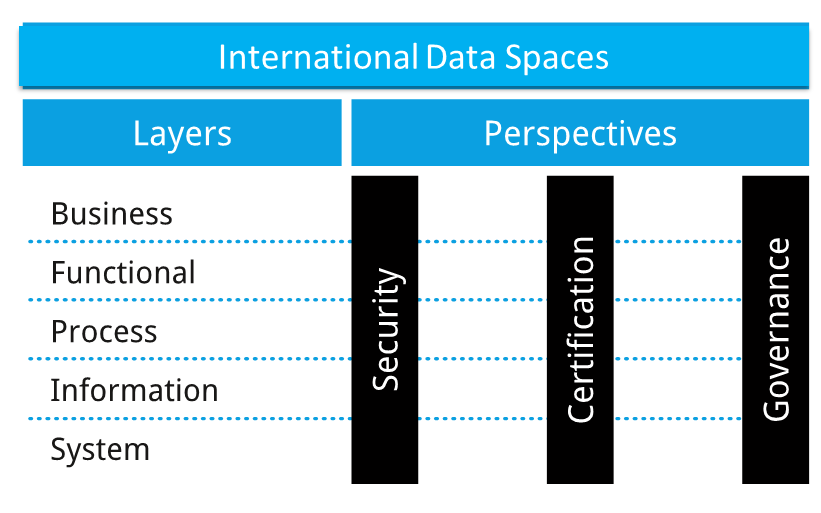
\includegraphics[width=4.12in,height=2.58in]{./media/image11.png}
		\caption{ General structure of Reference Architecture Model}
		\label{fig:_General_structure_of_Reference_Architecture_Model}
	\end{Center}
\end{figure}


%%%%%%%%%%%%%%%%%%%% Figure/Image No: 4 Ends here %%%%%%%%%%%%%%%%%%%%




 %%%%%%%%%%%%  include section 2 Context of IDS here %%%%%%%%%%%%%%

\section{Context of the International Data Spaces}\label{sec:context}
%\addcontentsline{toc}{section}{Context of the International Data Spaces}
\subsection{Data-Driven Business Ecosystems and the Smart Service Welt}\label{subsec:data_driven_business_ecosystems}
%\addcontentsline{toc}{subsection}{Data-Driven Business Ecosystems and the Smart Service Welt}
Novel digital products and services often emerge in business ecosystems, which organizations enter to jointly fulfill the needs of customers better than they can do on their own. In such ecosystems, which emerge and dissolve much faster than traditional value creating networks, the partners have a clear focus on end-to-end customer processes in order to jointly develop innovative products and services. Actors in such ecosystems can be businesses (also direct competitors), research organizations, intermediaries (electronic marketplaces, for example), governmental agencies, and customers.

Ecosystems are characterized by the fact that no member is capable of creating innovation on its own. Instead, the ecosystem as a whole needs to team up. In other words: Every member has to contribute something for the benefit of all. Ideally, ecosystems function in an equilibrium state of mutual benefits for all members.

Examples of business ecosystems are numerous and can be found across all industries. Many of them have been analyzed and documented by the Smart Service Welt working group\footnote{ https://www.digitale-technologien.de/DT/Redaktion/DE/Downloads/Publikation/SSWII\_Programmbroschuere.pdf }.
%ToDo: update reference?

A data-driven business ecosystem is an ecosystem in which data is the strategic resource used by the members to jointly create innovative value offerings. Key to success is to share and jointly maintain data within such an ecosystem, as end-to-end customer process support can only be achieved if the partners team up and jointly utilize their data resource (as shown by a number of examples in Figure \ref{fig:_Data-Driven_Business_Ecosystems_examples}).


%%%%%%%%%%%%%%%%%%%% Figure/Image No: 5 starts here %%%%%%%%%%%%%%%%%%%%

\begin{figure}[H]
	\begin{Center}
		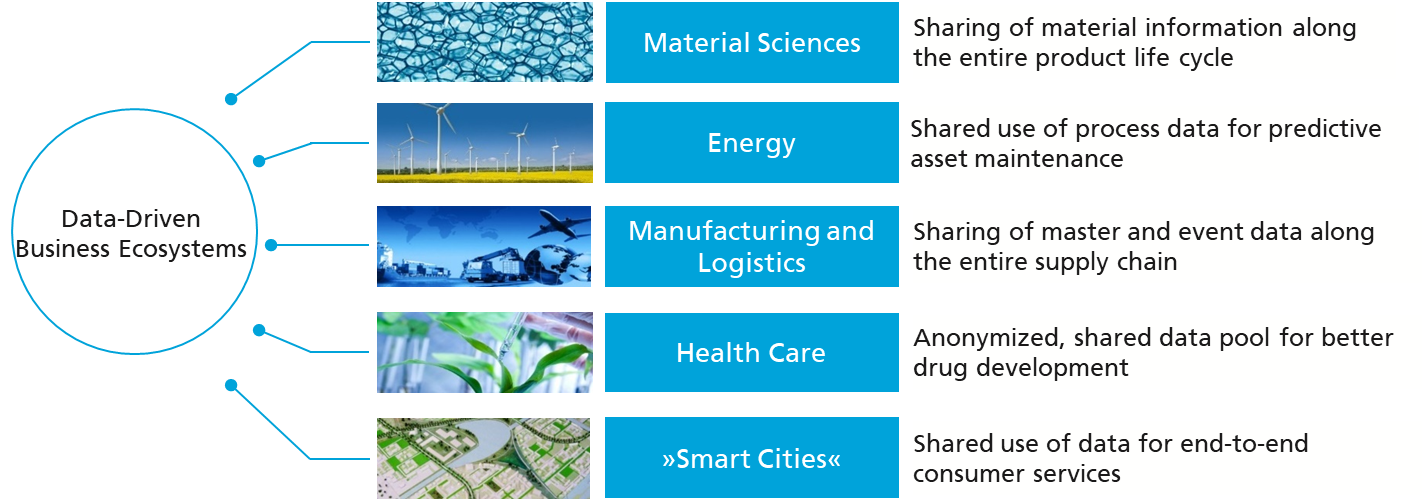
\includegraphics[width=6.42in,height=2.27in]{./media/image12.png}
		\caption{Data Sharing in Ecosystems}
		\label{fig:_Data-Driven_Business_Ecosystems_examples}
	\end{Center}
\end{figure}


%%%%%%%%%%%%%%%%%%%% Figure/Image No: 5 Ends here %%%%%%%%%%%%%%%%%%%%



\subsection{Data Sovereignty as a Key Capability}\label{subsec:datasovereignty_as_key_enabler}
%\addcontentsline{toc}{subsection}{Data Sovereignty as a Key Capability}
From these two developments – 1) data turning into a strategic resource, and 2) companies increasingly collaborating in business ecosystems – results a fundamental conflict of goals as a main characteristic of the digital economy: on the one hand, companies increasingly need to exchange data in business ecosystems; on the other hand, they feel they need to protect their data more than ever before, since the importance of data has grown so much. This conflict of goals is all the more intensified, the more a company is engaged in one or more business ecosystems, and the higher the value contributed by data to the overall success of the collaborative effort.

\textbf{Data sovereignty is about finding a balance between the need for protecting one’s data and the need for sharing one’s data with others. It can be considered a key capability for companies to develop in order to be successful in the data economy.}

To find that balance, it is important to take a close look at the data itself, as not all data requires the same level of protection, and as the value contribution of data varies, depending on what class or category it can be subsumed under.

\subsection{Data as an Economic Good}\label{subsec:data_as_economic_good}
%\addcontentsline{toc}{subsection}{Data as an Economic Good}
It is indisputable that data has a value, and that data management generates costs. Today, data is traded in the market like a commodity; it has a price, and many companies monitor the costs incurred for data management. However, data, being an intangible good, differs from tangible goods with regard to a number of properties, among which the fact that data is non-rival is considered the most important one. The value of data increases as it is being used (and, in many cases, as the number of user increases). While these differences hinder the adoption and application of legal provisions to the management and use of data, they do not dispute the fact that data is an economic good.

Depending on what type data is of, or what category it can be subsumed under, the value it contributes to the development of innovative products and services can vary. Therefore, the need for protection of data is not the same across all data types and data categories. Public data, for example, which can be accessed by anyone, requires a lower level of protection than private data or club data.

Because of these differences and distinctions made with regard to data, a generally accepted understanding of the value of data has not been established so far. Nevertheless, there is a growing need to determine the value of data, given the rapid developments taking place in the Smart Service Welt.

\subsection{Data Exchange and Data Sharing}\label{subsec:data_exchange_and_data_sharing}
%\addcontentsline{toc}{subsection}{Data Exchange and Data Sharing}
Cross-company data exchange with the help of inter-organizational information systems is not a new topic; it has been around for decades. With the proliferation of Electronic Data Interchange (EDI) in the 1980s, many different data exchange scenarios have emerged over time, which were accompanied by the development of certain technical standards.



%%%%%%%%%%%%%%%%%%%% Figure/Image No: 6 starts here %%%%%%%%%%%%%%%%%%%%

\begin{figure}[h]
	\begin{Center}
		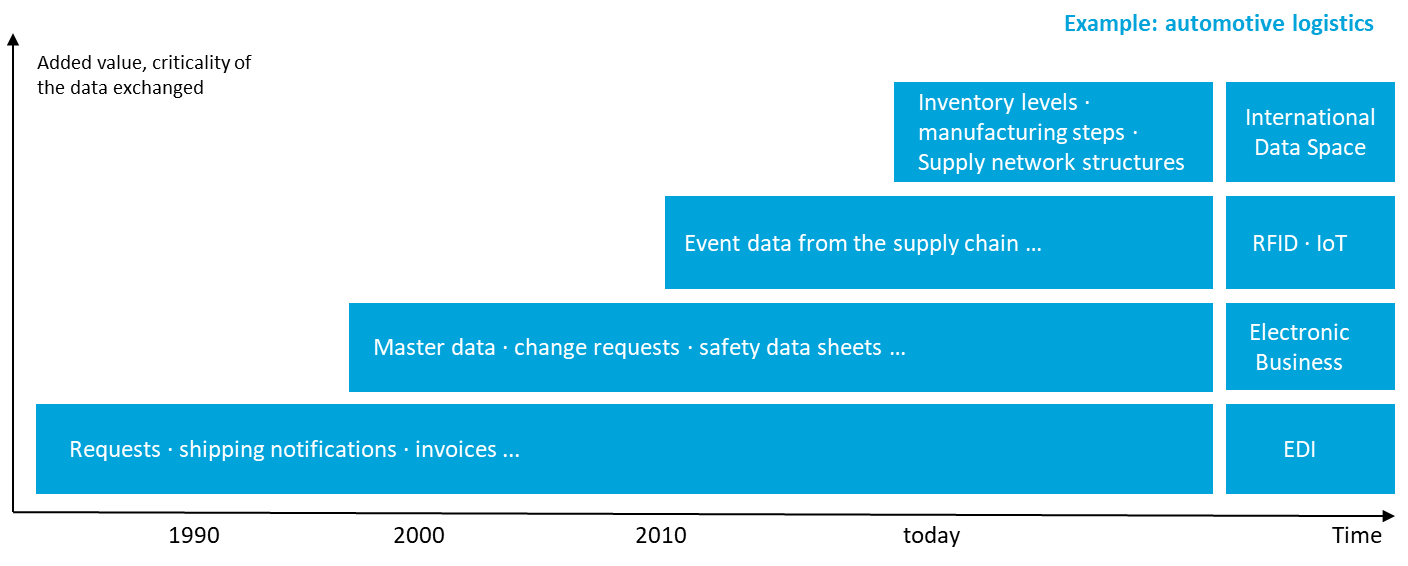
\includegraphics[width=6.67in,height=2.68in]{./media/image13.png}
		\caption{Evolution of technical standards for data exchange}
		\label{fig:Datadriven_business_ecosystems}
	\end{Center}
\end{figure}


%%%%%%%%%%%%%%%%%%%% Figure/Image No: 6 Ends here %%%%%%%%%%%%%%%%%%%%


Figure \ref{fig:Datadriven_business_ecosystems} shows the evolution of technical standards for data exchange since the 1980s, using the example of automotive logistics. Data sovereignty, which is one of the main goals of the International Data Spaces, materializes in $``$terms and conditions$"$  that are linked to data before it is exchanged and shared. However, these terms and conditions (such as time to live, forwarding rights, pricing information etc.) have not been standardized yet. In order to foster the establishment of data sovereignty in the exchange of data within business ecosystems, more standardization activities are needed.

This does not mean that existing standards will become obsolete. Instead, the overall set of standards companies need to comply with when exchanging and sharing data needs to be extended. It is therefore necessary to distinguish between data exchange and data sharing (see also Figure \ref{fig:dataexchange_vs_sharing}): 

\begin{itemize}
	\item Data exchange takes place in the \textit{vertical cooperation} between companies to support, enable or optimize value chains and supply chains (e.g. EDI messages in logistics or HL7 in medical scenarios).

	\item Data sharing takes place in the \textit{vertical and horizontal collaboration} between companies to achieve a common goal (e.g. predictive maintenance scenarios in manufacturing) or to enable new business models by generating additional value out of data (e.g. in data marketplaces). Furthermore, data sharing implies a mode of collaboration towards coopetition.

\end{itemize}



%%%%%%%%%%%%%%%%%%%% Figure/Image No: 7 starts here %%%%%%%%%%%%%%%%%%%%

\begin{figure}[H]
	\begin{Center}
		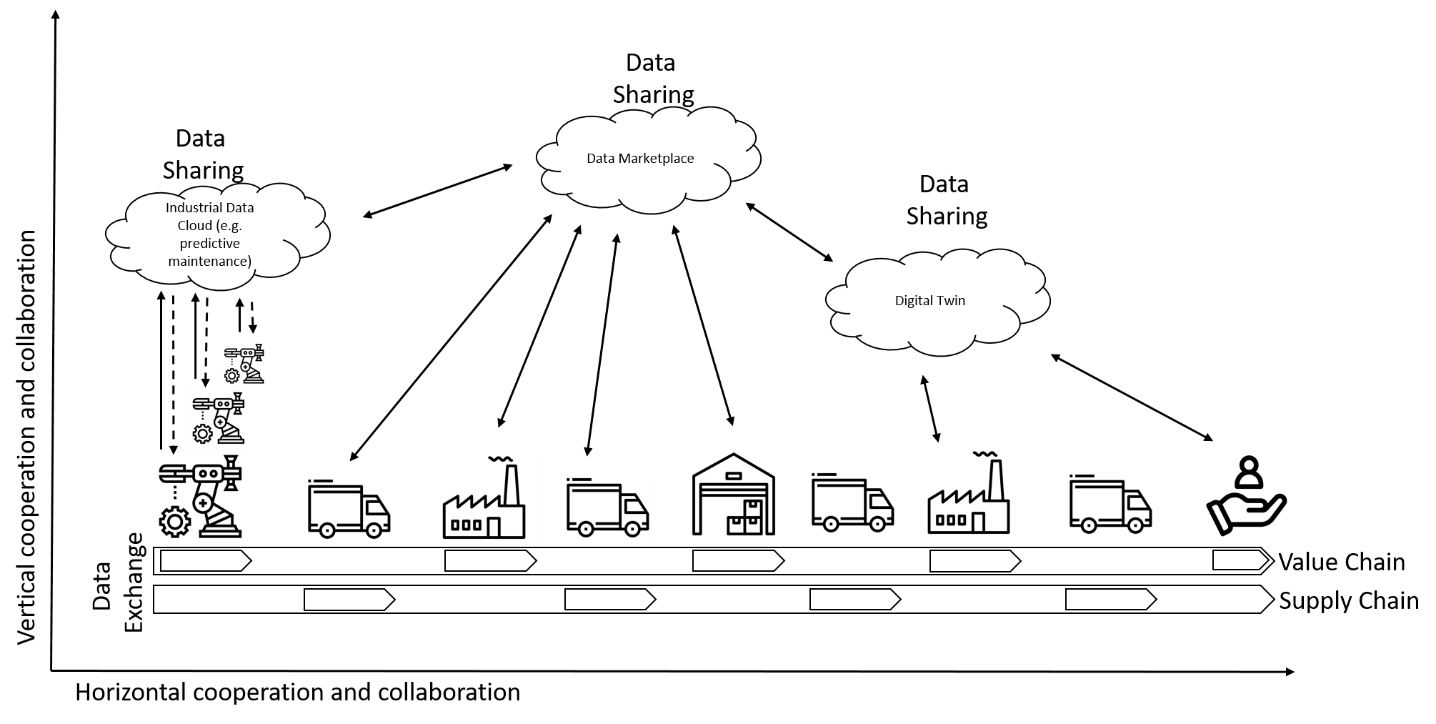
\includegraphics[width=6.53in,height=3.29in]{./media/image14.png}
		\caption{Data exchange vs. data sharing}
		\label{fig:dataexchange_vs_sharing}
	\end{Center}
\end{figure}


%%%%%%%%%%%%%%%%%%%% Figure/Image No: 7 Ends here %%%%%%%%%%%%%%%%%%%%

\subsection{Industrial Cloud Platforms}\label{subsec:industrial_cloud}
%\addcontentsline{toc}{subsection}{Industrial Cloud Platforms}
The growing number of industrial cloud platforms will also drive the need for a standard for data sovereignty. With a lot of different platforms emerging – driven by technology providers, software companies, system integrators, but also existing intermediaries – it is very likely that the platform landscape will be very heterogeneous, at least for some time. Platform providers will increasingly have to provide capabilities for secure and trusted data exchange and data sharing between their own platform and other platforms in the ecosystem.

Furthermore, the cloud platform landscape is likely to be characterized by a plurality of architectural patterns, ranging from approaches characterized by a high level of centralization (e.g. data lakes) to concepts promoting utmost decentralization (e.g. distributed applications using blockchain technology).

Which platform a data owner or data provider may choose will depend on the business criticality and the economic value of the data goods they want to exchange and share. As the data resource of a company consists of data of different criticality and value, it can be expected that many companies will use different platforms for different purposes.



%New: section on gaia x here
To make use of cloud platforms in industrial cases and to maintain data sovereignty, several preconditions must be fulfilled (especially in use cases in which different data providers bring together data in one cloud environment for being analyzed or used). The sovereign decision on a certain cloud environment must be enabled by interoperability from the perspective of data and from the perspective of the underlying software (i.e., portability of a service into different cloud environments). In addition, the capabilities of the service and the runtime must be transparent and verifiable to establish trust in the cloud environment to be used. To achieve and maintain interoperability and trust among the parties connected via a cloud environment, a governance model must be established and enforced with regard to technology, operational and administrative processes, and legal agreements.


\subsection{Big Data and Artificial Intelligence}\label{subsec:bigdata_ai}
%\addcontentsline{toc}{subsection}{Big Data and Artificial Intelligence}
Today companies make a wide use of Big Data applications. The common use case is to complement data available within the company by additional data (e.g. open data, data from other companies or data from data marketplaces). With the data portfolio extended this way, companies can benefit from significantly improved analytics results or from entirely new usage scenarios. 

Alongside with Big Data applications, also Artificial Intelligence (AI) applications have become more and more mature and powerful. Companies are increasingly using AI, which has led, and will continue to lead, to an even greater demand for external data (e.g. for training of AI models). However, companies often do not have sufficient data available in-house, which is why the need for data sharing with regard to using AI will rise.   

A standardized architecture for data exchange and data sharing would support the development and acceptance of both Big Data and AI applications in industry. At the same time, it is necessary to define usage policies for data sharing and retaining data sovereignty for data providers. 



\subsection{The Internet of Things and the Industrial Internet of Things}\label{subsec:iiot}
%\addcontentsline{toc}{subsection}{The Internet of Things and the Industrial Internet of Things}
The Internet of Things (IoT) and the Industrial Internet of Things (IIoT), respectively, comprises an ever-growing number of devices generating more and more data. While there is mostly a clear focus on the primary use of that data, it may be of interest for additional stakeholders as well. This requires standardization with regard to the (I)IoT architecture, but also standardization regarding data exchange and data sharing – in order to enable the data economy and facilitate the establishment of data marketplaces. The wide use of data generated within the (I)IoT will lead to new, smart and data centric services in conjunction with new business models.

\subsection{Blockchain}\label{subsec:blockchain}
%\addcontentsline{toc}{subsection}{Blockchain}
The core purpose of the International Data Spaces is to enable controlled exchange and sharing of data between organizations – regardless of the type of data. In many use cases of the International Data Spaces, this is some form of structured data (e.g. measurement data, product data, or logistics data). But also other types of (streaming) data are supported. The IDS Connector allows data owners and data providers to exchange and share their data with other participants in the IDS ecosystem, while data sovereignty is ensured at any time. 

In the use cases of the International Data Spaces, two basic patterns of data sharing can be found: 

\begin{itemize}
	\item Data is shared to feed new, data-driven services, such as using the data in a new app, smart algorithm, or other digital service in which data of different sources/providers is combined. 

	\item Data is shared for some form of business process synchronization, such as using the data to execute transactions (e.g. exchange orders), enable production (e.g. exchange product data), check quality (e.g. monitor the temperature of perishable goods), or synchronize processes (e.g. exchange status data). 
\end{itemize}

In many of these cases, this sharing of data enables transactions with the data itself becoming what one could call a ‘shared data asset’, resulting in liability/responsibility for the participating organizations. 

Two examples: 

\begin{itemize}
	\item As perishable goods were exposed to improper ambient temperatures, the company ordering the goods refuses acceptance. The temperature data thereby becomes a shared data asset that can be stored in a shared environment which acts as a trusted record keeper of such quality data. 

	\item Several companies want to share their capabilities in order to produce a certain type of good. In this case, the capability of each company becomes a shared data asset to be stored in shared ‘yellow pages’ accessible for all participants in the ecosystem. 
\end{itemize}

From a functional perspective, it is expected that blockchain technology will play an important role in maintaining these ‘shared data assets’ in an IDS environment. This would complement the existing capabilities of the IDS architecture to share (potentially large) datasets with the help of IDS Connectors. For instance, a shared data asset might encompass a hash code (‘fingerprint’ of a piece of data) which can be used to verify a larger file (e.g. a complex product design for which an order was sent) being shared with the help of an IDS Connector. In terms of the IDS-RAM, blockchain technology could be used for the Clearing House or the Broker, for example (see Business Layer).

In general, the use of Blockchain technology can ensure data consistency and transparency in combination with the general IDS approach for data sovereignty and secure data exchange and sharing. In contrast, typical Data Lakes focus on the integration of data for the purpose of knowledge extraction (see Figure \ref{fig:_general_architectural_patterns_for_data_exchange_and_data_sharing}).



%%%%%%%%%%%%%%%%%%%% Figure/Image No: 8 starts here %%%%%%%%%%%%%%%%%%%%

\begin{figure}[h]
	\begin{Center}
		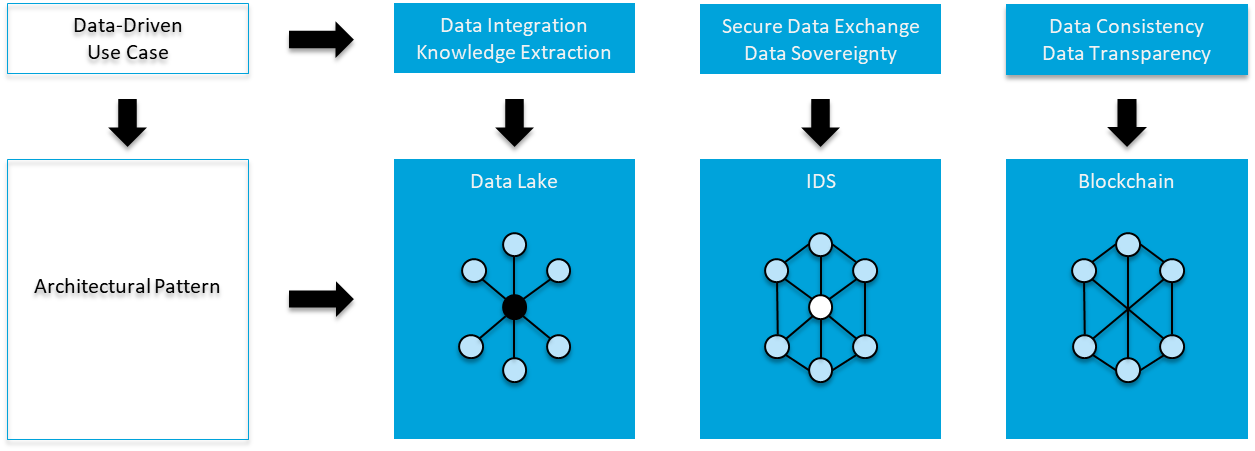
\includegraphics[width=6.6in,height=2.37in]{./media/image15.png}
		\caption{ General architectural patterns for data exchange and data sharing}
		\label{fig:_general_architectural_patterns_for_data_exchange_and_data_sharing}
	\end{Center}
\end{figure}


%%%%%%%%%%%%%%%%%%%% Figure/Image No: 8 Ends here %%%%%%%%%%%%%%%%%%%%

%new section for scheme owner
\subsection{Towards legal interoperability: federated frameworks for data sharing agreements and terms-of-use}
\label{subsection:schemeowner}

IDS provides a federated data-sharing environment that poses strong requirements with regard to interoperability on each of the levels distinguished in the new European Interoperability Framework (as developed by the European Commission ); i.e., legal, organizational, semantic and technical interoperability, under an overarching integrated governance approach.\\
Interoperability of the legal concepts applies to both the data-sharing agreements (including legal, commercial and service-level conditions) and the terms of use (i.e., usage contracts consisting of access and usage policies). In practice, different roles and organizations are currently emerging to provide services for the administration and registration of data-sharing agreements and terms of use (under the same legal umbrella, where appropriate, and specifically for certain data-sharing communities). 
Within the current IDS role and interaction model, distinct roles for managing data-sharing agreements on the one hand and terms of use on the other hand have not been specified yet. Nevertheless, supporting such roles in a federated IDS environment is key to unambiguously understanding and agreement and adequately ensuring legal compliance of data-sharing transactions taking place between parties operating in different industries, countries, and/or jurisdictions.
As a result of the co-operation between IDS and iSHARE\footnote{https://www.ishareworks.org/}, appropriate steps can be taken to address this challenge by defining the IDS approach to support federation of legal frameworks and semantic interoperability on legal conditions.
% end of new section


% new section on GDPR

\subsection{General Data Protection Regulation}
\label{subsec:gdpr}

Compliance of an organization with the European Union’s General Data Protection Regulation (GDPR) can only be ensured by the implementation of both appropriate technical and organizational measures.

For an organization participating in an IDS based ecosystem, the necessary technical measures for compliance with GDPR are provided by the software by which the IDS-RAM is implemented. However, responsibility and accountability with respect to GDPR compliance remains on the side of the organization itself. This means that the organization has to implement adequate organizational measures for the protection of personal data. This set of measures may be set up on the basis of a risk assessment regarding personal data (processing) and – if the risk level exceeds a certain threshold – a data protection impact assessment.

Consequently, the organizations participating and their data processing within an IDS-based ecosystem have to be considered for GDPR compliance. Therefore, it cannot be said in general that IDS-RAM compliance leads to GDPR compliance. Instead, the role of IDS with regard to GDPR compliance is to support the participating organization in the implementation of technical measures and offer advice regarding the implementation of organizational measures. As a result, the IDS participant is enabled to implement appropriate measures for GDPR-compliant processing and transfer of personal data within the scope of the IDS technology and related features (see also: GDPR-related Requirements and Recommendations for the IDS Reference Architecture Model \footnote{https://www.internationaldataspaces.org/ressource-hub/publications-ids/}).
% end of new section



\subsection{Contribution of the International Data Spaces to Industry 4.0 and the Data Economy}\label{subsec:contribution_to_industry40}
%\addcontentsline{toc}{subsection}{Contribution of the International Data Spaces to Industry 4.0 and the Data Economy}
By proposing an architecture for secure data exchange and trusted data sharing, the International Data Spaces contributes to the design of enterprise architectures in commercial and industrial digitization scenarios. It does so by bridging the gaps between research, industrial stakeholders, political stakeholders, and standards bodies. The architecture is designed with the objective to overcome the differences between top-down approaches and bottom-up approaches. Figure \ref{fig:5_Typical_enterprise_architecture_stack} shows a typical architecture stack of the digital industrial enterprise. The International Data Spaces connects the lower-level architectures for communication and basic data services with more abstract architectures for smart data services. It therefore supports the establishment of secure data supply chains from data source to data use, while at the same time making sure data sovereignty is guaranteed for data owners.



%%%%%%%%%%%%%%%%%%%% Figure/Image No: 9 starts here %%%%%%%%%%%%%%%%%%%%

\begin{figure}[h]
	\begin{Center}
		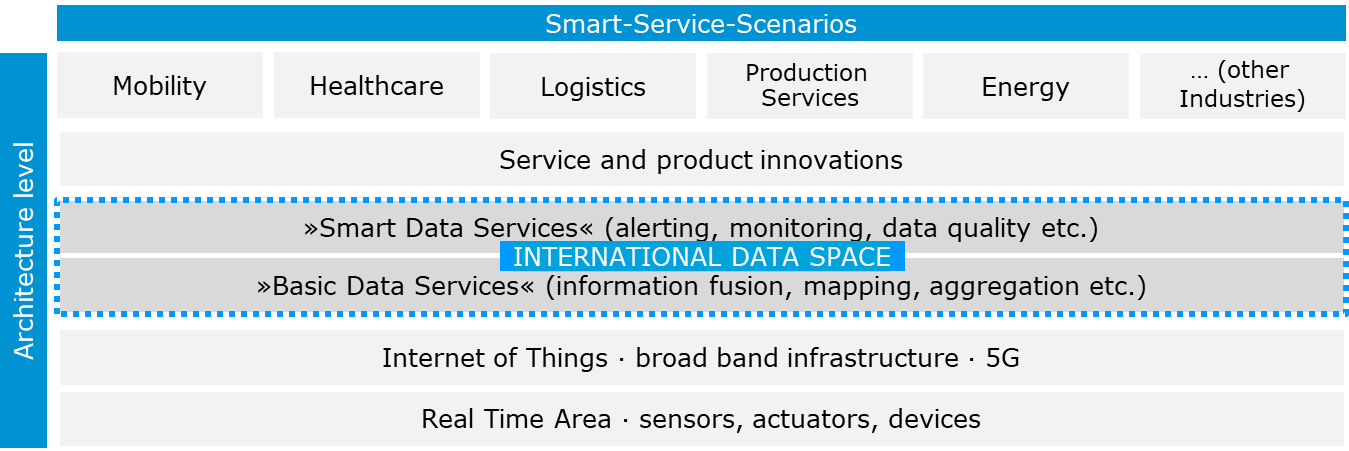
\includegraphics[width=6.25in,height=2.09in]{./media/image16.png}
		\caption{ Typical enterprise architecture stack}
		\label{fig:5_Typical_enterprise_architecture_stack}
	\end{Center}
\end{figure}


%%%%%%%%%%%%%%%%%%%% Figure/Image No: 9 Ends here %%%%%%%%%%%%%%%%%%%%



In broadening the perspective from an individual use case scenario to a platform landscape view, the International Data Spaces positions itself as an architecture that links different cloud platforms through policies and mechanisms for secure data exchange and trusted data sharing (or, in other words, through the principle of data sovereignty).\

Over the IDS Connector, the International Data Space’s central component, industrial data clouds, as well as individual enterprise clouds, on-premises applications and individual, connected devices can be connected to the International Data Spaces (see Figure \ref{fig:6_International_Data_Spaces_connecting_different_cloud_platforms}).



%%%%%%%%%%%%%%%%%%%% Figure/Image No: 10 starts here %%%%%%%%%%%%%%%%%%%%

\begin{figure}[h]
	\begin{Center}
		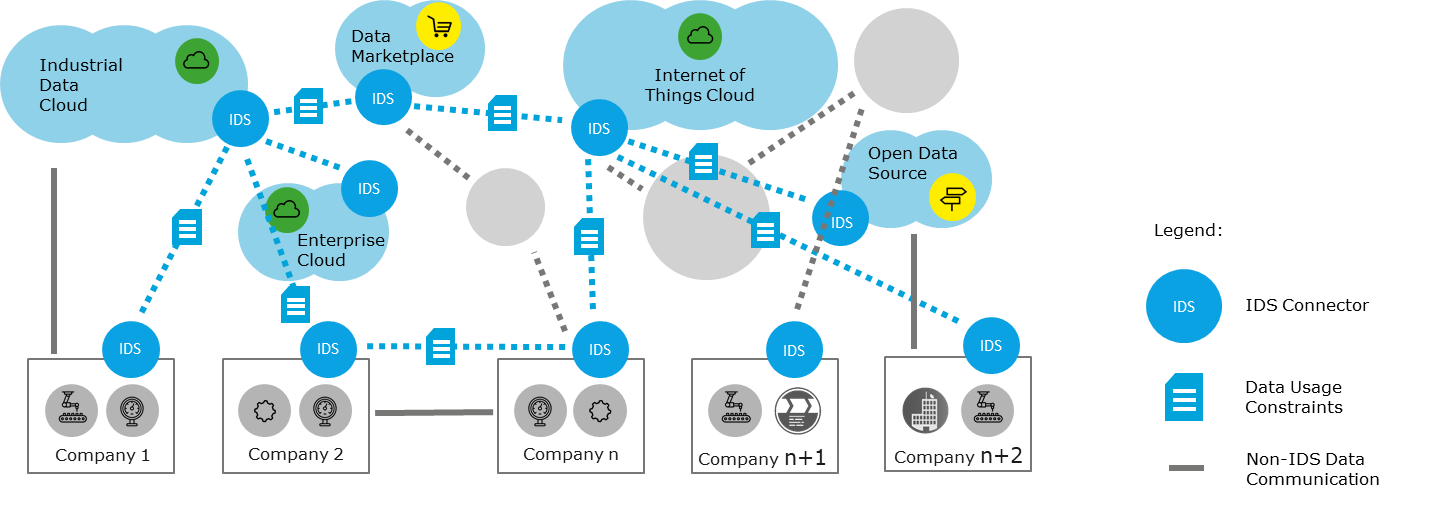
\includegraphics[width=6.42in,height=2.25in]{./media/image17.png}
		\caption{ International Data Spaces connecting different cloud platforms}
		\label{fig:6_International_Data_Spaces_connecting_different_cloud_platforms}
	\end{Center}
\end{figure}


%%%%%%%%%%%%%%%%%%%% Figure/Image No: 10 Ends here %%%%%%%%%%%%%%%%%%%%

With this integrating ambition, the International Data Spaces initiative positions itself in the context of cognate initiatives on both national and international level. Founded in Germany, the activities of the International Data Spaces are closely aligned with Plattform Industrie 4.0, in particular the Reference Architectures, Standards and Norms working group. 

The International Data Spaces initiative has established, and will continue to establish, liaisons with other initiatives, among them

%ToDo:update list
\begin{itemize}
	\item Alliance for Internet of Things Innovation,

	\item Big Data Value Association,

	\item Data Market Austria,

	\item Data Trading Alliance

	\item eCl@ss,

	\item FIWARE Foundation,

	\item Industrial Internet Consortium,

	\item iSHARE

	\item Industrial Valuechain Initative

	\item OPC Foundation,

	\item Plattform Industrie 4.0,

	\item Standardization Council Industrie 4.0, and

	\item World Wide Web Consortium.
\end{itemize}



Furthermore, the International Data Spaces initiative seeks collaboration and exchange of ideas with existing research and standardization initiatives. By functioning as a mediator between top-down and bottom-up approaches, bridging the gaps between research, industry, politics, and standards bodies, aligning the requirements of the economy and society, and fostering ties with other initiatives, the International Data Spaces can be considered a unique initiative in the landscape of \textit{Industry 4.0}.


 %%%%%%%%%%%%  include section 3 and 3.1 Business Layer here %%%%%%%%%%%%%%

\section{Layers of the Reference Architecture Model}\label{sec:layers}
The five layers of the Reference Architecture Model are presented in detail in the following subsections.

\subsection{Business Layer}\label{subsec:business_layer}
%\addcontentsline{toc}{subsection}{Business Layer}
The Business Layer of the Reference Architecture Model defines and categorizes the different roles the participants in the International Data Spaces may assume. Furthermore, it specifies basic patterns of interaction taking place between these roles. It thereby contributes to the development of innovative business models and digital, data-driven services to be used by the participants in the International Data Spaces. 

While the Business Layer provides an abstract description of the roles in the International Data Spaces, it can be considered a blueprint for the other, more technical layers. The Business Layer can therefore be used to verify the technical architecture of the International Data Spaces. In this sense, the Business Layer specifies the requirements to be addressed by the Functional Layer (see section \ref{sec_functional_layer}). 

%ToDo:update subsection
\subsubsection{Roles in the International Data Spaces}
%\addcontentsline{toc}{subsubsection}{Roles in the International Data Spaces}
In the following, each role a participant can assume in the International Data Spaces is described in detail, together with the basic tasks assigned to it. The majority of roles require certification of the organization that wants to assume that role, including certification of the technical, physical, and organizational security mechanisms the organization employs. Certification of organizations that want to participate in the International Data Spaces is considered a fundamental measure to establish trust among all participants (especially with regard to roles that are crucial for the overall functioning of the International Data Spaces, such as the Broker Service Provider, the App Store Provider, the Identity Provider, or the Clearing House). The Certification Scheme applied in the participant evaluation process is described in detail in Section 4.2.
%ToDo: refer to sec 4.2

There are four categories of roles:

\begin{itemize}
	\item Category 1: Core Participant

	\item Category 2: Intermediary

	\item Category 3: Software / Service Provider

	\item Category 4: Governance Body
\end{itemize}\par



\paragraph{Category 1: Core Participant}
Core Participants are involved and required every time data is exchanged in the International Data Spaces. Roles assigned to this category are Data Owner, Data Provider, Data Consumer, Data User, and App Provider. The role of a Core Participant can be assumed by any organization that owns, wants to provide, and/or wants to consume or use data.
\todo{CQ: Wie/Warum ist der App Provider hier reingekommen? Der ist doch für einen Datenaustausch nicht notwendig}

Benefit for participants in the International Data Spaces is created by these roles as they make data available (Data Owner), provide data (Data Provider), or consume/use data (Data Consumer, Data User, App Provider). In addition, Data Providers and Data Consumers may apply business models (including pricing models) as deemed appropriate.

\paragraph{Data Owner} %ToDo: refer to section 4.3.4
As the legal situation regarding data ownership is very complicated (as discussed in section 4.3.4), the term ‘Data Owner’ is not used in a legal understanding in this document. The Reference Architecture Model takes an operational data management perspective, defining a Data Owner as a legal entity or natural person creating data and/or executing control over it. This enables the Data Owner to define Data Usage Policies and provide access to its data. Data Ownership includes at least two major concepts:

\begin{itemize}
	\item having the (technical) means and the responsibility to define Usage Contracts and Usage Policies, and to provide access to data; and 

	\item having the (technical) means and the responsibility to define the Payment Model, including the model for reuse of data by third parties. 
\end{itemize}

Usually, a participant acting as Data Owner automatically assumes the role of the Data Provider as well. However, there may be cases in which the Data Provider is not the Data Owner (e.g., if the data is technically managed by a different entity than the Data Owner, such as in the case of a company using an external IT service provider for data management, or if data management activities are handed over to a data trustee).

In cases in which the Data Owner does not act as the Data Provider at the same time, the only activity of the Data Owner is to authorize a Data Provider to make its data available to be used by a Data Consumer. Any such authorization should be documented by a contract, which should include data usage policy information for the data provided (see. Section 4.1.3.6). The contract needs not necessarily be a paper document, but may be an electronic file as well.
%ToDo: refer to section 4.1.3.6

\paragraph{Data Provider}
The Data Provider makes data available for being exchanged between a Data Owner and a Data Consumer. As already mentioned above, the Data Provider is in most cases identical with the Data Owner, but not necessarily. To submit metadata to a Broker, or exchange data with a Data Consumer, the Data Provider uses software components that are compliant with the Reference Architecture Model of the International Data Spaces.

Providing a Data Consumer with data from a Data Owner is the main activity of the Data Provider. To facilitate a data request from a Data Consumer, the Data Provider should provide a Broker Service Provider (see below) with proper metadata about the data. However, a Broker Service Provider is not necessarily required for a Data Consumer and a Data Provider to establish a connection.

Exchanging data with a Data Consumer needs not necessarily be the only activity of the Data Provider. At the end of a data exchange transaction completely or partially executed, for example, the Data Provider may log the details of the successful (or unsuccessful) completion of the transaction at a Clearing House (see below) to facilitate billing or resolve a conflict. Furthermore, the Data Provider can use Data Apps to enrich or transform the data in some way, or to improve its quality. (Data Apps are specific applications that can be integrated into the data exchange workflow between two or more participants in the International Data Spaces.)

If the technical infrastructure for participating in the International Data Spaces is not deployed by the Data Consumer, a Data Provider may use a Service Provider (see below) to connect to the International Data Spaces.

\paragraph{Data Consumer}
The Data Consumer receives data from a Data Provider. From a business process modeling perspective, the Data Consumer is the mirror entity of the Data Provider; the activities performed by the Data Consumer are therefore similar to the activities performed by the Data Provider.

Before the connection to a Data Provider can be established, the Data Consumer can search for existing datasets by making an inquiry at a Broker Service Provider. The Broker Service Provider then provides the required metadata for the Data Consumer to connect to a Data Provider. Alternatively, the Data Consumer can establish a connection with a Data Provider directly (i.e., without involving a Broker Service Provider). In cases in which the information to connect with the Data Provider is already known to the Data Consumer, the Data Consumer may request the data (and the corresponding metadata) directly from the Data Provider.

Like a Data Provider, the Data Consumer may log the details of a successful (or unsuccessful) data exchange transaction at a Clearing House, use Data Apps to enrich, transform, etc. the data received, or use a Service Provider to connect to the International Data Spaces (if it does not deploy the technical infrastructure for participation itself).

\paragraph{Data User}
Similar to the Data Owner being the legal entity that has the legal control over its data, the Data User is the legal entity that has the legal right to use the data of a Data Owner as specified by the usage policy. In most cases, the Data User is identical with the Data Consumer. However, there may be scenarios in which these roles are assumed by different participants. For example, a patient could use a web-based software system to manage their personal health data and grant access to this data to a health coach. The data could be received from a hospital. In this case, the health coach would be the Data User and the provider of the web-based software system would be the Data Consumer.

\paragraph{App Provider} %ToDo: Refer to sec 3.5
App Providers develop Data Apps to be used in the International Data Spaces. To be deployable, a Data App has to be compliant with the system architecture of the International Data Spaces (see Section 3.5). In addition, Data Apps can be certified by a Certification Body in order to increase trust in these applications (especially with regard to Data Apps processing sensitive information). Each Data App must be published in the App Store for being accessed and used by Data Consumers and Data Providers. App Providers should describe each Data App using metadata (in compliance with a metadata model) with regard to its semantics, functionality, interfaces, etc.).


\paragraph{Category 2: Intermediary}
Intermediaries act as trusted entities. Roles assigned to this category are Broker Service Provider, Clearing House, Identity Provider, App Store Provider, and Vocabulary Provider. These roles may be assumed only by trusted organizations. 

Benefit for participants in the International Data Spaces is created by these roles by establishing trust, providing metadata, and creating a business model around their services.

\paragraph{Broker Service Provider}
The Broker Service Provider is an intermediary that stores and manages information about the data sources available in the International Data Spaces. As the role of the Broker Service Provider is central but non-exclusive, multiple Broker Service Providers may be around at the same time (e.g., for different application domains). An organization offering broker services in the International Data Spaces may assume other intermediary roles at the same time (e.g., Clearing House or Identity Provider, see below). Nevertheless, it is important to distinguish organizations and roles (e.g., assuming the role of a Broker Service Provider means that an organization deals only with metadata management; at the same time, the same organization may assume the role of a Clearing House, for which completely different tasks are defined).

The activities of the Broker Service Provider mainly focus on receiving and providing metadata. The Broker Service Provider must provide an interface for Data Providers to send their metadata. The metadata should be stored in an internal repository for being queried by Data Consumers in a structured manner. While the core of the metadata model must be specified by the International Data Spaces (i.e., by the Information Model, see Section 3.4), a Broker Service Provider may extend the metadata model to manage additional metadata elements.
%ToDo: refer to sec 3.4
%Question by Christoph Lange: Should the “extension of the metadata model” not be the job of the Vocabulary Provider?

After the Broker Service Provider has provided the Data Consumer with the metadata about a certain Data Provider, its job is done (i.e., it is not involved in the subsequent data exchange process).


\paragraph{Clearing House}
The Clearing House is an intermediary that provides clearing and settlement services for all financial and data exchange transactions. In the International Data Spaces, clearing activities are separated from broker services, since these activities are technically different from maintaining a metadata repository. As already stated above, it might still be possible that the two roles $``$Clearing House$"$  and $``$Broker Service Provider$"$  are assumed by the same organization, as both roles require acting as a trusted intermediary between the Data Provider and the Data Consumer.

The Clearing House logs all activities performed in the course of a data exchange. After a data exchange, or parts of it, has been completed, both the Data Provider and the Data Consumer confirm the data transfer by logging the details of the transaction at the Clearing House. Based on this logging information, the transaction can then be billed. The logging information can also be used to resolve conflicts (e.g., to clarify whether a data package has been received by the Data Consumer or not). The Clearing House also provides reports on the performed (logged) transactions for billing, conflict resolution, etc.

\paragraph{Identity Provider}
The Identity Provider should offer a service to create, maintain, manage, monitor, and validate identity information of and for participants in the International Data Spaces\textit{. }This is imperative for secure operation of the International Data Spaces and to avoid unauthorized access to data. 

The Identity Provider consist of a Certification Authority (managing digital certificates for the participants of the International Data Spaces), a Dynamic Attribute Provisioning Service (DAPS, managing the dynamic attributes of the participants), and a service named Dynamic Trust Monitoring (DTM, for continuous monitoring of the security and behavior of the network. More details about identity management can be found in section 4.1. %ToDo refer to sec 4.1

\paragraph{App Store Provider}
The App Store provides Data Apps. These are applications that can be deployed inside the Connector, the core technical component required for a participant to join the International Data Spaces. Data Apps facilitate data processing workflows. They may be certified by a Certification Body, following the certification procedures defined in Section 4.2. %ToDo: refer to sec 4.2

The App Store is responsible for managing information about Data Apps offered by App Providers (see below). The App Store should provide interfaces for publishing and retrieving Data Apps plus corresponding metadata.

\paragraph{Vocabulary Provider}
The Vocabulary Provider manages and offers vocabularies (i.e., ontologies, reference data models, or metadata elements) that can be used to annotate and describe datasets. In particular, the Vocabulary Provider provides the Information Model of the International Data Spaces, which is the basis for the description of data sources (see Section 3.4). In addition, other domain specific vocabularies can be provided. %ToDo refer

\paragraph{Category 3: Software / Service Provider}
This category comprises IT companies providing software and/or services (e.g., based on a software-as-a-service model) to the participants of the International Data Spaces. Roles subsumed under this category are Service Provider and Software Provider.

Benefit is created by these roles by providing software and services to the participants of the International Data Spaces. 

It should be noted that the process of providing software to be used for establishing the endpoints of a data exchange transaction (e.g. Enterprise Systems like ERP or MES, or other platforms) is not part of the International Data Spaces, as it takes place before an organization joins the IDS.



\paragraph{Service Provider}
If a participant does not deploy the technical infrastructure required for participation in the International Data Spaces itself, it may transfer the data to be made available in the International Data Spaces to a Service Provider hosting the required infrastructure for other organizations.

This role includes also providers offering additional data services (e.g., for data analysis, data integration, data cleansing, or semantic enrichment) to improve the quality of the data exchanged in the International Data Spaces. From a technical point of view, such a Service Provider can be considered a Data Provider and a Data Consumer at the same time (e.g., as a Data Consumer, it receives data from a Data Provider, then provides its specific service, and then turns into a Data Provider itself and offers the data in the International Data Spaces). 

Unlike the services provided by a Service Provider, Data Apps can be installed in the IT environment of a Data Consumer or Data Provider for implementing additional data processing functionality. To use the functionality of a Data App, the data therefore does not have to be transferred to an external Service Provider.

\paragraph{Software Provider}
A Software Provider provides software for implementing the functionality required by the International Data Spaces (i.e., through software components, as described in Section 3.5). Unlike Data Apps, software is not provided by the App Store, but delivered over the Software Providers’ usual distribution channels, and used on the basis of individual agreements between the Software Provider and the user (e.g., a Data Consumer, a Data Provider, or a Broker Service Provider). This procedure implies that the agreements between Software Providers and Data Consumers, Data Providers, etc. remain outside the scope of the International Data Spaces.

\paragraph{Category 4: Governance Body}
The Certification Body, Evaluation Facilities, and the International Data Spaces Association are the Governance Bodies of the International Data Spaces.

Benefit for participants in the International Data Spaces is created by the Certification Body and the Evaluation Facilities by taking care of the certification process and issuing certificates (both with regard to organizations that want to participate and with regard to software components that are to be used).

\paragraph{Certification Body and Evaluation Facilities}
The Certification Body, together with selected Evaluation Facilities, is in charge of the certification of the participants and the core technical components in the International Data Spaces. These Governance Bodies make sure that only compliant organizations are granted access to the trusted business ecosystem.  In this process, the Certification Body supervises the actions and decisions of the Evaluation Facilities. 

The Certification Scheme applied in the process is described in Section 4.2. %ToDO refer to sec 4.2

\paragraph{International Data Spaces Association (IDSA)}
The International Data Spaces Association (IDSA) is a non-profit organization promoting the continuous development of the International Data Spaces. More specifically, it supports and governs the continuous development of the Reference Architecture Model and the participant certification process. The International Data Spaces Association is currently organized across several working groups, each one addressing a specific topic (e.g., architecture, use cases and requirements, or certification). Members of the Association are primarily large industrial enterprises, IT companies, SMEs, research institutions, and industry associations.

As the International Data Spaces Association is not directly involved in the data exchange activities of the International Data Spaces, its role will not be further addressed in the sections on the other Layers.


\subsubsection*{Interaction of Roles }
%\addcontentsline{toc}{subsubsection}{Interaction of Roles }
\paragraph{Basic interactions for data exchange and data sharing in the International Data Spaces}
Figure \ref{fig:_Roles_and_interactions_in_the_International_Data_Spaces} gives an overview of the roles and the interactions taking place between them. As some of the roles (Certification Body and Evaluation Facilities) are not actively involved in the everyday operations of the International Data Spaces, they are omitted from the illustration. Also, the figure does not include Software Providers and Identity Providers, because of the necessary connection of those roles with all other roles. The Software Provider would be connected to all other roles with the relation $``$provides software$"$ . Likewise, the Identity Provider would be connected to all other roles with the relation $``$provides identity$"$ .

Figure \ref{fig:_Roles_and_interactions_in_the_International_Data_Spaces} shows only the basic interactions taking place between the different roles in the International Data Spaces. For data exchange, additional, more specific interactions are necessary. These interactions are described in the Process Layer section of the Reference Architecture Model (see section 3.3). %ToDo: refer to sec 3.3.

Table \ref{tab:interactions} gives an overview of possible (mandatory or optional) interactions taking place in the IDS. 



%%%%%%%%%%%%%%%%%%%% Table No: 2 starts here %%%%%%%%%%%%%%%%%%%%


\begin{table}[H]
 			\centering
\begin{tabular}{p{1.03in}p{0.22in}p{0.22in}p{0.22in}p{0.13in}p{0.13in}p{0.22in}p{0.59in}p{0.22in}p{0.2in}p{0.2in}p{0.13in}p{0.06in}p{0.13in}}
\hline
%row no:1
\multicolumn{1}{|p{1.03in}}{\cellcolor[HTML]{EFEFEF}} & 
\multicolumn{1}{|p{0.22in}}{\cellcolor[HTML]{EFEFEF}{\fontsize{9pt}{10.8pt}\selectfont \textbf{Data Owner}}} & 
\multicolumn{1}{|p{0.22in}}{\cellcolor[HTML]{EFEFEF}{\fontsize{9pt}{10.8pt}\selectfont \textbf{Data Provider}}} & 
\multicolumn{1}{|p{0.22in}}{\cellcolor[HTML]{EFEFEF}{\fontsize{9pt}{10.8pt}\selectfont \textbf{Data consumer}}} & 
\multicolumn{1}{|p{0.13in}}{\cellcolor[HTML]{EFEFEF}{\fontsize{9pt}{10.8pt}\selectfont \textbf{Data User}}} & 
\multicolumn{1}{|p{0.13in}}{\cellcolor[HTML]{EFEFEF}{\fontsize{9pt}{10.8pt}\selectfont \textbf{Broker}}} & 
\multicolumn{1}{|p{0.22in}}{\cellcolor[HTML]{EFEFEF}{\fontsize{9pt}{10.8pt}\selectfont \textbf{Clearing House}}} & 
\multicolumn{1}{|p{0.59in}}{\cellcolor[HTML]{EFEFEF}{\fontsize{9pt}{10.8pt}\selectfont \textbf{Identity Provider}}} & 
\multicolumn{1}{|p{0.22in}}{\cellcolor[HTML]{EFEFEF}{\fontsize{9pt}{10.8pt}\selectfont \textbf{Service Provider}}} & 
\multicolumn{1}{|p{0.2in}}{\cellcolor[HTML]{EFEFEF}{\fontsize{9pt}{10.8pt}\selectfont \textbf{App Provider}}} & 
\multicolumn{1}{|p{0.2in}}{\cellcolor[HTML]{EFEFEF}{\fontsize{9pt}{10.8pt}\selectfont \textbf{App Store Provider}}} & 
\multicolumn{1}{|p{0.13in}}{\cellcolor[HTML]{EFEFEF}{\fontsize{9pt}{10.8pt}\selectfont \textbf{Vocabulary Provider}}} & 
\multicolumn{1}{|p{0.06in}}{\cellcolor[HTML]{EFEFEF}{\fontsize{9pt}{10.8pt}\selectfont \textbf{Certification Body}}} & 
\multicolumn{1}{|p{0.13in}|}{\cellcolor[HTML]{EFEFEF}{\fontsize{9pt}{10.8pt}\selectfont \textbf{Evaluation Facility}}} \\
\hhline{--------------}
%row no:2
\multicolumn{1}{|p{1.03in}}{{\fontsize{11pt}{13.2pt}\selectfont Data Owner}} & 
\multicolumn{1}{|p{0.22in}}{\Centering {\fontsize{11pt}{13.2pt}\selectfont -}} & 
\multicolumn{1}{|p{0.22in}}{\Centering {\fontsize{11pt}{13.2pt}\selectfont X}} & 
\multicolumn{1}{|p{0.22in}}{\Centering {\fontsize{11pt}{13.2pt}\selectfont -}} & 
\multicolumn{1}{|p{0.13in}}{\Centering {\fontsize{11pt}{13.2pt}\selectfont -}} & 
\multicolumn{1}{|p{0.13in}}{\Centering {\fontsize{11pt}{13.2pt}\selectfont -}} & 
\multicolumn{1}{|p{0.22in}}{\Centering {\fontsize{11pt}{13.2pt}\selectfont (X)}} & 
\multicolumn{1}{|p{0.59in}}{\Centering {\fontsize{11pt}{13.2pt}\selectfont -}} & 
\multicolumn{1}{|p{0.22in}}{\Centering {\fontsize{11pt}{13.2pt}\selectfont (X)}} & 
\multicolumn{1}{|p{0.2in}}{\Centering {\fontsize{11pt}{13.2pt}\selectfont (X)}} & 
\multicolumn{1}{|p{0.2in}}{\Centering {\fontsize{11pt}{13.2pt}\selectfont (X)}} & 
\multicolumn{1}{|p{0.13in}}{\Centering {\fontsize{11pt}{13.2pt}\selectfont (X)}} & 
\multicolumn{1}{|p{0.06in}}{\Centering {\fontsize{11pt}{13.2pt}\selectfont -}} & 
\multicolumn{1}{|p{0.13in}|}{\Centering {\fontsize{11pt}{13.2pt}\selectfont (X)}} \\
\hhline{--------------}
%row no:3
\multicolumn{1}{|p{1.03in}}{{\fontsize{11pt}{13.2pt}\selectfont Data Provider}} & 
\multicolumn{1}{|p{0.22in}}{\Centering {\fontsize{11pt}{13.2pt}\selectfont X}} & 
\multicolumn{1}{|p{0.22in}}{\Centering {\fontsize{11pt}{13.2pt}\selectfont -}} & 
\multicolumn{1}{|p{0.22in}}{\Centering {\fontsize{11pt}{13.2pt}\selectfont X}} & 
\multicolumn{1}{|p{0.13in}}{} & 
\multicolumn{1}{|p{0.13in}}{\Centering {\fontsize{11pt}{13.2pt}\selectfont X}} & 
\multicolumn{1}{|p{0.22in}}{\Centering {\fontsize{11pt}{13.2pt}\selectfont (X)}} & 
\multicolumn{1}{|p{0.59in}}{\Centering {\fontsize{11pt}{13.2pt}\selectfont X}} & 
\multicolumn{1}{|p{0.22in}}{\Centering {\fontsize{11pt}{13.2pt}\selectfont (X)}} & 
\multicolumn{1}{|p{0.2in}}{\Centering {\fontsize{11pt}{13.2pt}\selectfont (X)}} & 
\multicolumn{1}{|p{0.2in}}{\Centering {\fontsize{11pt}{13.2pt}\selectfont (X)}} & 
\multicolumn{1}{|p{0.13in}}{\Centering {\fontsize{11pt}{13.2pt}\selectfont (X)}} & 
\multicolumn{1}{|p{0.06in}}{\Centering {\fontsize{11pt}{13.2pt}\selectfont -}} & 
\multicolumn{1}{|p{0.13in}|}{\Centering {\fontsize{11pt}{13.2pt}\selectfont X}} \\
\hhline{--------------}
%row no:4
\multicolumn{1}{|p{1.03in}}{{\fontsize{11pt}{13.2pt}\selectfont Data Consumer}} & 
\multicolumn{1}{|p{0.22in}}{\Centering {\fontsize{11pt}{13.2pt}\selectfont -}} & 
\multicolumn{1}{|p{0.22in}}{\Centering {\fontsize{11pt}{13.2pt}\selectfont X}} & 
\multicolumn{1}{|p{0.22in}}{\Centering {\fontsize{11pt}{13.2pt}\selectfont -}} & 
\multicolumn{1}{|p{0.13in}}{\Centering {\fontsize{11pt}{13.2pt}\selectfont X}} & 
\multicolumn{1}{|p{0.13in}}{\Centering {\fontsize{11pt}{13.2pt}\selectfont (X)}} & 
\multicolumn{1}{|p{0.22in}}{\Centering {\fontsize{11pt}{13.2pt}\selectfont (X)}} & 
\multicolumn{1}{|p{0.59in}}{\Centering {\fontsize{11pt}{13.2pt}\selectfont X}} & 
\multicolumn{1}{|p{0.22in}}{\Centering {\fontsize{11pt}{13.2pt}\selectfont (X)}} & 
\multicolumn{1}{|p{0.2in}}{\Centering {\fontsize{11pt}{13.2pt}\selectfont (X)}} & 
\multicolumn{1}{|p{0.2in}}{\Centering {\fontsize{11pt}{13.2pt}\selectfont (X)}} & 
\multicolumn{1}{|p{0.13in}}{\Centering {\fontsize{11pt}{13.2pt}\selectfont (X)}} & 
\multicolumn{1}{|p{0.06in}}{\Centering {\fontsize{11pt}{13.2pt}\selectfont -}} & 
\multicolumn{1}{|p{0.13in}|}{\Centering {\fontsize{11pt}{13.2pt}\selectfont X}} \\
\hhline{--------------}
%row no:5
\multicolumn{1}{|p{1.03in}}{{\fontsize{11pt}{13.2pt}\selectfont Data User}} & 
\multicolumn{1}{|p{0.22in}}{\Centering {\fontsize{11pt}{13.2pt}\selectfont -}} & 
\multicolumn{1}{|p{0.22in}}{\Centering {\fontsize{11pt}{13.2pt}\selectfont -}} & 
\multicolumn{1}{|p{0.22in}}{\Centering {\fontsize{11pt}{13.2pt}\selectfont X}} & 
\multicolumn{1}{|p{0.13in}}{\Centering {\fontsize{11pt}{13.2pt}\selectfont -}} & 
\multicolumn{1}{|p{0.13in}}{\Centering {\fontsize{11pt}{13.2pt}\selectfont -}} & 
\multicolumn{1}{|p{0.22in}}{\Centering {\fontsize{11pt}{13.2pt}\selectfont (X)}} & 
\multicolumn{1}{|p{0.59in}}{\Centering {\fontsize{11pt}{13.2pt}\selectfont -}} & 
\multicolumn{1}{|p{0.22in}}{\Centering {\fontsize{11pt}{13.2pt}\selectfont (X)}} & 
\multicolumn{1}{|p{0.2in}}{\Centering {\fontsize{11pt}{13.2pt}\selectfont (X)}} & 
\multicolumn{1}{|p{0.2in}}{\Centering {\fontsize{11pt}{13.2pt}\selectfont (X)}} & 
\multicolumn{1}{|p{0.13in}}{\Centering {\fontsize{11pt}{13.2pt}\selectfont (X)}} & 
\multicolumn{1}{|p{0.06in}}{\Centering {\fontsize{11pt}{13.2pt}\selectfont -}} & 
\multicolumn{1}{|p{0.13in}|}{\Centering {\fontsize{11pt}{13.2pt}\selectfont (X)}} \\
\hhline{--------------}
%row no:6
\multicolumn{1}{|p{1.03in}}{{\fontsize{11pt}{13.2pt}\selectfont Broker }} & 
\multicolumn{1}{|p{0.22in}}{\Centering {\fontsize{11pt}{13.2pt}\selectfont -}} & 
\multicolumn{1}{|p{0.22in}}{\Centering {\fontsize{11pt}{13.2pt}\selectfont (X)}} & 
\multicolumn{1}{|p{0.22in}}{\Centering {\fontsize{11pt}{13.2pt}\selectfont (X)}} & 
\multicolumn{1}{|p{0.13in}}{\Centering {\fontsize{11pt}{13.2pt}\selectfont -}} & 
\multicolumn{1}{|p{0.13in}}{\Centering {\fontsize{11pt}{13.2pt}\selectfont -}} & 
\multicolumn{1}{|p{0.22in}}{\Centering {\fontsize{11pt}{13.2pt}\selectfont -}} & 
\multicolumn{1}{|p{0.59in}}{\Centering {\fontsize{11pt}{13.2pt}\selectfont X}} & 
\multicolumn{1}{|p{0.22in}}{\Centering {\fontsize{11pt}{13.2pt}\selectfont (X)}} & 
\multicolumn{1}{|p{0.2in}}{\Centering {\fontsize{11pt}{13.2pt}\selectfont -}} & 
\multicolumn{1}{|p{0.2in}}{\Centering {\fontsize{11pt}{13.2pt}\selectfont -}} & 
\multicolumn{1}{|p{0.13in}}{\Centering {\fontsize{11pt}{13.2pt}\selectfont ?}} & 
\multicolumn{1}{|p{0.06in}}{\Centering {\fontsize{11pt}{13.2pt}\selectfont -}} & 
\multicolumn{1}{|p{0.13in}|}{\Centering {\fontsize{11pt}{13.2pt}\selectfont X}} \\
\hhline{--------------}
%row no:7
\multicolumn{1}{|p{1.03in}}{{\fontsize{11pt}{13.2pt}\selectfont Clearing House}} & 
\multicolumn{1}{|p{0.22in}}{\Centering {\fontsize{11pt}{13.2pt}\selectfont -}} & 
\multicolumn{1}{|p{0.22in}}{\Centering {\fontsize{11pt}{13.2pt}\selectfont (X)}} & 
\multicolumn{1}{|p{0.22in}}{\Centering {\fontsize{11pt}{13.2pt}\selectfont (X)}} & 
\multicolumn{1}{|p{0.13in}}{\Centering {\fontsize{11pt}{13.2pt}\selectfont -}} & 
\multicolumn{1}{|p{0.13in}}{\Centering {\fontsize{11pt}{13.2pt}\selectfont -}} & 
\multicolumn{1}{|p{0.22in}}{\Centering {\fontsize{11pt}{13.2pt}\selectfont -}} & 
\multicolumn{1}{|p{0.59in}}{\Centering {\fontsize{11pt}{13.2pt}\selectfont (X)}} & 
\multicolumn{1}{|p{0.22in}}{\Centering {\fontsize{11pt}{13.2pt}\selectfont -}} & 
\multicolumn{1}{|p{0.2in}}{\Centering {\fontsize{11pt}{13.2pt}\selectfont (X)}} & 
\multicolumn{1}{|p{0.2in}}{\Centering {\fontsize{11pt}{13.2pt}\selectfont (X)}} & 
\multicolumn{1}{|p{0.13in}}{\Centering {\fontsize{11pt}{13.2pt}\selectfont (X)}} & 
\multicolumn{1}{|p{0.06in}}{\Centering {\fontsize{11pt}{13.2pt}\selectfont -}} & 
\multicolumn{1}{|p{0.13in}|}{\Centering {\fontsize{11pt}{13.2pt}\selectfont X}} \\
\hhline{--------------}
%row no:8
\multicolumn{1}{|p{1.03in}}{{\fontsize{11pt}{13.2pt}\selectfont Identity Provider}} & 
\multicolumn{1}{|p{0.22in}}{\Centering {\fontsize{11pt}{13.2pt}\selectfont -}} & 
\multicolumn{1}{|p{0.22in}}{\Centering {\fontsize{11pt}{13.2pt}\selectfont X}} & 
\multicolumn{1}{|p{0.22in}}{\Centering {\fontsize{11pt}{13.2pt}\selectfont X}} & 
\multicolumn{1}{|p{0.13in}}{\Centering {\fontsize{11pt}{13.2pt}\selectfont -}} & 
\multicolumn{1}{|p{0.13in}}{\Centering {\fontsize{11pt}{13.2pt}\selectfont X}} & 
\multicolumn{1}{|p{0.22in}}{\Centering {\fontsize{11pt}{13.2pt}\selectfont (X)}} & 
\multicolumn{1}{|p{0.59in}}{\Centering {\fontsize{11pt}{13.2pt}\selectfont Federation}} & 
\multicolumn{1}{|p{0.22in}}{\Centering {\fontsize{11pt}{13.2pt}\selectfont -}} & 
\multicolumn{1}{|p{0.2in}}{\Centering {\fontsize{11pt}{13.2pt}\selectfont (X)?}} & 
\multicolumn{1}{|p{0.2in}}{\Centering {\fontsize{11pt}{13.2pt}\selectfont (X)?}} & 
\multicolumn{1}{|p{0.13in}}{\Centering {\fontsize{11pt}{13.2pt}\selectfont -}} & 
\multicolumn{1}{|p{0.06in}}{\Centering {\fontsize{11pt}{13.2pt}\selectfont -}} & 
\multicolumn{1}{|p{0.13in}|}{\Centering {\fontsize{11pt}{13.2pt}\selectfont X}} \\
\hhline{--------------}
%row no:9
\multicolumn{1}{|p{1.03in}}{{\fontsize{11pt}{13.2pt}\selectfont Service Provider}} & 
\multicolumn{1}{|p{0.22in}}{\Centering {\fontsize{11pt}{13.2pt}\selectfont (X)}} & 
\multicolumn{1}{|p{0.22in}}{\Centering {\fontsize{11pt}{13.2pt}\selectfont (X)}} & 
\multicolumn{1}{|p{0.22in}}{\Centering {\fontsize{11pt}{13.2pt}\selectfont (X)}} & 
\multicolumn{1}{|p{0.13in}}{\Centering {\fontsize{11pt}{13.2pt}\selectfont (X)}} & 
\multicolumn{1}{|p{0.13in}}{\Centering {\fontsize{11pt}{13.2pt}\selectfont (X)}} & 
\multicolumn{1}{|p{0.22in}}{\Centering {\fontsize{11pt}{13.2pt}\selectfont -}} & 
\multicolumn{1}{|p{0.59in}}{\Centering {\fontsize{11pt}{13.2pt}\selectfont -}} & 
\multicolumn{1}{|p{0.22in}}{\Centering {\fontsize{11pt}{13.2pt}\selectfont -}} & 
\multicolumn{1}{|p{0.2in}}{\Centering {\fontsize{11pt}{13.2pt}\selectfont (X)}} & 
\multicolumn{1}{|p{0.2in}}{\Centering {\fontsize{11pt}{13.2pt}\selectfont (X)}} & 
\multicolumn{1}{|p{0.13in}}{\Centering {\fontsize{11pt}{13.2pt}\selectfont (X)}} & 
\multicolumn{1}{|p{0.06in}}{\Centering {\fontsize{11pt}{13.2pt}\selectfont -}} & 
\multicolumn{1}{|p{0.13in}|}{\Centering {\fontsize{11pt}{13.2pt}\selectfont X}} \\
\hhline{--------------}
%row no:10
\multicolumn{1}{|p{1.03in}}{{ Vocabulary Provider}} & 
\multicolumn{1}{|p{0.22in}}{\Centering {\fontsize{11pt}{13.2pt}\selectfont (X)}} & 
\multicolumn{1}{|p{0.22in}}{\Centering {\fontsize{11pt}{13.2pt}\selectfont (X)}} & 
\multicolumn{1}{|p{0.22in}}{\Centering {\fontsize{11pt}{13.2pt}\selectfont (X)}} & 
\multicolumn{1}{|p{0.13in}}{\Centering {\fontsize{11pt}{13.2pt}\selectfont (X)}} & 
\multicolumn{1}{|p{0.13in}}{\Centering {\fontsize{11pt}{13.2pt}\selectfont ?}} & 
\multicolumn{1}{|p{0.22in}}{\Centering {\fontsize{11pt}{13.2pt}\selectfont (X)}} & 
\multicolumn{1}{|p{0.59in}}{\Centering {\fontsize{11pt}{13.2pt}\selectfont -}} & 
\multicolumn{1}{|p{0.22in}}{\Centering {\fontsize{11pt}{13.2pt}\selectfont (X)}} & 
\multicolumn{1}{|p{0.2in}}{\Centering {\fontsize{11pt}{13.2pt}\selectfont (X)}} & 
\multicolumn{1}{|p{0.2in}}{\Centering {\fontsize{11pt}{13.2pt}\selectfont (X)}} & 
\multicolumn{1}{|p{0.13in}}{\Centering {\fontsize{11pt}{13.2pt}\selectfont -}} & 
\multicolumn{1}{|p{0.06in}}{\Centering {\fontsize{11pt}{13.2pt}\selectfont -}} & 
\multicolumn{1}{|p{0.13in}|}{\Centering {\fontsize{11pt}{13.2pt}\selectfont X}} \\
\hhline{--------------}
%row no:11
\multicolumn{1}{|p{1.03in}}{{ App Provider}} & 
\multicolumn{1}{|p{0.22in}}{\Centering {\fontsize{11pt}{13.2pt}\selectfont (X)}} & 
\multicolumn{1}{|p{0.22in}}{\Centering {\fontsize{11pt}{13.2pt}\selectfont (X)}} & 
\multicolumn{1}{|p{0.22in}}{\Centering {\fontsize{11pt}{13.2pt}\selectfont (X)}} & 
\multicolumn{1}{|p{0.13in}}{\Centering {\fontsize{11pt}{13.2pt}\selectfont (X)}} & 
\multicolumn{1}{|p{0.13in}}{\Centering {\fontsize{11pt}{13.2pt}\selectfont -}} & 
\multicolumn{1}{|p{0.22in}}{\Centering {\fontsize{11pt}{13.2pt}\selectfont (X)}} & 
\multicolumn{1}{|p{0.59in}}{\Centering {\fontsize{11pt}{13.2pt}\selectfont (X)}} & 
\multicolumn{1}{|p{0.22in}}{\Centering {\fontsize{11pt}{13.2pt}\selectfont (X)}} & 
\multicolumn{1}{|p{0.2in}}{\Centering {\fontsize{11pt}{13.2pt}\selectfont -}} & 
\multicolumn{1}{|p{0.2in}}{\Centering {\fontsize{11pt}{13.2pt}\selectfont (X)}} & 
\multicolumn{1}{|p{0.13in}}{\Centering {\fontsize{11pt}{13.2pt}\selectfont -}} & 
\multicolumn{1}{|p{0.06in}}{\Centering {\fontsize{11pt}{13.2pt}\selectfont -}} & 
\multicolumn{1}{|p{0.13in}|}{\Centering {\fontsize{11pt}{13.2pt}\selectfont (X)}} \\
\hhline{--------------}
%row no:12
\multicolumn{1}{|p{1.03in}}{{\fontsize{11pt}{13.2pt}\selectfont App Store Provider}} & 
\multicolumn{1}{|p{0.22in}}{\Centering {\fontsize{11pt}{13.2pt}\selectfont (X)}} & 
\multicolumn{1}{|p{0.22in}}{\Centering {\fontsize{11pt}{13.2pt}\selectfont (X)}} & 
\multicolumn{1}{|p{0.22in}}{\Centering {\fontsize{11pt}{13.2pt}\selectfont (X)}} & 
\multicolumn{1}{|p{0.13in}}{\Centering {\fontsize{11pt}{13.2pt}\selectfont (X)}} & 
\multicolumn{1}{|p{0.13in}}{\Centering {\fontsize{11pt}{13.2pt}\selectfont -}} & 
\multicolumn{1}{|p{0.22in}}{\Centering {\fontsize{11pt}{13.2pt}\selectfont (X)}} & 
\multicolumn{1}{|p{0.59in}}{\Centering {\fontsize{11pt}{13.2pt}\selectfont (X)?}} & 
\multicolumn{1}{|p{0.22in}}{\Centering {\fontsize{11pt}{13.2pt}\selectfont (X)}} & 
\multicolumn{1}{|p{0.2in}}{\Centering {\fontsize{11pt}{13.2pt}\selectfont (X)}} & 
\multicolumn{1}{|p{0.2in}}{\Centering {\fontsize{11pt}{13.2pt}\selectfont -}} & 
\multicolumn{1}{|p{0.13in}}{\Centering {\fontsize{11pt}{13.2pt}\selectfont (X)}} & 
\multicolumn{1}{|p{0.06in}}{\Centering {\fontsize{11pt}{13.2pt}\selectfont -}} & 
\multicolumn{1}{|p{0.13in}|}{\Centering {\fontsize{11pt}{13.2pt}\selectfont X}} \\
\hhline{--------------}
%row no:13
\multicolumn{1}{|p{1.03in}}{{\fontsize{11pt}{13.2pt}\selectfont Certification Body}} & 
\multicolumn{1}{|p{0.22in}}{\Centering {\fontsize{11pt}{13.2pt}\selectfont -}} & 
\multicolumn{1}{|p{0.22in}}{\Centering {\fontsize{11pt}{13.2pt}\selectfont -}} & 
\multicolumn{1}{|p{0.22in}}{\Centering {\fontsize{11pt}{13.2pt}\selectfont -}} & 
\multicolumn{1}{|p{0.13in}}{\Centering {\fontsize{11pt}{13.2pt}\selectfont -}} & 
\multicolumn{1}{|p{0.13in}}{\Centering {\fontsize{11pt}{13.2pt}\selectfont -}} & 
\multicolumn{1}{|p{0.22in}}{\Centering {\fontsize{11pt}{13.2pt}\selectfont -}} & 
\multicolumn{1}{|p{0.59in}}{\Centering {\fontsize{11pt}{13.2pt}\selectfont -}} & 
\multicolumn{1}{|p{0.22in}}{\Centering {\fontsize{11pt}{13.2pt}\selectfont -}} & 
\multicolumn{1}{|p{0.2in}}{\Centering {\fontsize{11pt}{13.2pt}\selectfont -}} & 
\multicolumn{1}{|p{0.2in}}{\Centering {\fontsize{11pt}{13.2pt}\selectfont -}} & 
\multicolumn{1}{|p{0.13in}}{\Centering {\fontsize{11pt}{13.2pt}\selectfont -}} & 
\multicolumn{1}{|p{0.06in}}{\Centering {\fontsize{11pt}{13.2pt}\selectfont -}} & 
\multicolumn{1}{|p{0.13in}|}{\Centering {\fontsize{11pt}{13.2pt}\selectfont X}} \\
\hhline{--------------}
%row no:14
\multicolumn{1}{|p{1.03in}}{{\fontsize{11pt}{13.2pt}\selectfont Evaluation Facility}} & 
\multicolumn{1}{|p{0.22in}}{\Centering {\fontsize{11pt}{13.2pt}\selectfont (X)}} & 
\multicolumn{1}{|p{0.22in}}{\Centering {\fontsize{11pt}{13.2pt}\selectfont X}} & 
\multicolumn{1}{|p{0.22in}}{\Centering {\fontsize{11pt}{13.2pt}\selectfont X}} & 
\multicolumn{1}{|p{0.13in}}{\Centering {\fontsize{11pt}{13.2pt}\selectfont (X)}} & 
\multicolumn{1}{|p{0.13in}}{\Centering {\fontsize{11pt}{13.2pt}\selectfont X}} & 
\multicolumn{1}{|p{0.22in}}{\Centering {\fontsize{11pt}{13.2pt}\selectfont X}} & 
\multicolumn{1}{|p{0.59in}}{\Centering {\fontsize{11pt}{13.2pt}\selectfont X}} & 
\multicolumn{1}{|p{0.22in}}{\Centering {\fontsize{11pt}{13.2pt}\selectfont X}} & 
\multicolumn{1}{|p{0.2in}}{\Centering {\fontsize{11pt}{13.2pt}\selectfont (X)}} & 
\multicolumn{1}{|p{0.2in}}{\Centering {\fontsize{11pt}{13.2pt}\selectfont X}} & 
\multicolumn{1}{|p{0.13in}}{\Centering {\fontsize{11pt}{13.2pt}\selectfont X}} & 
\multicolumn{1}{|p{0.06in}}{\Centering {\fontsize{11pt}{13.2pt}\selectfont X}} & 
\multicolumn{1}{|p{0.13in}|}{\Centering {\fontsize{11pt}{13.2pt}\selectfont -}} \\
\hhline{--------------}


\end{tabular}
\caption{Interactions between roles in the IDS – X --> mandatory interaction, (X) --> optional interaction}
\label{tab:interactions}
 \end{table}


%%%%%%%%%%%%%%%%%%%% Table No: 2 ends here %%%%%%%%%%%%%%%%%%%%



%%%%%%%%%%%%%%%%%%%% Figure/Image No: 11 starts here %%%%%%%%%%%%%%%%%%%%

\begin{figure}[H]
	\begin{Center}
		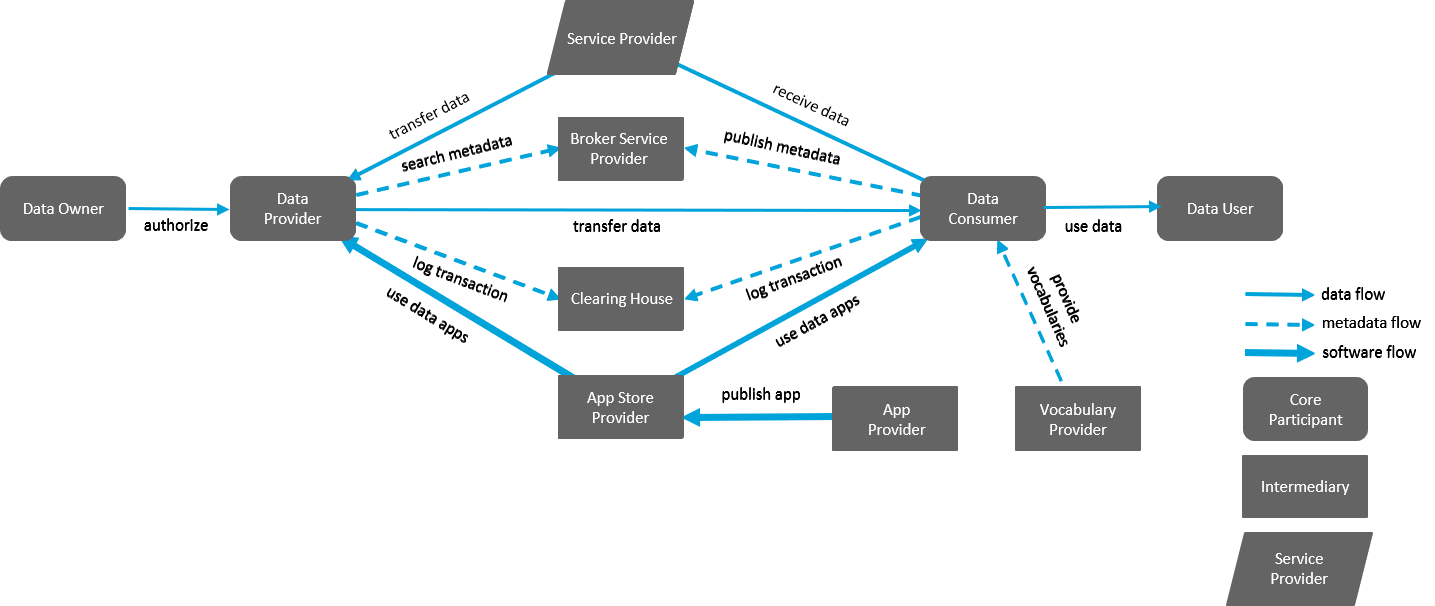
\includegraphics[width=6.53in,height=4.32in]{./media/image18.png}
		\caption{ Roles and interactions in the International Data Spaces}
		\label{fig:_Roles_and_interactions_in_the_International_Data_Spaces}
	\end{Center}
\end{figure}


%%%%%%%%%%%%%%%%%%%% Figure/Image No: 11 Ends here %%%%%%%%%%%%%%%%%%%%




\subsubsection{Digital Identities}
%\addcontentsline{toc}{subsubsection}{Digital Identities}

Establishing trust for data sharing and data exchange is a fundamental requirement. The IDS-RAM defines two basic types of trust: 1) Static Trust, based on the certification of participants and core technical components, and 2) Dynamic Trust, based on active monitoring of participants and core technical components. For data sharing and data exchange in the IDS, some preliminary actions and interactions are required. These are necessary for every participant, and involve the Certification Body, Evaluation Facilities, and the Dynamic Attribute Provisioning Service (DAPS). Figure \ref{fig:_Interactions_required_for_issuing_a_digital_identity_in_the_IDS} illustrates the roles and interactions required for issuing a digital identity in the IDS.  


%%%%%%%%%%%%%%%%%%%% Figure/Image No: 11 starts here %%%%%%%%%%%%%%%%%%%%

\begin{figure}[H]
	\begin{Center}
		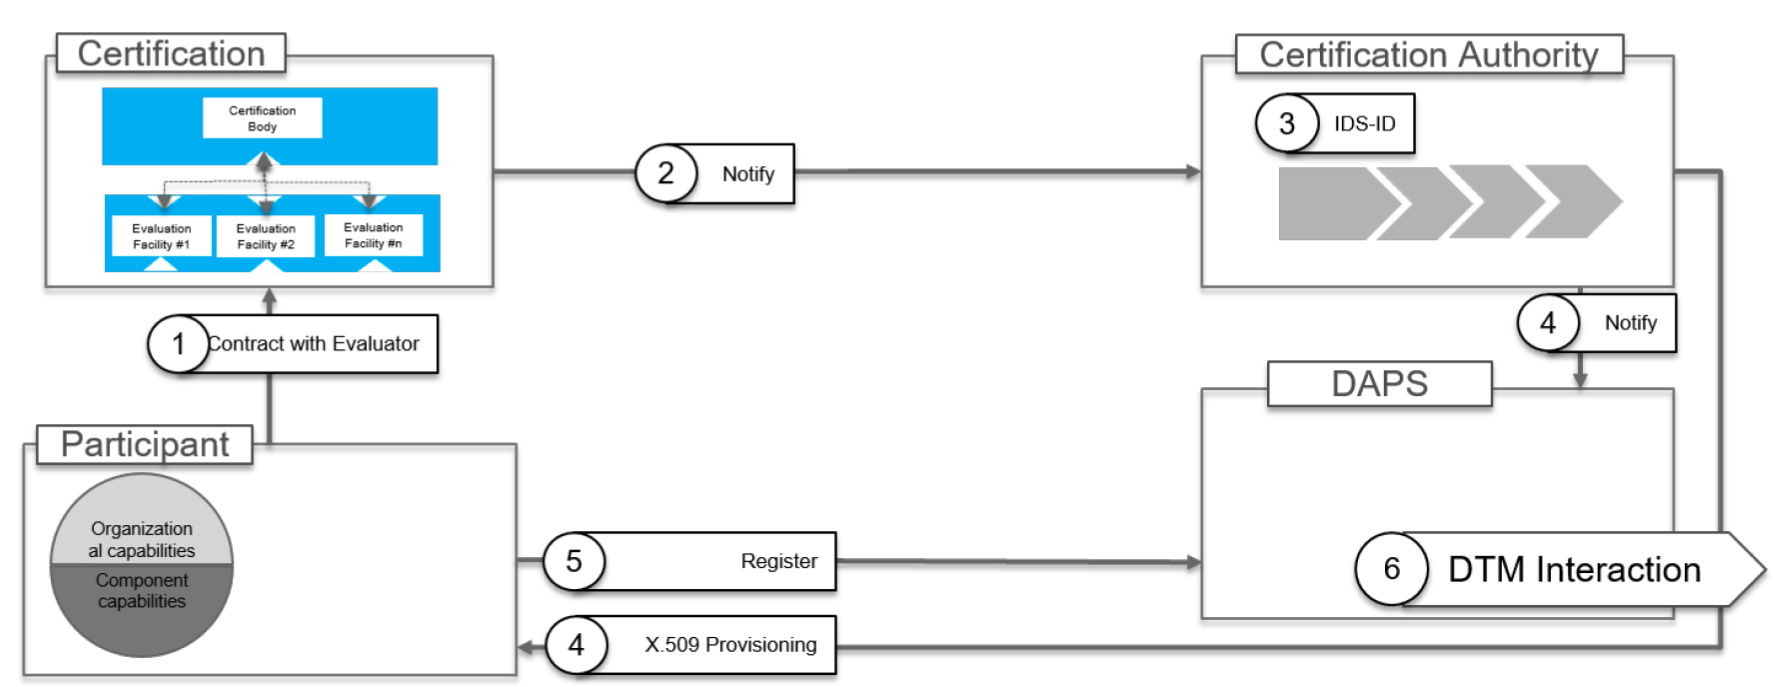
\includegraphics[width=6.53in,height=4.32in]{./media/DigitalIdentities.png}
		\caption{ Interactions required for issuing a digital identity in the IDS}
		\label{fig:_Interactions_required_for_issuing_a_digital_identity_in_the_IDS}
	\end{Center}
\end{figure}


%%%%%%%%%%%%%%%%%%%% Figure/Image No: 11 Ends here %%%%%%%%%%%%%%%%%%%%








\paragraph{Participant}
Certification is required for every participant and the majority of roles in the IDS, as defined above. Certification refers both to the organizational capabilities of the participant and the technical capabilities of the core technical components.


\paragraph{Certification} %ToDo: refer to section 4.2
Certification of a participant or core component involves the Certification Body and an Evaluation Facility (see section 4.2). Evaluation of a participant or a core component is executed upon request of the participant and relies on the contract between the participant and the Evaluation Facility. In the same way, a Service Provider can request evaluation of a component. In this process, the Certification Body is responsible for supervision of the Evaluation Facility involved.


\paragraph{Certification Authority} %ToDo: refer to sec 4.1
The Certification Authority is responsible for issuing, validating and revoking digital certificates (see section 4.1). A digital certificate is provided for a participant if both a valid certification for the participant and a valid certification for the core component is available. This means that the Certification Authority provides an IDS-ID for a combination of participant and core component. The digital certificate is valid not exceeding the validity of both certifications, participant certification and the certification of core component used by the participant. The Certification Authority provides the digital certificate to the participant upon request.


\paragraph{Dynamic Attribute Provisioning Service (DAPS)} %ToDo: referer
The information resulting from the certification process is passed on to the Dynamic Attribute Provisioning Service (DAPS). This includes master data and information on security profiles (see section 4.1.3.3.6 and Appendix B).  The CA provides the details on the digital certificate (public key and IDS-ID). The participant registers at the DAPS after successfully deploying the digital certificate inside the component.


\paragraph{Dynamic Trust Monitoring (DTM)}
Continuous monitoring of participants is necessary for classification of the trustworthiness of all participants in the ecosystem. Dynamic Trust Monitoring (DTM) implements a monitoring function for every IDS Component. The DTM shares information with the DAPS to notify each of the two participant in a data exchange transaction of the current level of trustworthiness of the other participant.


\paragraph{Interactions}
The roles described above interact with each other in a structured way, as described in Figure \ref{fig:_Interactions_required_for_issuing_a_digital_identity_in_the_IDS}. In the following, a brief description of these interactions is given (they are described in more detail in subsequent sections of the document): 


%\begin{enumerate}[label*={\fontsize{11pt}{11pt}\selectfont \arabic*.}]
\begin{enumerate}
	\item \textbf{Certification request:} This is a direct interaction between a participant and an evaluation facility to trigger an evaluation process based on IDS certification criteria.

	\item \textbf{Notification of successful certification:} The Certification Body notifies the Certification Authority of the successful certification of the participant and the core component. Validity of both certifications must be provided.

	\item \textbf{Generating the IDS-ID:} The CA generates a unique ID for the pair (participant and component) and issues a digital certificate (X.509).

	\item \textbf{Provisioning of X.509 Certificate:} The Certification Authority sends a digital certificate (X.509) to the participant in a secure and trustworthy way and notifies the DAPS.

	\item \textbf{Register:} After the digital certificate (X.509) is deployed inside the component, the component registers at the DAPS.

	\item \textbf{DTM Interaction}: The DTM and the DAPS exchange information on the behavior of the component, e.g. about security issues (vulnerabilities) or attempted attacks. 

\end{enumerate}




\subsubsection{Usage Contracts}
%\addcontentsline{toc}{subsubsection}{Usage Contracts}
A legally valid contract is the foundation of any business transaction. The IDS cannot, and does not intend to, replace legal contracts or licensing agreements. Instead, the IDS provides a technical framework for technically enforced agreements in addition to existing, legally binding contracts.

Many details of a business relationship cannot be modeled in machine-readable form. Nevertheless, the IDS specifies methods to define categories of applicable contracts, and it presents patterns to observe their usage and report validations. For this purpose, the IDS makes use of the Information Layer (see section 3.4). %ToDo:referer





%%%%%%%%%%%%%%%%%%%% Figure/Image No: 12 starts here %%%%%%%%%%%%%%%%%%%%

\begin{figure}[H]
	\begin{Center}
		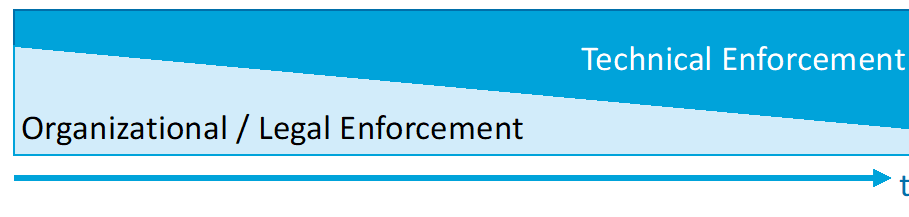
\includegraphics[width=6.53in,height=1.56in]{./media/image20_new.png}
		\caption{echnical Enforcement and organizational enforcement of usage policies}
		\label{fig:echnical_Enforcement_and_organizational_enforcement_of_usage_policies}
	\end{Center}
\end{figure}


%%%%%%%%%%%%%%%%%%%% Figure/Image No: 12 Ends here %%%%%%%%%%%%%%%%%%%%


%ToDo: referer
A Usage Contract comprises a set of Usage Policies. Each policy describes a certain permission or obligation of an IDS Resource (see section 3.4.3.2). Usage Contracts are written in a machine-readable format (according to the IDS Usage Policy Language, see section 3.4.4.1.1) and must be interpreted as defined in section 4.1.3.6. In any case, a Usage Contract must always be regarded as an extension of an existing legal agreement between two IDS participants, which can be overruled by them. As neither the IDS nor any other known technology stack can sufficiently interpret legal texts, any Usage Contract must always be in line with the concluded agreements. 
Each contract between IDS participants consists of a technical part and a non-technical part. The technical part focuses on the description of technical interfaces (Application Programming Interfaces) and the Usage Policy. Negotiation of the technical part of a contract must be supported by the Information Layer of the IDS-RAM. The non-technical part focuses on legal aspects of the intended data exchange. For automatic negotiation of contracts and conditions standard contracts are necessary (but not yet available today). 

%%%%%%%%%%%%%%%%%%

\subsection{Functional Layer}
\label{sec_functional_layer}
%\addcontentsline{toc}{subsection}{Functional Layer}
The Functional Layer defines –  irrespective of existing technologies and applications –  the functional requirements of the International Data Spaces, and the features to be implemented resulting thereof.



%%%%%%%%%%%%%%%%%%%% Figure/Image No: 13 starts here %%%%%%%%%%%%%%%%%%%%

\begin{figure}[H]
	\begin{Center}
		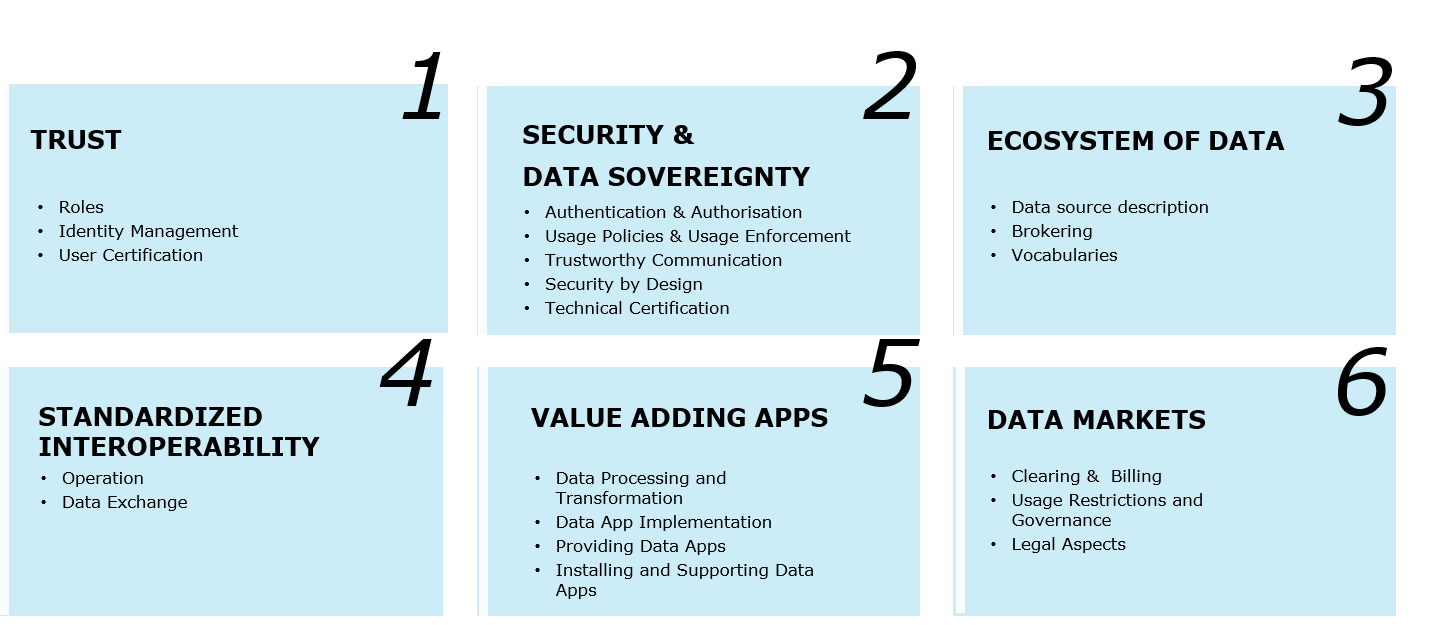
\includegraphics[width=6.44in,height=2.78in]{./media/image21.png}
		\caption{ Functional architecture of the International Data Spaces}
		\label{fig:_Functional_architecture_of_the_International_Data_Spaces}
	\end{Center}
\end{figure}


%%%%%%%%%%%%%%%%%%%% Figure/Image No: 13 Ends here %%%%%%%%%%%%%%%%%%%%


Figure \ref{fig:_Functional_architecture_of_the_International_Data_Spaces} shows the functional architecture of the International Data Spaces, subdividing the requirements into six groups of software functionality to be provided by the IDS. These six groups comply with the strategic requirements outlined in Section \ref{subsec:Goals_of_IDS}.



 The following subsections give a brief summary of these functional requirements. The full list of functional requirements can be found in a separate document entitled $``$Functional Overview$"$ .

\subsubsection{Trust}\label{subsec:functional_layer_trust}
%\addcontentsline{toc}{subsubsection}{Trust}

Although requirements related to trust are usually non-functional, they are addressed by the Functional Layer, since they represent fundamental features of the International Data Spaces. The $``$Trust$"$  group comprises three main aspects (roles, identity management, and user certification), which are complemented by governance aspects (see Section 4.3). %ToDo referer

\paragraph{Roles\\}
Each role in the International Data Spaces has certain rights and duties. For example, the Identity Provider is responsible for offering services to create, maintain, manage, monitor, and validate identity information of and for participants in the International Data Spaces. More information about the roles is given in Section 3.1. %ToDo: referer


\paragraph{Identity Management\\}
Every Connector participating in the International Data Spaces must have a unique identifier and a valid certificate. In addition, each Connector must be able to verify the identity of other Connectors (with special conditions being applied here; e.g., security profiles). 

\paragraph{User Certification\\}
Each participant in the International Data Spaces must undergo certification in order to establish trust among all participants. More information about the certification process is given in Section 4.2. %ToDo referer


\subsubsection{Security and Data Sovereignty}
%\addcontentsline{toc}{subsubsection}{Security and Data Sovereignty}
Like requirements related to trust, requirements related to security and data sovereignty are also usually non-functional, but are still addressed by the Functional Layer, since they represent fundamental features of the International Data Spaces. The $``$Security and data sovereignty$"$  group contains four major aspects: authentication $\&$  authorization; usage policies $\&$  usage enforcement; trustworthy communication $\&$  security by design; and technical certification.


\paragraph{Authentication $\&$  Authorization\\}
Each Connector must have a valid X.509 certificate. With the help of this certificate, each participant in the International Data Spaces that operates an endpoint is able to verify the identity of any other participant. Certain conditions (e.g. security profiles) may also apply here. More information about authentication is given in Section 4.1. % ToDo:referer

The Connector serving as the data source must be able to verify the receiving Connector’s capabilities and security features as well as its identity. More information about authorization is given in Section 4.1. %ToDo referer

\paragraph{Usage Policies $\&$  Usage Enforcement\\}
In the IDS, Data Owners and Data Providers can always be sure their data is handled by a Data Consumer according to the usage policies specified. Each participant can define usage policies and attach them to outbound data. Policies might include restrictions, such as disallowing persistence of data, or disallowing transfer of data to other parties, for example. More information about usage policies and usage enforcement is given in Section 4.1. % ToDo referer

\paragraph{Trustworthy Communication $\&$  Security by Design\\}
Connectors, App Stores, and Brokers can check if the Connector of the connecting party is running a trusted (i.e. certified) software stack. Any communication between (external) Connectors can be encrypted and integrity protected. Each Data Owner and Data Provider must be able to ensure that their data is handled by the Connector of the Data Consumer according to the usage policies specified: otherwise the data will not be sent. To reduce the impact of compromised applications, appropriate technical measures must be applied (e.g. isolating Data Apps from each other and from the Connector). Data Providers and Data Consumers can decide about the level of security to be applied for their respective Connectors by deploying Connectors supporting the selected security profile. More information about trustworthy communication and security by design is given in Section 4.1. %ToDo referer


\paragraph{Technical Certification\\}
The core components of the International Data Spaces, and especially the Connectors, require certification from the Certification Body in order to establish trust among all participants. More information about technical certification is given in Section 4.2. %ToDo referer


\subsubsection{Ecosystem of Data}
%\addcontentsline{toc}{subsubsection}{Ecosystem of Data}
Being able to describe, find and correctly interpret data is another key aspect of the International Data Spaces. Therefore, every data source in the International Data Spaces is described on the Information Layer (see section 3.4). % ToDo referer

The $``$Ecosystem of Data$"$  group comprises three major aspects: data source description, brokering, and vocabularies.


\paragraph{Data Source Description\\}
Participants must have the opportunity to describe, publish, maintain and manage different versions of metadata. Metadata should describe the syntax and serialization as well as the semantics of data sources. Furthermore, metadata should describe the application domain of the data source. The operator of a Connector must be able to define the price, the pricing model, and the usage policies regarding certain data. More information about data source description is given in Section 3.4. %ToDo referer


\paragraph{Brokering\\}
The operator of a Connector must be able to provide an interface for data and metadata access. Each Connector must be able to transmit metadata of its data sources to one or more brokers. Each participant must be able to browse and search metadata in the metadata repository, provided the participant has the right to access the metadata. Furthermore, each participant must be able to browse the list of participants registered at a broker. More information about brokering is given in Section 3.5.2. %ToDo referer


\paragraph{Vocabularies\\}
To create and structure metadata, the operator of a Connector may use vocabularies. In doing so, an operator of a Connector can use existing vocabularies, create own vocabularies, or work with other operators on new vocabularies provided by vocabulary hubs. Vocabulary hubs are central servers that store vocabularies and enable collaboration. Collaboration may comprise search, selection, matching, updating, requests for changes, version management, deletion, duplicate identification, and unused vocabularies. Vocabulary hubs need to be managed. More information about vocabularies is given in Section 3.4.%ToDo referer


\subsubsection{Standardized Interoperability}
%\addcontentsline{toc}{subsubsection}{Standardized Interoperability}
Standardized data exchange between participants is the fundamental aspect of the International Data Spaces. The IDS Connector is the main technical component for this purpose.

\paragraph{Operation\\}
Participants should be able to run the Connector software in their own IT environment. Alternatively, they can run a Connector on mobile or embedded devices. The operator of the Connector must be able to define the data workflow inside the Connector. Users of the Connector must be identifiable and manageable. Passwords and key storage must be protected. Every action, data access, data transmission, incident, etc. should be logged. Using this logging data, it should be possible to draw up statistical evaluations on data usage etc. Notifications about incidents should be sent automatically.


\paragraph{Data Exchange\\}
The Connector must receive data from an enterprise backend system, either through a push-mechanism or a pull-mechanism. The data can be provided via an interface or pushed directly to other participants. To do so, each Connector must be uniquely identifiable. Other Connectors can subscribe to data sources or pull data from these sources. Data can be written into the backend system of other participants.


\subsubsection{Value Adding Apps}
%\addcontentsline{toc}{subsubsection}{Value Adding Apps}
Before or after the actual data exchange, data may need to be processed or transformed. For this purpose, the International Data Spaces offers Data Apps. Each Data App has a lifecycle, spanning its implementation, provision in the App Store, installation, and support. The App Store should therefore be clearly visible and recognizable to every participant.

\paragraph{Data Processing and Transformation\\}
A data processing app (which is a subtype of a Data App) should provide a single, clearly defined processing function to be applied on input data for producing an expected output. A data transformation app (also a subtype of a Data App) should be able to transform data from an input format into a different output format in order to comply with the requirements of the Data Consumer (without any substantial change made to the information contained in the data; i.e., loss-less transformation). 

\paragraph{Data App Implementation\\}
The developers of Data Apps should be able to annotate the software with metadata (about functions and interfaces, pricing models, licenses, etc.). Data Apps must explicitly define their interfaces, dependencies, and access requirements.


\paragraph{Providing Data Apps\\}
Any authorized Data App developer can initiate a software provision process (App Store publication). Prior to publication in the App Store, Data Apps must pass an optional evaluation and certification process controlled by the Certification Body. The App Store should support authorized users in their search for a suitable application in an adequate fashion. Access of privileged users (e.g., administrators or operators) should require strong authentication (e.g., 2-factor authentication).


\paragraph{Installing and Supporting Data Apps\\}
A dedicated Connector service should support authorized users in (un-)installing Data Apps not originating from an official App Store. In addition, it should support authorized users in searching, installing, and managing (e.g., removal or automated updates) Data Apps retrieved from an App Store.


\subsubsection{Data Markets}
%\addcontentsline{toc}{subsubsection}{Data Markets}
Data to be exchanged in the International Data Spaces may have monetary value. Therefore, the International Data Spaces has to integrate data market concepts, like clearing and billing, but also governance.

\paragraph{Clearing $\&$  Billing\\}
The Data Owner can define the pricing model (e.g. pay per transfer, pay per access, pay per day/month/year), and the price of data. Any transaction of any participant can be logged. The clearing and billing process must be simple and standardized.


\paragraph{Usage restrictions, and governance\\}
Governance in the International Data Spaces comprises five aspects: data as an economic good, data ownership, data sovereignty, data quality, and data provenance. More information about governance is given in Section 4.3. %ToDO referer

\paragraph{Legal aspects\\}
Trading data on a data marketplace requires legal contracts and conditions that can be negotiated in an automated way. Therefore, standard contracts for typical data exchange transactions are necessary.  



 %%%%%%%%%%%%  include section 3.2 Process Layer here %%%%%%%%%%%%%%


\subsection{Process Layer}\label{subsec:process_layer}
%\addcontentsline{toc}{subsection}{Process Layer}
The Process Layer specifies the interactions taking place between the different components of the International Data Spaces. It thereby provides a dynamic view of the Reference Architecture Model. 

In the following, three major processes and their sub processes are described:



\begin{enumerate}
	\item \textbf{Onboarding,}  i.e. what to do to be granted access to the International Data Spaces as a Data Provider or Data User;

	\item \textbf{Exchanging data,} i.e. searching for a suitable Data Provider and invoking the actual data operation; and

	\item \textbf{Publishing and using Data Apps, }i.e. interacting with the IDS as an App Provider and user of a Data App, respectively.

\end{enumerate}\par



These three processes are related to the International Data Space's key value propositions and involve most of the roles introduced in the Business Layer section. The processes are illustrated using the Business Process Modeling Notation (BPMN).


\subsubsection{Onboarding}
%\addcontentsline{toc}{subsubsection}{Onboarding}
The overall $``$Onboarding$"$  process consists of several sub processes. The first step for an organization to join the International Data Spaces as a Data Provider or Data User is to acquire an identity to be used in the IDS. This identity, which forms the basis for establishing trusted communication in the IDS, is provided by the Certification Body and an Evaluation Facility in the form of a certificate issued by an Identity Provider. In a second step, the organization needs to request a Connector from a Software Provider. The Connector, being the core technical component for becoming part of the IDS, must then be installed. After that, it receives a digital certificate (X.509 certificate) to make sure it complies with IDS specifications and requirements. The digital certificate is based on the certification of the participant and the certification of the Connector (see section 3.1 and section 4.2).  In a third step, the Connector needs to be configured for internal use and prepared for secure communication ("Security Setup", see below). In the final step, the Connector needs to be made available for other participants in the IDS so that it can finally enter live operation. 
%ToDo referer

The overall $``$Onboarding$"$  process is illustrated in Figure \ref{fig:_Overall_onboarding_process}.The following paragraphs describe each step of the onboarding process in more detail.

%ToDo:update figure
%%%%%%%%%%%%%%%%%%%% Figure/Image No: 14 starts here %%%%%%%%%%%%%%%%%%%%

\begin{figure}[H]
	\begin{Center}
		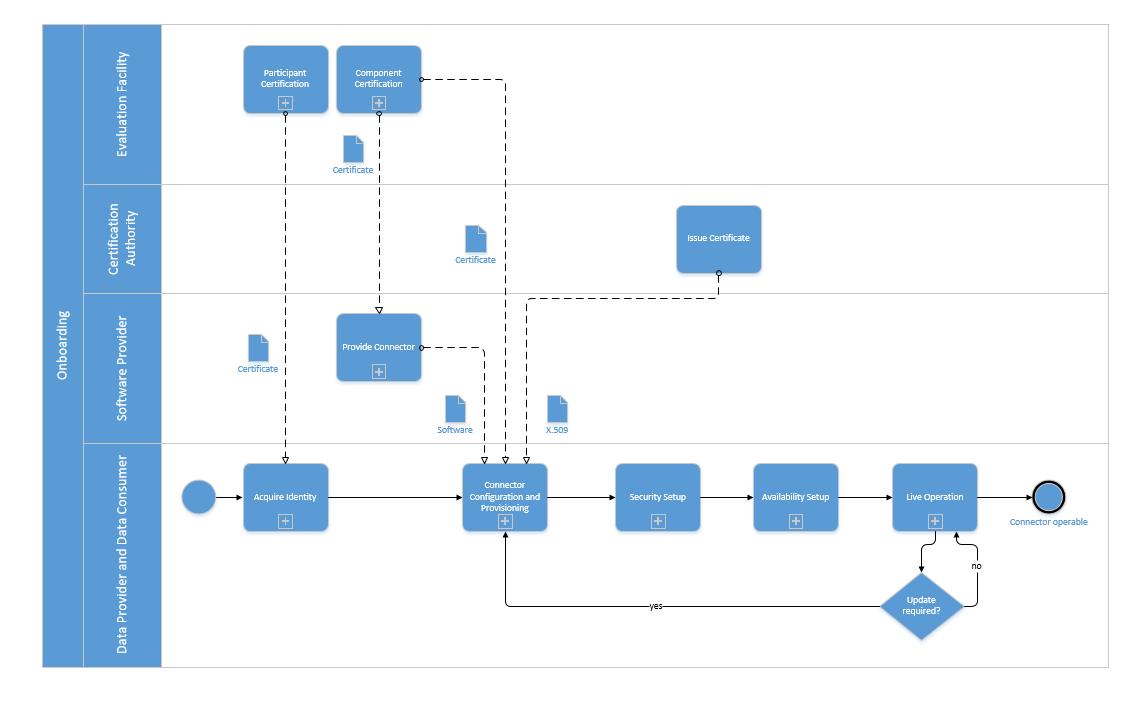
\includegraphics[width=6.53in,height=2.74in]{./media/image22.PNG}
		\caption{ $``$Onboarding$"$  overall process}
		\label{fig:_Overall_onboarding_process}
	\end{Center}
\end{figure}


%%%%%%%%%%%%%%%%%%%% Figure/Image No: 14 Ends here %%%%%%%%%%%%%%%%%%%%


\textbf{Acquire Identity}

Any organization that wants to operate a connector in order to exchange data in the International Data Spaces as a Data provider or Data Consumer needs to acquire a unique identity in the form of a certificate. This certificate enables them to establish secure and trusted connections to other IDS participants (see section 3.1).


\textbf{Connector Configuration and Provisioning}

Each Connector that participates in the IDS ecosystem must provide a self-description for other IDS participants to read, expressed in terms of the Information Model (see section 3.4). The respective organization needs to create this description at the beginning of the connector configuration and provisioning sub process. The Connector self-description must contain information about the respective organization, about who maintains the Connector (i.e. the Service Provider), and about the content and type of the data offered or requested.

Another mandatory step for the organization to take is to orchestrate data flows for (future) data retrieval and data provisioning, respectively, and to set up system adapters and communication interfaces ("endpoints"). (Details on the configuration of the IDS Connector are described in section 3.5.1.1.)

If needed, the organization can install and configure Data Apps acquired from the App Store.


%%%%%%%%%%%%%%%%%%%% Figure/Image No: 14 starts here %%%%%%%%%%%%%%%%%%%%

\begin{figure}[H]
	\begin{Center}
		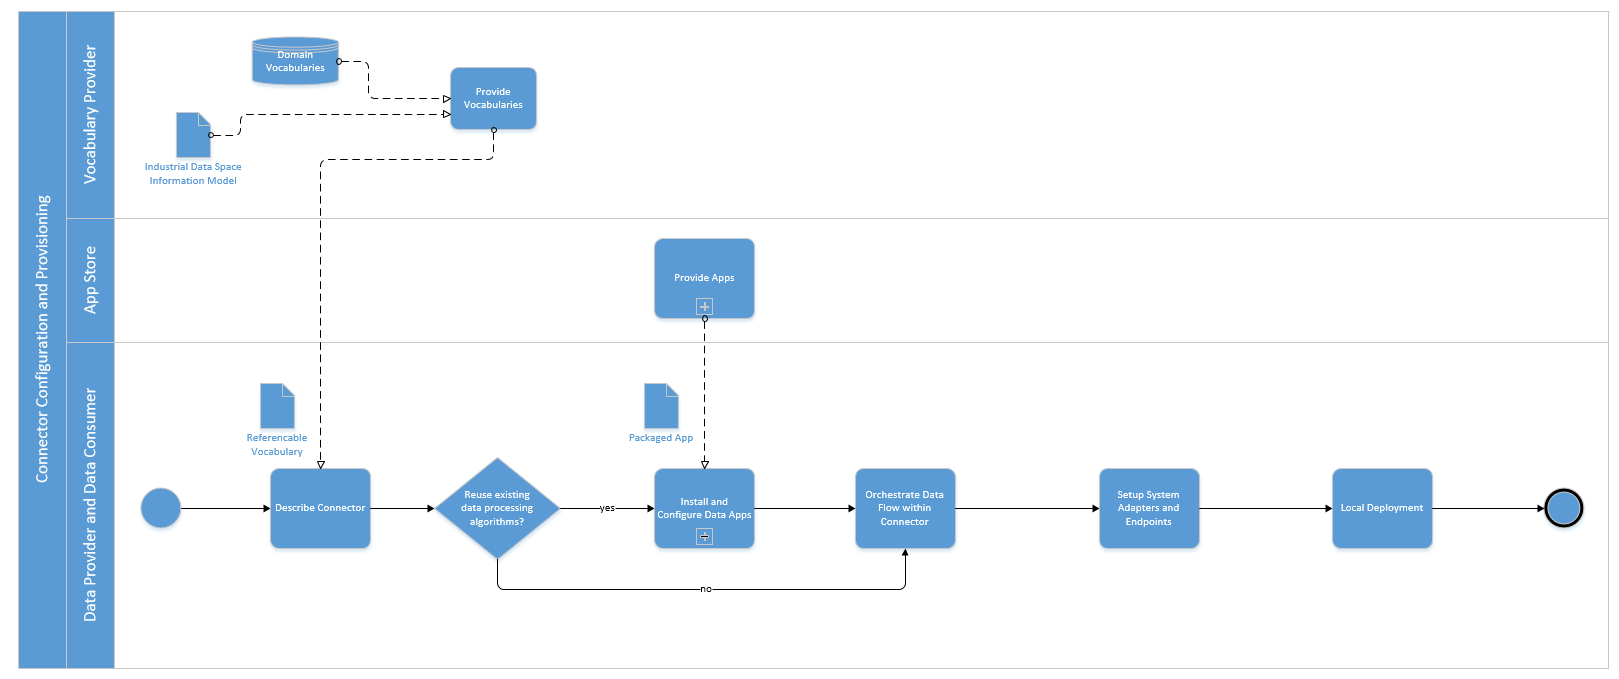
\includegraphics[width=6.53in,height=2.74in]{./media/image23.PNG}
		\caption{ $``$Connector Configuration and Provisioning$"$  sub process}
		\label{ fig:_Connector_Configuration_and_Provisioning_sub_process}
	\end{Center}
\end{figure}


%%%%%%%%%%%%%%%%%%%% Figure/Image No: 14 Ends here %%%%%%%%%%%%%%%%%%%%

\textbf{Security Setup}

To enable secure communication, a Certification Authority issues a certificate to the Data Provider or Data Consumer. This certificate is deployed locally to enable Transport Layer Security (TLS) and identification of the respective IDS participant. On top of that, the Connector self-description must be correct and valid, which is ensured by requesting a Dynamic Attribute Token from the Identity Provider (section 4.1) and validating the self-description against the Information Model. The token is a signed attestation that the information the Connector states about itself has been verified and is actually true. The token is presented by each subsequent outgoing communication message of the Connector, so that also the communicating Connectors have a means to verify the trustfulness of their communication partners at any time.

Furthermore, any organization that wants to assume the role of Data Provider or Data Consumer has the option to configure custom access restrictions for bilateral communications. For instance, a Data Provider may want to block certain Connectors or participants from accessing their services, or it may require specific access credentials. These configurations may be set up in the last step of the Security Setup sub process (see section 4.1).



%%%%%%%%%%%%%%%%%%%% Figure/Image No: 15 starts here %%%%%%%%%%%%%%%%%%%%

\begin{figure}[H]
	\begin{Center}
		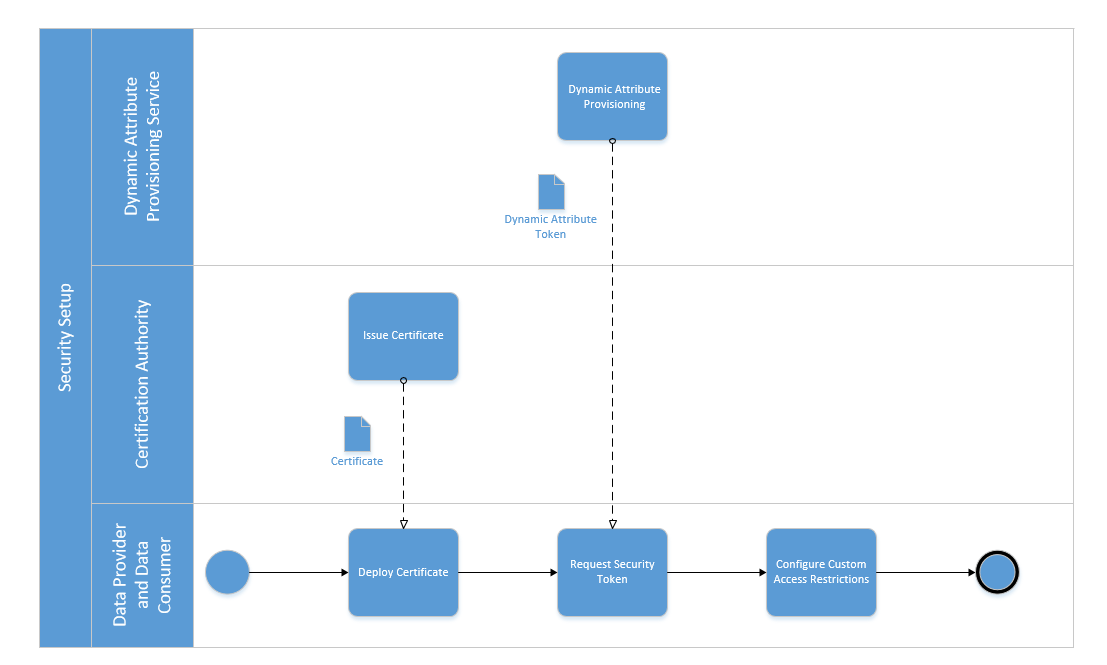
\includegraphics[width=7.03in,height=4.22in]{./media/image24.png}
		\caption{$``$Security Setup$"$  sub process}
		\label{fig:Security_Setup_sub_process}
	\end{Center}
\end{figure}


%%%%%%%%%%%%%%%%%%%% Figure/Image No: 15 Ends here %%%%%%%%%%%%%%%%%%%%

% check for Figure : \par


\textbf{Availability Setup}

After local Connector deployment and Security Setup, a Connector must be made available for other participants in the International Data Spaces. This is done by the provisioning of an $``$External Connector$"$ , which runs in a so-called $``$Demilitarized Zone (DMZ)$"$  and forwards or filters requests to the $``$Internal Connector$"$ . Alternatively, proper adjustment of firewall rules may be sufficient (in less sensitive environments). Each Data Provider and Data Consumer can decide whether or not they want to announce their Connector (or the data resources accessible through their Connector) publicly on the IDS. If they do so, they can select a Broker from a set of available Broker services (i.e., a registry for Connector self-descriptions) to publish the self-description of their Connector (see above). The Broker provides functions for searching for and retrieving registered Connector self-descriptions (see section 3.5.2), including data sources, interfaces, security profiles, and current levels of trustworthiness.



%%%%%%%%%%%%%%%%%%%% Figure/Image No: 16 starts here %%%%%%%%%%%%%%%%%%%%

\begin{figure}[H]
	\begin{Center}
		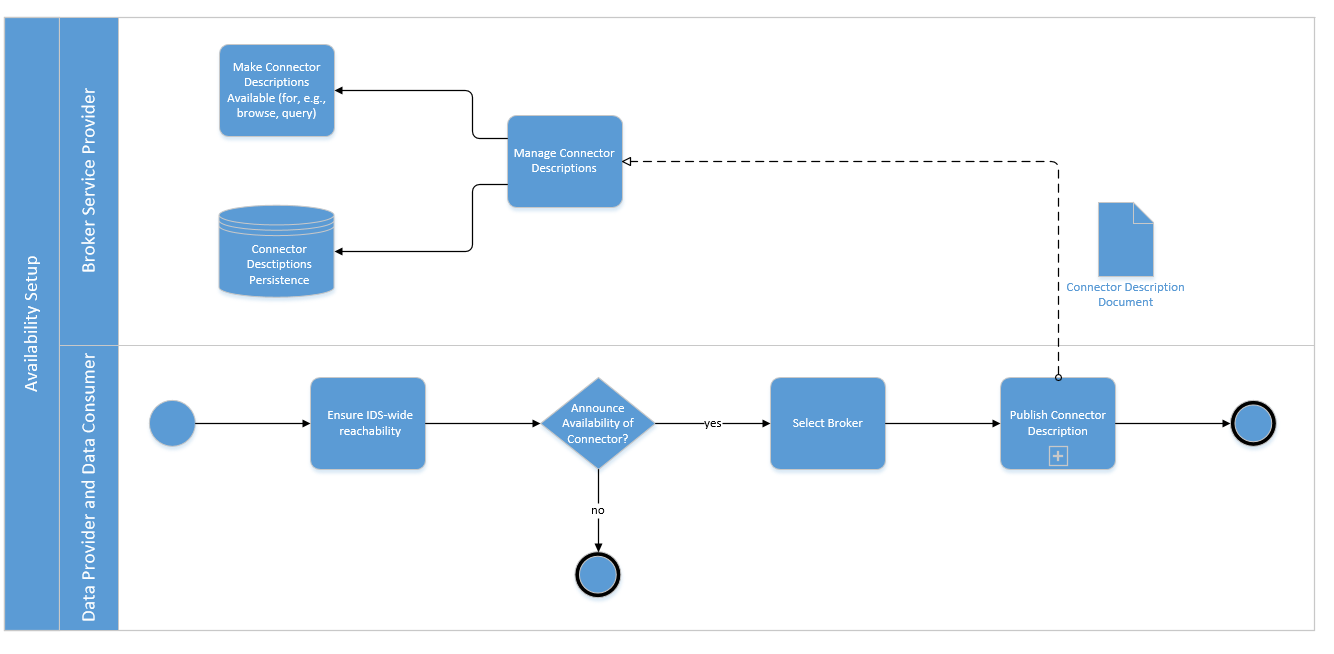
\includegraphics[width=6.25in,height=3.06in]{./media/image25.png}
		\caption{$``$Availability Setup$"$  sub process}
		\label{fig:Availability_Setup_sub_process}
	\end{Center}
\end{figure}


%%%%%%%%%%%%%%%%%%%% Figure/Image No: 16 Ends here %%%%%%%%%%%%%%%%%%%%



\subsubsection{Exchanging Data}
%\addcontentsline{toc}{subsubsection}{Exchanging Data}
The overall process of exchanging data consists of two sub processes, as illustrated in Figure \ref{fig:_Exchanging_Data__overall_process_}. The first sub process is about a Data Consumer searching for a suitable Data Provider. If the search was successful, the Data Consumer and the Data Provider can start to exchange data with one another. This is done after Connector configuration, either starting "from scratch" (see IDS onboarding process described above) or by reconfiguring an existing Connector. The second sub process is the invocation of the actual data operation (e.g. data upload or download, data transformation, or data query).

%%%%%%%%%%%%%%%%%%%% Figure/Image No: 17 starts here %%%%%%%%%%%%%%%%%%%%

\begin{figure}[H]
	\begin{Center}
		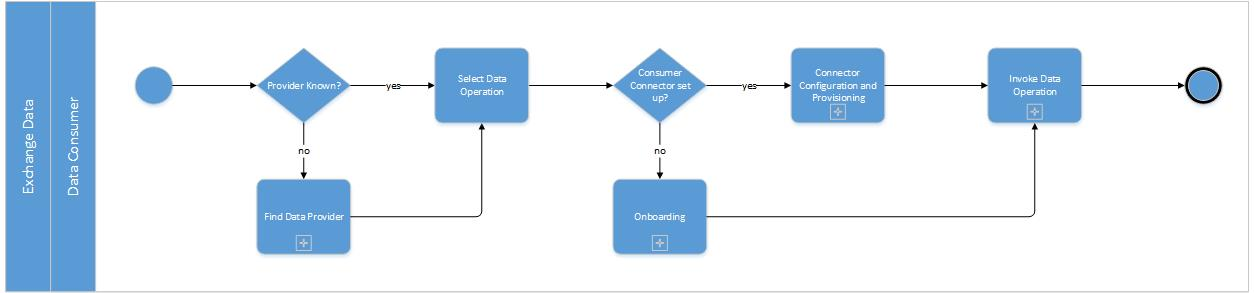
\includegraphics[width=6.53in,height=1.53in]{./media/image26.jpeg}
		\caption{ $``$Exchanging Data$"$  overall process }
		\label{fig:_Exchanging_Data__overall_process_}
	\end{Center}
\end{figure}


%%%%%%%%%%%%%%%%%%%% Figure/Image No: 17 Ends here %%%%%%%%%%%%%%%%%%%%


\textbf{Find Data Provider}

To find a Data Provider, the Data Consumer must send a query to a Broker Service Provider. Before that, however, the Data Consumer needs to select a suitable Broker (e.g. based on thematic coverage) and determine the query capabilities (e.g. a graphical search interface or a domain-specific query language). The Broker then returns the query result to the Data Consumer, who needs to interpret the result to find out about the different data sources available in the International Data Spaces for providing the data specified in the query. Each query result must provide information about each IDS Connector capable of providing the desired data, so that the Data Consumer can retrieve each Connector's self-description to learn more about how to receive the desired dataset from a technical point of view (e.g., endpoint addresses, protocol). The Data Provider may serve the same data using different representations or pricing options, so the Data Consumer may select a suitable offer from the Data Provider's Connector description.

Alternatively, the Data Consumer may already know a suitable Data Provider. In this case, the Data Consumer can contact the Data Provider directly (i.e. without invoking a broker).



%%%%%%%%%%%%%%%%%%%% Figure/Image No: 18 starts here %%%%%%%%%%%%%%%%%%%%

\begin{figure}[H]
	\begin{Center}
		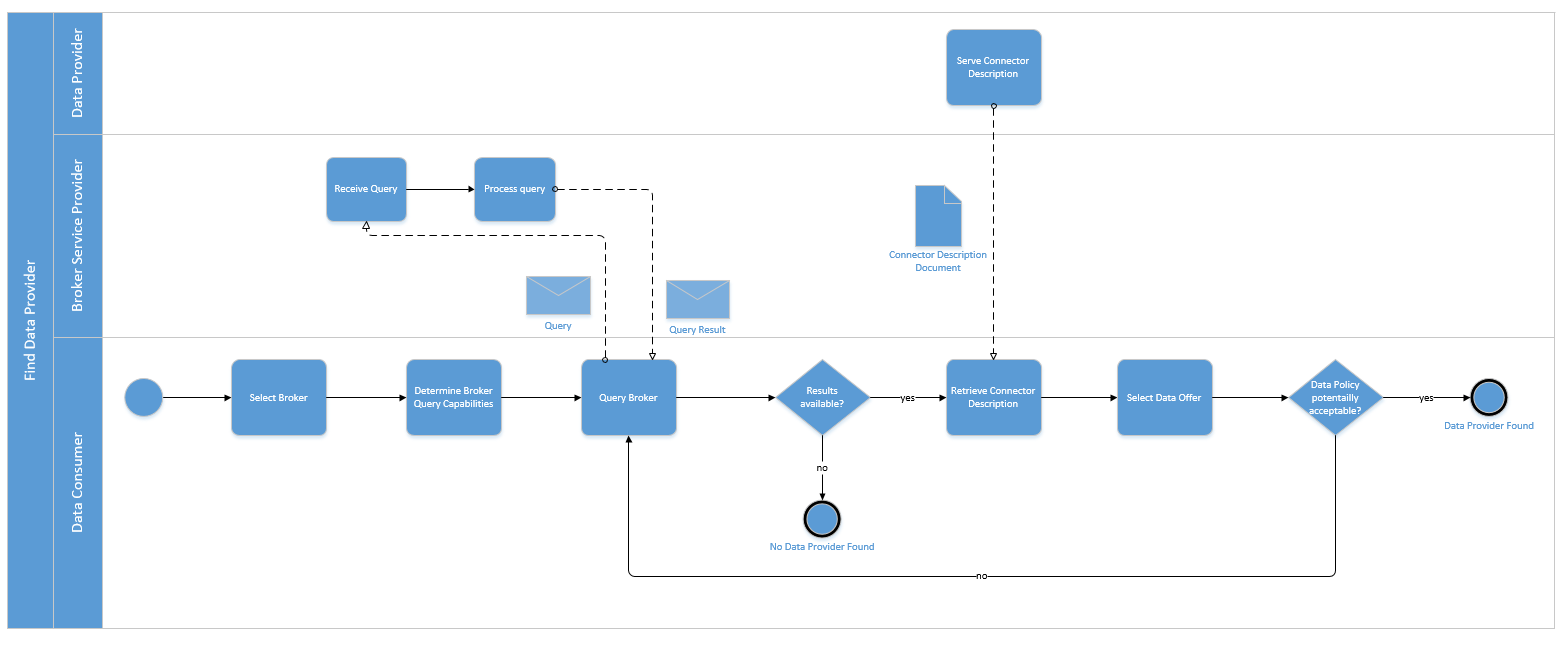
\includegraphics[width=6.53in,height=2.74in]{./media/image27.PNG}
		\caption{ $``$Find Data Provider$"$  sub process}
		\label{fig:_Find_Data_Provider__sub_process}
	\end{Center}
\end{figure}


%%%%%%%%%%%%%%%%%%%% Figure/Image No: 18 Ends here %%%%%%%%%%%%%%%%%%%%



\textbf{Invoke Data Operation}

Data usage policy information is an important element of legal agreements and is therefore modeled as first-class objects on the Information Layer (see Section 3.4). The handling of data usage policy information is shown in detail in the $``$Invoke Data Operation$"$  sub process (Figure \ref{fig:invole_data_operation}). While a Connector self-description basically contains information about the datasets available, also usage policy information can be extracted from this description. In a (semi-)automated negotiation process performed by the usage control frameworks of the participating Connectors, the Data Consumer and the Data Provider need to agree on a data usage policy. If an agreement has been reached, this policy is instantiated and deployed inside both Connectors. The policy both parties agree upon needs to be persisted in an immutable way by both sides. After the data usage policy has been established, the consuming Connector can be configured to deal with further data coming in from the Data Provider in the future as specified by the policy. The retrieval of the self-description and the negotiation of policies must make use of HTTPS or mqtt protocols. If this has been done, the Data Operation call can be invoked – this is usually done by a request using a common protocol (e.g., HTTP) to retrieve a data artifact from the Data Provider. 

The Data Provider then sends the result of the data operation to the Data Consumer. Usage control on both sides signals the data operation to the data provenance tracking infrastructure (accessible via the Clearing House), so that provenance information about the data transferred is kept up to date. Usage control on the Data Consumer side also signals receipt of the data operation result to the data provenance tracking infrastructure, in order to confirm that the transaction has been completed successfully (see sections 4.1.3.6 and 4.1.3.7). 


%%%%%%%%%%%%%%%%%%%% Figure/Image No: 19 starts here %%%%%%%%%%%%%%%%%%%%

\begin{figure}[H]
	\begin{Center}
		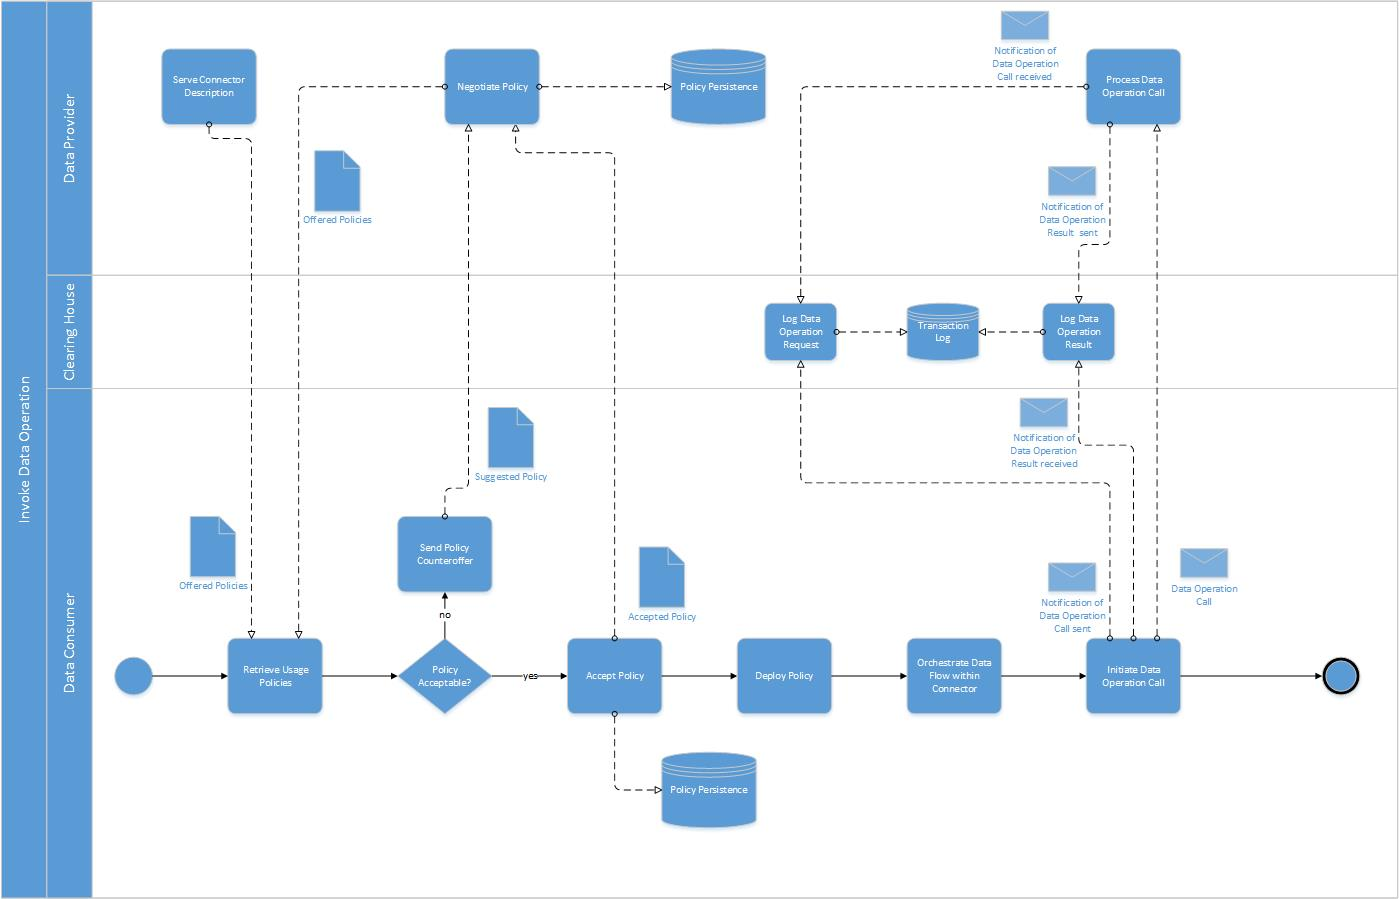
\includegraphics[width=6.53in,height=4.2in]{./media/image28.jpeg}
		\caption{$``$Invoke Data Operation$"$  sub process	}
		\label{fig:invole_data_operation}
	\end{Center}
\end{figure}


%%%%%%%%%%%%%%%%%%%% Figure/Image No: 19 Ends here %%%%%%%%%%%%%%%%%%%%

Communication between the Connectors can be asynchronous (i.e., the Data Consumer does not have to wait in idle mode for the result to arrive, but will be notified by the Data Provider as soon as the result is available). Instead of a pull-request, a push-request can be sent, which means that the Data Consumer asks for updates regarding the requested data. The updated data can be provided either after certain events (e.g., after the data has been updated by the Data Provider) or within certain time intervals (e.g., every five minutes). If a push-request is made, the Data Consumer repeatedly receives updated query results from the Data Provider. In case of a pull-request, the Data Consumer can repeat the last part of the process to query data again (using the same or a different query). The description of the communication pattern itself is not part of this document, as this is covered by existing standards (e.g. DIN SPEC 16593-1:2018-04, see chapter 8 $``$Characterizations of Interactions$"$ ) or as best practices in industry. 
		


\subsubsection{Publishing and Using Data Apps}
%\addcontentsline{toc}{subsubsection}{Publishing and Using Data Apps}
Data Apps can be used by Connectors for specific data processing or data transformation tasks. They can perform tasks of different complexity, ranging from simple data transformation to complex data analytics. An example of data transformation may be a Data App parsing a single string field with address information and producing a data structure consisting of street name and number, zip code, name of the city, and name of the country.\\
On a conceptual level, Data Apps can be treated the same way as data offerings in the International Data Spaces. Therefore, just as data is provided by a Data Provider using a Connector and registering this Connector at a Broker, Data Apps are created by an App Provider and registered at an App Store (using the App Provider's Connector as a means to communicate with the App Store). As a consequence, App Providers also need to undergo the Onboarding process. However, instead of registering their Connector at a Broker, App Providers register their Data Apps at an App Store.\\
In order to be published, certain Data Apps require certification from the Certification Body (see section 3.5.1) (see first step of the process shown in Figure \ref{fig:_Data_App_Certification__process}).



%%%%%%%%%%%%%%%%%%%% Figure/Image No: 20 starts here %%%%%%%%%%%%%%%%%%%%

\begin{figure}[H]
	\begin{Center}
		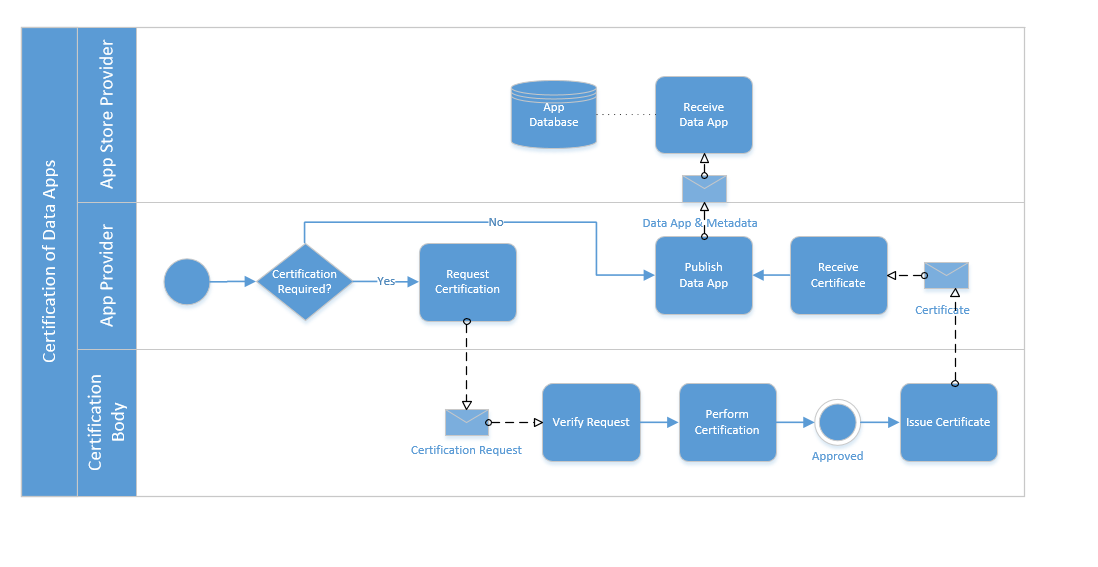
\includegraphics[width=6.47in,height=3.34in]{./media/image29.png}
		\caption{ $``$Data App Certification$"$  process}
		\label{fig:_Data_App_Certification__process}
	\end{Center}
\end{figure}


%%%%%%%%%%%%%%%%%%%% Figure/Image No: 20 Ends here %%%%%%%%%%%%%%%%%%%%



%%%%%%%%%%%%%%%%%%%% Figure/Image No: 21 starts here %%%%%%%%%%%%%%%%%%%%

\begin{figure}[H]
	\begin{Center}
		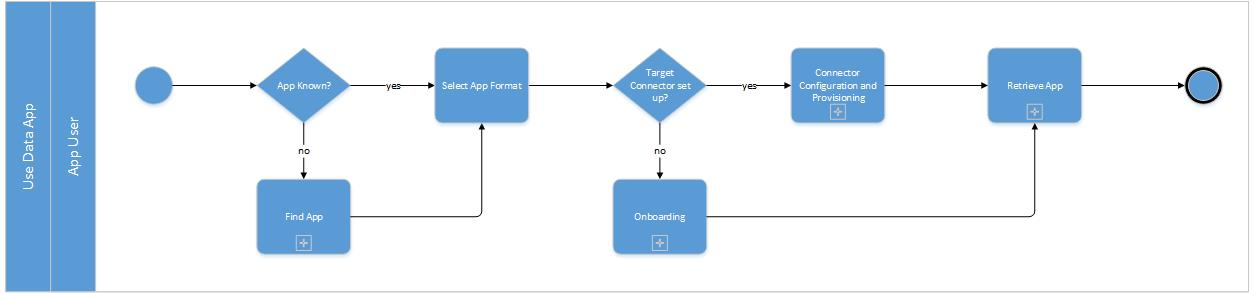
\includegraphics[width=6.53in,height=1.53in]{./media/image30.jpeg}
		\caption{Use Data App process}
		\label{fig:use_data_app}
	\end{Center}
\end{figure}
%%%%%%%%%%%%%%%%%%%% Figure/Image No: 21 Ends here %%%%%%%%%%%%%%%%%%%%

When it comes to using a Data App that is offered by an App Store, App Users (Data Provider or Data Consumer) need to execute a process that is very similar to the $``$Exchange Data$"$  process described above.
For each Data App that was successfully certified, the corresponding metadata is stored in the App Store for being retrieved by users (e.g., Data Consumers or Data Providers) via a search interface. Searching for a Data App is part of the “Find App” sub process depicted in Figure \ref{fig:use_data_app}. If a user finds a suitable Data App (i.e., matching in functionality and compatible with the user’s Connector packaging format) in the App Store, the App can be requested. This is indicated in the “Retrieve App” sub process, which is conceptually identical with the “Invoke Data Operation” process outlined in section 3.3.2, which is why a detailed discussion is omitted here.



 %%%%%%%%%%%%  include section 3.3 Process Layer here %%%%%%%%%%%%%%


\subsection{Information Layer}
%\addcontentsline{toc}{subsection}{Information Layer}
The Information Layer specifies the Information Model, the domain-agnostic, common language of the International Data Spaces. The Information Model is an essential agreement shared by the participants and components of the IDS, facilitating compatibility and interoperability. The primary purpose of this formal model is to enable (semi-)automated exchange of digital resources within a trusted ecosystem of distributed parties, while preserving data sovereignty of Data Owners. The Information Model therefore supports the description, publication and identification of data products and reusable data processing software (both referred to hereinafter as $``$Digital Resources$"$ , or simply $``$Resources$"$ ). Once the relevant Resources are identified, they can be exchanged and consumed via semantically annotated, easily discoverable services. Apart from those core commodities, the Information Model describes essential constituents of the International Data Spaces, its participants, its infrastructure components, and its processes.

The Information Model is evolved and maintained by the IDSA Sub-Working Group 4.\footnote{IDSA members may find further information at https://industrialdataspace.jiveon.com/community/workinggroups/architecture/swg4-information-model/.}

\subsubsection{Scope}
%\addcontentsline{toc}{subsubsection}{Scope}
The Information Model is a generic model, with no commitment to any particular domain. Domain modeling is delegated to shared vocabularies and data schemata, as provided e.g. by domain-specific communities of the International Data Spaces. The Information Model does not provide a meta-model for defining custom datatypes comparable to standards such as OData\footnote{https://www.odata.org/ } or OPC-UA\footnote{https://opcfoundation.org/ }. Concerns beyond the scope of modeling Digital Resources and their interchange are considered out of scope. The Information Model therefore does not deal with the side effects of data exchange (e.g. in scenarios in which data is used for time-critical machine operations).

\subsubsection{Model Representations}
%\addcontentsline{toc}{subsubsection}{Model Representations}
The Information Model has been specified at three levels of formalization. Each level corresponds to a digital representation, ranging from this high-level, conceptual document down to the level of operational code, as depicted in Figure \ref{fig:Representations_of_the_Information_Model}. Every representation depicts the complete Information Model in its particular way. Among the different representations, the Declarative Representation (IDS Vocabulary) is the only normative specification of the Information Model. As such, it is accompanied by a set of auxiliary resources (e.g. guidance documents, reference examples, validation tools, and editing tools intended to support a competent, appropriate, and consistent usage of the IDS Vocabulary).


\paragraph{Conceptual Representation \\}
%\addcontentsline{toc}{paragraph}{Conceptual Representation }
The Conceptual Representation of the Information Model presents a high-level overview of the main, largely invariant concepts, with no commitment to a particular technology or domain. It targets a general audience, management boards, and media, as it provides basic information and promotes a shared understanding of the concepts by means of a textual document and a plausible visual notation. If available, references to related elements of the Declarative Representation and a Programmatic Representation are provided, encouraging the reader to take a look at these alternative implementations.

\paragraph{Declarative Representation\\}
%\addcontentsline{toc}{paragraph}{Declarative Representation}
The Declarative Representation (IDS Vocabulary) provides a normative view of the Information Model of the International Data Spaces.\footnote{https://github.com/International-Data-Spaces-Association/InformationModel }
It has been developed along the analysis, findings, and requirements of the Conceptual Representation. Based on a stack of W3C Semantic Web technology standards\footnote{https://www.w3.org/standards/semanticweb/ } and standard modeling vocabularies (DCAT\footnote{https://www.w3.org/TR/vocab-dcat-2/ }, ODRL\footnote{https://www.w3.org/TR/odrl-model/ }, SKOS\footnote{https://www.w3.org/TR/skos-reference/ }, etc.), it provides a formal, machine-interpretable specification of concepts envisaged by the Conceptual Representation, residing at the persistent namespace URI \url{https://w3id.org/idsa/core/}. Furthermore, it details and formally defines entities of the International Data Spaces in order to be able to share, search for, and reason upon the structured metadata describing these entities. As such, it comprises a complete referential model allowing the derivation of a number of Programmatic Representations. The IDS Vocabulary is typically used and instantiated by knowledge engineers, ontology experts, or information architects. It defines a fairly minimal, domain-agnostic $``$core model$"$  and relies on third-party standard and custom vocabularies in order to express domain-specific facts. According to the common practice, existing domain vocabularies and standards are reused where possible, fostering acceptance and interoperability.


\paragraph{Programmatic Representation\\}
%\addcontentsline{toc}{paragraph}{Programmatic Representation}
The Programmatic Representation of the Information Model targets Software Providers by supporting seamless integration of the Information Model with a development infrastructure software developers are familiar with. It comprises a programming language data model (e.g., Java, Python, C++) shipped as a set of documented software libraries (e.g., JAR files).\footnote{https://github.com/International-Data-Spaces-Association/IDS-G/blob/master/repositories/README.md }
% ToDo: IDS-G should provide the single point of truth.  @Sebastian Steinbuß, this is the most specific link I can imagine.  However, that page does not have an easy-to-spot section "programmatic representation of the infomodel", but one has to search in order to find out that "Artifactory, Fraunhofer IAIS" provides the desired information, and this link could also still be improved (https://github.com/International-Data-Spaces-Association/IDS-G/issues/2).
The Programmatic Representation provides a best-effort mapping of the IDS Vocabulary onto native structures of a target programming language. This approach supports type-safe development, well-established unit testing, and quality assurance processes. It allows developers to easily create instances of the Information Model that are compliant with the IDS Vocabulary, relieving them from the intricacies of ontology processing.



%%%%%%%%%%%%%%%%%%%% Figure/Image No: 22 starts here %%%%%%%%%%%%%%%%%%%%

\begin{figure}[H]
	\begin{Center}
		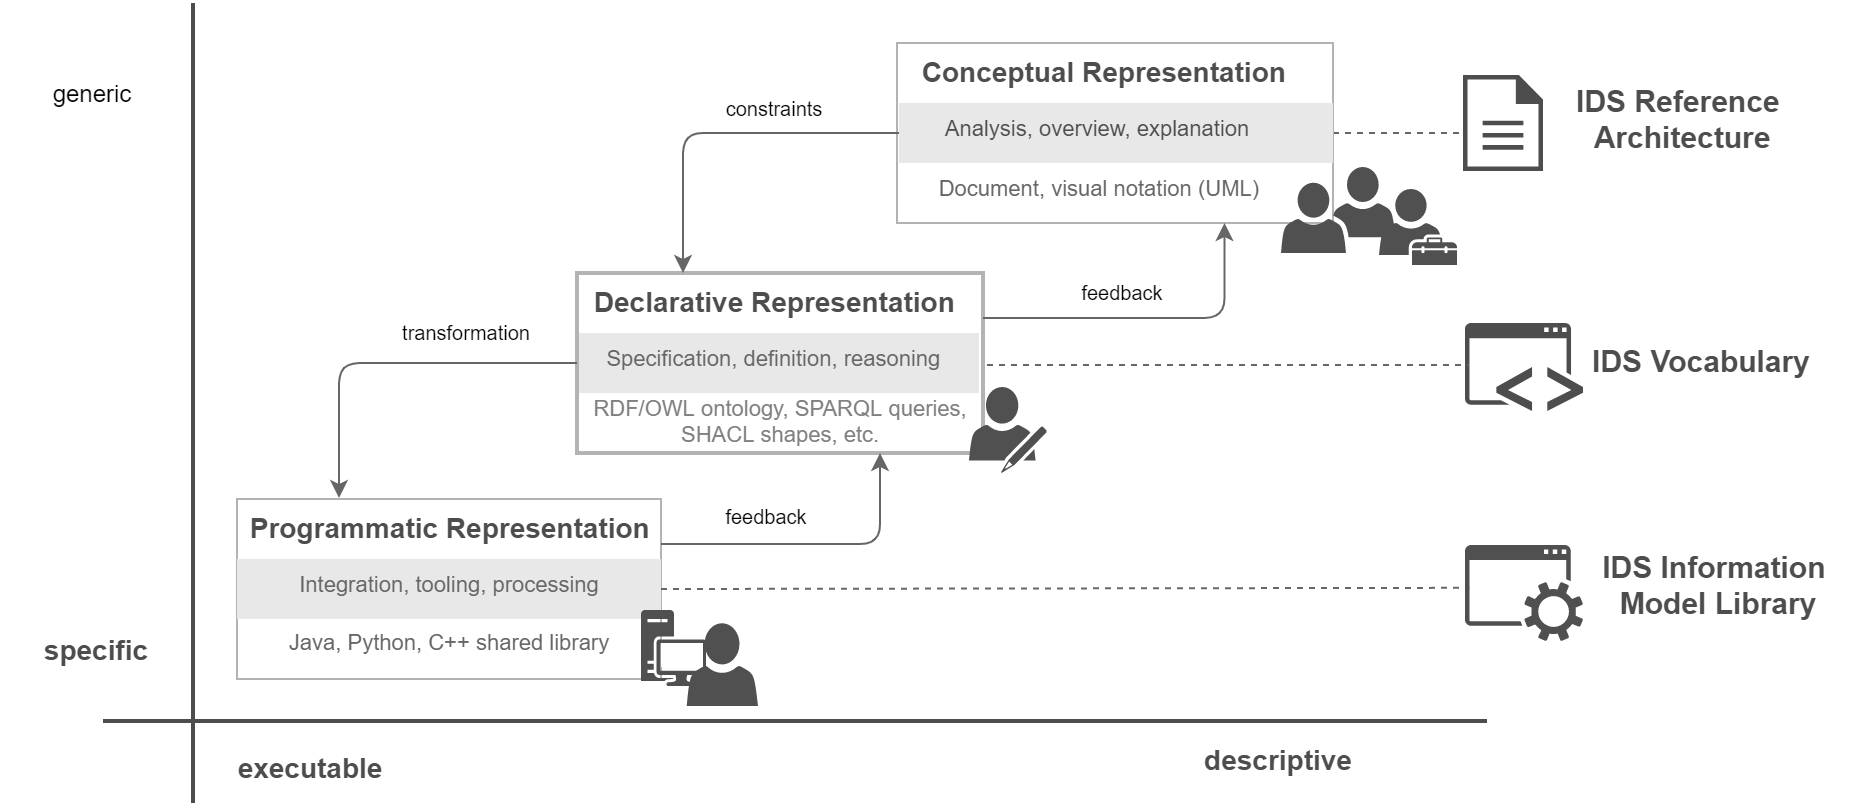
\includegraphics[width=6.53in,height=2.83in]{./media/image31.png}
		\caption{Representations of the Information Model}
		\label{fig:Representations_of_the_Information_Model}
	\end{Center}
\end{figure}


%%%%%%%%%%%%%%%%%%%% Figure/Image No: 22 Ends here %%%%%%%%%%%%%%%%%%%%


\subsubsection{Conceptual Representation of a Digital Resource in the IDS}
%\addcontentsline{toc}{subsubsection}{Conceptual Representation of a Digital Resource in the IDS}
In the following, the pivotal concept of a Digital Resource is introduced, segregated into modules in accordance with the $``$separation of concerns$"$  principle (SoC principle). To do so, a basic concern hexagon is gradually augmented by individual modeling aspects, resulting in a detailed version of the hexagon at the end of this section. To motivate acceptance and demonstrate the adequacy of the concern hexagon, a set of illustrative examples is introduced for each concern. The examples are motivated by a fictional scenario of observing traffic conditions at defined locations along the European highways for purposes of traffic control, predictive road maintenance, toll fee optimization, and so on.


\paragraph{Version Note\\}
%\addcontentsline{toc}{paragraph}{Version Note}
Since version 3.0 of the IDS-RAM, this section of the document has undergone minor changes, mainly providing more complete pointers to external standards reused by the Information Model.
Full versioning information is available from the repository hosting the source of the normative Declarative Representation.\footnote{In the repository referenced in section 3.4.2.2, see the top-level file \textit{CHANGELOG.md}.}
% ToDo: refer to sec 3.4.2.2


\paragraph{(Digital) Resource\\}
%\addcontentsline{toc}{paragraph}{(Digital) Resource}
A (Digital) Resource in the context of the International Data Spaces is a uniquely identifiable, valuable, digital (i.e. non-physical) commodity that can be traded and exchanged between remote participants using the IDS infrastructure. Following the web resource paradigm\footnote{ R. Fielding.  "Architectural Styles and the Design of Network-based Software Architectures," 2000.   PhD thesis.  Table 5-1 "REST Data Elements".  Available: https://www.ics.uci.edu/$ \sim $ fielding/pubs/dissertation/rest\_arch\_style.htm$\#$ tab\_5\_1 }, the abstract content of a Resource is provided in a variety of representations. Examples of Resources are documents, time series of sensor values, messages, image file archives, or media streams. Resources are subject to forwarding, processing, and/or consumption, with a particular demand for modeling related, complementary aspects (i.e., content, provenance, provisioning etc.). These are analyzed and specified here by applying the $``$separation of concerns$"$  (SoC) paradigm\footnote{ E. W. Dijkstra.  "On the role of scientific thought," EWD 447, 2000.  Available: http://www.cs.utexas.edu/users/EWD/ewd04xx/EWD447.PDF }.


\paragraph{Separation of Concerns (SoC)\\}
%\addcontentsline{toc}{paragraph}{Separation of Concerns (SoC)}
Following the $``$separation of concerns$"$  design principle, only one dimension of a subject matter is considered at a time, for the sake of clarity and consistency. Similar to the principle a microscope works, each concern follows a particular, analytical point of view, while other concerns can temporarily be disregarded. This principle can be applied to information modeling, aiming at a thorough understanding of the domain and fostering modularity and re-usability of the resulting (sub-) models. Accordingly designed, these models may evolve independently of each other and can be updated by different agents at different times. As any modification of a single element of the overall model does not require a change in other, logically unrelated parts, the development and maintenance of models can be substantially simplified. 


%%%%%%%%%%%%%%%%%%%% Figure/Image No: 23 starts here %%%%%%%%%%%%%%%%%%%%

\begin{figure}[h]
	\begin{Center}
		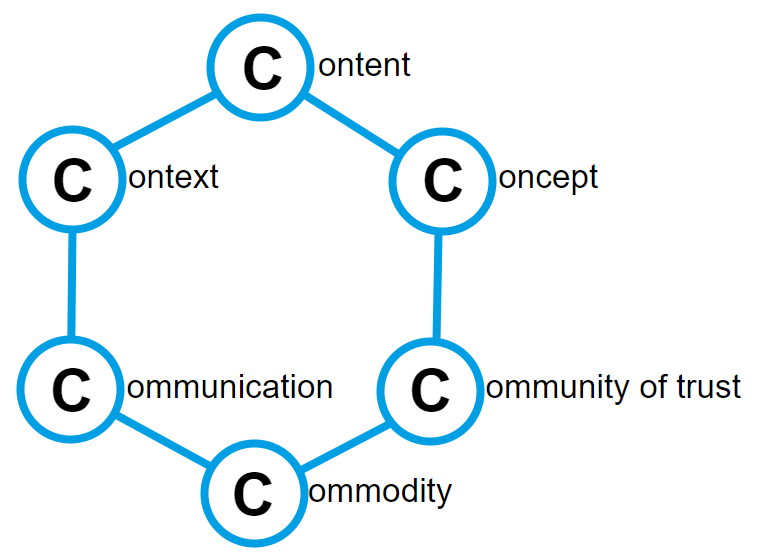
\includegraphics[width=3.64in,height=2.67in]{./media/image32.png}
		\caption{Outline of the Concern-Basic concern hexagon}
		\label{fig:Outline_of_the_ConcernBasic_concern_hexagon}
	\end{Center}
\end{figure}


%%%%%%%%%%%%%%%%%%%% Figure/Image No: 23 Ends here %%%%%%%%%%%%%%%%%%%%

\paragraph{Concern Hexagon\\}
%\addcontentsline{toc}{paragraph}{Concern Hexagon}
To illustrate the main modeling \uline{c}oncerns of Digital Resources in a way easy to memorize, the mnemonic hexagonal arrangement of \uline{c}arbon atoms can be used (C-Hexagon), as shown in Figure \ref{fig:Outline_of_the_ConcernBasic_concern_hexagon}. As a Resource’s content is its most essential aspect, Content is located at the top of the hexagon. This content is interpretable by references to a shared, formally defined Concept, whereas links to a particular \textit{C}ontext\textit{ }(in terms of time, place, or real-world entities) make the content potentially relevant for certain Data Consumers. So the upper part of the C-Hexagon deals with the "what" aspects, independently of Data Exchange, Data Sharing or Data Utilization. The lower part relates to the "how" aspects; i.e. how the content is exchanged (\textit{C}ommunication) and under which conditions (\textit{C}ommodity). The \textit{C}ommunity of Trust concern refers to the distinctive feature of the International Data Spaces being an ecosystem of certified participants and components that exchange and share Digital Resources in accordance with usage policies ensuring data sovereignty.

The level of detail differs across the individual concerns. The selection of their constituting aspects may change in light of new requirements and insights. Modeling concerns may inform, but do not necessarily correspond to any physical organization of the model (e.g., modules or directories). Some of the models listed below directly map to the above mentioned concerns, while others take a more detailed perspective on particular aspects.

\paragraph{Content\\}
%\addcontentsline{toc}{paragraph}{Content}


The \textit{Content }concern deals with the description of a Resource’s inherent substance, i.e. its $``$content$"$  available in any machine-interpretable, binary format. It addresses questions like: 
 \begin{itemize}
	\item What type of content does a Resource provide (e.g. text or an image)? 
 	\item What does the content look like (i.e. what is its structure, format etc.)? 
 	\item Is a content sample provided? 
 	\item What is the size and creation date of a particular file?
\end{itemize} 

At the abstract \textit{Resource} level, content is described independently of its physical manifestation. It is made concrete by augmenting structural information, i.e. details of how content is serialized into one of the supported \textit{Representations. }At a certain point in time, a Representation materializes in one or several \textit{Instances} (e.g. values or files).
These different levels of abstraction follow the principles of the Data Catalog Vocabulary (DCAT)\footnote{https://www.w3.org/TR/vocab-dcat-2/}.\\

\begin{figure}[H]
	\begin{Center}
		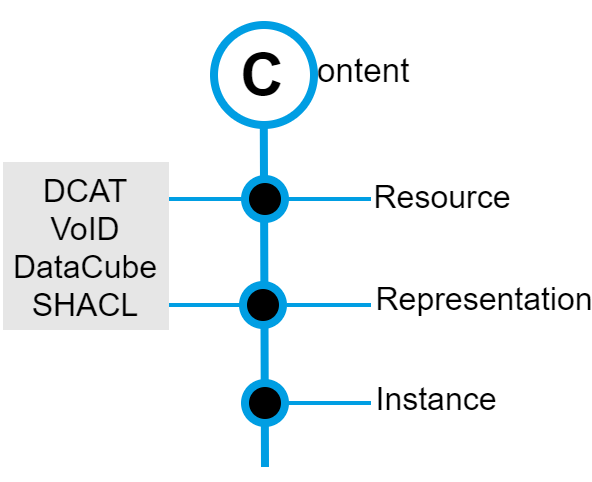
\includegraphics[width=2.0in,height=2.61in]{./media/image33.png}
		\caption{Outline Content Concern}
		\label{fig:outline_content_concern}
	\end{Center}
\end{figure}


\subparagraph*{Resource }
%\addcontentsline{toc}{subparagraph}{Resource}
Digital content at the Resource level of description abstracts away from a particular physical manifestation and deals with aspects that are shared equally by any of the content’s embodiments. 

Example: A \textit{report (i.e. Text, see below) containing figures regarding the utilization of European highways since 2000}.



\textbf{RESOURCE TYPE} There are various types of Digital Resources\footnote{ https://tools.ietf.org/html/rfc2046 },\footnote{\ \  http://dublincore.org/documents/dcmi-terms/$\#$ section-7 }. Resources may differ with regard to the intended purpose, the level of structuring, or the (sensory) requirements for its consumption and interpretation. Distinguished sets of properties are expected to evolve per Resource type, depending on their (future) use and relevance. 

Regarding the IDS-RAM, \textit{Data }is defined in alignment with ISO/IEC 2382:2015\footnote{ https://www.iso.org/standard/63598.html } (Information technology – Vocabulary)  as a statement of facts provided in a formalized, structured format intended primarily for machine processing (i.e. atomic values or arrangements of data fields, optionally defined by a schema). \textit{Text }represents a meaningful sequence of characters written in human language, which is intended for being read and interpreted by humans (or other intelligent agents) regardless of its Representation (e.g. document or screenshot image). \textit{Audio }refers to media content primarily intended for aural perception; consumption of such content normally requires an audio output device (i.e. a loudspeaker). \textit{Image }is static (i.e. time invariant) media content intended for visual perception, normally requiring a display device (i.e. a screen). \textit{Video }is dynamic (i.e. time variant) media content intended for visual and aural perception, combining the rendering requirements of Image and Audio as well as further requirements on processing (decoding etc.). \textit{Software} is a collection of machine-interpretable instructions, such as executable software (binary), program code (source), or fragments thereof; after optional preprocessing (compilation, installation etc.) its intended purpose is a subsequent execution exposing functionality. \textit{Opaque} is another, unspecified type of custom, binary content. The \textit{Container} is a collection of multiple (implicit) content elements that are distributed as a single unit (archive). 



%%%%%%%%%%%%%%%%%%%% Figure/Image No: 24 starts here %%%%%%%%%%%%%%%%%%%%

\begin{figure}[H]
	\begin{Center}
		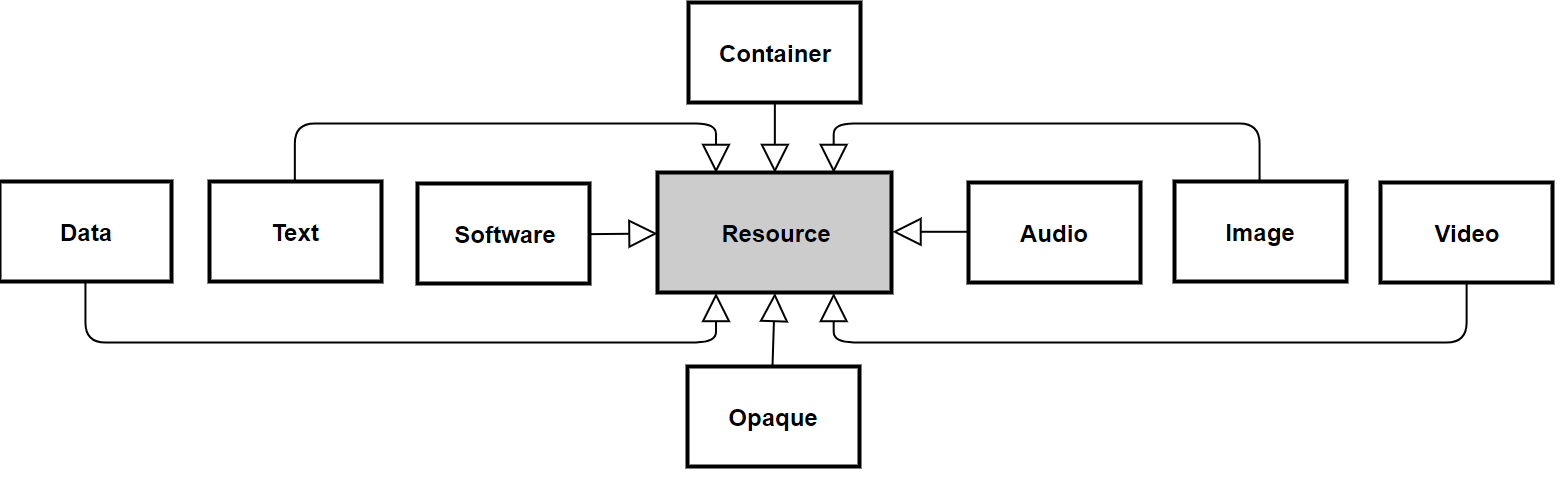
\includegraphics[width=6.53in,height=2.02in]{./media/image34.png}
		\caption{Taxonomy of the Resource concept}
		\label{fig:Taxonomy_of_the_Resource_concept}
	\end{Center}
\end{figure}


%%%%%%%%%%%%%%%%%%%% Figure/Image No: 24 Ends here %%%%%%%%%%%%%%%%%%%%



\textbf{HIERARCHY} Individual, physically or logically $``$included$"$  parts of the Container (e.g. an archive file), as well as any other structured Resource (e.g. software re-using 3\textsuperscript{rd} party libraries), may explicitly be referred to by the \textit{content-part} relation\footnote{http://dublincore.org/documents/dcmi-terms/$\#$ terms-hasPart }, allowing the modeling of part-whole hierarchies.

\textbf{CONTEXT} Temporal, spatial and real-world entities linked to the Resource content are covered by the Context concern (see section 3.4.3.6).

\textbf{CONCEPT} Semantic annotation of the Resource content is covered by the Concept concern for the Resource as a whole (see section 3.4.3.7),
% ToDo: referer (link was wrong in RAM 3.0)
and by links to domain-specific vocabularies for a more detailed view (realized using VoID, Data Cube and SHACL, as explained in section 3.4.4).
% ToDo: referer



%%%%%%%%%%%%%%%%%%%% Figure/Image No: 25 starts here %%%%%%%%%%%%%%%%%%%%

\begin{figure}[H]
	\begin{Center}
		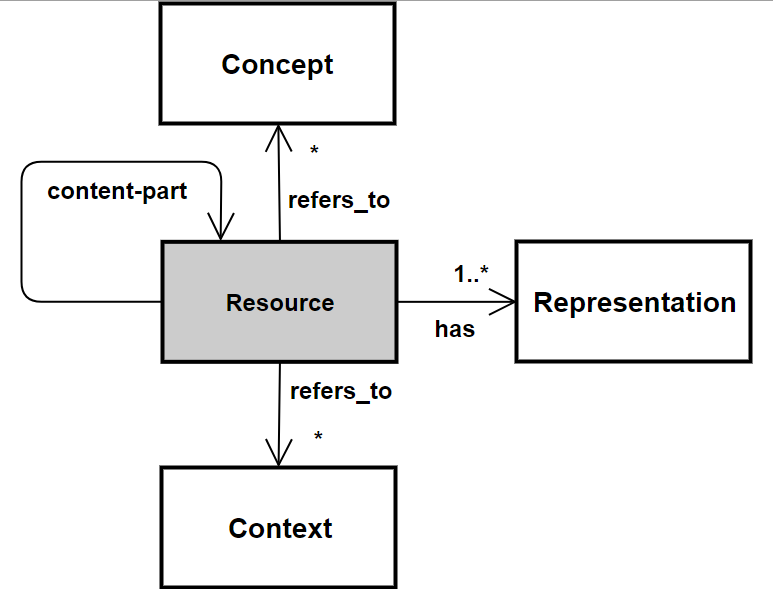
\includegraphics[width=3.44in,height=2.74in]{./media/image35.png}
		\caption{Resource concept (outline)}
		\label{fig:Resource_concept_outline}
	\end{Center}
\end{figure}


%%%%%%%%%%%%%%%%%%%% Figure/Image No: 25 Ends here %%%%%%%%%%%%%%%%%%%%


\subparagraph*{Representation}
%\addcontentsline{toc}{subparagraph}{Representation}
Abstract Resource content can be made $``$concrete$"$  by adding serialization details, i.e. by specifying alternative, physical Representations of the content. For example, Image content might be exposed via raster (JPEG, PNG, GIF) or vector graphics Representations (SVG). Developers of a „software for image anonymization$"$  might provide alternative software Representations (Windows EXE, Debian DEB, or Java JAR) supporting different software environments and operating systems. 

Example: \textit{The above mentioned report made available in a PDF or MS Word format}. 

\textbf{TYPE} The general physical arrangement of the content is indicated by the Internet Media Type (MIME-Type) and, if appropriate, more specifically by its specific data type.

\textbf{SCHEMA} Schema documents provide a formal structure definition of a Data Resource type. Profiles may add additional, selective constraints that apply to a subset of the considered data (e.g. geospatial data)\footnote{As an example, consider DCAT-AP, the DCAT Application Profile for data portals in Europe: https://joinup.ec.europa.eu/solution/dcat-application-profile-data-portals-europe }.

\textbf{PACKAGING} Packaging refers to means for archiving, compressing, and encrypting a Representation in a transparent, generic way.



%%%%%%%%%%%%%%%%%%%% Figure/Image No: 26 starts here %%%%%%%%%%%%%%%%%%%%

\begin{figure}[H]
	\begin{Center}
		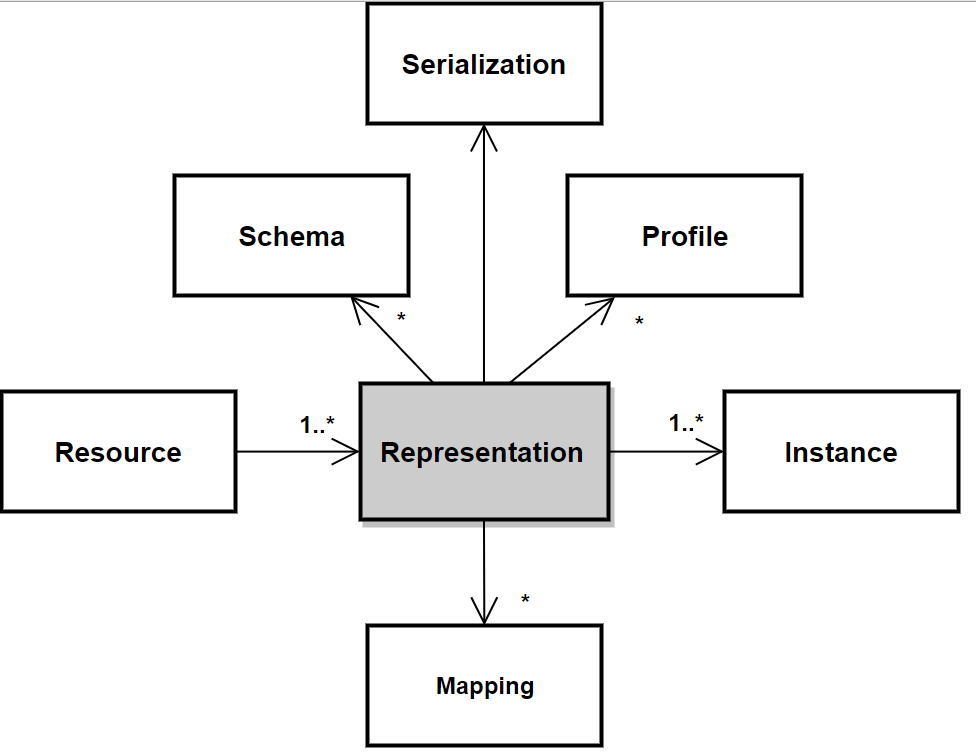
\includegraphics[width=4.03in,height=3.12in]{./media/image36.png}
		\caption{Representation concept (outline)}
		\label{fig:Representation_concept_outline}
	\end{Center}
\end{figure}


%%%%%%%%%%%%%%%%%%%% Figure/Image No: 26 Ends here %%%%%%%%%%%%%%%%%%%%


\subparagraph*{Instance}
%\addcontentsline{toc}{subparagraph}{Instance}
At a certain point in time, a Representation materializes into instances, which are either transient values or persisted files (Artifacts). Going beyond the prototypical level of Representation, an Instance captures properties that are unique to this materialization of the Resource’s content or particular elements thereof. 



Example: \textit{Version 3.1 of the above mentioned report; date of creation: 2018/01/17; file size: 1,73 MB (PDF) and 1,81 MB (MS Word), respectively}.



\textbf{IDENTITY} A rendered artifact may be provided with (partial) identity features, such as a file name or hash sum. It becomes identifiable and distinguishable from other artifacts, and is suited for file-oriented provision. (Representations, in contrast, are suited for interactive, service-oriented provision, due their nature of being prototypical „blueprints$``$.) 

\textbf{SIZE }The Size (specified e.g. in bytes) is another inherent characteristic of an artifact. 



\paragraph{Context\\}
%\addcontentsline{toc}{paragraph}{Context}
The \textit{Context} concern deals with temporal and spatial aspects as well as with real-world entities a Resource’s content relates to (intrinsic context). It addresses questions like: 
 \begin{itemize}
	\item What time period does the content cover? 
 	\item When and where was it gathered? 
 	\item Which sub-entity of a larger entity does a certain dataset relate to?
\end{itemize} 
Accurate context modeling helps a client in searching for and assessing the relevance of a Resource with respect to her informational needs, for example, by looking at most recent data (\textit{Time}) available for water pipelines (\textit{Entity}) within a particular area of interest (\textit{Space}) 


\begin{figure}[H]
	\begin{Center}
		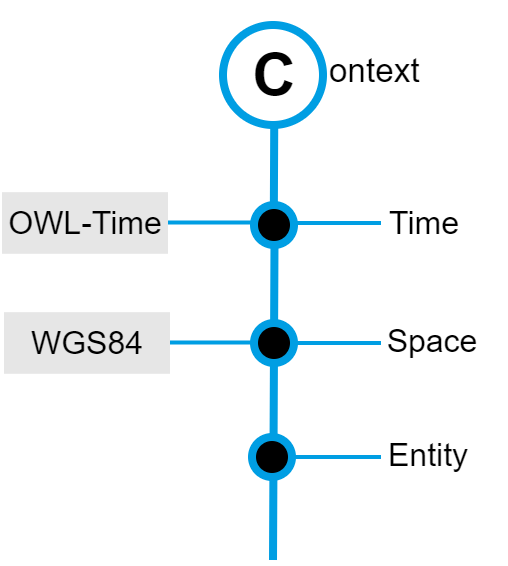
\includegraphics[width=1.33in,height=2.68in]{./media/image37.png}
		\caption{Outline Context Concern}
		\label{fig:outline_context_concern}
	\end{Center}
\end{figure} 


\subparagraph*{Time and space}
%\addcontentsline{toc}{subparagraph}{Time and space}
Time and space are quantifiable context dimensions usually expressed by coordinates with regard to a shared reference system, such as Coordinated Universal Time (UTC\footnote{https://www.itu.int/dms\_pubrec/itu-r/rec/tf/R-REC-TF.460-6-200202-I!!PDF-E.pdf }) or World Geodetic System 1984 (WGS 84\footnote{http://earth-info.nga.mil/GandG/publications/tr8350.2/wgs84fin.pdf }), allowing for unambiguous interpretation. One-dimensional temporal context is limited to either a single point in time (instant) or an interval with a non-empty duration. Thanks to the linear nature of time, open-end intervals may express a continuous period with only an endpoint defined\footnote{Cf. the Library of Congress Extended Date/Time Format (EDTF, https://www.loc.gov/standards/datetime/edtf.html) and the W3C OWL-Time ontology (https://www.w3.org/TR/owl-time/). }. In contrast to temporal context, spatial context is capable of expressing two-dimensional and three-dimensional shapes as bounding boxes defined by a set of coordinates. 

Example: \textit{Time period covered by the report, starting on January 1, 2000 UTC (end time is undefined here, as the report is continuously updated)}. 


\subparagraph*{Real-world entities}
%\addcontentsline{toc}{subparagraph}{Real-world entities}
This type of \textit{qualitative} context refers to identifiable temporal and spatial entities, i.e. which are (implicitly) defined by spatio-temporal coordinates. These are conventionalized \textit{named entities}, such as time periods\footnote{https://en.wikipedia.org/wiki/List\_of\_time\_periods } ($``$Renaissance$"$ ), country codes (according to ISO 3166\footnote{https://www.iso.org/iso-3166-country-codes.html }), national\footnote{https://de.wikipedia.org/wiki/Liste\_der\_Bundesautobahnen\_in\_Deutschland } and international road names (ECE/TRANS/SC.1/2016/3/Rev.1\footnote{https://www.unece.org/trans/main/sc1/sc1doc\_2016.html }) etc. Being based upon an established reference system, standard, or convention, such entities are considered universally valid. In addition, within restricted domains (e.g. a building), \textit{custom context entities} may be defined (e.g. individually numbered rooms), serving the purposes of contextualizing data (e.g. for sensor observations). The usability of custom context entities is limited by the characteristics of the defining model, i.e. being a machine-interpretable, widely accepted one \textbf{(}ISO 16739\footnote{https://www.iso.org/standard/70303.html }), and the context entities themselves. These should have a (semantic) type or \textit{concept} information attached in order to support general, categorical queries for data (e.g. temperature sensed in all $``$laboratories$"$ ). This type of annotation is, among others, supplied by the \textit{Concept }concern. 

Example: \textit{$``$A 555$"$ , Germany’s first highway ever built, connecting the cities of Bonn and Cologne, which is mentioned in the report}. 

\paragraph{Concept\\}
%\addcontentsline{toc}{paragraph}{Concept}
 The \textit{Concept }concern deals with the modeling of the $``$meaning$"$ , annotation, and interpretation of entities introduced by the orthogonal Resource concerns (Content, Context, Communication etc.). It addresses questions like:  \begin{itemize}
	\item What type of observation does the data refer to $``$temperature$"$  ? 
 	\item What kind of object does a context entity represent (factory, building)? 
 	\item What is the meaning of a certain date parameter (beginning or end of a range)?
\end{itemize} 
 \textit{Keywords }express the $``$meaning$"$  of an entity via informal natural language tags. As keywords can be chosen freely by a Data Provider, they are prone to inconsistencies and errors. Using controlled vocabularies, it is possible to add curated, (formally) defined and reusable \textit{Terms}, which can be shared across different scenarios and domains. In addition, conceptual schemas and ontologies define \textit{Types} of entities, if these are to be individually modeled as custom instances.  

\begin{figure}[H] 			
	\begin{Center}
		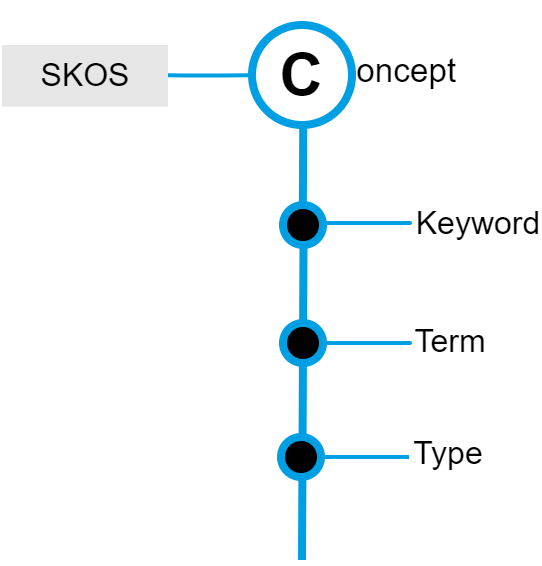
\includegraphics[width=1.46in,height=2.77in]{./media/image38.png}
		\caption{Outline Concept Concern}
		\label{fig:outline_concept_concern}
	\end{Center}
\end{figure}

\textbf{KEYWORD} Keywords are natural language annotations (tags) arbitrarily chosen by the Data Provider to accurately characterize the Resource from their perspective. As such, they are likely to be subjective and more domain specific than general terms provided by controlled vocabularies. Consistency and alignment of custom tag sets can be supported by means of documentation (guidance), editing tools (tag suggestions), or quality gates during the publication process, for example. 

Examples: \textit{$``$statistics$"$ , $``$highway$"$ , $``$usage$"$ , $``$traffic$"$ , $``$Europe$"$ .}

\textbf{TERM} In contrast to (arbitrarily chosen) keywords, terms are normally retrieved from an authoritative, curated source of definition (controlled vocabulary) or defined as instances of a conceptual type system, implemented, e.g., using the SKOS Simple Knowledge Organization System\footnote{https://www.w3.org/TR/skos-reference/}. Identified by a normative literal (code) or a unique identifier (URI), each term represents a reusable concept ($``$singleton$"$ ) that can be shared across different usage scenarios and domains without variations. 

Example: \textit{http://example.org/traffic\_statistics}. 

\textbf{TYPE} Terms are not capable of expressing individual characteristics of annotated entities. For this purpose, conceptual schemas and ontologies define \textit{types} of entities (e.g. classes, concepts) along with properties and relations their instances may adopt. Unlike terms, instances of a type convey the custom, particular semantics of the modeled entity. Conceptual types may be extended (specialized) to meet the requirements of other domains. 

Example: \textit{http://example.org/TabularTrafficReport.}\par

\paragraph{Communication\\}
%\addcontentsline{toc}{paragraph}{Communication}


The \textit{Communication }concern deals with means to communicate a Resource’s content in one of the Representations available. It addresses questions like:  \begin{itemize}
	\item Is there any input required on client to retrieve the content?  	
	\item What communication protocols are supported? 
 	\item What does a valid request look like? 
 	\item What is the address of the endpoint handling the request?
\end{itemize} 
 \textit{Operations} are the building blocks of interactive interfaces for sharing and processing a Resource’s content. They model an abstract functionality along with involved parameters and underlying interaction patterns. Through bindings to a communication protocol, operations become $``$concrete$"$  and can be invoked at networked \textit{Endpoints}. A Connector’s interactions at these Endpoints can be complemented by \textit{Message} metadata.


\begin{figure}[H]
	\begin{Center}
		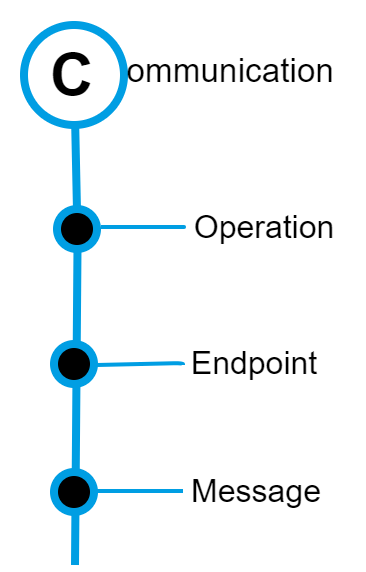
\includegraphics[width=1.36in,height=2.5in]{./media/image39.png}
		\caption{Outline Communication Concern}
		\label{fig:outline_communication_concern}
	\end{Center}
\end{figure}



\subparagraph*{Operation}
%\addcontentsline{toc}{subparagraph}{Operation}
An operation models an atomic unit of functionality in the exchange, processing, visualization, or persistence of digital content. Operations related to each other may be grouped into service interfaces (i.e., sets of a coherent functionality defining an abstract $``$interaction contract$"$ ). 

Example: \textit{Read operation providing access to a parameterized report (may expect a start year parameter, an end year parameter, or both)}. 

\textbf{PARAMETER} Parameters are named slots of an operation’s interface. They define the least level of content granularity an operation may (optional) or must (mandatory) expect as an input or output. Each parameter mediates a particular kind of digital content. This is defined by reusing the triadic content model from Section 3.4.3.5. Thereby abstract aspects (i.e. the meaning) and concrete aspects (i.e. the shape) of the parameter are covered. Optionally, the default value or lists of selectable, enumerated values can be defined as instances of that content model. Additional parameter types (e.g., an ID or the start or end of a period) provide information for operation clients about the purpose and intended usage of the parameter and may e.g. support a query generation process. 

Example: \textit{Parameter indicating a year within the period between 2000 and 2018 (further categorized as the start of a date range)}. 

\textbf{OPERATION TYPE} The type conveys the semantics (i.e., the functional capabilities) of an operation. Building upon conventions established within technology related communities (e.g., REST-architecture paradigm\footnote{https://www.ics.uci.edu/$ \sim $ fielding/pubs/dissertation/rest\_arch\_style.htm }), a taxonomy of operation types (interaction primitives) has been defined for the purpose of Resource exchange, as depicted in \ref{fig:Taxonomy_of_Operation_types_for_Resource_exchange}. 



%%%%%%%%%%%%%%%%%%%% Figure/Image No: 27 starts here %%%%%%%%%%%%%%%%%%%%

\begin{figure}[H]
	\begin{Center}
		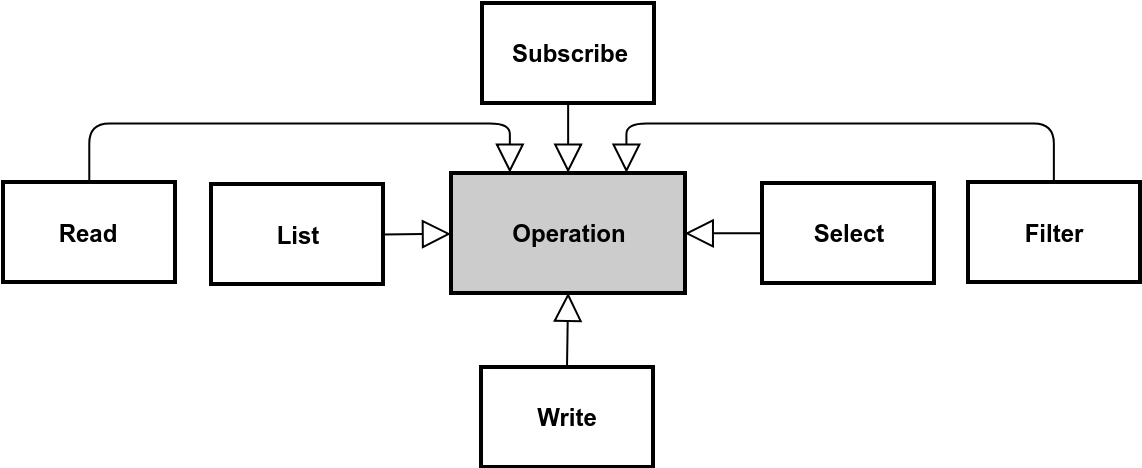
\includegraphics[width=4.15in,height=1.7in]{./media/image40.png}
		\caption{Taxonomy of Operation types for Resource exchange}
		\label{fig:Taxonomy_of_Operation_types_for_Resource_exchange}
	\end{Center}
\end{figure}


%%%%%%%%%%%%%%%%%%%% Figure/Image No: 27 Ends here %%%%%%%%%%%%%%%%%%%%



A client may\textit{ read} the digital content of a single, identified Resource, or \textit{list} a collection of resources. By providing an appropriate expression (e.g., an XPath selector\footnote{https://www.w3.org/TR/xpath-31/ }), the client may \textit{select } a subset of matching resources or \textit{filter } for relevant content fragments (e.g., via an LDAP filter\footnote{https://tools.ietf.org/search/rfc4511$\#$ section-4.5.1 }). The client may \textit{subscribe} for proactive content pushed by the Data Provider, given the permission to \textit{write} (or deliver) the content. Some operation types may impose constraints on type and number of parameters required, as demonstrated by the $``$select$"$  and $``$filter$"$  parameters above.

\textbf{PATTERN }The order of supplying the operation parameters is governed by the operation’s interaction pattern, comparable to web service Message Exchange Patterns\footnote{https://www.w3.org/TR/wsdl20-adjuncts/$\#$ meps } (MEP). For example, the $``$out-only$"$  pattern indicates an unreliable (possibly asynchronous) server-side notification, extended in $``$robust-out-only$"$  pattern by a mandatory confirmation. Such a $``$reliable notification$"$  may be implemented in a variety of ways, depending on the communication protocol and the programming paradigm used.

Example: \textit{In-out interaction pattern, since the result depends on (optional) input parameters}.


%%%%%%%%%%%%%%%%%%%% Figure/Image No: 28 starts here %%%%%%%%%%%%%%%%%%%%

\begin{figure}[H]
	\begin{Center}
		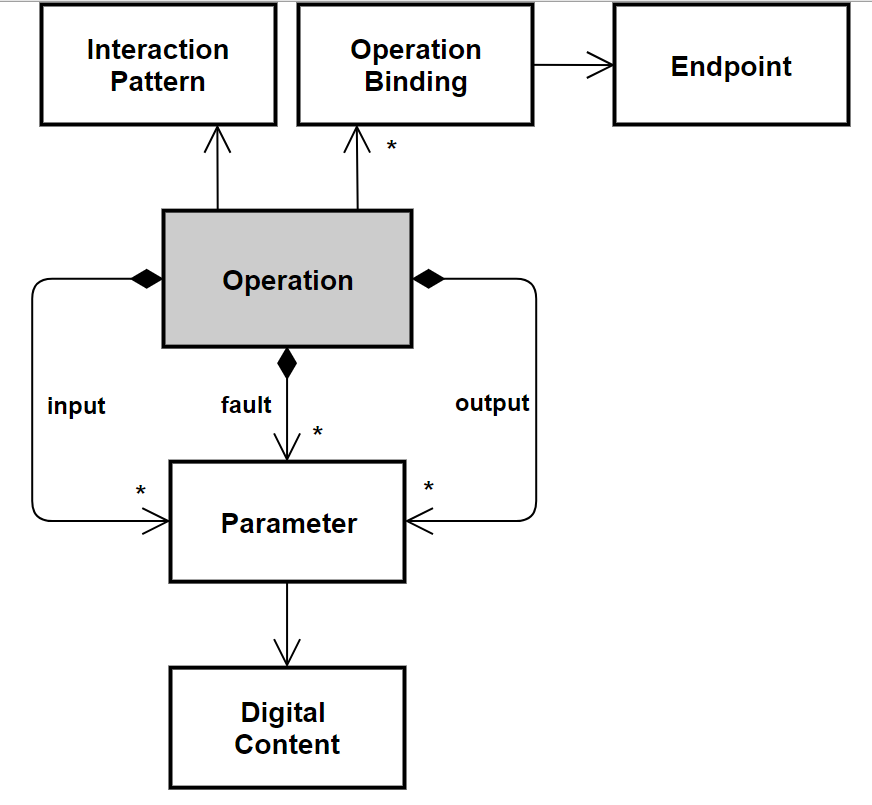
\includegraphics[width=3.08in,height=2.84in]{./media/image41.png}
		\caption{Operation concept (outline)}
		\label{fig:Operation_concept_outline}
	\end{Center}
\end{figure}


%%%%%%%%%%%%%%%%%%%% Figure/Image No: 28 Ends here %%%%%%%%%%%%%%%%%%%%


\subparagraph*{Endpoint}
%\addcontentsline{toc}{subparagraph}{Endpoint}
An Endpoint is a concrete point of content exchange (Resource Endpoint) and service interaction (Service Endpoint) that is uniquely identifiable via a specific communication protocol.

Example: \textit{https://stathub.org/report?start=$ \{ $ year1$ \} $ $\&$ end=$ \{ $ year2$ \} $ }.

\textbf{BINDING }An individual operation or an entire interface can be invoked at an Endpoint by bindings to communication protocols (such as HTTP/2\footnote{https://tools.ietf.org/html/rfc7540 }) by means of established, machine-readable interface description languages (e.g., Open API\footnote{https://www.openapis.org/ }).

\textbf{HOST }The address scheme type (e.g., HTTPS URL, MQTT topic) and communication protocol are defined by the implementing host, which is a server node installed within a Connector. Within the address space of the host, each Endpoint is registered at a particular path, topic, or queue. 

\subparagraph*{Message}
%\addcontentsline{toc}{subparagraph}{Message}
In contrast to the general communication capabilities described above, the Message concept describes the content payload being exchanged at runtime between Connectors. Message metadata provides traceable evidence of the communication (e.g. addresses, transaction ID) and allows interpretation of the context (i.e. type of content, usage contract) within which an Instance of a Resource’s digital content is mediated. Depending on the implementation, this metadata may be supplied as a standalone part of an initial session negotiation or as an integral part of the content transfer (e.g., as header part of a compound multi-part message\footnote{https://tools.ietf.org/html/rfc7578 }). Thus, the Message metadata may either complement interactions of legacy application protocols or may be used independently as a foundation for modeling the exchange of the Resource in a generic, technology-agnostic manner. In the latter case, each state of the interaction is mapped onto an instance of an appropriate Message type (ArtifactRequestMessage). 

Example:\  \textit{Message of the $``$ArtifactRequestMessage$"$  type requesting provision of the artifact named $``$Report\_2000-2010.pdf$"$ }. 

\textbf{MESSAGE TYPE }\textbf{Fehler! Verweisquelle konnte nicht gefunden werden.} illustrates an excerpt of the Message taxonomy. Request-response interactions between the Connectors of interacting participants are reflected by the dedicated subclasses of the RequestMessage and the RequestResponse type. Event-like notifications are reflected by the NotificationMessage subclasses.



%%%%%%%%%%%%%%%%%%%% Figure/Image No: 29 starts here %%%%%%%%%%%%%%%%%%%%

\begin{figure}[H]
	\begin{Center}
		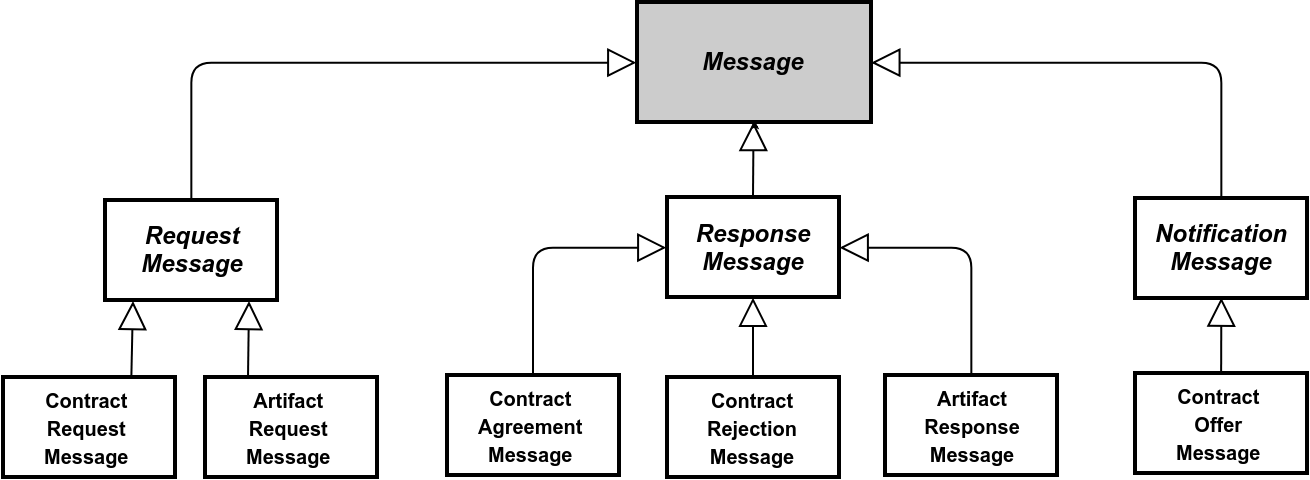
\includegraphics[width=4.5in,height=1.65in]{./media/image42.png}
		\caption{Message taxonomy (excerpt)}
		\label{fig:Message_taxonomy_excerpt}
	\end{Center}
\end{figure}


%%%%%%%%%%%%%%%%%%%% Figure/Image No: 29 Ends here %%%%%%%%%%%%%%%%%%%%


\textbf{ADDRESSING }The Message identifies the participants involved in the interaction (e.g. a Data Provider and a Data Consumer), as well as their Connectors, allowing for routing, provenance tracking, and clearing, among other things.

\textbf{SECURITY} The Security aspect covers, among other things, the authorization features of the client (e.g., JSON Web token\footnote{https://jwt.io/ }) and references to the contract underlying the interaction. 

\paragraph{Commodity\\}
%\addcontentsline{toc}{paragraph}{Commodity}


The \textit{Commodity} concern helps assess the value and utility of a Resource as an obtainable asset with regard to a client’s needs. It addresses questions like:
 \begin{itemize}
	\item Does the Resource originate from a reliable source? 
 	\item What level of quality does the Resource have? 
 	\item What are the restrictions regarding the use of the Resource? 
 	\item How much does it cost to use the Resource?
\end{itemize} 
 \textit{Provenance} explicates the context of the Resource’s creation and its history of modification. The \textit{Quality} of a Resource’s content and provisioning services may be assessed by means of tests, quality of service (QoS) parameters, and ratings from previous users in the community. The \textit{Policy }determines the conditions for using the Resource, including \textit{Pricing}, in a formal way supporting contract negotiation and (automated) contract enforcement. 

\begin{figure}[H]
	\begin{Center}
		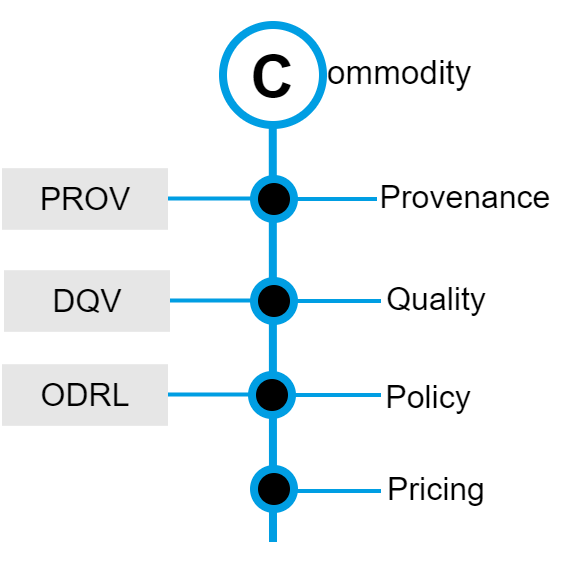
\includegraphics[width=1.34in,height=2.33in]{./media/image43.png}
		\caption{Outline Commodity Concern}
		\label{fig:outline_commodity_concern}
	\end{Center}
\end{figure}


\subparagraph*{Provenance}
%\addcontentsline{toc}{subparagraph}{Provenance}
Provenance is concerned with the origin of the digital content, the history of modifications it has undergone, and the agents responsible for these activities. The main goal of provenance tracking is to ensure reliability of the content, so that modifications are made explicit and comprehensible and may be analyzed for defects. Furthermore, provenance information should refer to the socio-economical context of the content’s creation (the project the content was created in, who the project was funded by etc.) in order to assess the underlying motivation, potential limitations, or bias. 

Example: \textit{Report v3.1, derived from v3.0, including additional tables and diagrams added by John Doe on January 17, 2018}.



\textbf{AGENT} An Agent is any organization, person, or software that has conducted or influenced an Activity. Agents are not necessarily registered participants of the International Data Spaces. Precautions should be taken to ensure a sufficient description of such external Agents is supplied.

\textbf{ACTIVITY} An Activity is a notable, temporarily limited operation applied by an Agent upon the content in question (such as content creation, transformation, usage, or sharing). The vocabulary of Provenance Activities should be controlled (i.e. guidance should be provided to ensure homogeneous annotation and evaluation/querying).


\textbf{CONTENT} The IDS provenance model reuses the generic provenance model of the PROV Ontology\footnote{ https://www.w3.org/TR/prov-o/ } but focuses on uniquely identifiable digital content as a subject to Activities along the Provenance tracking. Depending on the type of Activity, this may link to abstract content (creation), concrete content (specification), or materialized content (modification). 



%%%%%%%%%%%%%%%%%%%% Figure/Image No: 30 starts here %%%%%%%%%%%%%%%%%%%%

\begin{figure}[H]
	\begin{Center}
		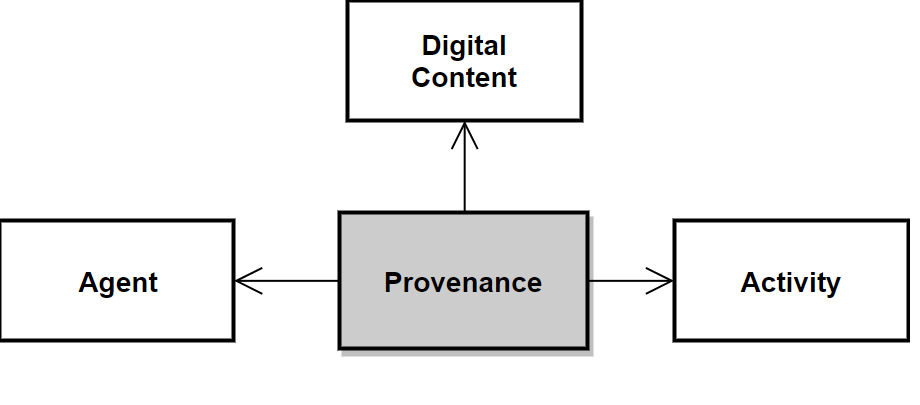
\includegraphics[width=3.74in,height=1.65in]{./media/image44.png}
		\caption{Provenance concept (outline)}
		\label{fig:Provenance_concept_outline}
	\end{Center}
\end{figure}


%%%%%%%%%%%%%%%%%%%% Figure/Image No: 30 Ends here %%%%%%%%%%%%%%%%%%%%


\subparagraph*{Quality}
%\addcontentsline{toc}{subparagraph}{Quality}
Quality is commonly interpreted as $``$fitness for use$"$  (J. M. Juran)\footnote{Juran, J.M., Juran on Planning for Quality. 1988, New York: The Free Press.  }, emphasizing the contextual nature of quality. Data Consumers can assess the fitness of a data offering for their needs based on quality statements supplied alongside with the Resource. These are, among other things, quality assessments according to a multidimensional model (e.g. the ISO/IEC 25012 data quality model\footnote{https://iso25000.com/index.php/en/iso-25000-standards/iso-25012 }, of which the Data Quality Vocabulary (DQV\footnote{https://www.w3.org/TR/vocab-dqv/ }) enables a declarative implementation), a certificate of quality, or any form of community feedback.


\textbf{DIMENSION} A quality Dimension is a qualitative characteristic of a dataset relevant to the Data Consumer. It relates to whether data is complete, valid, accurate, up to date, (technically) available, and so on. User-oriented quality dimensions are measured by means of one or more quantifiable metrics. 

\textbf{METRIC} A quality Metric implements a particular approach to assessing a data quality dimension by observing a concrete indicator, such as the spatial resolution (accuracy) or the up-time of the Resource’s server (availability). The value of a metric is often numeric (percentage) or boolean. 

\textbf{MEASUREMENT} Evaluation of a given dataset against a specific quality metric results in a measurement. Measurement results, as well as individual, subjective assessments may be annotated by means of metadata. 

\textbf{METADATA} Quality related metadata provides provenance information, information about the agent that performed the overall evaluation or an individual measurement (quality checker), information about the source it was originally derived from (accumulative metrics), and the time of evaluation.

\textbf{CERTIFICATE} A quality Certificate is a document that certifies the quality of a Resource according to a set of quality assessment rules, such as the ODI Quality Certificate\footnote{https://certificates.theodi.org/ }. 

\textbf{FEEDBACK }The Feedback comprises any kind of community feedback regarding experiences made with certain data (such as star ratings, issue reports, or recommendations). Feedback considerably affects the credibility of data.



%%%%%%%%%%%%%%%%%%%% Figure/Image No: 31 starts here %%%%%%%%%%%%%%%%%%%%

\begin{figure}[H]
	\begin{Center}
		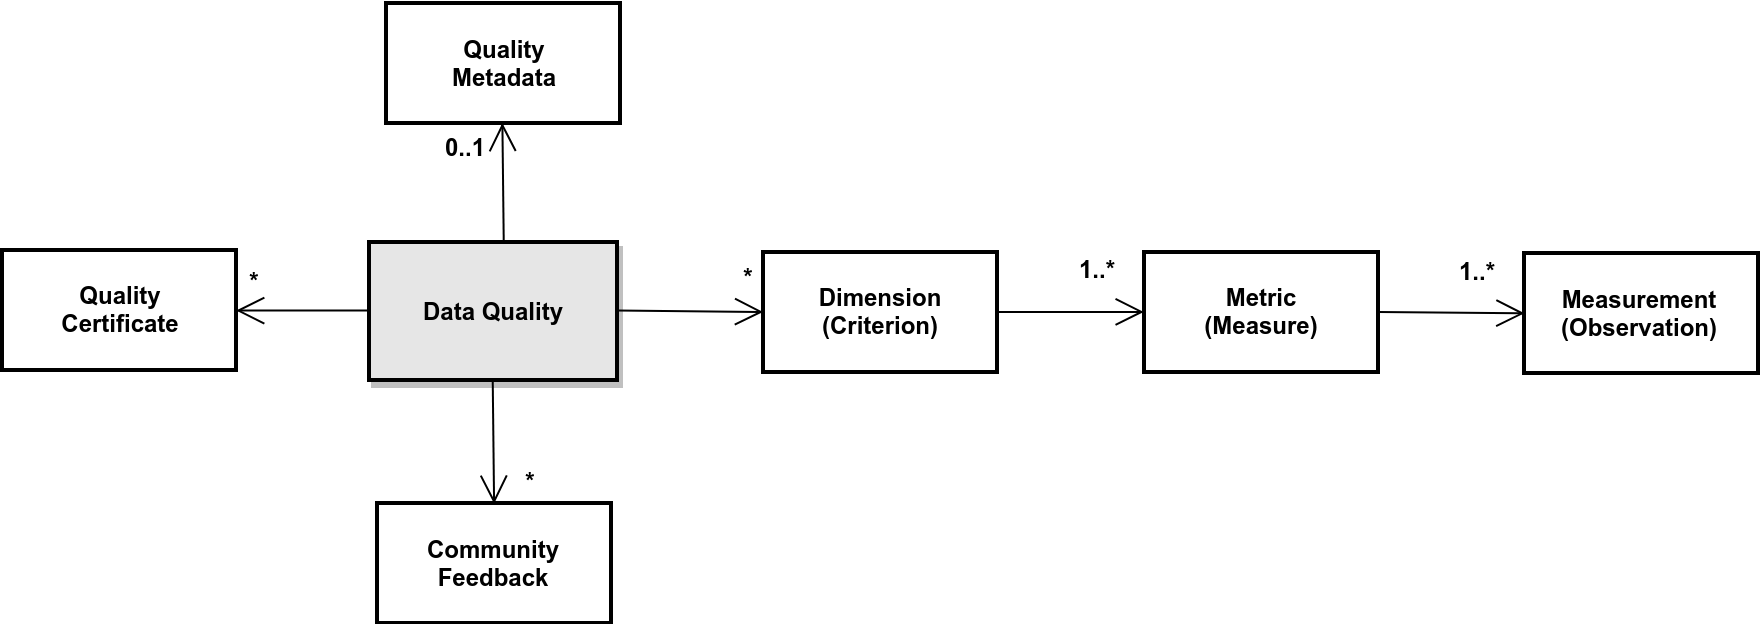
\includegraphics[width=6.53in,height=2.31in]{./media/image45.png}
		\caption{Outline of the: Data Quality concept (outline)}
		\label{fig:Outline_of_the_Data_Quality_concept_outline}
	\end{Center}
\end{figure}


%%%%%%%%%%%%%%%%%%%% Figure/Image No: 31 Ends here %%%%%%%%%%%%%%%%%%%%




\subparagraph*{Policy}
%\addcontentsline{toc}{subparagraph}{Policy}
A Policy defines rules for access to and usage of Resources, as further specified in the subsections on Data Access Control and Data Usage Control of section 4.1.3.
% ToDo: referer
Published as part of a Resource’s metadata using an extension of the Open Digital Rights Language (ODRL)\footnote{ R. Iannella, S. Guth, D. Paehler and A. Kasten, "ODRL Version 2.1 Core Model," 05 03 2015. [Online]. Available: https://www.w3.org/community/odrl/model/2.1/.}, it constitutes a contract offer to be further negotiated and agreed upon by the prospective Data Consumer. 

Example: \textit{Permission for unrestricted usage of report data given the obligation the assignee John Doe will cite the source of data (Creative Commons Attribution, CC-BY)}.

\textbf{RULE} A Rule defines Actions that an involved Party is obliged (Duty), permitted (Permission) or prohibited (Prohibition) to do with respect to an Asset.

\textbf{PARTY }The Parties involved in a data exchange transaction (i.e. the Data Owner/Provider and the Data Consumer, or their representative agents) are referred to by their respective roles, assigner and assignee. 

\textbf{ACTION} Alongside with operations on Assets (e.g. copy, print, convert), an Action may comprise general obligations (e.g. pay, attribute) or modify the interpretation of the policy (e.g. ensure exclusiveness)\footnote{https://www.w3.org/TR/odrl-vocab/$\#$ actionConcepts }. 

\textbf{ASSET }An Asset, i.e., a Resource or a collection of Resources, is the subject of a Rule. Depending on the Policy’s specifications (e.g. do not redistribute), the Asset’s content needs to be identified in a persistent and unambiguous manner in order to be effectively enforceable, independently of the provisioning type (e.g. download URL) or storage context (Data Provider or Data Consumer) (for example, by an identifier composed of indicators such as artifact name and hash sum).

\textbf{CONSTRAINT} A formal Constraint may restrict the applicability of a Rule (e.g. by purpose of use), guide the selection of collection items (e.g. according to the file format) and permissible Parties (e.g. by role), or refine the interpretation of Actions (e.g. print at low resolution). The underlying Policy language has to define appropriate properties (e.g. purpose, file format, role, or resolution) along with conditions of their applicability and interpretation\footnote{https://www.w3.org/TR/odrl-vocab/$\#$ term-LeftOperand }. Reusing quality metrics (e.g. server uptime), as introduced above, allows specifying Policies on the required quality of service (QoS). 



%%%%%%%%%%%%%%%%%%%% Figure/Image No: 32 starts here %%%%%%%%%%%%%%%%%%%%

\begin{figure}[H]
	\begin{Center}
		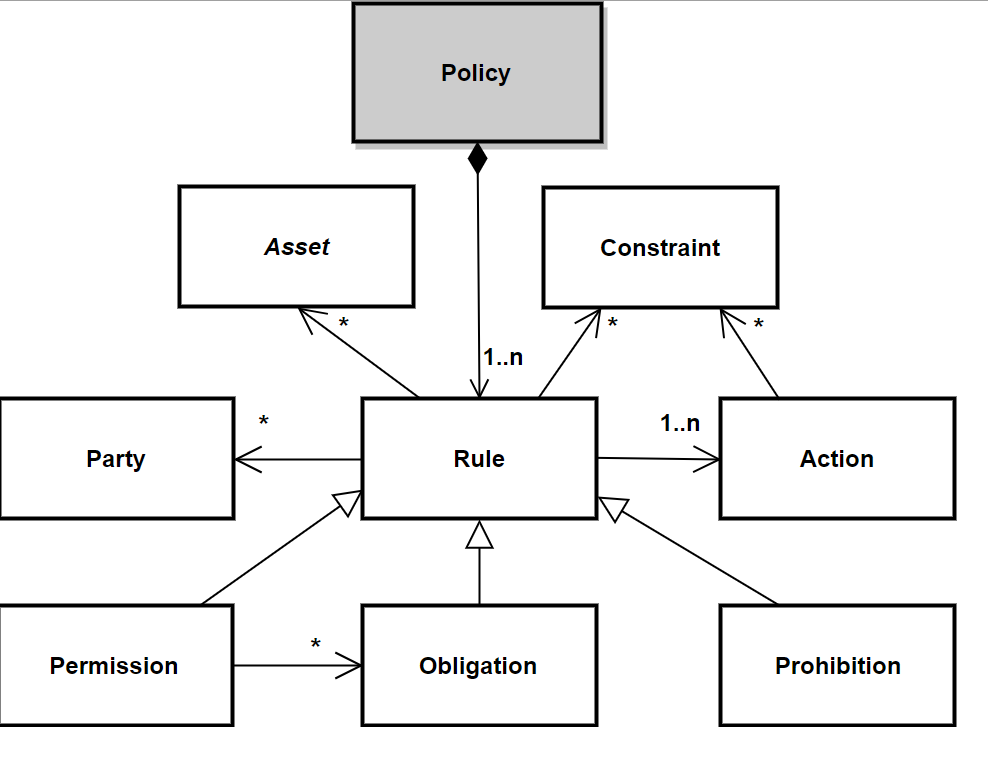
\includegraphics[width=4.14in,height=3.22in]{./media/image46.png}
		\caption{Policy concept (outline)}
		\label{fig:Policy_concept_outline}
	\end{Center}
\end{figure}


%%%%%%%%%%%%%%%%%%%% Figure/Image No: 32 Ends here %%%%%%%%%%%%%%%%%%%%



\subparagraph*{Pricing}
%\addcontentsline{toc}{subparagraph}{Pricing}
Pricing models applied to Resources exchanged in the International Data Spaces may vary. Applying a \textit{Free Use }model, the use of Resources is not charged (while other obligations may still apply, e.g. attribution). The \textit{Freemium} model exposes limited parts (or capabilities) of a Resource at no cost, while for additional parts particular subtypes of \textit{Chargeable Use} apply. The \textit{Quantity-based Pricing} model relies on particular quantitative metrics (e.g. volume, access count, download) to define a charged instance of usage (i.e. pay-per-use). The \textit{Feature-based Pricing} model depends on a selection of content features and quality parameters, such as map layers (basic, mobility, crime), image or audio resolution (low, high) etc. The least restrictive Pricing model, the \textit{Flatrate} model, allows unconstrained use of a Resource at a fixed price, but can potentially be limited by quantitative boundaries (such as bandwidth, number of parallel requests, or data transfer speed).

 Example: \textit{The European highway utilization report is provided free of charge}.


%%%%%%%%%%%%%%%%%%%% Figure/Image No: 33 starts here %%%%%%%%%%%%%%%%%%%%

\begin{figure}[H]
	\begin{Center}
		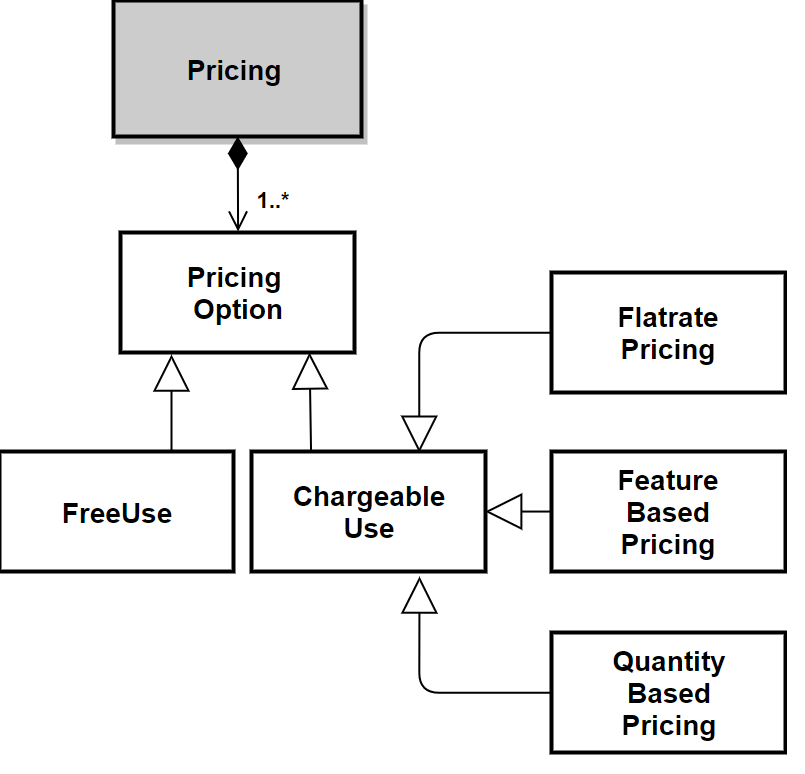
\includegraphics[width=2.7in,height=2.6in]{./media/image47.png}
		\caption{Pricing concept (outline)}
		\label{fig:Pricing_concept_outline}
	\end{Center}
\end{figure}


%%%%%%%%%%%%%%%%%%%% Figure/Image No: 33 Ends here %%%%%%%%%%%%%%%%%%%%



\paragraph{Community of trust\\}
%\addcontentsline{toc}{paragraph}{Community of trust}
The \textit{Community of trust} concern considers the fundamental requirement of the International Data Spaces for exchanging and sharing digital content between a Data Provider and a Data Consumer in a secure and trusted way, while preserving data sovereignty of the Data Owner. It addresses questions like: 
 \begin{itemize}
	\item What is known about the respective counterpart of the intended data exchange transaction? 
 	\item Is the respective system reliable with regard to technical guarantees? 
 	\item Is there a formal proof of the above, e.g. a valid certification? 
 	\item What are the restrictions regarding the use of the acquired content?
\end{itemize} 
 \textit{Participants }registered with the IDS provide or consume digital content by means of a dedicated software component: the \textit{Connector. }Participants and Connectors may undergo a formal \textit{Certification }process (depending on the role a Participant wants to assume in the IDS), stating their trustworthiness according to the criteria catalog and the extent of applied evaluation. Finally, the technical and legal terms of providing and consuming digital content are laid down in a formal \textit{Contract}.


\begin{figure}[H]
	\begin{Center}
		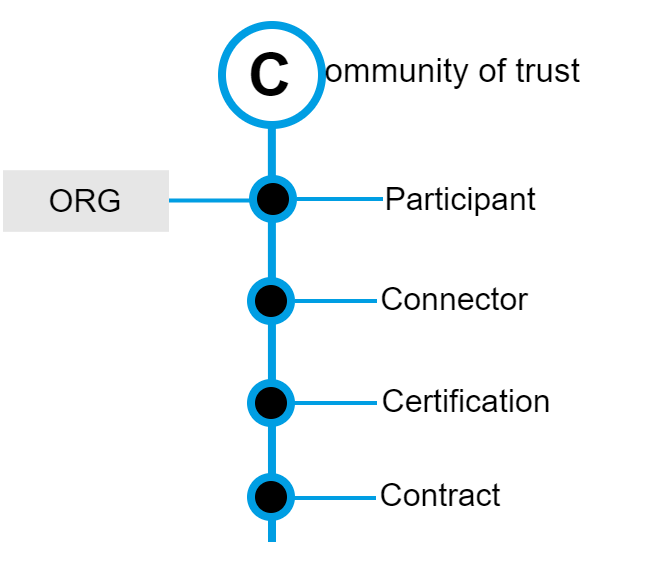
\includegraphics[width=1.36in,height=2.12in]{./media/image48.png}
		\caption{Outline Community of trust Concern}
		\label{fig:community_of_trust_concern}
	\end{Center}
\end{figure}


\subparagraph*{Participant}
%\addcontentsline{toc}{subparagraph}{Participant}
A Participant is a legal or natural person assuming a role (or more than one role) in the International Data Spaces. Participants must undergo a formal certification process.  

Example: \textit{AAStat, a public agency maintaining an infrastructure for monitoring, analysis, and prediction of highway statistics in Germany, has branches in Bonn and Berlin; since it provides open data that is available without any liability, it has refrained from undergoing an expensive certification process}.

\textbf{IDENTITY} Participants are registered at the International Data Spaces with a digital identity (X.509 certificate) issued by an Identity Provider as explained in section 3.1.3,
% ToDo: referer
alongside with other established, external identifiers (such as the D-U-N-S Number\footnote{https://www.dnb.com/duns-number/ }). In accordance with the Linked Data principles, a Participant should always be unambiguously identifiable by a resolvable HTTPS URL, which links to a live metadata document describing the Participant.

\textbf{STRUCTURE} Organizations may link to individual employees, departments, or subsidiaries in order to allow for sharing authorizations, corporate policies etc. across the International Data Spaces.\footnote{See, e.g., the Organization Ontology (ORG) at https://www.w3.org/TR/vocab-org/.}

\textbf{SITE} Each Participant is associated with at least one site that serves the purpose of addressing geo-spatial queries (for reasons of proximity) or finding out about the local law in force. 

\textbf{BUSINESS} Participants may indicate the type of business and the domain in which they operate by making references to an established business classification (such as NAICS\footnote{https://www.census.gov/cgi-bin/sssd/naics/naicsrch?chart=2017 } or ISIC\footnote{https://unstats.un.org/unsd/publication/seriesm/seriesm\_4rev4e.pdf }). This information may support clients searching for digital content by business category. 

\textbf{CERTIFICATION} Depending on the role a Participant wants to assume in the IDS, the Participant may choose (or be required) to undergo an evaluation process resulting in a certification that states its compliance with a criteria catalog based on an evaluation method.



%%%%%%%%%%%%%%%%%%%% Figure/Image No: 34 starts here %%%%%%%%%%%%%%%%%%%%

\begin{figure}[H]
	\begin{Center}
		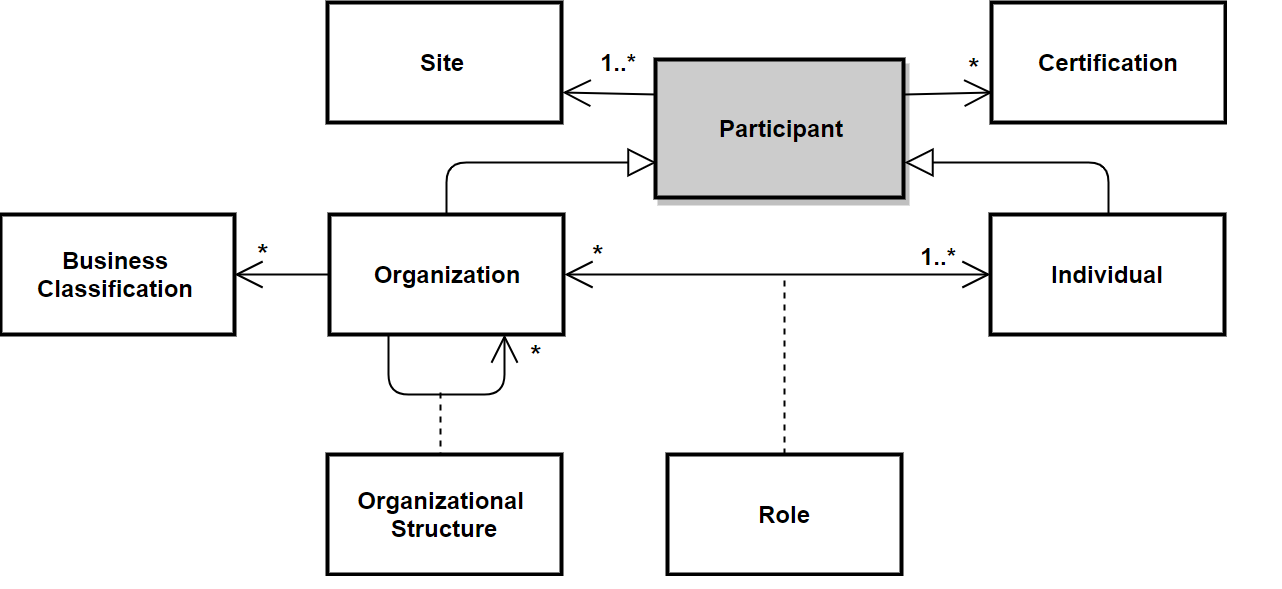
\includegraphics[width=4.68in,height=2.15in]{./media/image49.png}
		\caption{Participant concept (outline)}
		\label{fig:Participant_concept_outline}
	\end{Center}
\end{figure}


%%%%%%%%%%%%%%%%%%%% Figure/Image No: 34 Ends here %%%%%%%%%%%%%%%%%%%%

\subparagraph*{Connector}
%\addcontentsline{toc}{subparagraph}{Connector}
The Connector is the central technological building block of the International Data Spaces. It is a dedicated software component allowing Participants to exchange, share and process digital content. At the same time, the Connector ensures that the data sovereignty of the Data Owner is always guaranteed. Depending on the type of configuration, the Connector’s tamper-proof runtime hosts a variety of system services ensuring, for example, secure bidirectional communication, enforcement of content usage policies, system monitoring, and logging of content transactions for clearing purposes. The functional range of a generic Connector may be extended by custom software (Data Apps), allowing data processing, visualization, persistence etc. 

Roles belonging to the Intermediary category are based on the Connector technology. For example, the Broker Service Provider receives and provides metadata and maintains a metadata registry, the App Store provides Data Apps, and the Vocabulary Hub provides shared vocabularies and related (schema) documents. 

Example: \textit{A Base Connector operated by AAStat at coordinates: 50$ ^{\circ} $ 45'44.6"N 7$ ^{\circ} $ 02'01.2"E. It provides an HTTPS 2.0 host serving traffic sensor data. The Connector has limited capabilities only (IoT device) and holds a base certification level}. 

\textbf{DEPLOYMENT CONTEXT }The Deployment Context of a Connector records, among other things, the Connector’s location (e.g. the data center, coordinates), the type of its deployment (on-premises or cloud-based), and the name of the Participant it is operated by (i.e. the Service Provider). Depending on the policy, this information may affect context-based routing of content. 

\textbf{SECURITY PROFILE} The Security Profile indicates the capabilities of a Connector to maintain a controlled, secure and trusted environment for exchanging, sharing and processing digital content in terms of properties (such as remote integrity verification, application isolation, usage control support, etc.). A counterpart in the data exchange may evaluate this information, alongside with the level of Certification, in order to assess the Connector’s technical trustworthiness. 

\textbf{CATALOG} Connectors may expose an arbitrary number of Resources that provide or consume digital content. The Catalog comprises a metadata model of those Resources constructed in accordance with the IDS Vocabulary. Optionally, the Catalog, or individual sets of Resource metadata, may be advertised via intermediary nodes (such as the Broker Service Provider or the App Store Provider).

\textbf{HOST} Each Host represents an individual communication capability of the Connector, a server that exposes Resources via Endpoints (HTTPS URLs, MQTT topics, etc.) according to the communication protocol supported.



%%%%%%%%%%%%%%%%%%%% Figure/Image No: 35 starts here %%%%%%%%%%%%%%%%%%%%

\begin{figure}[H]
	\begin{Center}
		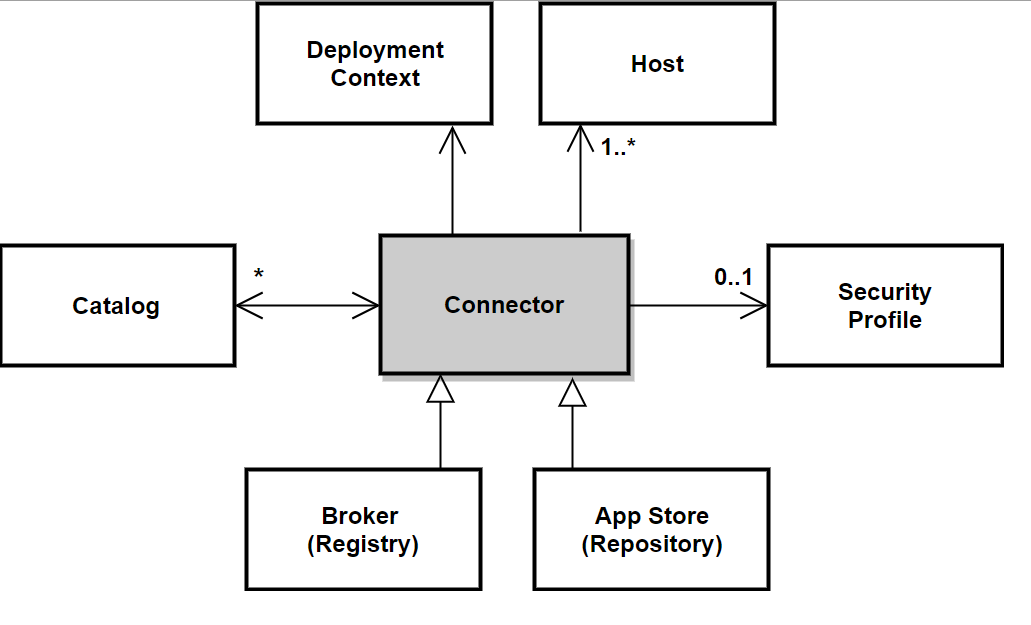
\includegraphics[width=3.92in,height=2.38in]{./media/image50.png}
		\caption{Connector concept (outline)}
		\label{fig:Connector_concept_outline}
	\end{Center}
\end{figure}


%%%%%%%%%%%%%%%%%%%% Figure/Image No: 35 Ends here %%%%%%%%%%%%%%%%%%%%


\subparagraph*{Certification}
%\addcontentsline{toc}{subparagraph}{Certification}
\textit{Certification} aims at determining and formally stating compliance of a Participant or an infrastructure component (basically the Connector) with a predefined set of evaluation criteria. 

Example: \textit{Basic Component Certification based on a self-assessment}.

\textbf{EVALUATION FACILITY }An \textit{Evaluation Facility} carries out the evaluation part during a Participant Certification process, It issues the corresponding Certifications of compliance according to the given \textit{Certification Scheme} (i.e. the processes, roles, evaluation methods, and target criteria). Appointed by the International Data Spaces Association, the \textit{Certification Body }oversees the certification process, defines standardized evaluation procedures, and supervises all activities of the Evaluation Facilities. 

\textbf{CERTIFICATION LEVEL} A successfully completed Certification process results in the assignment of a predefined \textit{Certification Level}, based on a combination of an underlying set of criteria and the depth of the evaluation method chosen. Here, a $``$higher$"$  Certification Level transitively subsumes $``$lower$"$  levels allowing for queries based on a least required level. Certification information is stored in the Participant’s metadata description and attached to the attributes of the X.509 certificate, along with its Validity Period. Certification is expected to be automatically revoked after that date, unless it has been reasserted. 



%%%%%%%%%%%%%%%%%%%% Figure/Image No: 36 starts here %%%%%%%%%%%%%%%%%%%%

\begin{figure}[H]
	\begin{Center}
		\includegraphics[width=4.5in,height=1.81in]{./media/image51.png}
		\caption{Certification concept (outline)}
		\label{fig:Certification_concept_outline}
	\end{Center}
\end{figure}


%%%%%%%%%%%%%%%%%%%% Figure/Image No: 36 Ends here %%%%%%%%%%%%%%%%%%%%

\subparagraph*{(Usage) Contract}
%\addcontentsline{toc}{subparagraph}{(Usage) Contract}
A Usage Contract formalizes the expectations regarding the behavior of Participants involved in a data exchange transaction in a declarative, technology-agnostic way. It constitutes a unique, binding agreement between the Parties on Resource usage conditions as a result of an (automated) negotiation process. Digital Usage Contracts are to be maintained in a safe, unforgeable manner (e.g. blockchain). They are the foundation for clearing and configuring the Resource’s \textit{access control} policies, and for perpetual evaluation and \textit{enforcement }by Usage Control Frameworks, like MYDATA Control\footnote{https://www.mydata-control.de/ }. 

Example: \textit{Agreement between the Data Consumer YourCargo and Data Provider AAStat valid from March 1, 2019 till December 31, 2019 to provide push notifications about delays and traffic obstructions at some enumerated routes. First 5000 messages are free of charge, the remaining are charged on quantity base (5€/1000 messages).}

\textbf{RESOURCE} Usage Policies (cf. section 4.1.3.6.3.1% ToDo: referer
) originally published alongside with a Resource (Contract Offer) are the starting point of a Contract negotiation process. Over the course of this process, any incomplete or newly agreed details regarding Resource exchange are complemented, such as the identification of the Resource content in question, communication Endpoints, authorization token(s), or the provisioning period. 

\textbf{RULE} Likewise, applicable Rules are selected and configured in accordance with the Data Provider’s demand and the Data Consumer’s economic, legal and technical options. By agreeing on a Usage Contract, the Data Consumer explicitly confirms its capability of implementing and enforcing the stipulated rules.



%%%%%%%%%%%%%%%%%%%% Figure/Image No: 37 starts here %%%%%%%%%%%%%%%%%%%%

\begin{figure}[H]
	\begin{Center}
		\includegraphics[width=4.67in,height=2.55in]{./media/image52.png}
		\caption{Usage Contract concept (outline)}
		\label{fig:Usage_Contract_concept_outline}
	\end{Center}
\end{figure}


%%%%%%%%%%%%%%%%%%%% Figure/Image No: 37 Ends here %%%%%%%%%%%%%%%%%%%%

\paragraph{Summary\\}
%\addcontentsline{toc}{paragraph}{Summary}
The previous section introduced the Conceptual Representation of the Information Model with the help of the concern hexagon (C-hexagon). Each corner of the hexagon represents a distinguished concern contributing to the concept of the Digital Resource in the context of the International Data Spaces: 

\begin{itemize}
	\item The \textit{Content} concern deals with the description of a Resource’s inherent substance, i.e. its $``$content$"$  available in any machine-interpretable, binary format. 

	\item The \textit{Context} concern deals with temporal and spatial aspects as well as with real-world entities a Resource’s content relates to. 

	\item The \textit{Concept} concern deals with the modeling of the meaning, annotation, and interpretation of entities introduced by other Resource concerns such as Content and Context. 

	\item The \textit{Communication} concern deals with means to communicate a Resource’s content in one of the Representations available. 

	\item The \textit{Commodity }concern helps to assess the value and utility of a Resource. 

	\item The \textit{Community of trust} concern considers the fundamental requirement of the International Data Spaces for exchanging and sharing Resources between a Data Provider and a Data Consumer in a secure and trusted way, while preserving the data sovereignty of the Data Owner.

\end{itemize}

The main aspects covered by the six concerns are summarized in Figure \ref{fig:Detailed_concern_hexagon}.

%%%%%%%%%%%%%%%%%%%% Figure/Image No: 38 starts here %%%%%%%%%%%%%%%%%%%%

\begin{figure}[H]
	\begin{Center}
          \includegraphics[width=6.53in,height=5.96in]{./media/image53.png}
		\caption{Detailed concern hexagon}
		\label{fig:Detailed_concern_hexagon}
	\end{Center}
\end{figure}


%%%%%%%%%%%%%%%%%%%% Figure/Image No: 38 Ends here %%%%%%%%%%%%%%%%%%%%


\subsubsection{Vocabularies}
%\addcontentsline{toc}{subsubsection}{Vocabularies}
The IDS expresses its Information Model as an RDF ontology in order to provide unambiguous identifiers and formalized definitions of its concepts and relations. To simplify the integration of the IDS ontology, descriptions directly connected to the respective concepts, as well as links to widely-known concepts of so called upper-level ontologies, provide further explanations. As data exchange between different parties is at the core of the IDS, only a fundamental core vocabulary for data descriptions and data exchange invocations is required for all IDS participants. Domain-specific vocabularies may be used wherever necessary to extend the core concepts and to provide more information on data provided or requested. On the one hand, the Information Model be extended by vocabularies describing (Digital) Resources in domain specific ways. On the other hand, the Information Model itself allows, in the scope of its \textit{Content} concern, for describing domain-specific aspects of the structure and/or semantics of the content of a \textit{Resource} or of one of its \textit{Representation}s by referencing domain-specific vocabularies. Terms from such vocabularies may be referenced and their usage in the content of a Resource/Representation may be expressed, e.g., on the level of the Resource/Representation as a whole (using the VoID Vocabulary of Interlinked Datasets\footnote{https://www.w3.org/TR/void/ }), or in the context of describing table/matrix or graph structures of Data Resources (using the Data Cube Vocabulary\footnote{https://www.w3.org/TR/vocab-data-cube/ } or the SHACL Shapes Constraint Language\footnote{https://www.w3.org/TR/shacl/ }, respectively).

\subsubsection{Data App Interfaces}
%\addcontentsline{toc}{subsubsection}{Data App Interfaces}
Similar to an IDS Connector providing information on its identity, functional range, and interaction capabilities, an IDS Data App provides information about itself according to the IDS Information Model. A description file contains details about the intended usage and purpose of the Data App, the security level, and the licensing model applied. In addition, a Data Provider may describe a Data App with vocabularies outside the core IDS Vocabulary (for instance, domain specific explanations may require further terms and concepts).

The description of Data Apps facilitates the discovery and selection of a Data App in an IDS App Store. Consequently, metadata must contain all necessary information to specify the value proposition and the applicability of the respective Data App. Furthermore, metadata is a fundamental building block for the deployment and composition of several Data Apps inside an IDS Connector. Therefore, all operations have to be defined in terms of input and output parameters, bound protocols, and endpoints. Preconditions and postconditions need to be made explicit, and effects on the environment must be outlined.



 %%%%%%%%%%%%  include section 3.5 System Layer here %%%%%%%%%%%%%%

\subsection{System Layer}
%\addcontentsline{toc}{subsection}{System Layer}
On the System Layer, the roles specified on the Business Layer are mapped onto a concrete data and service architecture in order to meet the requirements specified on the Functional Layer, resulting in what can be considered the technical core of the International Data Spaces.

From the requirements identified on the Functional Layer, three major technical components result:

\begin{itemize}
	\item the Connector,\par

	\item the Broker, and\par

	\item the App Store.
\end{itemize}

How these components interact with each other is depicted in Figure \ref{fig:Interaction_of_technical_components}. 


%%%%%%%%%%%%%%%%%%%% Figure/Image No: 39 starts here %%%%%%%%%%%%%%%%%%%%

\begin{figure}[H]
	\begin{Center}
		\includegraphics[width=5.31in,height=3.12in]{./media/image54.png}
		\caption{Interaction of technical components}
		\label{fig:Interaction_of_technical_components}
	\end{Center}
\end{figure}


%%%%%%%%%%%%%%%%%%%% Figure/Image No: 39 Ends here %%%%%%%%%%%%%%%%%%%%

The Connector, the Broker, and the App Store are supported by four additional components (which are not specific to the International Data Spaces, but specified for the International Data Spaces):

\begin{itemize}
	\item the Identity Provider as defined in the Security Perspective,

	\item the Vocabulary Hub currently as defined outside the IDS,
          %% ToDo: Christoph Lange: I do not understand what "outside the IDS" means here.

	\item the Update Repository (i.e. the source for updates of deployed Connectors) depending on the connectors technology, and

	\item the Trust Repository (i.e. the source for trustworthy software stacks and fingerprints as well as remote attestation checks) as discussed in the Security Perspective.
\end{itemize}

A distributed network like the International Data Spaces relies on the connection of different member nodes where Connectors or other core components are hosted (a Connector comprising one or more Data Endpoints). The Connector is responsible for the exchange of data or as a proxy in the exchange of data, as it executes the complete data exchange process (see Section 3.3.2) from and to the internal data resources and enterprise systems of the participating organizations and the International Data Spaces. It provides metadata to the Broker as specified in the connector self-description, e.g. technical interface description, authentication mechanism, exposed data sources, and associated data usage policies. It is important to note that the data is transferred between the Connectors of the Data Provider and the Data Consumer (peer-to-peer network concept).

There may be different types of implementations of the Connector, based on different technologies and depending on what specific functionality is required regarding the purpose of the Connector. Two fundamental variants are the Base Connector and the Trusted Connector (see Section 4.1) as they differ in the capabilities regarding security and data sovereignty.

Connectors can be further distinguished into External Connectors and Internal Connectors:

\begin{itemize}
	\item An External Connector executes the exchange of data between participants of the International Data Spaces. The International Data Spaces network is constituted by the total of its External Connectors. Each External Connector provides data via the Data Endpoints it exposes. Applying this principle, there is no need for a central instance for data storage. An External Connector is typically operated behind a firewall in a specially secured network segment of a participant (so-called $``$Demilitarized Zone$"$ , DMZ). From a DMZ, direct access to internal systems is not possible. It should be possible to reach an External Connector using the standard Internet Protocol (IP), and to operate it in any appropriate environment. A participant may operate multiple External Connectors (e.g., to meet load balancing or data partitioning requirements). External Connectors can be operated on-premises or in a cloud environment.

	\item An Internal Connector is typically operated in an internal company network (i.e., a network which is not accessible from outside). Implementations of Internal Connectors and External Connectors may be identical, as only the purpose and configuration differ. The main task of an Internal Connector is to facilitate access to internal data sources in order to provide data to External Connectors.
\end{itemize}

\subsubsection{Connector Architecture}
%\addcontentsline{toc}{subsubsection}{Connector Architecture}
The Connector Architecture uses application container management technology to ensure an isolated and secure environment for individual data services. A data service matches a system which offers an API to store, access or process data. To ensure privacy of sensitive data, data processing should take place as close to the data source as possible. Any data preprocessing (e.g., filtering, anonymization, or analysis) should be performed by Internal Connectors. Only data intended for being made available to other participants should be made visible through External Connectors.

Data Apps are data services encapsulating data processing and/or data transformation functionality bundled as container images for simple installation by application container management.

Using an integrated index service, the Broker manages the data sources available in the International Data Spaces and supports publication and maintenance of associated metadata. Furthermore, the Broker Index Service supports the search for data resources. Both the App Store and the Broker are based on the Connector architecture (which is described in detail in the following paragraphs) in order to support secure and trusted data exchange with these services.



%%%%%%%%%%%%%%%%%%%% Figure/Image No: 40 starts here %%%%%%%%%%%%%%%%%%%%

\begin{figure}[H]
	\begin{Center}
		\includegraphics[width=6.37in,height=3.34in]{./media/image55.png}
		\caption{Connector Architecture}
		\label{fig:Connector_Architecture}
	\end{Center}
\end{figure}


%%%%%%%%%%%%%%%%%%%% Figure/Image No: 40 Ends here %%%%%%%%%%%%%%%%%%%%


Figure \ref{fig:Connector_Architecture} illustrates the internal structure of the Connector. A concrete installation of a Connector may differ from this structure, as existing components can be modified and optional components added. The components shown in Figure 332 can be assigned to two phases: Execution and Configuration.

The Execution phase of a Connector involves the following components:

\begin{itemize}
	\item \textit{Application Container Management}: In most cases, the deployment of an Execution Core Container and selected Data Services is based on application containers. Data Services are isolated from each other by containers in order to prevent unintended interdependencies. Using Application Container Management, extended control of Data Services and containers can be enforced. During development, and in case of systems with limited resources, Application Container Management can be omitted. Difficulties in container deployment can be handled by special Execution Configurators (see below).

	\item An \textit{Execution Core Container} provides components for interfacing with Data Services and supporting communication (e.g., Data Router or Data Bus to a Connector).

	\begin{itemize}
		\item A \textit{Data Router} handles communication with Data Services to be invoked according to predefined configuration parameters. In this respect, it is responsible of how data is sent (and received) to (and from) the Data Bus from (and to) Data Services. Participants have the option to replace the Data Router component by alternative implementations of various vendors. Differences in configuration can be handled by specialized Execution Configurator plug-ins. If a Connector in a limited or embedded platform consists of a single Data Service or a fixed connection configuration (e.g., on a sensor device), the Data Router can be replaced by a hard-coded software, or the Data Service can be exposed directly. The Data Router invokes relevant components for the enforcement of Usage Policies, e.g. a Policy Enforcement Point (see section 4.1.3.6), as configured in the connector or specified in the Usage Policy.

		\item The \textit{Data Bus} exchanges data with Data Services and Data Bus components of other Connectors. It may also store data within a Connector. Usually, the Data Bus provides the method to exchange data between Connectors. Like the Data Router, the Data Bus can be replaced by alternative implementations in order to meet the requirements of the operator. The selection of an appropriate Data Bus may depend on various aspects (e.g., costs, level of support, throughput rate, quality of documentation, or availability of accessories).

	\end{itemize}

	\item An \textit{App Store Container} is a certified container downloaded from the App Store, providing a specific Data Service to the Connector.

	\item A \textit{Custom Container} provides a self-developed Data Service. Custom containers usually require no certification.

	\item A \textit{Data Service} defines a public API, which is invoked from a Data Router. This API is formally specified in a meta-description that is imported into the configuration model. The tasks to be executed by Data Services may vary. Data Services can be implemented in any programming language and target different runtime environments. Existing components can be reused to simplify migration from other integration platforms.

	\item The \textit{Runtime} of a Data Service depends on the selected technology and programming language. The Runtime together with the Data Service constitutes the main part of a container. Different containers may use different runtimes. What runtimes are available depends only on the base operating system of the host computer. From the runtimes available, a service architect may select the one deemed most suitable.

\end{itemize}

The Configuration phase of a Connector involves the following components:

\begin{itemize}
	\item The \textit{Configuration Manager} constitutes the administrative part of a Connector. Its main task is the management and validation of the Configuration Model, followed by deployment of the Connector. Deployment is delegated to a collection of Execution Configurators by the Configurator Management.

	\item The \textit{Configuration Model} is an extendable domain model for describing the configuration of a Connector. It consists of technology-independent, inter-connected configuration aspects.

	\item \textit{Configurator Management} loads and manages an exchangeable set of Execution Configurators. When a Connector is deployed, the Configurator Management delegates each task to a special Execution Configurator.

	\item \textit{Execution Configurators} are exchangeable plug-ins which execute or translate single aspects of the Configuration Model to a specific technology. The procedure of executing a configuration depends on the technology used. Common examples would be the generation of configuration files or the usage of a configuration API. Using different Execution Configurators, it is possible to adopt new or alternative technologies and integrate them into a Connector. Therefore, every technology (operating system, application container management, etc.) gets its own Execution Configurator.

	\item The \textit{Validator} checks if the Configuration Model complies with self-defined rules and with general rules specified by the International Data Spaces, respectively. Violation of rules can be treated as warnings or errors. If such warnings or errors occur, deployment may fail or be rejected.
\end{itemize}

As the Configuration phase and the Execution phase are separated from each other, it is possible to develop, and later on operate, these components independently of each other. Different Connector implementations may use various kinds of communication and encryption technologies, depending on the requirements given.

\paragraph{Connector Configuration Model\\}
%\addcontentsline{toc}{paragraph}{Connector Configuration Model}
The Connector Configuration Model describes the configuration of a Connector, which is set-up during deployment. The model is technology-independent. A Connector can be configured for different statuses (development, test, or live). 



%%%%%%%%%%%%%%%%%%%% Figure/Image No: 41 starts here %%%%%%%%%%%%%%%%%%%%

\begin{figure}[H]
	\begin{Center}
		\includegraphics[width=6.42in,height=5.37in]{./media/image56.png}
		\caption{Connector Configuration Model}
		\label{fig:Connector_Configuration_Model}
	\end{Center}
\end{figure}


%%%%%%%%%%%%%%%%%%%% Figure/Image No: 41 Ends here %%%%%%%%%%%%%%%%%%%%



The components of the Connector Configuration Model are implemented with the help of special Execution Configurators:


\begin{itemize}
	\item $``$General Information$"$  includes the configuration type, the Connector type (Base, Trusted, Mobile, Embedded, Developer), the Connector version, a timestamp of the last change made to the configuration, the configuration status (development, test, live), and a name of a contact person.

	\item $``$Lifecycle$"$  contains information on the Data Flow, the Service Configuration, and Publishing.

	\begin{itemize}
		\item $``$Data Flow$"$  defines the configuration of tasks and connections established by the Data Router between the Data Services and the Data Bus (for multiple data pipelines).

		\begin{itemize}
			\item $``$Networking$"$  relates to the definition of network parameters (ports, IPs, etc.) for being used inside the Connector as well as for connections to External Connectors.

			\item $``$Security$"$  contains information about, for example, which SSL certificates should be used for connections, or which public key infrastructure should be used.

			\item $``$Compliance / Data Sovereignty$"$  specifies rules to be checked by the Validator before Connector deployment. If warnings or errors occur, deployment may be canceled. This feature is used to prevent incorrect configuration of the Connector.

		\end{itemize}

		\item $``$Service Configuration$"$  defines how configuration parameters for Data Services or other Connector components have to be set.

		\item $``$Metadata$"$  describes the data types for input and output used by different Connector components (see chapter 3.4.5 - App Interfaces). Data Services can provide metadata descriptions, which can be imported to the Configuration Model. This information is used to configure the Data Flow.

		\item $``$Publishing$"$  defines which Data Flows or Data Services are provided to external participants. This information is submitted to a Broker.

		\begin{itemize}
			\item $``$Identity Management$"$  defines the Identity Provider, which is closely integrated with the Connector. To be able to connect to an Identity Provider, a Data Service may need additional libraries.

			\item For $``$Accounting$"$  of a data exchange transaction between participants, it is necessary to record additional information, such as contract specifications, pricing models, or billing details.

			\item $``$Clearing$"$  describes which Clearing House should be informed regarding a certain data exchange transaction.
		\end{itemize}
	\end{itemize}
\end{itemize}


\paragraph{Special Connector Implementations\\}
%\addcontentsline{toc}{paragraph}{Special Connector Implementations}
What type of Connector is to be implemented may depend on various aspects, such as the execution environment given or the current developmental stage regarding Data Services or Data Flows used. In the following, three exemplary scenarios are outlined:

\subparagraph*{Developer Connector}
As is the case for the development of any software, developing Data Services or configuring Data Flows comprises several phases (specification, implementation, debugging, testing, profiling, etc.). For reasons of simplification, it may be useful to run Connectors without application container management. In doing so, the development process can be accelerated, as packing and starting the container can be omitted, and debugging can be done in the development environment. After successfully passing all tests, the configuration model used for the Developer Connector can be used to deploy a productive (live) Connector. Upon deployment in the live environment, the Connector is ready for being used.

\subparagraph*{Mobile Connector}
Mobile operating systems (e.g., Android, iOS, or Windows Mobile) use platforms with limited hardware resources. In such environments, application container management is not necessarily required. The same applies for operating systems which do not support application containers, or systems without any operating system (e.g. microcontrollers). In such environments, Data Services (and the execution core) can be started directly on the host system, without requiring any virtualization. The differences between Connectors \textit{with} containers and Connectors \textit{without} containers can be met by different Execution Configurator modules.

\subparagraph*{Embedded Connector}
Another way of Connector miniaturization offers the Embedded Connector. Embedded Connectors have the same design as Mobile Connectors, and do not necessarily require application container management either. However, unlike Mobile or Developer Connectors, the Configuration Manager is not part of the Connector hardware platform here, which is why remote configuration capabilities of the platform are required (e.g., using an API or configuration files).

Additional steps for Connector miniaturization may include the use of a common runtime for all components, or simplified versions of the Data Router and the Data Bus. If data is to be sent to a fixed recipient only, a simple Data Bus client library may be sufficient. Similarly, it may be sufficient to hard-code a single, fixed connection to the Data Bus instead of using a configurable component. To save communication overhead, simple API calls inside the common runtime could be used.

\subsubsection{Meta Data Broker}
%\addcontentsline{toc}{subsubsection}{Broker}

%old
%The IDS Broker consists of an IDS Connector (see section 3.5.1), a service for data source registration, publication, maintenance, and query, based on an index. Therefore, for any interaction with the IDS Broker the processes defined on the Process Layer, the descriptions defined on the Information Layer, and descriptions defined on the System Layer can be applied. The Information Layer describes the message types for Broker registration and query. An IDS Broker may provide additional services that must be described by the IDS Information Model. 

%new
The IDS Meta Data Broker is a service for publishing and searching metadata of connectors and resources between International Data Spaces Participants. In order to ensure the necessary interoperability and general interactions, an IDS Meta Data Broker is also defined as a specialized IDS Connector. The communication between an IDS Connector and an IDS Meta Data Broker is based on the same principles as any other Connector-Connector communication within the International Data Spaces. Still, an IDS Meta Data Broker provides a collection of additional functionalities:
\begin{itemize}
	\item Indexing services in order to effectively and efficiently respond to queries and present known Connectors and other resources
	\item Interfaces for Users or IDS-Messages to ensure access to the stored information. 
\end{itemize}


The capabilities and functionalities of an IDS Meta Data Broker are subject of IDS Certification. After a successful certification of the relevant Criteria of an IDS Connector and as an IDS Meta Data Broker, a software component can include the following RDF statement into its Self-Description:
 
\begin{verbatim}
<Connector/Broker URI>
<http://www.w3.org/1999/02/22-rdf-syntax-ns#type>
<https://w3id.org/idsa/core/Broker> .
\end{verbatim}
\todo{make a listing with numbering out of this}

In accordance to the thereby directly included guaranteed features, an IDS conform Meta Data Broker may provide significantly more services. Several options to include broker features in an International Data Space are possible: 
\begin{itemize}
	\item only mandatory IDS Meta Data Broker features as specifed in the IDS Meta Data Broker Specification\footnote{ToDo Link},
	\item mandatory and optional features as specifed in the IDS Meta Data Broker Specification,
	\item general features supporting publication, indexing and discovery which are not mentioned in this as specifed in the IDS Meta Data Broker Specification (not applicable as an IDS Meta Data Broker, if they interfere with mandatory features), or
	\item any combination of the first three categories.
\end{itemize}


\subsubsection{Data Apps and App Store}
%\addcontentsline{toc}{subsubsection}{Data Apps and App Store}
As described in section 3.5.1 Connectors can make use of Apps for several purposes. Three types of Data Apps can be distinguished:

\begin{itemize}
	\item self-developed Data Apps, which are used by the Data Provider's own Connector (usually requiring no certification from the Certification Body),

	\item third-party Data Apps, which are retrieved from the App Store (and which may require certification), and

	\item Data Apps provided by the Connector of the Data Consumer, which allow the Data Provider to use certain functions before data is exchanged, e.g., filtering or aggregation of data (which may also require certification).
\end{itemize}

In addition, Data Apps can be divided into three categories:

\begin{itemize}
	\item System Adapters are Data Apps establishing interfaces to external enterprise information systems. The main tasks System Adapters is providing access to enterprise information systems and, if necessary, transforming from an internal data model to a data model applicable for data a exchange (e.g., a standard or recommendation for a given application domain), as well as to enrich the data with the required
	metadata to exchange information with other Connectors. System Adapters can be used by Data Providers and Data Consumers, i.e., for reading and writing data to enterprise information systems. 

	\item Smart Data Apps execute any kind of data processing or transformation. Normally, the data provided by, or sent to, a Smart Data App is already annotated with metadata (as described in the Information Layer section). The important difference to System Adapters is that Smart Data Apps have input \emph{and} output data, as they process the input data to provide value-added
	output data. For example, a Smart Data App could apply a data transformation (e.g., from miles into meters or from XML into JSON) or apply machine learning to do classification (e.g., to recognize malicious
	behavior of a machine).

	\item Management Apps provide additional functionality within a Connector, but do not deal directly with the data being exchanged. For example, Usage Policies can enforce the processing of the data in a trusted environment, i.e., a Trusted Connector. A monitoring app could provide statistical information about data usage to a Data Provider.
\end{itemize}



The IDS App Store is a secure platform for distributing Data Apps and features different search options (e.g., by functional or non-functional properties, pricing model, certification status, community ratings, etc.). An IDS App Store consists of a registry for available Data Apps in this App Store. Therefore, an App Store supports operations for Data App registration, publication, maintenance, and query, as well as operations for the provisioning of a Data App to a connector. These basic operations can be complemented by additional services, e.g., billing or support activities. 

\todo{Hier Verweis auf Jive-Dokument hinzufügen? : https://industrialdataspace.jiveon.com/docs/DOC-2604}


 %%%%%%%%%%%%  include section 4.1 security perspective here %%%%%%%%%%%%%%


\section{Perspectives of the IDS-RAM}
Directly related to the five layers of the IDS-RAM are three cross-sectional perspectives: \textit{Security}, \textit{Certification}, and \textit{Governance}. These are described in detail in the following sections.

\subsection{Security Perspective}
%\addcontentsline{toc}{subsection}{Security Perspective}
As stated in Section 1.1, one strategic requirement of the International Data Spaces is to provide secure data supply chains. This is critical for establishing and maintaining trust among Participants that want to exchange and share data and use Data Apps. The IDS Security Architecture provides means to identify Participants,, protect communication and data exchange transactions, and control the use of data after it has been exchanged.

For these purposes, the International Data Spaces defines a Trusted Connector as an extension of the Base Connector (see Section 3.5). The IDS Connector ensures that the specifications and requirements of the Security Architecture materialize in everyday interactions and operations in the International Data Spaces. The security aspects described in the following constitute the basis of the IDS Connector. The differences between a Trusted Connecter and a Base Connector are detailed in the Security Profiles subsection 4.1.3.3.6.

\subsubsection{Security Aspects Addressed by the Different Layers of the IDS-RAM}
%\addcontentsline{toc}{subsubsection}{Security Aspects Addressed by the Different Layers of the IDS-RAM}

\paragraph*{Business Layer\\}

Security aspects are crucial for the definition of roles and basic interaction patterns in the International Data Spaces.

\paragraph*{Functional Layer\\}

Security requirements may restrict certain transactions or operations in the International Data Spaces, or even prevent them. However, security is also an enabling factor. Without security, many use cases would not be possible (e.g., offering sensitive data to trusted business partners). The concept of data usage control allows Data Providers to attach data usage policy information to their data in order to define how a Data Consumer may use the data.

\paragraph*{Process Layer\\}

To take security aspects into account on the Process Layer, it is important that existing processes are permanently monitored, validated, and redesigned, if need be. For example, to allow trustworthy identification and authentication of Participants using a central public key infrastructure (PKI), a Participant must apply for a public key certificate that is registered in a central PKI and deployed inside its Connector. For dynamic attribute support, an identity management server needs to verify attributes before issuing access tokens. The same is true for trustworthy operations of an App Store, for which data must be verified and signed by a trusted entity before it can be uploaded.

\paragraph*{Information Layer\\}

The Information Layer provides the means for Participants to use a common vocabulary and common semantics to express concepts and relationships between them. In doing so, it is possible to specify access and usage control policies in a way that these are understood by all Participants. The same is true for access control requirements defining minimum security profiles, which must be met before access is granted.

\paragraph*{System Layer\\}

As the Connector is the central technical component on the System Layer, it is predominantly the Connector where the security features of the International Data Spaces are implemented. Being an extension of the Base Connector, the Trusted Connector takes up all relevant security specifications and requirements, and serves as the technological basis for use case implementations.

\subsubsection{General Security Principles}
%\addcontentsline{toc}{subsubsection}{General Security Principles}
The development of the Security Architecture follows two general principles:

\paragraph*{Use of existing standards and consideration of best practices\\}

To the extent possible and reasonable, existing standards and best practices are to be used and leveraged in the development of the Security Architecture. The aim of the Security Architecture is not to offer new solutions for problems already solved, but to combine existing, reliable approaches in a useful and meaningful way, and bridge gaps where necessary.

\paragraph*{Scalability of security levels\\}

The International Data Spaces does not enforce a single level of security to be applied for all Participants. This way, also organizations with limited resources and technical means are able to participate (at least as Data Consumers). However, also the security level of these participants must be reliable and verifiable for others. Certain minimum security requirements (e.g., encrypted communication) therefore need to be met by all Participants.

Provided a Participant is in line with general security requirements, it may decide about the level of security to be applied for it itself. It should be noticed, however, that data sources may presuppose a certain minimum level of security to be met by potential Data Consumers. This means for Data Consumers: the higher the security level they choose for themselves to be applied, the better the access to high-quality data sources and high-value data services.

\subsubsection{Key Security Concepts}
%\addcontentsline{toc}{subsubsection}{Key Security Concepts}
The Security Architecture addresses seven key security concepts: 1) secure communication, 2) identity management, 3) trust management, 4) trusted platform, 5) data access control, 6) data usage control and 7) data provenance tracking. 

\paragraph{Secure Communication\\}
%\addcontentsline{toc}{paragraph}{Secure Communication}
To ensure confidentiality and authenticity of data transfers, communication between Connectors must be protected. When using the IDS Connector, two layers of security are in place:

\begin{itemize}
	\item point-to-point encryption (between Connectors), using an encrypted tunnel, and

	\item end-to-end authorization (authenticity and authorization based on actual communication endpoints; i.e., Data Apps).
\end{itemize}

Data from one External Connector to another is sent over the Internet or via a virtual private network (VPN), the specification of which is beyond the scope of the IDS Security Architecture. The Security Architecture defines the IDS Communication Protocol (IDSCP), which must be supported by Trusted Connectors, and can be supported by any other Connector as well. The purpose of the IDSCP is to establish confidential, authenticated communication, exchange data between the Data Provider and the Data Consumer, and establish mutual remote attestation (if supported by the Connectors involved). IDS Connectors must communicate with each other over an encrypted tunnel (e.g., TLS), as depicted in Figure 41, and may use IDSCP or another appropriate protocol, like https or mqtt.



%%%%%%%%%%%%%%%%%%%% Figure/Image No: 42 starts here %%%%%%%%%%%%%%%%%%%%

\begin{figure}[H]
	\begin{Center}
		\includegraphics[width=6.53in,height=1.18in]{./media/image57.png}
		\caption{ IDS Communication }
		\label{fig:_IDS_Communication_}
	\end{Center}
\end{figure}


%%%%%%%%%%%%%%%%%%%% Figure/Image No: 42 Ends here %%%%%%%%%%%%%%%%%%%%


The IDSCP is a high-level protocol established via WebSocket Secure (WSS). It contains several $``$conversations$"$ , which can be initiated by either side and must be confirmed by the other side to be entered. Currently, two conversations are provided: remote attestation and metadata exchange. The protocol itself is performed inside a tunneled connection.

The protocol supports and enables several communication aspects:

\begin{itemize}
	\item identification and authentication,

	\item remote attestation,

	\item metadata exchange, and

	\item data exchange (together with usage policy information attached).

\end{itemize}

The last aspect, data exchange, provides the basic mechanism of data usage control, as it is possible to attach data usage policy information in order to specify how the data may be used by the Data Consumer. However, the specification of the IDSCP is not part of this document.

\paragraph{Identity Management\\}
%\addcontentsline{toc}{paragraph}{Identity Management}
To be able to make access control related decisions that are based on reliable identities and properties of Participants, a concept for Identity and Access Management (IAM) is mandatory. The following aspects are central for the concept:

\begin{itemize}
	\item identification (i.e., claiming an identity),

	\item authentication (i.e., verifying an identity), and

	\item authorization (i.e., making access decisions based on an identity).
\end{itemize}

The \textit{Certificate} \textit{Authority (CA)} issues certificates for all entities. These certificates are used for authentication and encryption between Connectors.

An identity may have several attributes, which are linked to that identity. A Dynamic Attribute Provisioning Service (DAPS) is used to provide dynamic, up-to-date attribute information about Participants and Connectors.

\subparagraph*{Mapping of Participant Certification and Connector Certification to Identity Management\\}
%\addcontentsline{toc}{subparagraph}{Mapping of Participant Certification and Connector Certification to Identity Management}
There are two targets of certification: Participants (receiving a Participant Certificate) and Core Components (receiving a Core Component Certificate). If a Participant (e.g., a company) is successfully certified, it is allowed to participate in the International Data Spaces. The Participant has to use a certified IDS Connector. With both certificates, the Participant Certificate and the Core Component Certificate, the Participant can request a digital X.509 certificate for identification, authentication, and encryption.

A X.509 certificate contains only the most relevant, static information:

\begin{itemize}
	\item \textbf{C (countryName):} country of the organization (e.g. DE);

	\item \textbf{O (organizationName):} name of the organization (e.g. Fraunhofer); 

	\item \textbf{OU (organizationalUnitName):} name of the organizational unit (e.g. AISEC),

	\item \textbf{CN (commonName):} Universally Unique Identifier (UUID) (e.g. 59C3BAE6-1C06-4723-802B-12C7DCF94E58);


	\item \textbf{subjectAltName (X509v3 Subject Alternative Name):} is filled with DNS entries / IP addresses of the Connector ( e.g.\\
DNS.1 = localhost\\
DNS.2 = idsconnector.aisec.fraunhofer.de\\
IP.1 = 0.0.0.0\\
IP.2 = 10.1.2.15\\
IP.3 = 10.1.2.16\\
IP.4 = 10.1.2.17\\
IP.5 = 10.1.2.18\\
)
\end{itemize}


It is important to note that any modification of attributes leads to revocation and reissuing of the certificate. For this reason, the number of attributes that are contained in a certificate needs to be kept at a minimum. Dynamic attributes are kept by the Dynamic Attribute Provisioning Service (DAPS).

\subparagraph*{Proposed PKI Structure\\}
%\addcontentsline{toc}{subparagraph}{Proposed PKI Structure}
In general, a PKI can have several layers to achieve separation of duties (i.e., every Sub-CA is responsible for a specific topic). Depending on the business and deployment model applied, several Sub-CAs may exist.



%%%%%%%%%%%%%%%%%%%% Figure/Image No: 43 starts here %%%%%%%%%%%%%%%%%%%%

\begin{figure}[H]
	\begin{Center}
		\includegraphics[width=6.53in,height=1.62in]{./media/image58.png}
		\caption{ PKI structure (example)}
		\label{fig:_PKI_structure_example}
	\end{Center}
\end{figure}


%%%%%%%%%%%%%%%%%%%% Figure/Image No: 43 Ends here %%%%%%%%%%%%%%%%%%%%


This allows for specific parties to issue certificates for specific purposes. It is also possible to support multiple instances (e.g., multiple Connector Sub-CAs). The structure of the PKI is not defined in this document.

\subparagraph*{Connector Certificate Deployment\\}
%\addcontentsline{toc}{subparagraph}{Connector Certificate Deployment}
After obtaining the Participant Certificate and a Core Component Certificate, an organization may apply for one or more X.509 Certificates (the issuing of which may be triggered by the International Data Spaces Association, for example).

The attributes for Connectors to be embedded in the X.509 certificate are defined above.

Once received, the Connector Certificate can be deployed onto the Connector.



%%%%%%%%%%%%%%%%%%%% Figure/Image No: 44 starts here %%%%%%%%%%%%%%%%%%%%

\begin{figure}[H]
	\begin{Center}
		\includegraphics[width=6.53in,height=3.29in]{./media/image59.png}
		\caption{ Embedding the Connector Certificate }
		\label{fig:_Embedding_the_Connector_Certificate_}
	\end{Center}
\end{figure}


%%%%%%%%%%%%%%%%%%%% Figure/Image No: 44 Ends here %%%%%%%%%%%%%%%%%%%%


The X.509 Certificate ensures that data is always exchanged in an authenticated and encrypted manner.

\subparagraph*{Using the Dynamic Attribute Provisioning Service (DAPS) for Identity Management \\}
%\addcontentsline{toc}{subparagraph}{Using the Dynamic Attribute Provisioning Service (DAPS) for Identity Management }
Using a service to hand out attributes in a dynamic fashion reduces the need for certificate revocation and enables more flexible attribute handling for participants in the International Data Spaces. This allows dynamic assignment of attributes and status flags to Connector instances. Examples of status flags are:

\begin{itemize}
	\item Withdraw a security status if known vulnerabilities have not been fixed.

	\item Upgrade the certification status without reissuing a X.509 certificate.

	\item Assign membership status to a workflow with contractors.

	\item Notification of temporary changes of a Participant’s level of trustworthiness.

	\item Provisioning of mutable attributes (e.g. address of the organization).

\end{itemize}

This concept avoids revocation of certificates in most cases, as it allows to include new attributes if need arises.

\subparagraph*{Using an Authorization Service for Resource Access Control \\}
%\addcontentsline{toc}{subparagraph}{Using an Authorization Service for Resource Access Control}
Using an Authorization Service (featuring access tokens) allows use case dependent modeling of access control decisions. Delegation of access decisions is possible. In complex workflows, multiple Connectors can use a dedicated Authorization Service to delegate resource access decisions. The DAPS acts as the Authorization Service for the IDS.



%%%%%%%%%%%%%%%%%%%% Figure/Image No: 45 starts here %%%%%%%%%%%%%%%%%%%%

\begin{figure}[H]
	\begin{Center}
		\includegraphics[width=7.36in,height=3.39in]{./media/image60.png}
		\caption{ Resource access workflow}
		\label{fig:_Resource_access_workflow}
	\end{Center}
\end{figure}


%%%%%%%%%%%%%%%%%%%% Figure/Image No: 45 Ends here %%%%%%%%%%%%%%%%%%%%


A workflow for accessing a resource (e.g., a Data Service) using dynamic attributes and access tokens is defined as follows:

\begin{enumerate}[label*=\arabic*.]
	\item A Dynamic Attribute Token (DAT) is requested from the Dynamic Attribute Provisioning Service, presenting the Connector's X.509 certificate. Depending on the verification policy specified, the attribute can be verified at the CA.

	\item Before accessing a resource, a TLS tunnel is established using the same X.509 certificate. Again, depending on the policy specified, the certificate can be verified at the CA.

	\item (Optional) If using several Access Tokens (ATs), a token request is performed at a separate Authorization Service in the domain of a use case operator or the domain of the Connector's (or, more specifically, resource’s) owner.

	\item The resource is requested by handing in either the Dynamic Attribute Token (DAT) or the Access Token (AT).
\end{enumerate}

Due to the small size of access tokens, it is possible to incorporate these tokens into any resource request and support stateless access management. Both DATs and ATs use the JSON Web Token (IETF RFC 7519)\footnote{ https://tools.ietf.org/html/rfc7519 } standard.

\paragraph*{Trust Management \\}
%\addcontentsline{toc}{paragraph}{Trust Management}
To establish trust across the entire business ecosystem (i.e., to protect Participants from fraud and ensure they abide by the designated rules), the International Data Spaces makes use of cryptographic methods. One such method is the public key infrastructure (PKI). A central principle of a PKI is that every entity is allocated with secret keys, allowing each entity to authenticate against other Participants. Thereby, a hierarchy is created, with the Identity Provider on top issuing certificates to the other entities, which in turn may issue certificates to other entities, and so on. In the following, the PKI rollout is described for mapping roles and entities required for the deployment of the International Data Spaces.



%%%%%%%%%%%%%%%%%%%% Figure/Image No: 46 starts here %%%%%%%%%%%%%%%%%%%%

\begin{figure}[H]
	\begin{Center}
		\includegraphics[width=4.85in,height=3.09in]{./media/image61.png}
		\caption{ Technical roles in the International Data Spaces}
		\label{fig:_Technical_roles_in_the_International_Data_Spaces}
	\end{Center}
\end{figure}


%%%%%%%%%%%%%%%%%%%% Figure/Image No: 46 Ends here %%%%%%%%%%%%%%%%%%%%


\subparagraph*{PKI Rollout\\}
%\addcontentsline{toc}{subparagraph}{PKI Rollout}
To guarantee secure identity management, the International Data Spaces defines technical roles for implementing a PKI system that is flexible enough to support all roles defined on the Business Layer. In particular, six entities with different security levels are relevant for the Security Architecture. In the following, these entities and the technical roles related to them are described. 

\subparagraph*{Identity Provider\\}

The Identity Provider acts as an agent for the International Data Spaces Association. It is responsible for issuing technical identities to parties that have been approved to become Participants in the International Data Spaces. The Identity Provider is instructed to issue identities based on approved roles (e.g., App Store or App Provider). Only if equipped with such an identity, an entity is allowed to participate in the International Data Spaces (e.g., to provide data or publish Data Apps). The Identity Provider may exclude Participants from the International Data Spaces, if instructed to do so. 

As a trusted entity, the Identity Provider manages the PKI rollout. It takes care if certificates expire or must be revoked. There are two separate PKI hierarchies: one for software signatures (Software Signing Root CA) and one for the Connectors (Service Root CA). An entity is assigned with either an end certificate or a sub/root-CA certificate. The two hierarchies protect the interests of the six entities.



%%%%%%%%%%%%%%%%%%%% Figure/Image No: 47 starts here %%%%%%%%%%%%%%%%%%%%

\begin{figure}[H]
	\begin{Center}
		\includegraphics[width=4.63in,height=3.55in]{./media/image62.png}
		\caption{ Mapping of technical roles and PKI layout}
		\label{fig:_Mapping_of_technical_roles_and_PKI_layout}
	\end{Center}
\end{figure}


%%%%%%%%%%%%%%%%%%%% Figure/Image No: 47 Ends here %%%%%%%%%%%%%%%%%%%%


\subparagraph*{Software Provider \\}

A Software Provider produces and distributes basic software stacks for Connectors (for rollout and deployment). To every Software Provider seeking admission to the International Data Spaces, the Identity Provider issues a service sub-CA request. An approved Software Provider uses the service sub-CA during rollout and deployment of the Connector in order to provide it with an initial, valid and preconfigured system.

\subparagraph*{Connector \\}

A Connector is allowed to communicate with other Connectors only if acquired from an approved Software Provider. Connectors download Data Apps from the App Store. For each Data App downloaded, the Connector creates a service key pair and a Certificate Signing Request (CSR). While the private key is used to identify the Data App and to protect its data, the CSR is sent to the App Store, which uses it to issue a certificate. This also allows entities to check whether the license of a certain Data App is still valid (see e.g. remote attestation). Furthermore, the private key and the certificate are used for establishing a secure channel with other Connectors. During rollout, the Software Provider deploys an initial system onto the Connector and signs the Connector's corresponding service CSRs for the initial system.

\subparagraph*{App Store \\}

A Connector downloads the software it requires (i.e. Data Apps) from an App Store. Connectors can only connect with the App Store for requesting downloads and updates. As the App Store is a Connector itself, it additionally stores its own sub-CA. When a new provider sets up an App Store, the Identity Provider signs a sub-CA request issued by the App Store provider. The App Store provider deploys this sub-CA inside the App Store (i.e., inside the respective Connector). This sub- CA is used by the App Store to ensure the validity of services downloaded by other Connectors. This means that if an App Store signs a CSR (i.e., issues a certificate), a Connector receives a certificate for a downloaded Data App.

\subparagraph*{App Provider \\}

App Providers must seek approval of Data Apps from the Certification Body. Upon successful certification of a Data App, the App Provider may publish the Data App by uploading it to the App Store. Each App Provider can be unambiguously identified by a certificate issued by the Identity Provider.

\subparagraph*{Certification Body \\}

When an App Provider uploads a Data App, the App Store not only checks if the Data App comes from an approved App Provider, but also if the software meets certain quality and security standards. Therefore, App Providers must send the Data App to a Certification Body for inspection. The Certification Body checks the validity of the App Provider’s signature. If the signature is valid, the source code of the respective Data App is inspected. If the Data App meets the quality and security standards, the Certification Body signs the Data App with the certificate's private key. To do so, it does not need a sub-CA, as it only signs the software, but does not create a certificate.

\subparagraph*{Connector Manifestations \\}
%\addcontentsline{toc}{subparagraph}{Connector Manifestations}
A Connector can run different services and communicate with other Connectors. Using the PKI, a Connector protects the persistent storage of its services and the communication with other Connectors (in terms of authenticity, confidentiality, etc.). The following items characterize a Connector in the International Data Spaces from the security perspective:

\subparagraph*{Configuration \\}

Among other things, the configuration specifies from where the Connector downloads new services, or which Brokers or Online Certificate Status Protocol (OCSP)\footnote{ https://tools.ietf.org/html/rfc6960 } servers it uses. Configuration is required in order to boot the system. It is executed during the Connector’s deployment.

\subparagraph*{CA Certificates \\}

In order to verify PKI signatures (e.g., for authentication or for Data Apps that were downloaded), the Connector stores the trusted root certificates (Service Root CA and Software Signing Root CA) in a way their integrity is preserved (Figure 47).

\subparagraph*{Apps \\}
%\addcontentsline{toc}{subparagraph}{Apps}
Apps offered in the International Data Spaces run inside isolated containers (see section 3.5.1.2 for details). The Connector creates a key pair for every App it downloads. The private key protects the App’s persistent data. When downloading an App from the App Store, the Connector creates a CSR using the public key. The App Store signs the CSR and issues a certificate. The Connector uses this certificate to make sure that the App it is running is valid (i.e., licensed, not expired, etc.).

An App is a generalization of the following types of software:

\begin{itemize}
	\item \textit{Core System}: Every Connector runs exactly one Core System. The Core System, together with its certificate, is deployed during the Connector’s deployment after being retrieved from the Software Provider providing the Connector. The Core System’s certificate identifies the underlying hardware device. The Core System can connect to other Connectors (e.g., to communicate with the App Store for app downloads). When a Connector establishes a communication channel with another Connector, it uses the Core System’s private key and certificate for authentication.

	\item \textit{Data App:} A Data App is any data processing or data collecting app, or a System Adapter.

	\item \textit{Broker:} A Broker is a Connector providing a broker service.

	\item \textit{OCSP Server}: A Connector is considered an OCSP Server if it runs the OCSP Server app.

	\item \textit{App Store:} An App Store has a service sub CA. The International Data Spaces Association signs this CSR in order to approve every new App Store. The CSR identifies the App Store and makes it possible to sign the service CSRs from the Connectors requesting apps.

\end{itemize}



%%%%%%%%%%%%%%%%%%%% Figure/Image No: 48 starts here %%%%%%%%%%%%%%%%%%%%

\begin{figure}[H]
	\begin{Center}
		\includegraphics[width=4.98in,height=2.86in]{./media/image63.png}
		\caption{e Identity Provider also acts as an authorization service (as described above) by incorporating the DAPS.}
		\label{fig:e_Identity_Provider_also_acts_as_an_authorization_service_as_described_above_by_incorporating_the_DAPS}
	\end{Center}
\end{figure}


%%%%%%%%%%%%%%%%%%%% Figure/Image No: 48 Ends here %%%%%%%%%%%%%%%%%%%%

\subparagraph*{App Development and Deployment \\}
%\addcontentsline{toc}{subparagraph}{App Development and Deployment}
The following steps describe the lifecycle of Data Apps used in the International Data Spaces, from an app’s development to its deployment onto a Connector (Figure 48):

\begin{enumerate}[label*=\arabic*.]
	\item The Identity Provider signs a key pair and a certificate for each Software Provider on behalf of the International Data Spaces Association. When the app is fully developed and ready for being offered, the Software Provider signs the app using its private key, before the signed app is sent to a trusted Certification Body.

	\item If the Certification Body approves the app, a second signature is added to it.

	\item The Software Provider uploads the app to an App Store; the app thereby becomes an IDS Data App. The App Store only accepts valid (i.e., correctly signed) Data Apps (since the App Store is a Connector with corresponding root CAs, it is able to verify all signatures).

	\item A Connector downloading the Data App connects with the App Store. The Connector creates a service key pair and a CSR, requests a service download, and sends the CSR to the App Store. The App Store signs the CSR using the service sub-CA and returns it to the Connector.

	\item The Connector downloads the service and checks its signatures. If the signatures are found to be valid, the Connector installs the service. From now on, the downloading Connector can check the validity of the downloaded service based on the certificate received.
\end{enumerate}



%%%%%%%%%%%%%%%%%%%% Figure/Image No: 49 starts here %%%%%%%%%%%%%%%%%%%%

\begin{figure}[H]
	\begin{Center}
		\includegraphics[width=4.24in,height=3.48in]{./media/image64.png}
		\caption{Software development, approval, and download process}
		\label{fig:Software_development_approval_and_download_process}
	\end{Center}
\end{figure}


%%%%%%%%%%%%%%%%%%%% Figure/Image No: 49 Ends here %%%%%%%%%%%%%%%%%%%%

\subparagraph*{Delivery of Connectors \\}
%\addcontentsline{toc}{subparagraph}{Delivery of Connectors}
After initial deployment, the Connector is delivered to the Operator in a fully preconfigured state (Figure 49). For deployment of the Connector, every approved Software Provider has a sub-CA key pair and CSR (similar to an App Store Provider) to sign the initial system. When the Identity Provider signs the CSR of the sub-CA, it confirms the requesting Software Provider as being compliant with International Data Spaces regulations and policies. The Operator of a Connector (e.g., a Data Provider) can change the configuration, the root certificates, and even the Core System as deemed appropriate.



%%%%%%%%%%%%%%%%%%%% Figure/Image No: 50 starts here %%%%%%%%%%%%%%%%%%%%

\begin{figure}[H]
	\begin{Center}
		\includegraphics[width=5.17in,height=1.2in]{./media/image65.png}
		\caption{ Delivery of a Connector}
		\label{fig:_Delivery_of_a_Connector}
	\end{Center}
\end{figure}


%%%%%%%%%%%%%%%%%%%% Figure/Image No: 50 Ends here %%%%%%%%%%%%%%%%%%%%


\subparagraph*{Connector Security Profiles \\}
%\addcontentsline{toc}{subparagraph}{Connector Security Profiles}

Static security levels would make it necessary to anticipate all possible needs of every Participant, now and in the future. Since the IDS is designed to grow over time, and remain flexible with regard to the individual security needs of every participant, it offers the possibility to base access control decisions on fully customized criteria. Access control policies can be based on a set of attributes of the requesting Connector. Besides a unique identifier, these attributes include a set of properties describing the security level of Data Apps as well as the security properties of the technical setup of the Connector and the organizational capabilities of the Participant. A set of security properties is called a Security Profile.



A Security Profile comprises attributes of the Connector and may be used in an attribute-based access control policy. Each Connector must provide its Security Profile upon request. The Security Profile must never be empty.


A Security Profile contains the following properties:
\begin{itemize}
\item  It describes the Connector’s current security configuration.
\item  It allows Data Consumers to decide whether they are willing to rely on data provided by a Data Provider's endpoint.
\item  It allows Data Providers to decide whether they are willing to make sensitive data available to a Data Consumer.
\end{itemize}

The IDS-RAM defines four different Security Profiles: Base Free, Base, Trust, and Trust+ (Managed Trust):

\begin{itemize}
	\item The $``$Base Free$"$  Security Profile allows using IDS concepts and technologies outside the trusted business ecosystem (e.g. for research projects or for operation within a particular security domain like an internal company network). 

	\item The $``$Base$"$  Security Profile defines the mechanisms required for a minimum level of trust, including the certification process. 

	\item The $``$Trust$"$  Security Profile allows definition of extended security features.

	\item The $``$Trust+$"$  (Managed Trust) Security Profile relies on trusted hardware based on TPM. 
\end{itemize}

More profiles may be added in the future.

To define a $``$common sense$"$  for every IDS Participant and Connector, and to distinguish the different Security Profiles, four dimensions are defined:


\begin{itemize}
	\item Development, relating to the requirements and capabilities regarding the development of components;

	\item IDS Roles supported, relating to the IDS Roles (as described in section 3.1) supported by the respective Security Profile;

	\item Communication abilities supported, specifying the communication features supported by the respective Security Profile; and

	\item Higher security features, specifying the security level provided by the respective Security Profile. 
\end{itemize}




%%%%%%%%%%%%%%%%%%%% Table No: 9 starts here %%%%%%%%%%%%%%%%%%%%


\begin{table}[H]
 			\centering
\begin{tabular}{p{0.76in}p{1.18in}p{0.98in}p{1.08in}p{1.37in}}
\hline
%row no:1
\multicolumn{1}{|p{0.76in}}{} & 
\multicolumn{1}{|p{1.18in}}{{\fontsize{8pt}{9.6pt}\selectfont \textbf{Base Free}}} & 
\multicolumn{1}{|p{0.98in}}{{\fontsize{8pt}{9.6pt}\selectfont \textbf{Base}}} & 
\multicolumn{1}{|p{1.08in}}{{\fontsize{8pt}{9.6pt}\selectfont \textbf{Trust}}} & 
\multicolumn{1}{|p{1.37in}|}{{\fontsize{8pt}{9.6pt}\selectfont \textbf{Trust+}}} \\
\hhline{-----}
%row no:2
\multicolumn{1}{|p{0.76in}}{{\fontsize{8pt}{9.6pt}\selectfont \textbf{Development }}} & 
\multicolumn{1}{|p{1.18in}}{{\fontsize{8pt}{9.6pt}\selectfont Developed as Open Source}} & 
\multicolumn{1}{|p{0.98in}}{{\fontsize{8pt}{9.6pt}\selectfont Developed in the IDSA Community}} & 
\multicolumn{1}{|p{1.08in}}{{\fontsize{8pt}{9.6pt}\selectfont Developed in the IDSA Community}} & 
\multicolumn{1}{|p{1.37in}|}{{\fontsize{8pt}{9.6pt}\selectfont Developed in the IDSA Community and bound to strong SLA regarding security updates.}} \\
\hhline{-----}
%row no:3
\multicolumn{1}{|p{0.76in}}{{\fontsize{8pt}{9.6pt}\selectfont \textbf{IDS Roles supported}}} & 
\multicolumn{1}{|p{1.18in}}{{\fontsize{8pt}{9.6pt}\selectfont Not certified, therefore the public IDS infrastructure is not available}} & 
\multicolumn{1}{|p{0.98in}}{{\fontsize{8pt}{9.6pt}\selectfont All IDS Roles (section 3.1.1) supported, but support for Clearing House is optional}} & 
\multicolumn{1}{|p{1.08in}}{{\fontsize{8pt}{9.6pt}\selectfont All IDS Roles (section 3.1.1) supported,}} & 
\multicolumn{1}{|p{1.37in}|}{{\fontsize{8pt}{9.6pt}\selectfont All IDS Roles (section 3.1.1) supported,}} \\
\hhline{-----}
%row no:4
\multicolumn{1}{|p{0.76in}}{{\fontsize{8pt}{9.6pt}\selectfont \textbf{Communication abilities supported}}} & 
\multicolumn{1}{|p{1.18in}}{{\fontsize{8pt}{9.6pt}\selectfont Cannot connect to public IDS services or connectors.}} & 
\multicolumn{1}{|p{0.98in}}{{\fontsize{8pt}{9.6pt}\selectfont Can connect to other connectors and exchange data.}} & 
\multicolumn{1}{|p{1.08in}}{{\fontsize{8pt}{9.6pt}\selectfont Can connect to other connectors and exchange data. Can refuse a connection with a Connector with Base Profile.}} & 
\multicolumn{1}{|p{1.37in}|}{{\fontsize{8pt}{9.6pt}\selectfont Can connect to other connectors and exchange data. Can refuse a connection with a Connector with Base Profile.}} \\
\hhline{-----}
%row no:5
\multicolumn{1}{|p{0.76in}}{{\fontsize{8pt}{9.6pt}\selectfont \textbf{Higher security features }}} & 
\multicolumn{1}{|p{1.18in}}{{\fontsize{8pt}{9.6pt}\selectfont Security level not defined }} & 
\multicolumn{1}{|p{0.98in}}{{\fontsize{8pt}{9.6pt}\selectfont Standard security level }} & 
\multicolumn{1}{|p{1.08in}}{{\fontsize{8pt}{9.6pt}\selectfont Extended security level }} & 
\multicolumn{1}{|p{1.37in}|}{{\fontsize{8pt}{9.6pt}\selectfont High security level}} \\
\hhline{-----}

\end{tabular}
 \end{table}


%%%%%%%%%%%%%%%%%%%% Table No: 9 ends here %%%%%%%%%%%%%%%%%%%%


The attributes of the Security Profiles are listed in Appendix B of this document. 

\paragraph{Trusted Platform \\}
%\addcontentsline{toc}{paragraph}{Trusted Platform}
The International Data Spaces consists of multiple manifestations of the Connector Architecture (as used by e.g. the Broker or the App Store). This is why a trusted platform is a central element of trustworthy data exchange. A trusted platform comprises certain key aspects:

\begin{itemize}
	\item To be able to specify minimal requirements for Participants that want to exchange data, a common understanding of each other’s Security Profiles needs to be established. The Connector supports mutual verification of these profiles.

	\item To enable trustworthy execution of Data Apps and guarantee system integrity, strong isolation of components is necessary. The Connector's application container management supports full isolation of Data Apps deployed, and limitation of illegitimate communication channels. This means that Data Apps have access only to data that is explicitly meant for them.

	\item To establish a trustworthy relationship with another Participant, and to verify Connector properties, remote integrity verification is required. The Connector features a hardware-based trust anchor and a trustworthy software stack.
\end{itemize}

\subparagraph*{Isolation and Remote Execution Guarantee \\}
%\addcontentsline{toc}{subparagraph}{Isolation and Remote Execution Guarantee}
Isolation is a form of integrity enforcement for a Data App’s runtime environment. Data Apps can be isolated against each other by deploying each one inside a separate container (or all Data Apps of a specific Software Provider into one container), as illustrated in Figure 410. This allows implementation of additional security features, such as time-to-live policy enforcement for complete container instantiations.



%%%%%%%%%%%%%%%%%%%% Figure/Image No: 51 starts here %%%%%%%%%%%%%%%%%%%%

\begin{figure}[H]
	\begin{Center}
		\includegraphics[width=6.4in,height=2.02in]{./media/image66.png}
		\caption{Container isolation for Data Apps}
		\label{fig:Container_isolation_for_Data_Apps}
	\end{Center}
\end{figure}


%%%%%%%%%%%%%%%%%%%% Figure/Image No: 51 Ends here %%%%%%%%%%%%%%%%%%%%


The Connector should provide some mechanism to isolate Data Apps, system apps, and the core platform from each other, in order to prevent applications from interfering with each other. Each Connector has a Security Profile attached to it, describing its isolation capabilities. Users of Data Apps may make data access control decisions based on the set of isolation capabilities stated in the Security Profile.

\subparagraph*{Remote Integrity Verification \\}
%\addcontentsline{toc}{subparagraph}{Remote Integrity Verification}
During system setup, trust remains strictly limited to each party's domain. Two levels of trust are supported in the International Data Spaces:

\begin{itemize}
	\item verification of each party’s identity by exchanging credentials that originate from an entity both parties trust (e.g., credentials signed by a trusted PKI, or identity tokens issued by a trusted Identity Provider);

	\item verification of the integrity of each Connector’s software stack by applying integrity measurement using trusted platform modules, and by remote attestation (for remote integrity verification, trust into the identity of a party is a mandatory requirement).
\end{itemize}

Verifying the integrity of a Connector software stack (and its configuration) is required for deploying trusted Data Apps. If platform integrity were not verified (either through certification or by technical measures), one or more of the following problems would occur:

\begin{itemize}
	\item A Connector could pretend to run a certified and trusted software stack in order to feign an unjustifyingly high level of trust.

	\item A Connector might not run Data Apps as expected (i.e., the Data Apps do not receive the desired amount of resources in terms of CPU and memory, and neither execution nor communication is trustworthy); if that was the case, the data consumed and provided by Data Apps running on an untrusted and unattested Connector platform would not be reliable.

	\item Edge-computing use cases, where Data Consumers push their Data Apps to the data source (i.e., onto a remote Connector), would be difficult to implement, because correct execution of these Data Apps could not be guaranteed.
\end{itemize}

To enable a Connector to get technically reliable information about the integrity of the software stack and the runtime configuration of another Connector, Connectors may support remote attestation for more secure Connector instantiations. Trustworthy measurement is possible by using e.g. TPM 1.2/2.0 in a Connector, or equivalent security measures.

\subparagraph*{Dynamic Trust Monitoring \\}
%\addcontentsline{toc}{subparagraph}{Dynamic Trust Monitoring}
As Remote Integrity Verification as described above can only verify the current status and configuration of a Connector, Dynamic Trust Monitoring (DTM) is intended to verify the integrity of a Connector for a longer period of time. In addition, DTM is able to trigger certain actions, starting from simple notification of the Participant up to revocation of the X.509 certificate, depending on the severity of integrity violation.  

%ToDo: has to be part of data useage control chapter
\paragraph*{Data Access Control \\}
%\addcontentsline{toc}{paragraph}{Data Access Control}

In information security, access control restricts access to resources. Authorization is the process of granting permission to resources. There are several models of access control, such as Discretionary Access Control (DAC), Mandatory Access Control (MAC), Role-Based Access Control (RBAC), Attribute-Based Access Control (ABAC), etc. RBAC and ABAC are the most frequently used models.

The XACML (eXtensible Access Control Markup Language) standard\footnote{ Standard OASIS and O. Standard, "eXtensible Access Control Markup Language (XACML) Version 3.0," 22 January 2013. [Online]. Available: http://docs.oasis-open.org/xacml/3.0/xacml-3.0-core-spec-os-en.html } is used to introduce commonly used terms in the field of access control. XACML is a policy language to express ABAC rules. The main building blocks of the language are subject, action, resource, and environment: 

\begin{itemize}
	\item The subject describes who is accessing a data asset (e.g., a user). 

	\item The action describes what the subject wants to do with the data asset (e.g., read, write). 

	\item The resource describes the data asset. 

	\item The environment specifies the context of the action (e.g., time, location).
\end{itemize}

Figure \ref{fig:xacml} illustrates the XACML data flow diagram and the main actors or components to implement it: the Policy Enforcement Point (PEP), the Policy Decision Point (PDP), the Policy Information Point (PIP), and the Policy Administration Point (PAP).

%%%%%%%%%%%%%%%%%%%% Figure/Image No: 52 starts here %%%%%%%%%%%%%%%%%%%%

\begin{figure}[H]
	\begin{Center}
		\includegraphics[width=3.94in,height=3.39in]{./media/image67.png}
		\caption{XACML data flow diagram [Source:  eXtensible Access Control Markup Language (XACML) Version 3.0 ]}
		\label{fig:xacml}
	\end{Center}
\end{figure}


%%%%%%%%%%%%%%%%%%%% Figure/Image No: 52 Ends here %%%%%%%%%%%%%%%%%%%%

In general, attributes can describe anything or anyone. Nevertheless, they can be divided into four major categories:

\begin{itemize}
	\item Subject attributes,\\
describing the user by e.g. their age, role, or clearance;

	\item Action attributes,\\
describing the intended action (e.g. read, write, or delete);

	\item Resource (or object) attributes,\\
describing the resource itself (e.g. object type, location, or classification);

	\item Context (or environment) attributes,\\
addressing time, location, or other dynamic aspects.
\end{itemize}

In the IDS, access control is a resource-centric regulation of access requests from subjects (i.e., IDS participants) to resources (i.e., Data Services). Data Owners define attribute-based access control policies for their endpoints. In addition, they define the attribute values a subject must attest in order to grant access to the resource. These attributes may include: 



\begin{itemize}
	\item Specific identity of Connector(s) (only access requests from one or more specific Connectors will be granted);

	\item Connector attributes (only access requests from a Connector that possesses specific attributes will be granted);

	\item Security profile requirements (only access requests from a Connector that meets specific security requirements will be granted; e.g., having a TPM >= 1.2 and doing application isolation).
\end{itemize}

The actual access control decision has to be made within the Connector and can be implemented using technologies such as XACML or JAAS, depending on the implementation of the Connector. The IDS Security Architecture does not dictate a specific access control enforcement language or implementation.

\paragraph{Data Usage Control\\}
%\addcontentsline{toc}{paragraph}{Data Usage Control}

Alongside with data \textit{access} control, regulating access to specific digital resources (e.g., a service or a file), the IDS Security Architecture also supports data \textit{usage} control. In general, the overall goal is to enforce data usage restrictions on the Data Consumer side after access to data has been granted. 

Usage control is an extension of access control (see \textbf{Fehler! Verweisquelle konnte nicht gefunden werden.}). It is about the specification and enforcement of restrictions regulating what may be done with a data asset, and what not. Thus, usage control is concerned with requirements that pertain to data processing (obligations) rather than data access (provisions). Usage control is relevant in the context of intellectual property protection, regulatory compliance, and digital rights management.



%%%%%%%%%%%%%%%%%%%% Figure/Image No: 53 starts here %%%%%%%%%%%%%%%%%%%%

\begin{figure}[H]
	\begin{Center}
		\includegraphics[width=5.68in,height=1.73in]{./media/image68.png}
		\caption{ Data usage control – an extension of data access control}
		\label{fig:_Data_usage_control__an_extension_of_data_access_control}
	\end{Center}
\end{figure}


%%%%%%%%%%%%%%%%%%%% Figure/Image No: 53 Ends here %%%%%%%%%%%%%%%%%%%%

Data usage control in the IDS basically works by attaching data usage policy information to data being exchanged and continuously controlling the way data is processed, aggregated, or forwarded to other endpoints. This data-centric perspective allows Data Providers to continuously control \textit{data flows}, rather than \textit{accesses to services}. At configuration time, data usage policies support developers and administrators in setting up correct data flows.

At runtime, data usage control enforcement prevents IDS Connectors from handling data in an undesired way (for example, by forwarding personal data to public endpoints). Thus, data usage control is both a tool for system integrators to ensure they are not building an architecture that violates security requirements, and an audit mechanism providing evidence of compliant data usage.

The following examples illustrate security requirements that cannot be achieved by data access control, but require data-centric usage control:

\begin{itemize}
	\item \textbf{\textcolor[HTML]{4F81BD}{Secrecy}}\\
Classified data must not be forwarded to nodes which do not have the respective clearance.

	\item \textbf{\textcolor[HTML]{4F81BD}{Integrity}}\\
Critical data must not be modified by untrusted nodes, as otherwise its integrity cannot be guaranteed anymore.

	\item \textbf{\textcolor[HTML]{4F81BD}{Time to live\\
}}Data must be deleted from storage after a certain period of time.

	\item \textbf{\textcolor[HTML]{4F81BD}{Anonymization by data aggregation}}\\
Personal data may be used only in an aggregated form by untrusted parties. To do so, a sufficient number of distinct data records must be aggregated in order to prevent deanonymization of individual records.

	\item \textbf{\textcolor[HTML]{4F81BD}{Anonymization by data substitution}}\\
Data allowing personal identification (e.g., faces in video files) must be replaced by an adequate substitute (e.g., pixelized) in order to guarantee that individuals cannot be deanonymized.

	\item \textbf{\textcolor[HTML]{4F81BD}{Separation of duty}}\\
Two datasets from competitive entities (e.g., two automotive OEMs) must never be aggregated or processed by the same service.

	\item \textbf{\textcolor[HTML]{4F81BD}{Usage scope}}\\
Data may only serve as input for data pipes within the Connector; it must never leave the Connector and be sent to an external endpoint.
\end{itemize}

It is important to note that the purpose of data usage control is to allow the specification of such constraints and enforcing them in the respective system. A precondition of data usage control is that the enforcement mechanism itself is trusted; i.e., data usage control itself does not establish trust in an endpoint, but rather builds upon an existing trust relationship and facilitates enforcement of legal or technical requirements, such as service level agreements (SLAs) or data privacy regulations. Thus, users must be aware that data usage control will only provide certain enforcement guarantees if applied on highly trusted platforms, such as Trusted Connectors in the International Data Spaces (see Section 3.2).


\subparagraph*{Technical enforcement, organizational rules, and legal contracts\\}
%\addcontentsline{toc}{subparagraph}{Technical enforcement, organizational rules, and legal contracts}
Data usage control can be implemented by means of a machine-readable contract, which is expected to be fulfilled by a party. It is a way to track and trace data as it is used within different systems and to collect evidence of the violation of agreed usage constraints. With that in mind, solutions range from organizational rules or legal contracts to completely technical ways of enforcing usage restrictions. For example, an organizational rule (e.g. a company policy) could state that employees must not use removable storage devices, such as USB sticks. Similarly, a technical form of enforcement, such as group policies specified by the Windows operating system, can prevent employees from using removable storage devices. In some scenarios, organizational rules, legal contracts, and technical rules can be used interchangeably. In other scenarios, the three forms can be used to complement each other. In the long run, it can be expected that organizational rules and legal contracts will increasingly be replaced by technical forms of enforcement (as illustrated in Figure 413).



%%%%%%%%%%%%%%%%%%%% Figure/Image No: 54 starts here %%%%%%%%%%%%%%%%%%%%

\begin{figure}[H]
	\begin{Center}
		\includegraphics[width=5.33in,height=1.08in]{./media/image69.png}
		\caption{ Technical enforcement vs. organizational/legal enforcement}
		\label{fig:_Technical_enforcement_vs_organizationallegal_enforcement}
	\end{Center}
\end{figure}


%%%%%%%%%%%%%%%%%%%% Figure/Image No: 54 Ends here %%%%%%%%%%%%%%%%%%%%


Enforcement of data usage restrictions can be characterized and implemented in different forms. Organizational rules or legal contracts can be substituted, or at least accompanied, by technical solutions, which introduce a new level of security. Vice versa, technical solutions can be accompanied by organizational rules or legal contracts (e.g., to compensate missing capabilities of the technical solution).

Although it is a commonly used solution to address data usage control restrictions by organizational rules, the IDS-RAM focuses on technical enforcement.

\subparagraph*{ Enforcement\\}
%\addcontentsline{toc}{subparagraph}{ Enforcement}
To enforce data usage restrictions, a system’s actions need to be monitored and potentially intercepted by control points (i.e., Policy Enforcement Points, PEPs). These actions must be judged by a decision engine (i.e., a Policy Decision Point, PDP) for requesting permission or denial. In addition to just allowing or denying an action, the decision engine may also require modification of the action. A PEP component encapsulates the enforcement.


\textbf{Decision and Information\\}


Enforcement relies on a decision. The PDP has the responsibility to answer incoming requests (e.g., system actions) from a PEP in the form of a decision (see  Figure 414 ). Decision-making based on usage restriction is also called (policy) evaluation. There are several types of evaluation, such as event-based or flow-based approaches.



%%%%%%%%%%%%%%%%%%%% Figure/Image No: 55 starts here %%%%%%%%%%%%%%%%%%%%

\begin{figure}[H]
	\begin{Center}
		\includegraphics[width=3.33in,height=1.94in]{./media/image70.png}
		\caption{Communication Policy Enforcement Point and Policy Decision Point}
		\label{fig:Communication_Policy_Enforcement_Point_and_Policy_Decision Point}
	\end{Center}
\end{figure}


%%%%%%%%%%%%%%%%%%%% Figure/Image No: 55 Ends here %%%%%%%%%%%%%%%%%%%%
\par


For event-based systems, data usage transactions are represented as events including attributes to characterize the data usage. Event processing can be differentiated into simple processing (e.g., event-condition-action paradigm) and stream processing (e.g., sliding window) of events. The terms $"$ event stream processing$"$  and $``$complex event processing$"$  are often used interchangeably.

For example: It is possible to model the transition of data as an event with attributes about the data itself and the recipient. The attributes contain metadata and information on the target system (e.g., supplier management system). The decision engine makes a deny decision if the target system does not correspond to the expected supplier management system.

The policy decision may also depend on additional information that is not present in the intercepted system action itself. This includes information about the context, such as data flows or the geographical location of an entity. It is also possible to specify pre- or post-conditions that have to hold before (e.g., integrity check of the environment) and after (e.g., data item is deleted after usage) decision-making. In addition, it is possible to define on-conditions that have to hold during usage (e.g., only during business hours). These conditions usually specify constraints and permissions that have to be fulfilled before, during, and after using data (see  Figure 415   ). 



%%%%%%%%%%%%%%%%%%%% Figure/Image No: 56 starts here %%%%%%%%%%%%%%%%%%%%

\begin{figure}[H]
	\begin{Center}
		\includegraphics[width=3.94in,height=0.97in]{./media/image71.png}
		\caption{Usage Control Pre-, On-, and Post-Conditions}
		\label{fig:Usage_Control_Pre-_On-_and Post-Conditions}
	\end{Center}
\end{figure}


%%%%%%%%%%%%%%%%%%%% Figure/Image No: 56 Ends here %%%%%%%%%%%%%%%%%%%%


A Policy Information Point (PIP) provides missing information for decision-making. In addition, such a component can be used to get contextual information for or about the system action intercepted (e.g., data flow information, geolocation of the requesting device).

\textbf{Specification, Management, and Negotiation}\\


Another important aspect of data usage control is the specification and management of usage restrictions. Data Providers have to express data usage restrictions in a more or less formal way. For technical enforcement, the specification must produce a machine-readable output. The Policy Administration Point (PAP) is the entry point for specification of usage policies, often via a user-friendly graphical interface.

A Policy Management Point (PMP) is responsible for the management of usage policies. Hence, the component is concerned with the policy’s lifecycle. This includes instantiation, negotiation, deployment, and revocation of usage restrictions, as well as conflict detection and resolution.

There are two ways to make usage restriction information available: 

\begin{itemize}
	\item Usage restriction policy information can be attached to the data that is about to be exchanged. This type of policy is called sticky policy\footnote{ M. C. Mont and S. Pearson, "Sticky Policies: An Approach for Managing Privacy across Multiple Parties," Computer, pp. 60-68, 09 September 2011.  }. Following this approach, data is encrypted before it is sent to a Data Consumer, and it can only be decrypted if the Data Consumer fully and explicitly accepts the usage restrictions specified. 

	\item A usage restriction policy can be stored independently of the data it relates to (for instance, in a central component, such as a PMP/PRP). In this case, the management component has the responsibility to exchange usage restriction information between different systems.
\end{itemize}

The management of usage policies becomes especially important when data is to be exchanged across system boundaries. Every time data crosses system boundaries, the target system must be prepared for the protection of incoming data (i.e. it has to deploy the corresponding policy). 

Policy negotiation is also part of policy management. As enforcement mechanisms can work differently across different systems or technologies, abstract policies may have different instantiations. Hence, usage policies must always be instantiated on the target system.

\subparagraph*{Usage Control Building Blocks \\}
%\addcontentsline{toc}{subparagraph}{Usage Control Building Blocks }
 This section outlines which components the  International  Data Spaces uses to integrate data usage control technologies. The first subsection deals with the IDS Information Model and its modules addressing data usage control. The subsequent sections are about the Trusted Connector and the Apache Camel interceptor.  


\textbf{Information Model}\\
IDS  Information Model is a modular vocabulary describing the capabilities of IDS infrastructure components, such as the Connector or the Data Endpoints. Descriptions of data provided by Data Endpoints are published at dedicated Broker registries, allowing potential Data Consumers to search for and identify data that is relevant (semantics) and applicable (quality) for their particular  purpose, and to assess in advance data’s affordability (price) and usability (restrictions).

Extending the Open Digital Rights Language (ODRL)\footnote{ R. Iannella, S. Guth, D. Paehler and A. Kasten, "ODRL Version 2.1 Core Model," 05 03 2015. [Online]. Available: https://www.w3.org/community/odrl/model/2.1/.}  , a W3C standard, the Information Model’s Usage Control module provides machine-readable specifications of usage control policies (see section 3.4.4.1.1). These specify actions that a party is prohibited or permitted to do with regard to given a data asset. In addition, they codify any potentially involved duties. Despite a simple core model, which is depicted in  Figure 416 , ODRL policies are a formal way to declaratively express usage contracts at a specification level. This way, the Information Model provides a technology-agnostic, consistent representation of usage control policies across the International Data Spaces. 



%%%%%%%%%%%%%%%%%%%% Figure/Image No: 57 starts here %%%%%%%%%%%%%%%%%%%%

\begin{figure}[H]
	\begin{Center}
		\includegraphics[width=4.36in,height=4.24in]{./media/image72.png}
		\caption{ODRL Core Model 2.1 (ODRL Version 2.1 Common Vocabulary Final Specification: 5 March 2015)}
		\label{fig:odrl}
	\end{Center}
\end{figure}


%%%%%%%%%%%%%%%%%%%% Figure/Image No: 57 Ends here %%%%%%%%%%%%%%%%%%%%

In order to implement and enforce usage policies at a specification level within individual target environments, it is necessary to map organizational and technical measures to the individual target environments. While organizational measures are out of scope here, technical measures involve a variety of additional information sources (PIPs) and tight integration with the host environment (PEPs). Here, the Information Model enhances ODRL constructs via predefined extension $``$hooks$"$  to support mapping onto lower-level, implementation-oriented policy languages (e.g., IND²UCE XML).


For example, the ODRL Constraint class expresses logical conditions that govern the applicability of a Rule. Here, an Operator (eq) relates the Left Operand (a predicate like absolutePosition) to a Right Operand (dynamic or predefined value). On the one side, the Information Model extends the group of predefined predicates\footnote{ R. Iannella, M. Steidl, S. Myles and V. Rodríguez-Doncel, "ODRL Vocabulary $\&$  Expression - 3.14.9 Left Operand," 26 09 2017. [Online]. Available: https://www.w3.org/TR/odrl-vocab/$\#$ term-LeftOperand.  } in order to support decision-making in particular scenarios of the IDS, such as data residency\footnote{ The Object Management Group, "Data Residency Working Group," [Online]. Available: http://www.omg.org/data-residency/.  }; on the other side, it defines a configuration overlay (b) to tie the abstract predicates (a) to an operable programming logic supplied by the respective target environment (c), as illustrated by Figure 417.



%%%%%%%%%%%%%%%%%%%% Figure/Image No: 58 starts here %%%%%%%%%%%%%%%%%%%%

\begin{figure}[H]
	\begin{Center}
		\includegraphics[width=4.94in,height=2.17in]{./media/image73.png}
		\caption{Examples of mapping among policy language levels}
		\label{fig:Examples_of_mapping_among_policy_language_levels}
	\end{Center}
\end{figure}


%%%%%%%%%%%%%%%%%%%% Figure/Image No: 58 Ends here %%%%%%%%%%%%%%%%%%%%

\textbf{Trusted Connector\\}

Usage control only makes sense in an ecosystem where a certain level of trust can be established and maintained for all participants. To enable the establishment of trusted relationships, the central technological components used for data processing and data exchange need to be trustworthy. The IDS Connector is the central component for data exchange and data processing in the International  Data Spaces, and thus a central component that needs to be trusted.

The IDS Connector (see previous sections) focuses on security and delivers a trusted platform, incorporating crucial building blocks:

\begin{itemize}
	\item identity $\&$  trust management for authenticating communicating parties (e.g., other Connectors) and shaping trusted relationships between partners;

	\item a trusted platform as a baseline for secure data processing;

	\item trustworthy communication based on authenticated and encrypted connections; and

	\item access $\&$  usage control.
\end{itemize}

Instances of the Trusted Connector enable remote integrity verification, so the integrity of the deployed software stack can be guaranteed before granting access to data.

The Trusted Connector guarantees a controlled execution environment for data services and supports the creation of trusted relationships. A general constraint is one that remains for all deployed IT systems: As long as physical or logical access is granted to administrators, protection against data theft by malicious partners is almost impossible to prevent. The International Data Spaces is seen as a network of partners that are provided with the technical means to fulfill their obligations and support in deciding what partners to trust and to define reasonable access conditions.


\textbf{Apache Camel interceptor (example)\\}

An IDS Connector may use Apache Camel to coordinate the data flow between different systems and applications. From a technical point of view, the developer does this by using pipelining, which is a dominant paradigm of Apache Camel for connecting different nodes in a route definition. The basic idea of a pipeline is that Apache Camel uses the output of one node as input to the next node. Every node in such a route is a processor, except for the initial endpoint (as shown in  Figure 418 ). 



%%%%%%%%%%%%%%%%%%%% Figure/Image No: 59 starts here %%%%%%%%%%%%%%%%%%%%

\begin{figure}[H]
	\begin{Center}
		\includegraphics[width=3.94in,height=0.81in]{./media/image74.png}
		\caption{Apache Camel pipeline (example)}
		\label{fig:Apache_Camel_pipeline}
	\end{Center}
\end{figure}


%%%%%%%%%%%%%%%%%%%% Figure/Image No: 59 Ends here %%%%%%%%%%%%%%%%%%%%

In order to control the usage of data, one approach can be to intercept the data flow between the services and applications. Figure 419 shows as example of how developers can do this. Apache Camel offers the possibility to integrate interceptors that it executes every time before and after a processor is working.



%%%%%%%%%%%%%%%%%%%% Figure/Image No: 60 starts here %%%%%%%%%%%%%%%%%%%%

\begin{figure}[H]
	\begin{Center}
		\includegraphics[width=5.11in,height=0.74in]{./media/image75.png}
		\caption{Intercepting Apache Camel data flows}
		\label{fig:Intercepting_Apache_Camel_data_flows}
	\end{Center}
\end{figure}


%%%%%%%%%%%%%%%%%%%% Figure/Image No: 60 Ends here %%%%%%%%%%%%%%%%%%%%


As the International Data Spaces provides an Information Model (see Section 3.1),
% ToDo: should refer to section 3.4
additional metadata enhances the data transferred via the route, thereby enabling better usage control enforcement. The Connector attaches the metadata to the data package, as explained in section 3.4. In addition, a PIP is able to resolve more metadata during the decision-making process if necessary.

This paradigm also works across company borders, as data always flows through the IDS Connector and the Apache Camel interceptor, respectively (as shown in Figure 420 ). When reaching the receiving Connector, the respective policy to protect the data is automatically instantiated.


%%%%%%%%%%%%%%%%%%%% Figure/Image  starts here %%%%%%%%%%%%%%%%%%%%

\begin{figure}[H]
	\begin{Center}
		\includegraphics{./media/image76.png} %[width=5.11in,height=0.74in]
		\caption{Data flow across company borders}
		\label{fig:Data_flow_across_company_borders}
	\end{Center}
\end{figure}


%%%%%%%%%%%%%%%%%%%% Figure/Image Ends here %%%%%%%%%%%%%%%%%%%%


Depending on the policies available, this way of enforcement is not enough to cover all possible use cases and full usage control. 

\subparagraph*{Roles Involved in Usage Control\\}
%\addcontentsline{toc}{subparagraph}{Roles Involved in Usage Control}
Usage control is a cross-sectional concept and technology, which involves several IDS Roles.

\textbf{Broker}\\
The IDS Broker manages connector self-descriptions that can contain Usage Policies. Therefore the Broker must be able to support Usage Policies. In addition the connector self-description itself may be subject of Usage Policies. 

\textbf{Connector}\\
The Connector is the main technical component for implementing usage control. Hence, usage control enhanced Connectors, such as the Trusted Connector, contain relevant components to perform usage control enforcement as Data Consumer (PEPs, such as the Apache Camel interceptor; PDPs, PMPs). However, PMPs and PDPs need not be part of the Connector. In addition, Connectors as Data Providers should provide the technology-dependent policies to the data they provide – for all kinds of systems and enforcement technologies that are part of the ecosystem.

\textbf{Clearing House}\\
By means of Data Provenance Tracking (as described in the next section), it is possible to track the usage of data and the enforcement of usage restrictions. The Clearing House is able to use this data later on.

\textbf{App Store}\\
Data Apps can take advantage of usage control technology. The IDS App Store needs to be able to provide information as to whether a Data App implements such technology.

\textbf{App Provider}\\
For Data Apps to take advantage of usage control technology, App Providers need to implement certain components, such as control points (i.e., PEPs), into their application.


\paragraph*{Data Provenance Tracking\\}
%\addcontentsline{toc}{paragraph}{Data Provenance Tracking}
Data provenance tracking is closely related, but also complementary to distributed data usage control. It has its origins in the domain of scientific computing, where it was introduced to trace the lineage of data. Data provenance tracking thereby allows finding out when, how and by whom data was modified, and which other data influenced the process of creating new data items.

This kind of traceability is similar to the data protection requirements a data controller is confronted with, so as to be able to fulfill its data subjects’ right to access. It is also closely related to the question of proving compliance with contracts, agreements, or legal regulations. And data provenance tracking can be used to facilitate clearing in decentralized data ecosystems, since it is capable of aggregating information concerning data exchange transactions and data usage.

However, while distributed data usage control is concerned with the enforcement of rights and duties when exchanging data across system boundaries, the focus of data provenance tracking is on transparency and accountability. In other words: While a Policy Enforcement Point (PEP) serving for distributed data usage control in most cases needs to be able to proactively intercept data usage actions within the control flow (i.e. preventive enforcement), a PEP for data provenance tracking only needs to passively observe, interpret and log data exchange transactions and data usage for retrospective examination (in terms of usage control, this kind of enforcement is denoted as $``$detective enforcement$"$ ). Despite this fact, a data provenance tracking infrastructure can be built upon the same PEPs as distributed data usage control. Furthermore, data provenance tracking does not require a policy specification language, but rather a specification of how observed actions are to be interpreted in terms of data flow or data usage (i.e., a so-called data flow semantics specification). By this, data provenance tracking maintains a data flow model that keeps track of the particular representations of data items. This kind of information can also be leveraged for data usage control enforcement; i.e., the data flow model is implemented as a Policy Information Point (PIP).


\subparagraph*{Operating Principle \\}
%\addcontentsline{toc}{subparagraph}{Operating Principle }
The operating principle of data provenance tracking is very similar to the operating principle of distributed data usage control. Data provenance tracking relies on passive monitoring technology (e.g., PEPs), which deliver events indicating data usage or data flows for being logged. For this, a PEP needs to convey a semantic description of the data usage or data flows its events indicate. The data provenance tracking infrastructure provides a data flow tracking component, which understands such semantics specifications. The PEP also needs to forward events together with metadata (including a unique identifier of the data’s content), so that logged transactions can be attributed to data content when data provenance is aggregated or queried.


\subparagraph*{Architecture\\}
%\addcontentsline{toc}{subparagraph}{Architecture}
The PEP resides within the message routing component of the  Connector (or Data App). It is registered at the data flow tracking component via a registry component (i.e., a local Policy Management Point, PMP). The same applies for the data flow tracking component. Thereby a PEP can query the local PMP for the communication interface of the local data flow tracking component, which is then used to deploy semantics specifications for its observed events and to forward actual events during operation.



%%%%%%%%%%%%%%%%%%%% Figure/Image No: 61 starts here %%%%%%%%%%%%%%%%%%%%

\begin{figure}[H]
	\begin{Center}
		\includegraphics[width=6.53in,height=2.36in]{./media/image77.png}
		\caption{Architecture with centralized  component for provenance information storage}
		\label{fig:centralized_provenance}
	\end{Center}
\end{figure}


%%%%%%%%%%%%%%%%%%%% Figure/Image No: 61 Ends here %%%%%%%%%%%%%%%%%%%%



%%%%%%%%%%%%%%%%%%%% Figure/Image No: 62 starts here %%%%%%%%%%%%%%%%%%%%

\begin{figure}[H]
	\begin{Center}
		\includegraphics[width=6.53in,height=2.37in]{./media/image78.png}
		\caption{Architecture with distributed component for provenance information storage}
		\label{fig:distributed_provenance_tracking}
	\end{Center}
\end{figure}


%%%%%%%%%%%%%%%%%%%% Figure/Image No: 62 Ends here %%%%%%%%%%%%%%%%%%%%

Data provenance information is queried at a Privacy Dashboard, which is accessible via a Clearing House. The Privacy Dashboard returns a provenance graph for the unique identifier of data content. There are two options for storing data provenance information:


\begin{itemize}
	\item Centralized architecture (see Figure \ref{fig:centralized_provenance}): A Provenance Storage Point (ProSP) is attached to the Clearing House. After data usage or a data flow has been observed by the data flow tracking component inside the Connector, the transaction is logged at this ProSP.

	\item Distributed architecture (see Figure \ref{fig:distributed_provenance_tracking}): Each Connector is equipped with a ProSP, which is directly connected to the data flow tracking component. The Clearing House accommodates only a stateless Provenance Collection Point (ProCP), which aggregates provenance information coming in from the distributed ProSPs whenever a query occurs at the Privacy Dashboard.
\end{itemize}


\subparagraph*{Communication\\}
%\addcontentsline{toc}{subparagraph}{Communication}
The local data flow tracking component inside the  Connector has to be able to communicate with the centralized data provenance infrastructure (i.e., ProSP or ProCP). For this, a so-called Root-PMP is attached to the Clearing House. Here, the central components register their communication interfaces, and so do the local PMPs of the Connectors. Using these interfaces, provenance information is passed on to the central ProSP/ProCP.

Analogous to this hierarchical communication infrastructure, the provenance information of each unit of data content is a tree, a so-called provenance graph. It is either maintained at a central ProSP or at the distributed ProSPs located inside the Connectors. In the latter case, a centralized ProCP at the Clearing House aggregates the various sub-trees for a unique data content identifier from distributed ProSPs (i.e. it consolidates the provenance information by merging the subtrees).


\subparagraph*{Integration with Distributed Usage Control\\}
%\addcontentsline{toc}{subparagraph}{Integration with Distributed Usage Control}
In complex usage control scenarios, such as establishing data sovereignty for managing globally distributed supply chains, data is passed on from one Data Consumer to another. Depending on the usage control policy in place, data may be forwarded in its original form, or it may be somehow processed, aggregated, or anonymized before being forwarded. This indicates the relevance of establishing transparency concerning data flows and data usage in compliance with usage control policies, business contracts, or legal regulations. For this purpose, distributed data usage control and data provenance tracking complement each other. As explained before, the PEPs used for usage control (detective enforcement) can also serve as a basis for data provenance tracking, whereas in turn data provenance information can be fed back into usage control enforcement (i.e., a usage control PDP can query for all locations of representations of some given data content protected by a usage control policy).

Further synergies can be exploited by employing the same communication infrastructure for distributed data usage control and data provenance tracking. The hierarchical PMP structure (as described in the previous section) can also enable usage control components to interact across different IDS Connectors (e.g., for shipping policies to other Connectors, deploying and revoking policies, etc.).

\subparagraph*{Data Provenance Tracking Addressed by the Different Layers of the IDS-RAM\\}
%\addcontentsline{toc}{subparagraph}{Data Provenance Tracking Addressed by the Different Layers of the IDS-RAM}
\textbf{Business Layer}\\
Data provenance tracking primarily supports the work of the Clearing House. It provides the means to establish a centralized audit log aggregating tracking information concerning data exchange transactions and data usage.

\textbf{Functional Layer}\\
Data provenance tracking does not directly affect the core functionality of the IDS, since it is typically implemented on top of a usage control infrastructure, or based on passive monitoring technology. However, data provenance tracking may enhance the functionality of the IDS by offering functions for clearing and accounting, provided tracking is sufficiently accurate (e.g., in terms of delivering concrete numbers of data users or a concrete duration of data use). Data Apps might also be considered as content/data the usage of which can be tracked by data provenance technology.

\textbf{Process Layer}\\
Data provenance tracking is integrated in the $``$Exchange Data$"$  process (or, to be more precise, in the $``$Query Data$"$  sub-process). Data provenance tracking components in the Connector of the Data Provider as well as in the Connector of the Data Consumer signal to the data provenance storage component at the Clearing House that data has been successfully sent or received, respectively. This signaling is implemented based on events intercepted by PEPs for distributed data usage control.

\textbf{Information Laye}\\
Data provenance tracking can be orchestrated for different purposes. Regarding the IDS, the most important goals are establishing transparency and being able to prove compliance to contracts, agreements, or legal regulations. Reliability of content is a secondary goal of data provenance tracking in the IDS. While making the lineage of data traceable is the original purpose of data provenance tracking, this requires either specific, data provenance enabled Data Apps or the use of dedicated PEPs for these Data Apps.


\textbf{System Layer}\\
Reliability of data provenance information strongly depends on trustworthy Connectors and Data Apps (including their PEPs). It is recommended to integrate data provenance tracking into Trusted Connectors and to certify Data Apps that are enabled for data provenance tracking and data usage control.


%%%%%%%%%%%%  include section 4.2 certification perspective here %%%%%%%%%%%%%%


\subsection{Certification Perspective}
%\addcontentsline{toc}{subsection}{Certification Perspective}

Data security and data sovereignty are the fundamental value propositions of the International Data Spaces. Data sovereignty can be defined as a natural person’s or legal entity’s capability of being in full control of its data. Therefore, any organization or individual seeking permission to access the International Data Spaces is certified, and so are the core software components (e.g., the IDS Connector) the participants use to securely exchange data with one another While the certification of organizations and individuals focuses on security and trust, the certification of components also refers to compliance with technical requirements ensuring interoperability.


To ensure a consistent process in the certification of participants and core components, the IDS uses a Certification Scheme comprising all processes, rules, and standards governing the certification process. The IDS Certification Scheme follows best practices from other, internationally accredited certification concepts. 



\subsubsection{Certification Aspects Addressed by the Different Layers of the IDS-RAM}
%\addcontentsline{toc}{subsubsection}{Certification Aspects Addressed by the Different Layers of the IDS-RAM}
\paragraph{Business Layer\\}

The Certification Body and the Evaluation Facility are in charge of the certification process. Their interactions and responsibilities in this process are described in section 4.2.2.


Organizations assuming a role under one of the three categories Core Participant, Intermediary, and Software/Service Provider (see Section 3.1.1) are potential targets of certification. The IDSA Whitepaper Certification\footnote{ IDSA White Paper Certification – Framework for the IDS Certification Scheme, Version 2.0 https://www.internationaldataspaces.org/publications/whitepaper-certification/ } describes for each role what level of certification is required and what the focus of the certification is.


\paragraph{Functional Layer\\}
The functional requirements of the International Data Spaces are the core requirements expected to be implemented by the technical core components (e.g., the Connector or the Clearing House). Therefore, compatibility of each such implementation with these functional requirements forms the basis of the compliance part of a core component’s certification. The security part of the certification focuses on security specific requirements. As for the Security Perspective (see Section 4.1), these security specific requirements are mainly related to the System Layer.

\paragraph{Process Layer\\}
Whenever relevant for the compliance part of a component’s certification, a component is also evaluated in terms of whether it fully supports all processes it is involved in, as defined by the Reference Architecture Model.

\paragraph{Information Layer\\}
Certification of a core component comprises also its compliance with the Reference Architecture Model regarding functionality, protocols, etc. Whenever relevant, evaluation of a core component’s compliance also refers to its compatibility with the Information Model defined at the Information Layer.

\paragraph{System Layer\\}
The System Layer defines the possible interactions between the components, detailed requirements for the Connector, and specific types of Connector implementations. The System Layer is the predominant layer regarding the security part of a component’s certification.



\subsubsection{Certification Process }
%\addcontentsline{toc}{subsubsection}{Certification Process }

Figure \ref{fig:Certification_process} outlines the basic structure of the certification process, together with the roles involved in this process. The Certification Body and the Evaluation Facility belong to the $``$Governance Body$"$  category specified on the Business Layer (see section 3.1.1). The tasks of these roles with regard to the certification process are outlined in the following paragraphs. An in-depth description of their responsibilities can be found in Part 1 of the White Paper Certification\footnote{ IDSA White Paper Certification – Framework for the IDS Certification Scheme, Version 2.0 https://www.internationaldataspaces.org/publications/whitepaper-certification/ }.


It should be noted that all roles described in this section are specific to the International Data Spaces (i.e. terms such as $``$Certification Body$"$  should not be misunderstood to refer to an existing organization already granting certificates).



%%%%%%%%%%%%%%%%%%%% Figure/Image No: 63 starts here %%%%%%%%%%%%%%%%%%%%

\begin{figure}[H]
	\begin{Center}
		\includegraphics[width=5.63in,height=5.98in]{./media/image79.png}
		\caption{Certification process}
		\label{fig:Certification_process}
	\end{Center}
\end{figure}


%%%%%%%%%%%%%%%%%%%% Figure/Image No: 63 Ends here %%%%%%%%%%%%%%%%%%%%



\paragraph{Certification Body \\}
The Certification Body oversees the certification process regarding quality assurance and framework governance. It defines standard evaluation procedures and supervises the actions of the Evaluation Facilities. A certificate is granted only if both the Evaluation Facility and the Certification Body have come to the conclusion that all preconditions for certification are fulfilled.

\paragraph{Evaluation Facility \\}
Contracted by an Applicant (see below), the Evaluation Facility is responsible for carrying out the detailed technical and/or organizational evaluation work during a certification process. The Evaluation Facility issues an evaluation report for the respective organization/individual or core component, listing details regarding the evaluation process as well as information regarding the confirmed security level (the latter determines the depth and scope of the evaluation activities performed).

The term $``$Evaluation Facility$"$  refers both to authorized auditors for management system evaluations (i.e., for participant certifications) as well as approved evaluators for product evaluations (i.e., for core component certifications). Hence, the Certification Body oversees and cooperates with multiple Evaluation Facilities. However, in each evaluation of an organization/individual or core component only one Evaluation Facility is involved.

\paragraph{Applicant \\}
The Applicant is not just the subject of the evaluation and certification process, but plays an active part in it.

An Applicant needs to actively submit an application to trigger the certification process. This applies to organizations/individuals that develop software components intended to be deployed within the International Data Spaces (i.e., prospective Software Providers) and to organizations that intend to become IDS Participants.

\paragraph{Certification Process \\}
The certification process is divided into the following three phases:

\begin{enumerate}
	\item Application Phase: The main goal of this stage is the successful start of the IDS evaluation and certification process.

	\item Evaluation Phase: The main goal of this stage is the evaluation of an applicant or core component based on the defined evaluation criteria.

	\item Certification Phase: The main goal of this stage is the examination of the evaluation report by the certification body, which issues a certificate if the result of the evaluation process is positive.

\end{enumerate}

After a successfully completed evaluation process, the Certification Body awards an International Data Spaces certificate to the applicant. This certificate has a limited validity period. In order to renew a certificate before it expires, re-certification is required, taking into account any relevant external developments that have happened in the meantime. Similarly, re-certification is required if changes are made to the target of certification.


For authentication and authorization, each IDS component must have a valid X.509 certificate. These technical certificates digitally represent the evaluation certificate and enable automated trust checks between partners prior to data transfer within the International Data Spaces.


A more detailed description of the phases and the issuing of digital certificates can be found in Part 1 and 4 of the White Paper Certification\footnote{ IDSA White Paper Certification – Framework for the IDS Certification Scheme, Version 2.0 https://www.internationaldataspaces.org/publications/whitepaper-certification/ }.


\subsubsection{Certification of Participants and Core Components}
%\addcontentsline{toc}{subsubsection}{Certification of Participants and Core Components}
\paragraph{Participant Certification \\ }

Participants in the International  Data Spaces collaborate by exchanging and sharing valuable data. For this collaboration, the IDS provides a trusted business ecosystem. Furthermore, it is essential for the  International  Data Spaces and its reputation that the participants themselves are trustworthy. This is achieved by evaluating each participant regarding fulfilment of defined levels of security, including infrastructure reliability and process compliance. 


To build this trust in a structured way, the International Data Spaces has established a well-defined process for participant certification. An in-depth description of the certification process (also with regard to each role) can be found in Part 2 of the White Paper Certification\footnote{ IDSA White Paper Certification – Framework for the IDS Certification Scheme, Version 2.0 https://www.internationaldataspaces.org/publications/whitepaper-certification/ }. The participant certification criteria catalog is available for free to all IDSA members. \par


\paragraph{Core Component Certification \\}

Core components to be used in the IDS must provide the required functionality and level of security. The certification of core components focuses on interoperability and security, while aiming to strengthen the development and maintenance process of these components.

To build this trust in a structured way, the International Data Spaces has established a well-defined process for core component certification. An in-depth description of the certification process, and how it applies to the key elements of the IDS architecture, can be found in Part 3 of the White Paper Certification\footnote{IDSA White Paper Certification – Framework for the IDS Certification Scheme, Version 2.0 https://www.internationaldataspaces.org/publications/whitepaper-certification/ }. The core component certification criteria catalogue is available for free to all IDSA members.


%%%%%%%%%%%%  include section 4.3 governance perspective here %%%%%%%%%%%%%%


\subsection{Governance Perspective}
%\addcontentsline{toc}{subsection}{Governance Perspective}


The Governance Perspective of the Reference Architecture Model defines the roles, functions, and processes of the International Data Spaces from a governance and compliance point of view. It thereby defines the requirements to be met by the business ecosystem to achieve secure and reliable corporate interoperability. This chapter provides an overview of how central questions of governance are defined on each layer of the Reference Architecture Model (see section 3). In particular, it describes how the International Data Spaces enables companies to define rules and agreements for compliant collaboration.

While the International Data Spaces enables all participants to act in compliance with negotiated rules and processes, it does not make any restrictions or enforce predefined regulations. The architecture of the International Data Spaces should be seen as a functional framework providing mechanisms that can be customized by the participating organizations according to their individual requirements.

The International Data Spaces supports governance issues by
\begin{itemize}
	\item providing an infrastructure for data exchange, corporate interoperability, and the use of new, digital business models;
	\item establishing trustworthy relationships between Data Owners, Data Providers, and Data Consumers;
	\item acting as a trustee for mediation between participants;
	\item facilitating negotiation of agreements and contracts;
	\item aiming at transparency and traceability of data exchange and data use;
	\item allowing private and public data exchange;
	\item taking into account individual requirements of the participants; and
	\item offering a decentralized architecture that does not require a central authority.
\end{itemize}


The Governance Perspective in the context of the IDS-RAM relates to concepts from an organizational and technical point of view to establish the development of a healthy and trustful data ecosystem. It supports collaborative governance mechanisms, so that the common service and value propositions are achieved, while protecting the interests of all actors. 

As innovative business models and digital, data-driven services require enhanced data management capabilities, the role of data governance is increasingly receiving attention. Therefore, the management of data related resources by means of decision rights, accountabilities, roles, and ownership makes data governance a fundamental element in the International Data Spaces ecosystem. To manage data under consideration of business needs and the existing digital infrastructure, data governance, being a leadership function of data management, acts as an enabler for successfully engaging in a collaborative ecosystem. It is therefore necessary to establish suitable organizational structures and procedures that determine who makes what kind of decisions concerning data assets, and which responsibilities and accountabilities are associated with these decisions.

In this context, organizations are confronted with new challenges. Innovative, data-driven business solutions often require that data is increasingly used outside of the organization. This development transcends organizational boundaries, as internal data is used externally, and vice versa. At the same time, this creates new forms of collaboration in data ecosystems. Various actors, such as original equipment manufacturers (OEMs), suppliers, or third-party vendors interact with each other and contribute to fulfilling a common value proposition. 

From an internal perspective of one single organization, the execution and allocation of decision rights for the management and use of data manifests itself within organizational structures. They ensure that relevant guidelines and principles regarding data assets are in place and monitored. However, traditional instruments for assigning decision rights and accountabilities in terms of data usually do not reach beyond an organization’s borders. Thus, the influence of authority for the individual actor within a data ecosystem might be limited. The IDS-RAM addresses this challenge in a federated manner by distributing decision rights for data governance and management activities to the different roles in the International Data Spaces ecosystem. It thereby supports the requirements to be met by the actors within the ecosystem to achieve secure and reliable interoperability as well as desirable behavior regarding the use of data. 


\subsubsection{Governance Aspects Addressed by the Different Layers of the IDS-RAM}
%\addcontentsline{toc}{subsubsection}{Governance Aspects Addressed by the Different Layers of the IDS-RAM}

\paragraph{Business Layer\\}

The Business Layer (see Chapter 3.1) facilitates the development and use of new, digital business models to be applied by the Participants in the International Data Spaces. It also specifies the roles within the IDS. Thereby, it is directly related to the Governance Perspective by considering the business point of view regarding data ownership, data provision, and data consumption, and by describing core service concepts such as data brokerage.

\paragraph{Functional Layer\\}

The Functional Layer (see Chapter 3.2) defines the functional requirements of the International Data Spaces, and the concrete features resulting from them, in a technology-independent way. The IDS Connector represents the main interface to enable participation in the ecosystem. From a governance perspective, interoperability and connectivity must be ensured to support trust, security, and data sovereignty. Beside the Clearing House and the Identity Provider, which are entities for which the relation to governance is obvious, also the functionality of certain technical core components (e.g., the App Store or the Connector) relates to the Governance Perspective.

\paragraph{Process Layer\\}

Providing a dynamic view of the architecture, the Process Layer (see Chapter 3.3) describes the interactions taking place between the different components of the International Data Spaces. The three major processes described in the Process Layer section (onboarding, exchanging data, and publishing and using Data Apps) are directly related to the Governance Perspective, as they define its scope regarding the technical architecture.

\paragraph{Information Layer\\}

The Information Layer (see Chapter 3.4) specifies the Information Model, which provides a common vocabulary for Participants to express their concepts. It thereby defines a framework for standardized collaboration and for using the infrastructure of the International Data Spaces for establishing individual agreements and contracts. The vocabulary plays a key role in the Governance Perspective because of its relevance for describing data by metadata in the International Data Spaces.

\paragraph{System Layer\\}

The System Layer (see Chapter 3.5) relates to the Governance Perspective due to its technical implementation of different security levels for data exchange between the Data Endpoints in the International Data Spaces.



\subsubsection{Data Governance}
%\addcontentsline{toc}{subsubsection}{Data Governance}
\paragraph{Key Roles and Correlating Data Governance and Management Activities \\}

The following tables list what data governance / data management activities central roles in the IDS ecosystem are occupied with, and what IDS components are involved. 


%%%%%%%%%%%%%%%%%%%% Table No: 10 starts here %%%%%%%%%%%%%%%%%%%%


\begin{table}[H]
 			\centering
\begin{tabular}{p{2.75in}p{3.14in}}
%row no:1
\multicolumn{1}{p{2.75in}}{{\fontsize{10pt}{12.0pt}\selectfont \textbf{Data Owner / Data Provider}}} & 
\multicolumn{1}{p{3.14in}}{} \\
\hhline{~~}
%row no:2
\multicolumn{1}{p{2.75in}}{{\fontsize{10pt}{12.0pt}\selectfont \textbf{DG/DM activities}}} & 
\multicolumn{1}{p{3.14in}}{\begin{itemize}
	\item {\fontsize{10pt}{12.0pt}\selectfont Define usage constraints for data resources} \par 	\item {\fontsize{10pt}{12.0pt}\selectfont Publish metadata including usage constraints to Broker} \par 	\item {\fontsize{10pt}{12.0pt}\selectfont Transfer data with usage constraints linked to data} \par 	\item {\fontsize{10pt}{12.0pt}\selectfont Receive information about data transaction from Clearing House} \par 	\item {\fontsize{10pt}{12.0pt}\selectfont Bill data (if required)} \par 	\item {\fontsize{10pt}{12.0pt}\selectfont Monitor policy enforcement} \par 	\item {\fontsize{10pt}{12.0pt}\selectfont Manage data quality} \par 	\item {\fontsize{10pt}{12.0pt}\selectfont Describe the data source} \par 	\item {\fontsize{10pt}{12.0pt}\selectfont Authorize Data Provider, if Data Provider is not the Data Owner}
\end{itemize}} \\
\hhline{~~}
%row no:3
\multicolumn{1}{p{2.75in}}{{\fontsize{10pt}{12.0pt}\selectfont \textbf{Enabling/Supporting IDS Component: }}} & 
\multicolumn{1}{p{3.14in}}{\begin{itemize}
	\item {\fontsize{10pt}{12.0pt}\selectfont IDS Connector} \par 	\item {\fontsize{10pt}{12.0pt}\selectfont Catalogue of rules allowing Data Owners to configure usage conditions related to their own requirements} \par 	\item {\fontsize{10pt}{12.0pt}\selectfont Define pricing model and pricing (see section 3.4.3.9)}
\end{itemize}} \\
\hhline{~~}

\end{tabular}
 \end{table}


%%%%%%%%%%%%%%%%%%%% Table No: 10 ends here %%%%%%%%%%%%%%%%%%%%



%%%%%%%%%%%%%%%%%%%% Table No: 11 starts here %%%%%%%%%%%%%%%%%%%%


\begin{table}[H]
 			\centering
\begin{tabular}{p{2.73in}p{3.16in}}
%row no:1
\multicolumn{1}{p{2.73in}}{{\fontsize{10pt}{12.0pt}\selectfont \textbf{Data Consumer}}} & 
\multicolumn{1}{p{3.16in}}{} \\
\hhline{~~}
%row no:2
\multicolumn{1}{p{2.73in}}{{\fontsize{10pt}{12.0pt}\selectfont \textbf{DG/DM activities}}} & 
\multicolumn{1}{p{3.16in}}{\begin{itemize}
	\item {\fontsize{10pt}{12.0pt}\selectfont Use data in compliance with usage constraints} \par 	\item {\fontsize{10pt}{12.0pt}\selectfont Search for existing datasets by making an inquiry at a Broker Service Provider} \par 	\item {\fontsize{10pt}{12.0pt}\selectfont Nominate Data Users (if needed)} \par 	\item {\fontsize{10pt}{12.0pt}\selectfont Receive information about data transaction from Clearing House} \par 	\item {\fontsize{10pt}{12.0pt}\selectfont Monitor policy enforcement}
\end{itemize}} \\
\hhline{~~}
%row no:3
\multicolumn{1}{p{2.73in}}{{\fontsize{10pt}{12.0pt}\selectfont \textbf{Enabling/Supporting IDS Component: }}} & 
\multicolumn{1}{p{3.16in}}{\begin{itemize}
	\item {\fontsize{10pt}{12.0pt}\selectfont IDS Connector} \par 	\item {\fontsize{10pt}{12.0pt}\selectfont Catalogue of rules to act in compliance with usage constraints specified by Data Owner}
\end{itemize}} \\
\hhline{~~}

\end{tabular}
 \end{table}


%%%%%%%%%%%%%%%%%%%% Table No: 11 ends here %%%%%%%%%%%%%%%%%%%%


%%%%%%%%%%%%%%%%%%%% Table No: 12 starts here %%%%%%%%%%%%%%%%%%%%


\begin{table}[H]
 			\centering
\begin{tabular}{p{2.75in}p{3.14in}}
%row no:1
\multicolumn{1}{p{2.75in}}{{\fontsize{10pt}{12.0pt}\selectfont \textbf{Broker Service Provider}}} & 
\multicolumn{1}{p{3.14in}}{} \\
\hhline{~~}
%row no:2
\multicolumn{1}{p{2.75in}}{{\fontsize{10pt}{12.0pt}\selectfont \textbf{DG/DM activities}}} & 
\multicolumn{1}{p{3.14in}}{\begin{itemize}
	\item {\fontsize{10pt}{12.0pt}\selectfont Match demand and supply of data} \par 	\item {\fontsize{10pt}{12.0pt}\selectfont Provide Data Consumer with metadata}
\end{itemize}} \\
\hhline{~~}
%row no:3
\multicolumn{1}{p{2.75in}}{{\fontsize{10pt}{12.0pt}\selectfont \textbf{Enabling/Supporting IDS Component: }}} & 
\multicolumn{1}{p{3.14in}}{\begin{itemize}
	\item {\fontsize{10pt}{12.0pt}\selectfont Broker Service Provider component} \par 	\item {\fontsize{10pt}{12.0pt}\selectfont Core of the metadata model must be specified by the International Data Spaces (by the Information Model)} \par 	\item {\fontsize{10pt}{12.0pt}\selectfont Provide registration interface for Data Provider} \par 	\item {\fontsize{10pt}{12.0pt}\selectfont Provide query interface for Data Consumer} \par 	\item {\fontsize{10pt}{12.0pt}\selectfont Store metadata in internal repository for being queried by Data Consumers}
\end{itemize}} \\
\hhline{~~}

\end{tabular}
 \end{table}


%%%%%%%%%%%%%%%%%%%% Table No: 12 ends here %%%%%%%%%%%%%%%%%%%%



%%%%%%%%%%%%%%%%%%%% Table No: 13 starts here %%%%%%%%%%%%%%%%%%%%


\begin{table}[H]
 			\centering
\begin{tabular}{p{2.75in}p{3.14in}}
%row no:1
\multicolumn{1}{p{2.75in}}{{\fontsize{10pt}{12.0pt}\selectfont \textbf{Clearing House}}} & 
\multicolumn{1}{p{3.14in}}{} \\
\hhline{~~}
%row no:2
\multicolumn{1}{p{2.75in}}{{\fontsize{10pt}{12.0pt}\selectfont \textbf{Data-related activities}}} & 
\multicolumn{1}{p{3.14in}}{\begin{itemize}
	\item {\fontsize{10pt}{12.0pt}\selectfont Monitor and log data transactions and data value chains} \par 	\item {\fontsize{10pt}{12.0pt}\selectfont Monitor policy enforcement} \par 	\item {\fontsize{10pt}{12.0pt}\selectfont Provide data accounting platform}
\end{itemize} \par } \\
\hhline{~~}
%row no:3
\multicolumn{1}{p{2.75in}}{{\fontsize{10pt}{12.0pt}\selectfont \textbf{Enabling/Supporting IDS Component: }}} & 
\multicolumn{1}{p{3.14in}}{\begin{itemize}
	\item {\fontsize{10pt}{12.0pt}\selectfont Clearing House component} \par 	\item {\fontsize{10pt}{12.0pt}\selectfont Logging data}
\end{itemize}} \\
\hhline{~~}

\end{tabular}
 \end{table}


%%%%%%%%%%%%%%%%%%%% Table No: 13 ends here %%%%%%%%%%%%%%%%%%%%




%%%%%%%%%%%%%%%%%%%% Table No: 14 starts here %%%%%%%%%%%%%%%%%%%%


\begin{table}[H]
 			\centering
\begin{tabular}{p{2.75in}p{3.14in}}
%row no:1
\multicolumn{1}{p{2.75in}}{{\fontsize{10pt}{12.0pt}\selectfont \textbf{App Store Provider}}} & 
\multicolumn{1}{p{3.14in}}{} \\
\hhline{~~}
%row no:2
\multicolumn{1}{p{2.75in}}{{\fontsize{10pt}{12.0pt}\selectfont \textbf{Data-related activities}}} & 
\multicolumn{1}{p{3.14in}}{\begin{itemize}
	\item {\fontsize{10pt}{12.0pt}\selectfont Offer Data Services (e.g. for data visualization, data quality, data transformation, data governance) } \par 	\item {\fontsize{10pt}{12.0pt}\selectfont Provide Data Apps } \par 	\item {\fontsize{10pt}{12.0pt}\selectfont Provide metadata and a contract based on the metadata for app user}
\end{itemize}} \\
\hhline{~~}
%row no:3
\multicolumn{1}{p{2.75in}}{{\fontsize{10pt}{12.0pt}\selectfont \textbf{Enabling/Supporting IDS Component: }}} & 
\multicolumn{1}{p{3.14in}}{\begin{itemize}
	\item {\fontsize{10pt}{12.0pt}\selectfont App Store Provider component}
\end{itemize} \par \begin{itemize}
	\item {\fontsize{10pt}{12.0pt}\selectfont Interfaces for publishing and retrieving Data Apps plus corresponding data}
\end{itemize}} \\
\hhline{~~}

\end{tabular}
 \end{table}


%%%%%%%%%%%%%%%%%%%% Table No: 14 ends here %%%%%%%%%%%%%%%%%%%%

\paragraph{IDS Data Governance Model\\}


The IDS Data Governance Model defines a framework of decision-making rights and processes with regard to the definition, creation, processing, and use of data. While governance activities set the overall directive of the decision-making system, data management comprises three groups of activities with regard to the creation, processing, and use of data. In the IDS context, data governance comprises also usage rights of data shared and exchanged within the IDS ecosystem. The management of metadata specifies data about data and comprises both syntactic, semantic and pragmatic information. This is of particular importance in distributed system environments that do not rely on a central instance for data storage, but instead allow self-organization of different heterogeneous databases. Additionally, data lifecycle management is concerned with the creation and capturing of data, including data processing, enrichment, storage, distribution, and use.

The following responsibility assignment matrix (RACI matrix) supports the allocation of these activities to enable a governance mechanism in the IDS ecosystem. RACI stands for $``$responsible$"$ , $``$accountable$"$ , $``$consulted$"$  and $``$informed$"$ . The focus lies on the „R$``$ and „A$``$ of the RACI matrix, supported by the notation „S$``$, which stands for „supported$``$. 


%%%%%%%%%%%%%%%%%%%% Table No: 15 starts here %%%%%%%%%%%%%%%%%%%%


{
\setlength\extrarowheight{3pt}
\begin{longtable}{p{1.11in}p{1.09in}p{1.05in}p{1.09in}p{0.95in}}

\endfirsthead
\multicolumn{5}{c}{\textit{continued from previous page}}
%\hline
\endhead
\multicolumn{5}{r}{\textit{continued on next page}} \\
\endfoot
\endlastfoot%row no:1
\multicolumn{1}{p{1.11in}}{{\fontsize{10pt}{12.0pt}\selectfont Activity}} & 
\multicolumn{1}{p{1.09in}}{{\fontsize{10pt}{12.0pt}\selectfont Data Owner / Data Provider}} & 
\multicolumn{1}{p{1.05in}}{{\fontsize{10pt}{12.0pt}\selectfont Data User / Data Consumer}} & 
\multicolumn{1}{p{1.09in}}{{\fontsize{10pt}{12.0pt}\selectfont Broker}} & 
\multicolumn{1}{p{0.95in}}{{\fontsize{10pt}{12.0pt}\selectfont Clearing House}} \\
\hhline{~~~~~}
%row no:2
\multicolumn{1}{p{1.11in}}{\cellcolor[HTML]{D9D9D9}{\fontsize{10pt}{12.0pt}\selectfont Management}} & 
\multicolumn{1}{p{1.09in}}{\cellcolor[HTML]{D9D9D9}} & 
\multicolumn{1}{p{1.05in}}{\cellcolor[HTML]{D9D9D9}} & 
\multicolumn{1}{p{1.09in}}{\cellcolor[HTML]{D9D9D9}} & 
\multicolumn{1}{p{0.95in}}{\cellcolor[HTML]{D9D9D9}} \\
\hhline{~~~~~}
%row no:3
\multicolumn{1}{p{1.11in}}{{\fontsize{10pt}{12.0pt}\selectfont Determine data usage restrictions (execute data ownership rights)}} & 
\multicolumn{1}{p{1.09in}}{{\fontsize{10pt}{12.0pt}\selectfont R, A}} & 
\multicolumn{1}{p{1.05in}}{{\fontsize{10pt}{12.0pt}\selectfont -}} & 
\multicolumn{1}{p{1.09in}}{{\fontsize{10pt}{12.0pt}\selectfont S}} & 
\multicolumn{1}{p{0.95in}}{{\fontsize{10pt}{12.0pt}\selectfont -}} \\
\hhline{~~~~~}
%row no:4
\multicolumn{1}{p{1.11in}}{{\fontsize{10pt}{12.0pt}\selectfont Enforce  data usage restrictions}} & 
\multicolumn{1}{p{1.09in}}{{\fontsize{10pt}{12.0pt}\selectfont -}} & 
\multicolumn{1}{p{1.05in}}{{\fontsize{10pt}{12.0pt}\selectfont R, A}} & 
\multicolumn{1}{p{1.09in}}{{\fontsize{10pt}{12.0pt}\selectfont -}} & 
\multicolumn{1}{p{0.95in}}{{\fontsize{10pt}{12.0pt}\selectfont -}} \\
\hhline{~~~~~}
%row no:5
\multicolumn{1}{p{1.11in}}{{\fontsize{10pt}{12.0pt}\selectfont Ensure data quality } \par } & 
\multicolumn{1}{p{1.09in}}{{\fontsize{10pt}{12.0pt}\selectfont R, A}} & 
\multicolumn{1}{p{1.05in}}{{\fontsize{10pt}{12.0pt}\selectfont -}} & 
\multicolumn{1}{p{1.09in}}{{\fontsize{10pt}{12.0pt}\selectfont S}} & 
\multicolumn{1}{p{0.95in}}{{\fontsize{10pt}{12.0pt}\selectfont -}} \\
\hhline{~~~~~}
%row no:6
\multicolumn{1}{p{1.11in}}{{\fontsize{10pt}{12.0pt}\selectfont Monitor and log data transactions } \par } & 
\multicolumn{1}{p{1.09in}}{{\fontsize{10pt}{12.0pt}\selectfont S}} & 
\multicolumn{1}{p{1.05in}}{{\fontsize{10pt}{12.0pt}\selectfont S}} & 
\multicolumn{1}{p{1.09in}}{{\fontsize{10pt}{12.0pt}\selectfont -}} & 
\multicolumn{1}{p{0.95in}}{{\fontsize{10pt}{12.0pt}\selectfont R, A -}} \\
\hhline{~~~~~}
%row no:7
\multicolumn{1}{p{1.11in}}{{\fontsize{10pt}{12.0pt}\selectfont Enable data provenance } \par } & 
\multicolumn{1}{p{1.09in}}{{\fontsize{10pt}{12.0pt}\selectfont S}} & 
\multicolumn{1}{p{1.05in}}{{\fontsize{10pt}{12.0pt}\selectfont S}} & 
\multicolumn{1}{p{1.09in}}{{\fontsize{10pt}{12.0pt}\selectfont -}} & 
\multicolumn{1}{p{0.95in}}{{\fontsize{10pt}{12.0pt}\selectfont R, A}} \\
\hhline{~~~~~}
%row no:8
\multicolumn{1}{p{1.11in}}{{\fontsize{10pt}{12.0pt}\selectfont Provide clearing services } \par } & 
\multicolumn{1}{p{1.09in}}{{\fontsize{10pt}{12.0pt}\selectfont S}} & 
\multicolumn{1}{p{1.05in}}{{\fontsize{10pt}{12.0pt}\selectfont S}} & 
\multicolumn{1}{p{1.09in}}{{\fontsize{10pt}{12.0pt}\selectfont -}} & 
\multicolumn{1}{p{0.95in}}{{\fontsize{10pt}{12.0pt}\selectfont R, A}} \\
\hhline{~~~~~}
%row no:9
\multicolumn{1}{p{1.11in}}{\cellcolor[HTML]{D9D9D9}{\fontsize{10pt}{12.0pt}\selectfont Metadata } \par } & 
\multicolumn{1}{p{1.09in}}{\cellcolor[HTML]{D9D9D9}} & 
\multicolumn{1}{p{1.05in}}{\cellcolor[HTML]{D9D9D9}} & 
\multicolumn{1}{p{1.09in}}{\cellcolor[HTML]{D9D9D9}} & 
\multicolumn{1}{p{0.95in}}{\cellcolor[HTML]{D9D9D9}} \\
\hhline{~~~~~}
%row no:10
\multicolumn{1}{p{1.11in}}{{\fontsize{10pt}{12.0pt}\selectfont Describe and publish metadata } \par } & 
\multicolumn{1}{p{1.09in}}{{\fontsize{10pt}{12.0pt}\selectfont R, A}} & 
\multicolumn{1}{p{1.05in}}{{\fontsize{10pt}{12.0pt}\selectfont -}} & 
\multicolumn{1}{p{1.09in}}{{\fontsize{10pt}{12.0pt}\selectfont S}} & 
\multicolumn{1}{p{0.95in}}{{\fontsize{10pt}{12.0pt}\selectfont -}} \\
\hhline{~~~~~}
%row no:11
\multicolumn{1}{p{1.11in}}{{\fontsize{10pt}{12.0pt}\selectfont Look up and retrieve metadata } \par } & 
\multicolumn{1}{p{1.09in}}{{\fontsize{10pt}{12.0pt}\selectfont -}} & 
\multicolumn{1}{p{1.05in}}{{\fontsize{10pt}{12.0pt}\selectfont R, A}} & 
\multicolumn{1}{p{1.09in}}{{\fontsize{10pt}{12.0pt}\selectfont S}} & 
\multicolumn{1}{p{0.95in}}{{\fontsize{10pt}{12.0pt}\selectfont -}} \\
\hhline{~~~~~}
%row no:12
\multicolumn{1}{p{1.11in}}{\cellcolor[HTML]{D9D9D9}{\fontsize{10pt}{12.0pt}\selectfont Data Lifecycle }} & 
\multicolumn{1}{p{1.09in}}{\cellcolor[HTML]{D9D9D9}} & 
\multicolumn{1}{p{1.05in}}{\cellcolor[HTML]{D9D9D9}} & 
\multicolumn{1}{p{1.09in}}{\cellcolor[HTML]{D9D9D9}} & 
\multicolumn{1}{p{0.95in}}{\cellcolor[HTML]{D9D9D9}} \\
\hhline{~~~~~}
%row no:13
\multicolumn{1}{p{1.11in}}{{\fontsize{10pt}{12.0pt}\selectfont Capture and create data } \par } & 
\multicolumn{1}{p{1.09in}}{{\fontsize{10pt}{12.0pt}\selectfont R, A}} & 
\multicolumn{1}{p{1.05in}}{{\fontsize{10pt}{12.0pt}\selectfont -}} & 
\multicolumn{1}{p{1.09in}}{{\fontsize{10pt}{12.0pt}\selectfont -}} & 
\multicolumn{1}{p{0.95in}}{{\fontsize{10pt}{12.0pt}\selectfont -}} \\
\hhline{~~~~~}
%row no:14
\multicolumn{1}{p{1.11in}}{{\fontsize{10pt}{12.0pt}\selectfont Store data } \par } & 
\multicolumn{1}{p{1.09in}}{{\fontsize{10pt}{12.0pt}\selectfont R, A}} & 
\multicolumn{1}{p{1.05in}}{{\fontsize{10pt}{12.0pt}\selectfont S}} & 
\multicolumn{1}{p{1.09in}}{{\fontsize{10pt}{12.0pt}\selectfont -}} & 
\multicolumn{1}{p{0.95in}}{{\fontsize{10pt}{12.0pt}\selectfont -}} \\
\hhline{~~~~~}
%row no:15
\multicolumn{1}{p{1.11in}}{{\fontsize{10pt}{12.0pt}\selectfont Enrich and aggregate data } \par } & 
\multicolumn{1}{p{1.09in}}{{\fontsize{10pt}{12.0pt}\selectfont S}} & 
\multicolumn{1}{p{1.05in}}{{\fontsize{10pt}{12.0pt}\selectfont R, A}} & 
\multicolumn{1}{p{1.09in}}{{\fontsize{10pt}{12.0pt}\selectfont S}} & 
\multicolumn{1}{p{0.95in}}{{\fontsize{10pt}{12.0pt}\selectfont -}} \\
\hhline{~~~~~}
%row no:16
\multicolumn{1}{p{1.11in}}{{\fontsize{10pt}{12.0pt}\selectfont Distribute and provide data } \par } & 
\multicolumn{1}{p{1.09in}}{{\fontsize{10pt}{12.0pt}\selectfont R, A}} & 
\multicolumn{1}{p{1.05in}}{{\fontsize{10pt}{12.0pt}\selectfont -}} & 
\multicolumn{1}{p{1.09in}}{{\fontsize{10pt}{12.0pt}\selectfont S}} & 
\multicolumn{1}{p{0.95in}}{{\fontsize{10pt}{12.0pt}\selectfont -}} \\
\hhline{~~~~~}
%row no:17
\multicolumn{1}{p{1.11in}}{{\fontsize{10pt}{12.0pt}\selectfont Link data } \par } & 
\multicolumn{1}{p{1.09in}}{{\fontsize{10pt}{12.0pt}\selectfont S}} & 
\multicolumn{1}{p{1.05in}}{{\fontsize{10pt}{12.0pt}\selectfont S}} & 
\multicolumn{1}{p{1.09in}}{{\fontsize{10pt}{12.0pt}\selectfont R, A}} & 
\multicolumn{1}{p{0.95in}}{{\fontsize{10pt}{12.0pt}\selectfont -}} \\
\hhline{~~~~~}
%row no:18
\multicolumn{5}{p{\dimexpr6.09in+8\tabcolsep\relax}}{{\fontsize{10pt}{12.0pt}\selectfont Legend: R – Responsible; A – Accountable; S – Supporting. }} \\
\hhline{~~~~~}

\caption{Roles responsible, accountable and supporting in data governance}

\end{longtable}}

%%%%%%%%%%%%%%%%%%%% Table No: 15 ends here %%%%%%%%%%%%%%%%%%%%



The following subsections describe five topics that are addressed by the Governance Perspective. These topics play an important role when it comes to the management of data assets.

\subsubsection{Data as an Economic Good}
%\addcontentsline{toc}{subsubsection}{Data as an Economic Good}
As data can be decoupled from specific hardware and software implementations, it turns into an independent economic good. While this opens up new opportunities, it creates challenges as well. To ensure competitiveness of organizations, a solution is required that facilitates new, digital business models.

The International Data Spaces offers a platform for organizations to offer and exchange data and digital services. In doing so, it offers a basic architecture for organizations that want to optimize their data value chains. The main goal is to enable participants to leverage the potential of their data within a secure and trusted business ecosystem. The International Data Spaces thereby covers the information system perspective and provides the components that enable participants to define individual business cases.

The International Data Spaces neither makes any statements on legal perspectives, nor does it restrict participants to any predefined patterns. Instead, it offers the possibility to design digital business models individually and as deemed appropriate.

\subsubsection{Data Ownership}
%\addcontentsline{toc}{subsubsection}{Data Ownership}
In the material world, the difference between the terms $``$possession$"$  and $``$property$"$  is an abstract, yet necessary construct. It is accepted that moving a good from one place to another and changing possession of the good does not necessarily have an impact on the property rights. Regarding the specific concept of the International Data Spaces, it is necessary to take into account that the Data Owner and Data Provider may not be identical (see Chapter 3.1.1).

From a legal perspective, there is no ownership regarding data, as data is an intangible good. With the $``$Free Flow of Data$"$  Regulation\footnote{ Regulation (EU) 2018/1807 of the European Parliament and of the Council of 14 November 2018 on a framework for the free flow of non-personal data in the European Union },\ the European Commission supports data exchange and data sharing across borders in the means of technical hurdles. The IDS approach supports the implementation of the regulation for non-personal data. At the same time the democratization of data is not the aim of the IDS concept, as  data ownership is an important aspect when it comes to offering data and negotiating contracts in digital business ecosystems, especially because data can easily be duplicated. 

The International Data Spaces makes sure the need of a Data Provider or a Data Producer is comprehensively addressed by providing a secure and trusted platform for authorization and authentication within a decentralized architecture. This allows Data Providers as well as Service Providers to be identified and controlled by an Identity Provider (see Chapter 3.1.1). Decentralized data exchange by means of Connectors, in contrast to other architectures of data networks (e.g., data lakes or cloud services), ensures full data sovereignty. In addition to these self-control mechanisms, the architecture allows logging of data transfer information at a Clearing House (see Chapter 3.2.5). 

As the need for Data Sovereignty is obvious, but the term of ownership is not defined for data, the term $``$Data Sovereign$"$  indicates the rights, duties, and responsibilities for this role. The term and the role of the Data Owner is defined for this document in section 3.1.1 and does not cover a legal statement on data ownership. This is indeed relevant on every layer of the architecture. 

As the International Data Spaces intends to build upon and apply existing law, it will not include any purely technology-oriented solutions to prevent data duplication or misuse of data assets. However, it supports these important aspects over the entire data lifecycle. Furthermore, it supports the arrangement of collaborative solutions by providing an appropriate technical infrastructure.

\subsubsection{Data Sovereignty}
%\addcontentsline{toc}{subsubsection}{Data Sovereignty}
Data sovereignty is a natural person’s or corporate entity’s capability of being entirely self-determined with regard to its data. The Reference Architecture Model presented in this document particularly addresses this capability, as it specifies requirements for secure data exchange and restricted data use in a trusted business ecosystem.

The International Data Spaces promotes interoperability between all participants based on the premise that full self-determination with regard to one’s data goods is crucial in such a business ecosystem. Data exchange takes place by means of secured and encrypted data transfer including authorization and authentication. The Data Provider may attach metadata to the data transferred using the IDS Vocabulary. In doing so, the terms and conditions to ensure data sovereignty can be defined unambiguously (e.g., data usage, pricing information, payment entitlement, or time of validity). The International Data Spaces thereby supports the concrete implementation of applicable law, without predefining conditions from a business point of view, by providing a technical framework that can be customized to the needs of individual participants.

\subsubsection{Data Quality}
%\addcontentsline{toc}{subsubsection}{Data Quality}
Because of the correlation between good data quality and maximizing the value of data as an economic good, the International Data Spaces explicitly addresses the aspect of data quality. Due to this premise, the International Data Spaces enables its participants to assess the quality of data sources by means of publicly available information and the transparency it provides with regard to the brokerage functionality it offers. Especially in competitive environments, this transparency may force Data Providers to take data maintenance more seriously. By extending the functionality of the Connector with self-implemented Data Apps (see Chapter 3.2.4), the International Data Spaces lays the foundation for automated data (quality) management.

\subsubsection{Data Provenance}
%\addcontentsline{toc}{subsubsection}{Data Provenance}
By creating transparency and offering clearing functionality, the International Data Spaces provides a way to track the provenance and lineage of data. This is strongly linked to the topics of data ownership and data sovereignty.  Data provenance tracking can be implemented with local tracking components integrated into IDS Connectors and a centralized provenance storage component attached to the Clearing House (see Chapter 3.1.1), which receives all logs concerning activities performed in the course of a data exchange transaction, and requests confirmations of successful data exchange from the Data Provider and the Data Consumer. In doing so, data provenance is always recursively traceable. In, addition provenance information can be integrated into the IDS Vocabulary, so as to enable the participants to maintain data provenance as part of the metadata during the process of data exchange.

The International Data Spaces thereby provides the possibility to implement and use appropriate concepts and standards. However, it does not force participants to use these concepts and standards. It is therefore up to the individual participant to provide correct information (i.e., metadata) on the provenance of data.



%%%%%%%%%%%%  include section appendix a glossary here %%%%%%%%%%%%%%


\section{Appendix A: Glossary}


%%%%%%%%%%%%%%%%%%%% Table No: 16 starts here %%%%%%%%%%%%%%%%%%%%


{
\setlength\extrarowheight{3pt}
\begin{longtable}{p{1.35in}p{4.78in}}

\endfirsthead
\multicolumn{2}{c}{\textit{continued from previous page}}
%\hline
\endhead
\multicolumn{2}{r}{\textit{continued on next page}} \\
\endfoot
\endlastfoot%row no:1
\multicolumn{1}{p{1.35in}}{\textbf{Term}} & 
\multicolumn{1}{p{4.78in}}{\textbf{Definition}} \\
\hhline{~~}
%row no:2
\multicolumn{1}{p{1.35in}}{App Store} & 
\multicolumn{1}{p{4.78in}}{Secure platform for distributing Data Apps; features different search options (e.g. by functional or non-functional properties, pricing model, certification status, community ratings, etc.)} \\
\hhline{~~}
%row no:3
\multicolumn{1}{p{1.35in}}{Applicant} & 
\multicolumn{1}{p{4.78in}}{Organization formally applying for being certified by the Certification Body} \\
\hhline{~~}
%row no:4
\multicolumn{1}{p{1.35in}}{Broker Service Provider} & 
\multicolumn{1}{p{4.78in}}{Intermediary managing a metadata repository that provides information about the Data Sources available in the International Data Spaces; multiple Broker Service Providers may be around at the same time, maintaining references to different, domain-specific subsets of Data Endpoints} \\
\hhline{~~}
%row no:5
\multicolumn{1}{p{1.35in}}{Certification Authority} & 
\multicolumn{1}{p{4.78in}}{Trusted third-party entity issuing digital certificates (e.g., x509 certificates); may host services to validate certificates issued} \\
\hhline{~~}
%row no:6
\multicolumn{1}{p{1.35in}}{Certification Body} & 
\multicolumn{1}{p{4.78in}}{Governance body certifying components and entities seeking admission to the International Data Spaces; aside from having the final word on granting or denying a certificate, it is responsible for maintaining the Certification Scheme (including its catalog of requirements), overseeing and approval of Evaluation Facilities, and ensuring compatibility of evaluation procedures carried out by Evaluation Facilities} \\
\hhline{~~}
%row no:7
\multicolumn{1}{p{1.35in}}{Certification Scheme} & 
\multicolumn{1}{p{4.78in}}{Scheme defining the processes, roles, targets, and criteria involved in the certification of components and entities; maintained by the Certification Body} \\
\hhline{~~}
%row no:8
\multicolumn{1}{p{1.35in}}{Clearing House} & 
\multicolumn{1}{p{4.78in}}{Intermediary providing clearing and settlement services for all financial and data exchange transactions within the International Data Spaces} \\
\hhline{~~}
%row no:9
\multicolumn{1}{p{1.35in}}{Connector} & 
\multicolumn{1}{p{4.78in}}{Dedicated communication server for sending and receiving data in compliance with the general Connector specification; different types of Connectors can be distinguished (Base Connector vs. Trusted Connector, or Internal Connector vs. External Connector)} \\
\hhline{~~}
%row no:10
\multicolumn{1}{p{1.35in}}{Connector-Self-description} & 
\multicolumn{1}{p{4.78in}}{Description of a Connector participating in the IDS for being read by other IDS Participants; created by the Data Provider or Data User as the first step of the Connector configuration process; contains information such as the name of the Connector provider or the name of the maintainer, as well as information about the content and type of the data offered or requested, about data communication interfaces, and about usage policies and contracts \par } \\
\hhline{~~}
%row no:11
\multicolumn{1}{p{1.35in}}{Data App} & 
\multicolumn{1}{p{4.78in}}{Self-contained, self-descriptive software package that is distributed via the App Store and deployed inside a Connector; provides access to data and data processing capabilities; the interface of a Data App is semantically described by the IDS Vocabulary} \\
\hhline{~~}
%row no:12
\multicolumn{1}{p{1.35in}}{Data Asset} & 
\multicolumn{1}{p{4.78in}}{Content exposed for exchange via Data Endpoints according to a parametrized Data Service interface; Data Assets are expected to be focused, homogeneous, and consistent over time with regard to granularity, coverage, context, data structure, and conceptual classification} \\
\hhline{~~}
%row no:13
\multicolumn{1}{p{1.35in}}{Data Consumer} & 
\multicolumn{1}{p{4.78in}}{Core Participant in the International Data Spaces requesting and using data provided by a Data Provider} \\
\hhline{~~}
%row no:14
\multicolumn{1}{p{1.35in}}{Data Endpoint} & 
\multicolumn{1}{p{4.78in}}{Data interface for data publication (Data Source) and data consumption (Data Sink), respectively} \\
\hhline{~~}
%row no:15
\multicolumn{1}{p{1.35in}}{Data Exchange Agreement} & 
\multicolumn{1}{p{4.78in}}{Contractual agreement between a Data Provider and a Data Consumer regarding the exchange of data in the International Data Spaces} \\
\hhline{~~}
%row no:16
\multicolumn{1}{p{1.35in}}{Data Operation} & 
\multicolumn{1}{p{4.78in}}{Method or operation with defined functionality to be invoked on a Data Endpoint.} \\
\hhline{~~}
%row no:17
\multicolumn{1}{p{1.35in}}{Data Owner} & 
\multicolumn{1}{p{4.78in}}{Core Participant having complete control over the data it makes available in the International Data Spaces; defines the terms and conditions of use of its data} \\
\hhline{~~}
%row no:18
\multicolumn{1}{p{1.35in}}{Data Provider} & 
\multicolumn{1}{p{4.78in}}{Core Participant exposing Data Sources via a Connector; a Data Provider may be an enterprise or other organization, a data marketplace, an individual, or a $``$smart thing$"$ } \\
\hhline{~~}
%row no:19
\multicolumn{1}{p{1.35in}}{Data Sink} & 
\multicolumn{1}{p{4.78in}}{Data Endpoint consuming data uploaded and offered by a Data Provider} \\
\hhline{~~}
%row no:20
\multicolumn{1}{p{1.35in}}{Data Source} & 
\multicolumn{1}{p{4.78in}}{Data Endpoint exposing data for being retrieved or subscribed to by a Data Consumer} \\
\hhline{~~}
%row no:21
\multicolumn{1}{p{1.35in}}{Data Sovereignty} & 
\multicolumn{1}{p{4.78in}}{The capability of an entity (natural person or corporate) of being entirely self-determined with regard to its data} \\
\hhline{~~}
%row no:22
\multicolumn{1}{p{1.35in}}{Demilitarized Zone (DMZ)} & 
\multicolumn{1}{p{4.78in}}{A Demilitarized Zone is an IT system (or a part of an IT system) with controlled access.  } \\
\hhline{~~}
%row no:23
\multicolumn{1}{p{1.35in}}{Dynamic Attribute Provisioning Service (DAPS)} & 
\multicolumn{1}{p{4.78in}}{Issues Dynamic Attribute Tokens (DATs) to verify dynamic attributes of Participants or Connectors} \\
\hhline{~~}
%row no:24
\multicolumn{1}{p{1.35in}}{Dynamic Attribute Token (DAT)} & 
\multicolumn{1}{p{4.78in}}{Contains signed dynamic attributes for Participants and Connectors} \\
\hhline{~~}
%row no:25
\multicolumn{1}{p{1.35in}}{Evaluation Facility} & 
\multicolumn{1}{p{4.78in}}{Governance body providing services related to the certification of components and entities (certification targets) seeking admission to the International Data Spaces; responsible for detailed technical evaluation of targets in consistence with the Certification Scheme and its catalog of requirements; reports evaluation results to the Certification Body} \\
\hhline{~~}
%row no:26
\multicolumn{1}{p{1.35in}}{Governance} & 
\multicolumn{1}{p{4.78in}}{Concept defining the rights and duties ($``$rules of the game$"$ ) for formal data management, ensuring quality and trust throughout the International Data Spaces; mission critical to the International Data Spaces, as a central supervisory authority is missing} \\
\hhline{~~}
%row no:27
\multicolumn{1}{p{1.35in}}{Identity Provider} & 
\multicolumn{1}{p{4.78in}}{Intermediary offering services to create, maintain, manage and validate identity information of and for Participants in the International Data Spaces} \\
\hhline{~~}
%row no:28
\multicolumn{1}{p{1.35in}}{Information Model} & 
\multicolumn{1}{p{4.78in}}{Set of vocabularies and related schema information for the semantic description of International Data Spaces entities (e.g., Data Endpoints or Data Apps), data provenance, or licensing information; the core IDS Vocabulary is domain-independent; it can be extended and/or reference third-party vocabularies to express domain-specific aspects} \\
\hhline{~~}
%row no:29
\multicolumn{1}{p{1.35in}}{International Data Spaces} & 
\multicolumn{1}{p{4.78in}}{Distributed network of Data Endpoints (i.e., instantiations of the International Data Spaces Connector), allowing secure exchange of data and guaranteeing Data Sovereignty} \\
\hhline{~~}
%row no:30
\multicolumn{1}{p{1.35in}}{Participant} & 
\multicolumn{1}{p{4.78in}}{Stakeholder in the International Data Spaces, assuming one or more of the predefined roles; every Participant is given a unique identity by the Identity Provider} \\
\hhline{~~}
%row no:31
\multicolumn{1}{p{1.35in}}{Security Profile} & 
\multicolumn{1}{p{4.78in}}{Defined set of a Connector’s security properties; specifies several security aspects (e.g., isolation level, attestation, or authentication), expressing the minimum requirements a Data Consumer must meet to be granted access to the Data Endpoints exposed} \\
\hhline{~~}
%row no:32
\multicolumn{1}{p{1.35in}}{System Adapter} & 
\multicolumn{1}{p{4.78in}}{Data App used for integration of custom Data Sources and legacy systems with a Connector} \\
\hhline{~~}
%row no:33
\multicolumn{1}{p{1.35in}}{Usage Contract} & 
\multicolumn{1}{p{4.78in}}{Set of rules and conditions regarding one or more transactions in the International Data Spaces.} \\
\hhline{~~}
%row no:34
\multicolumn{1}{p{1.35in}}{Usage Policy} & 
\multicolumn{1}{p{4.78in}}{Set of rules specified by the Data Owner restricting usage of its data; covers aspects like time-to-live or forwarding conditions (e.g., anonymization or scope of usage); transmitted along with the respective data, and enforced while residing on the Connector of the Data Consumer} \\
\hhline{~~}
%row no:35
\multicolumn{1}{p{1.35in}}{Vocabulary Hub} & 
\multicolumn{1}{p{4.78in}}{Server providing maintenance facilities for editing, browsing and downloading vocabularies and related documents; mirrors a set of external third-party vocabularies ensuring seamless availability and resolution} \\
\hhline{~~}

\end{longtable}}

%%%%%%%%%%%%%%%%%%%% Table No: 16 ends here %%%%%%%%%%%%%%%%%%%%


\vspace{\baselineskip}
\setlength{\parskip}{9.96pt}


%%%%%%%%%%%%  include section appendix b security profiles here %%%%%%%%%%%%%%


\section{Appendix B: Security Profiles }

\paragraph*{Dimension: Development\\}


The development dimension relates to the requirements and capabilities regarding the development of components.



%%%%%%%%%%%%%%%%%%%% Table No: 17 starts here %%%%%%%%%%%%%%%%%%%%


\begin{table}[H]
 			\centering
\begin{tabular}{p{0.81in}p{0.84in}p{1.13in}p{1.37in}p{1.33in}}
\hline
%row no:1
\multicolumn{1}{|p{0.81in}}{\cellcolor[HTML]{EFEFEF}} & 
\multicolumn{1}{|p{0.84in}}{\cellcolor[HTML]{EFEFEF}{\fontsize{11pt}{13.2pt}\selectfont \textbf{Base Free}}} & 
\multicolumn{1}{|p{1.13in}}{\cellcolor[HTML]{EFEFEF}{\fontsize{11pt}{13.2pt}\selectfont \textbf{Base}}} & 
\multicolumn{1}{|p{1.37in}}{\cellcolor[HTML]{EFEFEF}{\fontsize{11pt}{13.2pt}\selectfont \textbf{Trust}}} & 
\multicolumn{1}{|p{1.33in}|}{\cellcolor[HTML]{EFEFEF}{\fontsize{11pt}{13.2pt}\selectfont \textbf{Trust+}}} \\
\hhline{-----}
%row no:2
\multicolumn{1}{|p{0.81in}}{{\fontsize{11pt}{13.2pt}\selectfont Lifecylce Management}} & 
\multicolumn{1}{|p{0.84in}}{{\fontsize{11pt}{13.2pt}\selectfont Community}} & 
\multicolumn{1}{|p{1.13in}}{{\fontsize{11pt}{13.2pt}\selectfont IDS community (individual developments from companies possible), weaker SLAs}} & 
\multicolumn{1}{|p{1.37in}}{{\fontsize{11pt}{13.2pt}\selectfont IDS community (via SW major release), quality evaluation, contributions of the IDS Community, fixed SLAs for patch management}} & 
\multicolumn{1}{|p{1.33in}|}{{\fontsize{11pt}{13.2pt}\selectfont IDS community (via SW major release), quality evaluation, contributions of the IDS Community, fixed SLAs for patch management}} \\
\hhline{-----}
%row no:3
\multicolumn{1}{|p{0.81in}}{{\fontsize{11pt}{13.2pt}\selectfont Development}} & 
\multicolumn{1}{|p{0.84in}}{{\fontsize{11pt}{13.2pt}\selectfont Decentralized}} & 
\multicolumn{1}{|p{1.13in}}{{\fontsize{11pt}{13.2pt}\selectfont Decentralized}} & 
\multicolumn{1}{|p{1.37in}}{{\fontsize{11pt}{13.2pt}\selectfont Decentralized}} & 
\multicolumn{1}{|p{1.33in}|}{{\fontsize{11pt}{13.2pt}\selectfont Centrally managed}} \\
\hhline{-----}
%row no:4
\multicolumn{1}{|p{0.81in}}{{\fontsize{11pt}{13.2pt}\selectfont Reference Source Code}} & 
\multicolumn{1}{|p{0.84in}}{{\fontsize{11pt}{13.2pt}\selectfont Open Source (preferred)}} & 
\multicolumn{1}{|p{1.13in}}{{\fontsize{11pt}{13.2pt}\selectfont IDS members only, Open Source not excluded}} & 
\multicolumn{1}{|p{1.37in}}{{\fontsize{11pt}{13.2pt}\selectfont IDS members only, Open Source not excluded}} & 
\multicolumn{1}{|p{1.33in}|}{{\fontsize{11pt}{13.2pt}\selectfont IDS members only, Open Source not excluded}} \\
\hhline{-----}

\end{tabular}
 \end{table}


%%%%%%%%%%%%%%%%%%%% Table No: 17 ends here %%%%%%%%%%%%%%%%%%%%



\paragraph*{Dimension: IDS Roles supported\\}


The IDS Roles supported dimension relates to the IDS Roles (as described in section 3.1) supported by the respective Security Profile. Basically the Base Free Profile cannot make use of a public IDS infrastructure (e.g. Identity Provider, Broker) as its components are not certified.



%%%%%%%%%%%%%%%%%%%% Table No: 18 starts here %%%%%%%%%%%%%%%%%%%%


\begin{table}[H]
 			\centering
\begin{tabular}{p{2.64in}p{1.03in}p{0.61in}p{0.61in}p{0.61in}}
\hline
%row no:1
\multicolumn{1}{|p{2.64in}}{\cellcolor[HTML]{EFEFEF}} & 
\multicolumn{1}{|p{1.03in}}{\cellcolor[HTML]{EFEFEF}{\fontsize{11pt}{13.2pt}\selectfont \textbf{Base Free}}} & 
\multicolumn{1}{|p{0.61in}}{\cellcolor[HTML]{EFEFEF}{\fontsize{11pt}{13.2pt}\selectfont \textbf{Base}}} & 
\multicolumn{1}{|p{0.61in}}{\cellcolor[HTML]{EFEFEF}{\fontsize{11pt}{13.2pt}\selectfont \textbf{Trust}}} & 
\multicolumn{1}{|p{0.61in}|}{\cellcolor[HTML]{EFEFEF}{\fontsize{11pt}{13.2pt}\selectfont \textbf{Trust+}}} \\
\hhline{-----}
%row no:2
\multicolumn{1}{|p{2.64in}}{{\fontsize{11pt}{13.2pt}\selectfont Broker (the Connector can register and query a Broker)}} & 
\multicolumn{1}{|p{1.03in}}{{\fontsize{11pt}{13.2pt}\selectfont Own security domain}} & 
\multicolumn{1}{|p{0.61in}}{{\fontsize{11pt}{13.2pt}\selectfont Mandatory}} & 
\multicolumn{1}{|p{0.61in}}{{\fontsize{11pt}{13.2pt}\selectfont Mandatory}} & 
\multicolumn{1}{|p{0.61in}|}{{\fontsize{11pt}{13.2pt}\selectfont Mandatory}} \\
\hhline{-----}
%row no:3
\multicolumn{1}{|p{2.64in}}{{\fontsize{11pt}{13.2pt}\selectfont Billing Provider / Clearing House}} & 
\multicolumn{1}{|p{1.03in}}{{\fontsize{11pt}{13.2pt}\selectfont Own security domain}} & 
\multicolumn{1}{|p{0.61in}}{{\fontsize{11pt}{13.2pt}\selectfont Optional}} & 
\multicolumn{1}{|p{0.61in}}{{\fontsize{11pt}{13.2pt}\selectfont Mandatory}} & 
\multicolumn{1}{|p{0.61in}|}{{\fontsize{11pt}{13.2pt}\selectfont Mandatory}} \\
\hhline{-----}
%row no:4
\multicolumn{1}{|p{2.64in}}{{\fontsize{11pt}{13.2pt}\selectfont Identity Provider}} & 
\multicolumn{1}{|p{1.03in}}{{\fontsize{11pt}{13.2pt}\selectfont Own security domain}} & 
\multicolumn{1}{|p{0.61in}}{{\fontsize{11pt}{13.2pt}\selectfont Mandatory}} & 
\multicolumn{1}{|p{0.61in}}{{\fontsize{11pt}{13.2pt}\selectfont Mandatory}} & 
\multicolumn{1}{|p{0.61in}|}{{\fontsize{11pt}{13.2pt}\selectfont Mandatory}} \\
\hhline{-----}
%row no:5
\multicolumn{1}{|p{2.64in}}{{\fontsize{11pt}{13.2pt}\selectfont App Store}} & 
\multicolumn{1}{|p{1.03in}}{{\fontsize{11pt}{13.2pt}\selectfont Own security domain}} & 
\multicolumn{1}{|p{0.61in}}{{\fontsize{11pt}{13.2pt}\selectfont Mandatory}} & 
\multicolumn{1}{|p{0.61in}}{{\fontsize{11pt}{13.2pt}\selectfont Mandatory}} & 
\multicolumn{1}{|p{0.61in}|}{{\fontsize{11pt}{13.2pt}\selectfont Mandatory}} \\
\hhline{-----}
%row no:6
\multicolumn{1}{|p{2.64in}}{{\fontsize{11pt}{13.2pt}\selectfont Dynamic Trust Monitoring}} & 
\multicolumn{1}{|p{1.03in}}{{\fontsize{11pt}{13.2pt}\selectfont Own security domain}} & 
\multicolumn{1}{|p{0.61in}}{{\fontsize{11pt}{13.2pt}\selectfont Optional}} & 
\multicolumn{1}{|p{0.61in}}{{\fontsize{11pt}{13.2pt}\selectfont Optional}} & 
\multicolumn{1}{|p{0.61in}|}{{\fontsize{11pt}{13.2pt}\selectfont Mandatory}} \\
\hhline{-----}

\end{tabular}
 \end{table}


%%%%%%%%%%%%%%%%%%%% Table No: 18 ends here %%%%%%%%%%%%%%%%%%%%



\paragraph*{Dimension: Communication abilities supported}


The Communication abilities dimension specifies the communication features supported by the respective Security Profile to achieve interoperability between every IDS Connector. 


%%%%%%%%%%%%%%%%%%%% Table No: 19 starts here %%%%%%%%%%%%%%%%%%%%


\begin{table}[H]
 			\centering
\begin{tabular}{p{1.88in}p{0.89in}p{0.89in}p{0.89in}p{0.94in}}
\hline
%row no:1
\multicolumn{1}{|p{1.88in}}{\cellcolor[HTML]{EFEFEF}} & 
\multicolumn{1}{|p{0.89in}}{\cellcolor[HTML]{EFEFEF}{\fontsize{11pt}{13.2pt}\selectfont \textbf{Base Free}}} & 
\multicolumn{1}{|p{0.89in}}{\cellcolor[HTML]{EFEFEF}{\fontsize{11pt}{13.2pt}\selectfont \textbf{Base}}} & 
\multicolumn{1}{|p{0.89in}}{\cellcolor[HTML]{EFEFEF}{\fontsize{11pt}{13.2pt}\selectfont \textbf{Trust}}} & 
\multicolumn{1}{|p{0.94in}|}{\cellcolor[HTML]{EFEFEF}{\fontsize{11pt}{13.2pt}\selectfont \textbf{Trust+}}} \\
\hhline{-----}
%row no:2
\multicolumn{1}{|p{1.88in}}{{\fontsize{11pt}{13.2pt}\selectfont Authorization (access control with rights and roles)}} & 
\multicolumn{1}{|p{0.89in}}{{\fontsize{11pt}{13.2pt}\selectfont Mandatory}} & 
\multicolumn{1}{|p{0.89in}}{{\fontsize{11pt}{13.2pt}\selectfont Mandatory}} & 
\multicolumn{1}{|p{0.89in}}{{\fontsize{11pt}{13.2pt}\selectfont Mandatory (fine-grained)}} & 
\multicolumn{1}{|p{0.94in}|}{{\fontsize{11pt}{13.2pt}\selectfont Mandatory (fine-grained)}} \\
\hhline{-----}
%row no:3
\multicolumn{1}{|p{1.88in}}{{\fontsize{11pt}{13.2pt}\selectfont Authentication}} & 
\multicolumn{1}{|p{0.89in}}{{\fontsize{11pt}{13.2pt}\selectfont Mandatory (own CA)}} & 
\multicolumn{1}{|p{0.89in}}{{\fontsize{11pt}{13.2pt}\selectfont Mandatory}} & 
\multicolumn{1}{|p{0.89in}}{{\fontsize{11pt}{13.2pt}\selectfont Mandatory}} & 
\multicolumn{1}{|p{0.94in}|}{{\fontsize{11pt}{13.2pt}\selectfont Mandatory, with hardware anchor or similar}} \\
\hhline{-----}
%row no:4
\multicolumn{1}{|p{1.88in}}{{\fontsize{11pt}{13.2pt}\selectfont Support of IDS Vocabularies}} & 
\multicolumn{1}{|p{0.89in}}{{\fontsize{11pt}{13.2pt}\selectfont Mandatory}} & 
\multicolumn{1}{|p{0.89in}}{{\fontsize{11pt}{13.2pt}\selectfont Mandatory}} & 
\multicolumn{1}{|p{0.89in}}{{\fontsize{11pt}{13.2pt}\selectfont Mandatory}} & 
\multicolumn{1}{|p{0.94in}|}{{\fontsize{11pt}{13.2pt}\selectfont Mandatory}} \\
\hhline{-----}
%row no:5
\multicolumn{1}{|p{1.88in}}{{\fontsize{11pt}{13.2pt}\selectfont Profile classification (provisioning of own security level)}} & 
\multicolumn{1}{|p{0.89in}}{{\fontsize{11pt}{13.2pt}\selectfont Mandatory}} & 
\multicolumn{1}{|p{0.89in}}{{\fontsize{11pt}{13.2pt}\selectfont Mandatory}} & 
\multicolumn{1}{|p{0.89in}}{{\fontsize{11pt}{13.2pt}\selectfont Mandatory}} & 
\multicolumn{1}{|p{0.94in}|}{{\fontsize{11pt}{13.2pt}\selectfont Mandatory}} \\
\hhline{-----}
%row no:6
\multicolumn{1}{|p{1.88in}}{{\fontsize{11pt}{13.2pt}\selectfont Profile evaluation (evaluation of profile from connecting party)}} & 
\multicolumn{1}{|p{0.89in}}{{\fontsize{11pt}{13.2pt}\selectfont Optional}} & 
\multicolumn{1}{|p{0.89in}}{{\fontsize{11pt}{13.2pt}\selectfont Optional}} & 
\multicolumn{1}{|p{0.89in}}{{\fontsize{11pt}{13.2pt}\selectfont Mandatory}} & 
\multicolumn{1}{|p{0.94in}|}{{\fontsize{11pt}{13.2pt}\selectfont Mandatory}} \\
\hhline{-----}
%row no:7
\multicolumn{1}{|p{1.88in}}{{\fontsize{11pt}{13.2pt}\selectfont Communication security (encrypted transmission/channel)}} & 
\multicolumn{1}{|p{0.89in}}{{\fontsize{11pt}{13.2pt}\selectfont Mandatory}} & 
\multicolumn{1}{|p{0.89in}}{{\fontsize{11pt}{13.2pt}\selectfont Mandatory}} & 
\multicolumn{1}{|p{0.89in}}{{\fontsize{11pt}{13.2pt}\selectfont Mandatory}} & 
\multicolumn{1}{|p{0.94in}|}{{\fontsize{11pt}{13.2pt}\selectfont Mandatory}} \\
\hhline{-----}
%row no:8
\multicolumn{1}{|p{1.88in}}{{\fontsize{11pt}{13.2pt}\selectfont Technical logging}} & 
\multicolumn{1}{|p{0.89in}}{{\fontsize{11pt}{13.2pt}\selectfont Local or distributed}} & 
\multicolumn{1}{|p{0.89in}}{{\fontsize{11pt}{13.2pt}\selectfont Local or distributed}} & 
\multicolumn{1}{|p{0.89in}}{{\fontsize{11pt}{13.2pt}\selectfont Distributed}} & 
\multicolumn{1}{|p{0.94in}|}{{\fontsize{11pt}{13.2pt}\selectfont Distributed}} \\
\hhline{-----}
%row no:9
\multicolumn{1}{|p{1.88in}}{{\fontsize{11pt}{13.2pt}\selectfont App execution}} & 
\multicolumn{1}{|p{0.89in}}{{\fontsize{11pt}{13.2pt}\selectfont Mandatory}} & 
\multicolumn{1}{|p{0.89in}}{{\fontsize{11pt}{13.2pt}\selectfont Mandatory}} & 
\multicolumn{1}{|p{0.89in}}{{\fontsize{11pt}{13.2pt}\selectfont Mandatory}} & 
\multicolumn{1}{|p{0.94in}|}{{\fontsize{11pt}{13.2pt}\selectfont Mandatory}} \\
\hhline{-----}
%row no:10
\multicolumn{1}{|p{1.88in}}{{\fontsize{11pt}{13.2pt}\selectfont Assignment of OS resources for apps (e.g. memory, CPU)}} & 
\multicolumn{1}{|p{0.89in}}{{\fontsize{11pt}{13.2pt}\selectfont Optional}} & 
\multicolumn{1}{|p{0.89in}}{{\fontsize{11pt}{13.2pt}\selectfont Optional}} & 
\multicolumn{1}{|p{0.89in}}{{\fontsize{11pt}{13.2pt}\selectfont Mandatory}} & 
\multicolumn{1}{|p{0.94in}|}{{\fontsize{11pt}{13.2pt}\selectfont Mandatory}} \\
\hhline{-----}
%row no:11
\multicolumn{1}{|p{1.88in}}{{\fontsize{11pt}{13.2pt}\selectfont Interoperability}} & 
\multicolumn{1}{|p{0.89in}}{{\fontsize{11pt}{13.2pt}\selectfont Base Free}} & 
\multicolumn{1}{|p{0.89in}}{{\fontsize{11pt}{13.2pt}\selectfont Base}} & 
\multicolumn{1}{|p{0.89in}}{{\fontsize{11pt}{13.2pt}\selectfont Trust, Trust+, Base}} & 
\multicolumn{1}{|p{0.94in}|}{{\fontsize{11pt}{13.2pt}\selectfont Trust, Trust+, Base}} \\
\hhline{-----}
%row no:12
\multicolumn{1}{|p{1.88in}}{{\fontsize{11pt}{13.2pt}\selectfont Initialization of communication}} & 
\multicolumn{1}{|p{0.89in}}{{\fontsize{11pt}{13.2pt}\selectfont HTTPS, MQTT}} & 
\multicolumn{1}{|p{0.89in}}{{\fontsize{11pt}{13.2pt}\selectfont HTTPS, MQTT}} & 
\multicolumn{1}{|p{0.89in}}{{\fontsize{11pt}{13.2pt}\selectfont HTTPS, MQTT, IDSCP}} & 
\multicolumn{1}{|p{0.94in}|}{{\fontsize{11pt}{13.2pt}\selectfont HTTPS, MQTT, IDSCP}} \\
\hhline{-----}
%row no:13
\multicolumn{1}{|p{1.88in}}{{\fontsize{11pt}{13.2pt}\selectfont Transmission protocols}} & 
\multicolumn{1}{|p{0.89in}}{{\fontsize{11pt}{13.2pt}\selectfont To be negotiated between participants}} & 
\multicolumn{1}{|p{0.89in}}{{\fontsize{11pt}{13.2pt}\selectfont To be negotiated between participants}} & 
\multicolumn{1}{|p{0.89in}}{{\fontsize{11pt}{13.2pt}\selectfont To be negotiated between participants}} & 
\multicolumn{1}{|p{0.94in}|}{{\fontsize{11pt}{13.2pt}\selectfont To be negotiated between participants}} \\
\hhline{-----}
%row no:14
\multicolumn{1}{|p{1.88in}}{{\fontsize{11pt}{13.2pt}\selectfont Contract profiles, mapping of electronic contract variants, automated order processing}} & 
\multicolumn{1}{|p{0.89in}}{{\fontsize{11pt}{13.2pt}\selectfont To be defined}} & 
\multicolumn{1}{|p{0.89in}}{{\fontsize{11pt}{13.2pt}\selectfont To be defined}} & 
\multicolumn{1}{|p{0.89in}}{{\fontsize{11pt}{13.2pt}\selectfont To be defined}} & 
\multicolumn{1}{|p{0.94in}|}{{\fontsize{11pt}{13.2pt}\selectfont To be defined}} \\
\hhline{-----}

\end{tabular}
 \end{table}


%%%%%%%%%%%%%%%%%%%% Table No: 19 ends here %%%%%%%%%%%%%%%%%%%%


\paragraph*{Dimension: Security features supported}

The Higher security features dimension specifies the security level provided by the respective Security Profile regarding Attacker Models and detailed security and safety requirements. 

%ToDo: check table here

1. Attacker Model: Protection of faulty operation through the local administrator. [Trust is based on proper administration of all connectors in the IDS complete system]



%%%%%%%%%%%%%%%%%%%% Table No: 20 starts here %%%%%%%%%%%%%%%%%%%%


\begin{table}[H]
 			\centering
\begin{tabular}{p{3.3in}p{0.52in}p{0.46in}p{0.61in}p{0.61in}}
\hline
%row no:1
\multicolumn{1}{|p{3.3in}}{\cellcolor[HTML]{EFEFEF}} & 
\multicolumn{1}{|p{0.52in}}{\cellcolor[HTML]{EFEFEF}{\fontsize{11pt}{13.2pt}\selectfont \textbf{Base Free}}} & 
\multicolumn{1}{|p{0.46in}}{\cellcolor[HTML]{EFEFEF}{\fontsize{11pt}{13.2pt}\selectfont \textbf{Base}}} & 
\multicolumn{1}{|p{0.61in}}{\cellcolor[HTML]{EFEFEF}{\fontsize{11pt}{13.2pt}\selectfont \textbf{Trust}}} & 
\multicolumn{1}{|p{0.61in}|}{\cellcolor[HTML]{EFEFEF}{\fontsize{11pt}{13.2pt}\selectfont \textbf{Trust+}}} \\
\hhline{-----}
%row no:2
\multicolumn{1}{|p{3.3in}}{{\fontsize{11pt}{13.2pt}\selectfont Protection of accidental faulty operation admin}} & 
\multicolumn{1}{|p{0.52in}}{{\fontsize{11pt}{13.2pt}\selectfont Optional}} & 
\multicolumn{1}{|p{0.46in}}{{\fontsize{11pt}{13.2pt}\selectfont Optional}} & 
\multicolumn{1}{|p{0.61in}}{{\fontsize{11pt}{13.2pt}\selectfont Mandatory}} & 
\multicolumn{1}{|p{0.61in}|}{{\fontsize{11pt}{13.2pt}\selectfont Mandatory}} \\
\hhline{-----}
%row no:3
\multicolumn{1}{|p{3.3in}}{{\fontsize{11pt}{13.2pt}\selectfont Protection of faulty operation and manipulation admin (refer to IEC 62443 Security Level)}} & 
\multicolumn{1}{|p{0.52in}}{{\fontsize{11pt}{13.2pt}\selectfont Optional}} & 
\multicolumn{1}{|p{0.46in}}{{\fontsize{11pt}{13.2pt}\selectfont Optional}} & 
\multicolumn{1}{|p{0.61in}}{{\fontsize{11pt}{13.2pt}\selectfont Optional}} & 
\multicolumn{1}{|p{0.61in}|}{{\fontsize{11pt}{13.2pt}\selectfont Mandatory}} \\
\hhline{-----}
%row no:4
\multicolumn{1}{|p{3.3in}}{} & 
\multicolumn{1}{|p{0.52in}}{} & 
\multicolumn{1}{|p{0.46in}}{} & 
\multicolumn{1}{|p{0.61in}}{} & 
\multicolumn{1}{|p{0.61in}|}{} \\
\hhline{-----}

\end{tabular}
 \end{table}


%%%%%%%%%%%%%%%%%%%% Table No: 20 ends here %%%%%%%%%%%%%%%%%%%%





%%%%%%%%%%%%%%%%%%%% Table No: 21 starts here %%%%%%%%%%%%%%%%%%%%


\begin{table}[H]
 			\centering
\begin{tabular}{p{2.2in}p{0.88in}p{1.12in}p{1.15in}p{1.19in}}
\hline
%row no:1
\multicolumn{1}{|p{2.2in}}{\cellcolor[HTML]{EFEFEF}} & 
\multicolumn{1}{|p{0.88in}}{\cellcolor[HTML]{EFEFEF}{\fontsize{11pt}{13.2pt}\selectfont \textbf{Base Free}}} & 
\multicolumn{1}{|p{1.12in}}{\cellcolor[HTML]{EFEFEF}{\fontsize{11pt}{13.2pt}\selectfont \textbf{Base}}} & 
\multicolumn{1}{|p{1.15in}}{\cellcolor[HTML]{EFEFEF}{\fontsize{11pt}{13.2pt}\selectfont \textbf{Trust}}} & 
\multicolumn{1}{|p{1.19in}|}{\cellcolor[HTML]{EFEFEF}{\fontsize{11pt}{13.2pt}\selectfont \textbf{Trust+}}} \\
\hhline{-----}
%row no:2
\multicolumn{1}{|p{2.2in}}{{\fontsize{11pt}{13.2pt}\selectfont IEC 62443 security level}} & 
\multicolumn{1}{|p{0.88in}}{{\fontsize{11pt}{13.2pt}\selectfont None}} & 
\multicolumn{1}{|p{1.12in}}{{\fontsize{11pt}{13.2pt}\selectfont None}} & 
\multicolumn{1}{|p{1.15in}}{{\fontsize{11pt}{13.2pt}\selectfont SL2 (7 base requirements)}} & 
\multicolumn{1}{|p{1.19in}|}{{\fontsize{11pt}{13.2pt}\selectfont SL2 or SL3 (7 base requirements)}} \\
\hhline{-----}
%row no:3
\multicolumn{1}{|p{2.2in}}{{\fontsize{11pt}{13.2pt}\selectfont Hardware-related / hardware anchor or similar}} & 
\multicolumn{1}{|p{0.88in}}{{\fontsize{11pt}{13.2pt}\selectfont Optional}} & 
\multicolumn{1}{|p{1.12in}}{{\fontsize{11pt}{13.2pt}\selectfont Optional}} & 
\multicolumn{1}{|p{1.15in}}{{\fontsize{11pt}{13.2pt}\selectfont Optional}} & 
\multicolumn{1}{|p{1.19in}|}{{\fontsize{11pt}{13.2pt}\selectfont Mandatory}} \\
\hhline{-----}
%row no:4
\multicolumn{1}{|p{2.2in}}{{\fontsize{11pt}{13.2pt}\selectfont Downward compatibility}} & 
\multicolumn{1}{|p{0.88in}}{{\fontsize{11pt}{13.2pt}\selectfont Base Free}} & 
\multicolumn{1}{|p{1.12in}}{{\fontsize{11pt}{13.2pt}\selectfont Base}} & 
\multicolumn{1}{|p{1.15in}}{{\fontsize{11pt}{13.2pt}\selectfont Trust, Trust+, Base}} & 
\multicolumn{1}{|p{1.19in}|}{{\fontsize{11pt}{13.2pt}\selectfont Trust, Trust+, Base}} \\
\hhline{-----}
%row no:5
\multicolumn{1}{|p{2.2in}}{{\fontsize{11pt}{13.2pt}\selectfont Maintaining data integrity (data classes / usage classes)}} & 
\multicolumn{1}{|p{0.88in}}{{\fontsize{11pt}{13.2pt}\selectfont Mandatory}} & 
\multicolumn{1}{|p{1.12in}}{{\fontsize{11pt}{13.2pt}\selectfont Mandatory}} & 
\multicolumn{1}{|p{1.15in}}{{\fontsize{11pt}{13.2pt}\selectfont Mandatory}} & 
\multicolumn{1}{|p{1.19in}|}{{\fontsize{11pt}{13.2pt}\selectfont Mandatory}} \\
\hhline{-----}
%row no:6
\multicolumn{1}{|p{2.2in}}{{\fontsize{11pt}{13.2pt}\selectfont Checking data integrity (data classes / usage classes)}} & 
\multicolumn{1}{|p{0.88in}}{{\fontsize{11pt}{13.2pt}\selectfont Optional}} & 
\multicolumn{1}{|p{1.12in}}{{\fontsize{11pt}{13.2pt}\selectfont Optional}} & 
\multicolumn{1}{|p{1.15in}}{{\fontsize{11pt}{13.2pt}\selectfont Mandatory}} & 
\multicolumn{1}{|p{1.19in}|}{{\fontsize{11pt}{13.2pt}\selectfont Mandatory}} \\
\hhline{-----}
%row no:7
\multicolumn{1}{|p{2.2in}}{{\fontsize{11pt}{13.2pt}\selectfont Operation monitoring}} & 
\multicolumn{1}{|p{0.88in}}{{\fontsize{11pt}{13.2pt}\selectfont Optional}} & 
\multicolumn{1}{|p{1.12in}}{{\fontsize{11pt}{13.2pt}\selectfont Mandatory  (basic monitoring frequency)}} & 
\multicolumn{1}{|p{1.15in}}{{\fontsize{11pt}{13.2pt}\selectfont Mandatory (average monitoring frequency)}} & 
\multicolumn{1}{|p{1.19in}|}{{\fontsize{11pt}{13.2pt}\selectfont Mandatory (high monitoring frequency)}} \\
\hhline{-----}
%row no:8
\multicolumn{1}{|p{2.2in}}{{\fontsize{11pt}{13.2pt}\selectfont Service isolation}} & 
\multicolumn{1}{|p{0.88in}}{{\fontsize{11pt}{13.2pt}\selectfont Limited}} & 
\multicolumn{1}{|p{1.12in}}{{\fontsize{11pt}{13.2pt}\selectfont Limited}} & 
\multicolumn{1}{|p{1.15in}}{{\fontsize{11pt}{13.2pt}\selectfont Strong}} & 
\multicolumn{1}{|p{1.19in}|}{{\fontsize{11pt}{13.2pt}\selectfont Strong}} \\
\hhline{-----}
%row no:9
\multicolumn{1}{|p{2.2in}}{{\fontsize{11pt}{13.2pt}\selectfont Support for Usage policy}} & 
\multicolumn{1}{|p{0.88in}}{{\fontsize{11pt}{13.2pt}\selectfont Mandatory}} & 
\multicolumn{1}{|p{1.12in}}{{\fontsize{11pt}{13.2pt}\selectfont Mandatory}} & 
\multicolumn{1}{|p{1.15in}}{{\fontsize{11pt}{13.2pt}\selectfont Mandatory}} & 
\multicolumn{1}{|p{1.19in}|}{{\fontsize{11pt}{13.2pt}\selectfont Mandatory}} \\
\hhline{-----}
%row no:10
\multicolumn{1}{|p{2.2in}}{{\fontsize{11pt}{13.2pt}\selectfont Usage control}} & 
\multicolumn{1}{|p{0.88in}}{{\fontsize{11pt}{13.2pt}\selectfont Not defined}} & 
\multicolumn{1}{|p{1.12in}}{{\fontsize{11pt}{13.2pt}\selectfont Mandatory (based on Trust)}} & 
\multicolumn{1}{|p{1.15in}}{{\fontsize{11pt}{13.2pt}\selectfont Mandatory}} & 
\multicolumn{1}{|p{1.19in}|}{{\fontsize{11pt}{13.2pt}\selectfont Mandatory}} \\
\hhline{-----}
%row no:11
\multicolumn{1}{|p{2.2in}}{{\fontsize{11pt}{13.2pt}\selectfont Technical usage enforcement}} & 
\multicolumn{1}{|p{0.88in}}{{\fontsize{11pt}{13.2pt}\selectfont Optional}} & 
\multicolumn{1}{|p{1.12in}}{{\fontsize{11pt}{13.2pt}\selectfont Optional}} & 
\multicolumn{1}{|p{1.15in}}{{\fontsize{11pt}{13.2pt}\selectfont Mandatory}} & 
\multicolumn{1}{|p{1.19in}|}{{\fontsize{11pt}{13.2pt}\selectfont Mandatory}} \\
\hhline{-----}
%row no:12
\multicolumn{1}{|p{2.2in}}{{\fontsize{11pt}{13.2pt}\selectfont Audit function}} & 
\multicolumn{1}{|p{0.88in}}{{\fontsize{11pt}{13.2pt}\selectfont Local}} & 
\multicolumn{1}{|p{1.12in}}{{\fontsize{11pt}{13.2pt}\selectfont Local}} & 
\multicolumn{1}{|p{1.15in}}{{\fontsize{11pt}{13.2pt}\selectfont Remote}} & 
\multicolumn{1}{|p{1.19in}|}{{\fontsize{11pt}{13.2pt}\selectfont Remote}} \\
\hhline{-----}

\end{tabular}
 \end{table}


%%%%%%%%%%%%%%%%%%%% Table No: 21 ends here %%%%%%%%%%%%%%%%%%%%




%%%%%%%%%%%%%%%%%%%% Table No: 22 starts here %%%%%%%%%%%%%%%%%%%%


\begin{table}[H]
 			\centering
\begin{tabular}{p{2.39in}p{0.96in}p{0.96in}p{1.1in}p{1.13in}}
\hline
%row no:1
\multicolumn{1}{|p{2.39in}}{\cellcolor[HTML]{EFEFEF}{\fontsize{11pt}{13.2pt}\selectfont \textbf{Connector integrity}}} & 
\multicolumn{1}{|p{0.96in}}{\cellcolor[HTML]{EFEFEF}{\fontsize{11pt}{13.2pt}\selectfont \textbf{Base Free}}} & 
\multicolumn{1}{|p{0.96in}}{\cellcolor[HTML]{EFEFEF}{\fontsize{11pt}{13.2pt}\selectfont \textbf{Base}}} & 
\multicolumn{1}{|p{1.1in}}{\cellcolor[HTML]{EFEFEF}{\fontsize{11pt}{13.2pt}\selectfont \textbf{Trust}}} & 
\multicolumn{1}{|p{1.13in}|}{\cellcolor[HTML]{EFEFEF}{\fontsize{11pt}{13.2pt}\selectfont \textbf{Trust+}}} \\
\hhline{-----}
%row no:2
\multicolumn{1}{|p{2.39in}}{{\fontsize{11pt}{13.2pt}\selectfont Integrity protection}} & 
\multicolumn{1}{|p{0.96in}}{{\fontsize{11pt}{13.2pt}\selectfont Optional}} & 
\multicolumn{1}{|p{0.96in}}{{\fontsize{11pt}{13.2pt}\selectfont Optional}} & 
\multicolumn{1}{|p{1.1in}}{{\fontsize{11pt}{13.2pt}\selectfont Mandatory}} & 
\multicolumn{1}{|p{1.13in}|}{{\fontsize{11pt}{13.2pt}\selectfont Mandatory}} \\
\hhline{-----}
%row no:3
\multicolumn{1}{|p{2.39in}}{{\fontsize{11pt}{13.2pt}\selectfont Integrity protection attestation}} & 
\multicolumn{1}{|p{0.96in}}{{\fontsize{11pt}{13.2pt}\selectfont Optional}} & 
\multicolumn{1}{|p{0.96in}}{{\fontsize{11pt}{13.2pt}\selectfont Optional}} & 
\multicolumn{1}{|p{1.1in}}{{\fontsize{11pt}{13.2pt}\selectfont Mandatory (local check and enforcement)}} & 
\multicolumn{1}{|p{1.13in}|}{{\fontsize{11pt}{13.2pt}\selectfont Mandatory}} \\
\hhline{-----}
%row no:4
\multicolumn{1}{|p{2.39in}}{{\fontsize{11pt}{13.2pt}\selectfont ISA-OS and IDS stack}} & 
\multicolumn{1}{|p{0.96in}}{{\fontsize{11pt}{13.2pt}\selectfont No}} & 
\multicolumn{1}{|p{0.96in}}{{\fontsize{11pt}{13.2pt}\selectfont No}} & 
\multicolumn{1}{|p{1.1in}}{{\fontsize{11pt}{13.2pt}\selectfont Yes, if applicable as aggregation}} & 
\multicolumn{1}{|p{1.13in}|}{{\fontsize{11pt}{13.2pt}\selectfont Yes, if applicable as aggregation}} \\
\hhline{-----}
%row no:5
\multicolumn{1}{|p{2.39in}}{{\fontsize{11pt}{13.2pt}\selectfont ISA-OS, IDS stack and configuration}} & 
\multicolumn{1}{|p{0.96in}}{{\fontsize{11pt}{13.2pt}\selectfont No}} & 
\multicolumn{1}{|p{0.96in}}{{\fontsize{11pt}{13.2pt}\selectfont No}} & 
\multicolumn{1}{|p{1.1in}}{{\fontsize{11pt}{13.2pt}\selectfont Yes, if applicable filtered}} & 
\multicolumn{1}{|p{1.13in}|}{{\fontsize{11pt}{13.2pt}\selectfont Yes, if applicable filtered}} \\
\hhline{-----}
%row no:6
\multicolumn{1}{|p{2.39in}}{{\fontsize{11pt}{13.2pt}\selectfont Authenticated, integrity protected and encrypted communication}} & 
\multicolumn{1}{|p{0.96in}}{{\fontsize{11pt}{13.2pt}\selectfont Mandatory}} & 
\multicolumn{1}{|p{0.96in}}{{\fontsize{11pt}{13.2pt}\selectfont Mandatory}} & 
\multicolumn{1}{|p{1.1in}}{{\fontsize{11pt}{13.2pt}\selectfont Mandatory}} & 
\multicolumn{1}{|p{1.13in}|}{{\fontsize{11pt}{13.2pt}\selectfont Mandatory}} \\
\hhline{-----}
%row no:7
\multicolumn{1}{|p{2.39in}}{{\fontsize{11pt}{13.2pt}\selectfont Both-sided certificate-based authentication}} & 
\multicolumn{1}{|p{0.96in}}{{\fontsize{11pt}{13.2pt}\selectfont Mandatory}} & 
\multicolumn{1}{|p{0.96in}}{{\fontsize{11pt}{13.2pt}\selectfont Mandatory}} & 
\multicolumn{1}{|p{1.1in}}{{\fontsize{11pt}{13.2pt}\selectfont Mandatory}} & 
\multicolumn{1}{|p{1.13in}|}{{\fontsize{11pt}{13.2pt}\selectfont Mandatory}} \\
\hhline{-----}
%row no:8
\multicolumn{1}{|p{2.39in}}{{\fontsize{11pt}{13.2pt}\selectfont Protection of cryptographic key material}} & 
\multicolumn{1}{|p{0.96in}}{{\fontsize{11pt}{13.2pt}\selectfont Mandatory}} & 
\multicolumn{1}{|p{0.96in}}{{\fontsize{11pt}{13.2pt}\selectfont Mandatory}} & 
\multicolumn{1}{|p{1.1in}}{{\fontsize{11pt}{13.2pt}\selectfont Mandatory (with hardware anchor or similar)}} & 
\multicolumn{1}{|p{1.13in}|}{{\fontsize{11pt}{13.2pt}\selectfont Mandatory (with hardware anchor or similar)}} \\
\hhline{-----}

\end{tabular}
 \end{table}


%%%%%%%%%%%%%%%%%%%% Table No: 22 ends here %%%%%%%%%%%%%%%%%%%%




%%%%%%%%%%%%%%%%%%%% Table No: 23 starts here %%%%%%%%%%%%%%%%%%%%


\begin{table}[H]
 			\centering
\begin{tabular}{p{2.38in}p{1.0in}p{1.0in}p{1.0in}p{1.15in}}
\hline
%row no:1
\multicolumn{1}{|p{2.38in}}{\cellcolor[HTML]{EFEFEF}{\fontsize{11pt}{13.2pt}\selectfont \textbf{Connector isolation}}} & 
\multicolumn{1}{|p{1.0in}}{\cellcolor[HTML]{EFEFEF}{\fontsize{11pt}{13.2pt}\selectfont \textbf{Base Free}}} & 
\multicolumn{1}{|p{1.0in}}{\cellcolor[HTML]{EFEFEF}{\fontsize{11pt}{13.2pt}\selectfont \textbf{Base}}} & 
\multicolumn{1}{|p{1.0in}}{\cellcolor[HTML]{EFEFEF}{\fontsize{11pt}{13.2pt}\selectfont \textbf{Trust}}} & 
\multicolumn{1}{|p{1.15in}|}{\cellcolor[HTML]{EFEFEF}{\fontsize{11pt}{13.2pt}\selectfont \textbf{Trust+}}} \\
\hhline{-----}
%row no:2
\multicolumn{1}{|p{2.38in}}{{\fontsize{11pt}{13.2pt}\selectfont Isolation between IDS system and apps}} & 
\multicolumn{1}{|p{1.0in}}{{\fontsize{11pt}{13.2pt}\selectfont Mandatory}} & 
\multicolumn{1}{|p{1.0in}}{{\fontsize{11pt}{13.2pt}\selectfont Mandatory}} & 
\multicolumn{1}{|p{1.0in}}{{\fontsize{11pt}{13.2pt}\selectfont Mandatory}} & 
\multicolumn{1}{|p{1.15in}|}{{\fontsize{11pt}{13.2pt}\selectfont Mandatory}} \\
\hhline{-----}
%row no:3
\multicolumn{1}{|p{2.38in}}{{\fontsize{11pt}{13.2pt}\selectfont Isolation of the IDS services (apps)}} & 
\multicolumn{1}{|p{1.0in}}{{\fontsize{11pt}{13.2pt}\selectfont Mandatory}} & 
\multicolumn{1}{|p{1.0in}}{{\fontsize{11pt}{13.2pt}\selectfont Mandatory}} & 
\multicolumn{1}{|p{1.0in}}{{\fontsize{11pt}{13.2pt}\selectfont Mandatory}} & 
\multicolumn{1}{|p{1.15in}|}{{\fontsize{11pt}{13.2pt}\selectfont Mandatory}} \\
\hhline{-----}
%row no:4
\multicolumn{1}{|p{2.38in}}{{\fontsize{11pt}{13.2pt}\selectfont Isolation and full control over I/O of an IDS service (app) }} & 
\multicolumn{1}{|p{1.0in}}{{\fontsize{11pt}{13.2pt}\selectfont Optional}} & 
\multicolumn{1}{|p{1.0in}}{{\fontsize{11pt}{13.2pt}\selectfont Optional}} & 
\multicolumn{1}{|p{1.0in}}{{\fontsize{11pt}{13.2pt}\selectfont Mandatory}} & 
\multicolumn{1}{|p{1.15in}|}{{\fontsize{11pt}{13.2pt}\selectfont Mandatory}} \\
\hhline{-----}

\end{tabular}
 \end{table}


%%%%%%%%%%%%%%%%%%%% Table No: 23 ends here %%%%%%%%%%%%%%%%%%%%




%%%%%%%%%%%%%%%%%%%% Table No: 24 starts here %%%%%%%%%%%%%%%%%%%%


\begin{table}[H]
 			\centering
\begin{tabular}{p{2.31in}p{0.94in}p{1.04in}p{1.07in}p{1.19in}}
\hline
%row no:1
\multicolumn{1}{|p{2.31in}}{\cellcolor[HTML]{EFEFEF}{\fontsize{11pt}{13.2pt}\selectfont \textbf{Logging and monitoring (audit logging)}}} & 
\multicolumn{1}{|p{0.94in}}{\cellcolor[HTML]{EFEFEF}{\fontsize{11pt}{13.2pt}\selectfont \textbf{Base Free}}} & 
\multicolumn{1}{|p{1.04in}}{\cellcolor[HTML]{EFEFEF}{\fontsize{11pt}{13.2pt}\selectfont \textbf{Base}}} & 
\multicolumn{1}{|p{1.07in}}{\cellcolor[HTML]{EFEFEF}{\fontsize{11pt}{13.2pt}\selectfont \textbf{Trust}}} & 
\multicolumn{1}{|p{1.19in}|}{\cellcolor[HTML]{EFEFEF}{\fontsize{11pt}{13.2pt}\selectfont \textbf{Trust+}}} \\
\hhline{-----}
%row no:2
\multicolumn{1}{|p{2.31in}}{\cellcolor[HTML]{D6D6D6}{\fontsize{11pt}{13.2pt}\selectfont \textbf{System utilization}}} & 
\multicolumn{1}{|p{0.94in}}{\cellcolor[HTML]{D6D6D6}} & 
\multicolumn{1}{|p{1.04in}}{\cellcolor[HTML]{D6D6D6}} & 
\multicolumn{1}{|p{1.07in}}{\cellcolor[HTML]{D6D6D6}} & 
\multicolumn{1}{|p{1.19in}|}{\cellcolor[HTML]{D6D6D6}} \\
\hhline{-----}
%row no:3
\multicolumn{1}{|p{2.31in}}{{\fontsize{11pt}{13.2pt}\selectfont Local}} & 
\multicolumn{1}{|p{0.94in}}{{\fontsize{11pt}{13.2pt}\selectfont Optional}} & 
\multicolumn{1}{|p{1.04in}}{{\fontsize{11pt}{13.2pt}\selectfont Mandatory}} & 
\multicolumn{1}{|p{1.07in}}{{\fontsize{11pt}{13.2pt}\selectfont Mandatory}} & 
\multicolumn{1}{|p{1.19in}|}{{\fontsize{11pt}{13.2pt}\selectfont Mandatory}} \\
\hhline{-----}
%row no:4
\multicolumn{1}{|p{2.31in}}{{\fontsize{11pt}{13.2pt}\selectfont Remote monitoring}} & 
\multicolumn{1}{|p{0.94in}}{{\fontsize{11pt}{13.2pt}\selectfont Optional}} & 
\multicolumn{1}{|p{1.04in}}{{\fontsize{11pt}{13.2pt}\selectfont Optional}} & 
\multicolumn{1}{|p{1.07in}}{{\fontsize{11pt}{13.2pt}\selectfont Mandatory}} & 
\multicolumn{1}{|p{1.19in}|}{{\fontsize{11pt}{13.2pt}\selectfont Mandatory}} \\
\hhline{-----}
%row no:5
\multicolumn{1}{|p{2.31in}}{\cellcolor[HTML]{D6D6D6}{\fontsize{11pt}{13.2pt}\selectfont \textbf{Data usage}}} & 
\multicolumn{1}{|p{0.94in}}{\cellcolor[HTML]{D6D6D6}} & 
\multicolumn{1}{|p{1.04in}}{\cellcolor[HTML]{D6D6D6}} & 
\multicolumn{1}{|p{1.07in}}{\cellcolor[HTML]{D6D6D6}} & 
\multicolumn{1}{|p{1.19in}|}{\cellcolor[HTML]{D6D6D6}} \\
\hhline{-----}
%row no:6
\multicolumn{1}{|p{2.31in}}{{\fontsize{11pt}{13.2pt}\selectfont Local}} & 
\multicolumn{1}{|p{0.94in}}{{\fontsize{11pt}{13.2pt}\selectfont Optional}} & 
\multicolumn{1}{|p{1.04in}}{{\fontsize{11pt}{13.2pt}\selectfont Mandatory}} & 
\multicolumn{1}{|p{1.07in}}{{\fontsize{11pt}{13.2pt}\selectfont Mandatory}} & 
\multicolumn{1}{|p{1.19in}|}{{\fontsize{11pt}{13.2pt}\selectfont Mandatory}} \\
\hhline{-----}
%row no:7
\multicolumn{1}{|p{2.31in}}{{\fontsize{11pt}{13.2pt}\selectfont Remote monitoring}} & 
\multicolumn{1}{|p{0.94in}}{{\fontsize{11pt}{13.2pt}\selectfont Optional}} & 
\multicolumn{1}{|p{1.04in}}{{\fontsize{11pt}{13.2pt}\selectfont Optional}} & 
\multicolumn{1}{|p{1.07in}}{{\fontsize{11pt}{13.2pt}\selectfont Mandatory (only against faulty operation)}} & 
\multicolumn{1}{|p{1.19in}|}{{\fontsize{11pt}{13.2pt}\selectfont Mandatory}} \\
\hhline{-----}
%row no:8
\multicolumn{1}{|p{2.31in}}{\cellcolor[HTML]{D6D6D6}{\fontsize{11pt}{13.2pt}\selectfont \textbf{Data usage control}}} & 
\multicolumn{1}{|p{0.94in}}{\cellcolor[HTML]{D6D6D6}} & 
\multicolumn{1}{|p{1.04in}}{\cellcolor[HTML]{D6D6D6}} & 
\multicolumn{1}{|p{1.07in}}{\cellcolor[HTML]{D6D6D6}} & 
\multicolumn{1}{|p{1.19in}|}{\cellcolor[HTML]{D6D6D6}} \\
\hhline{-----}
%row no:9
\multicolumn{1}{|p{2.31in}}{{\fontsize{11pt}{13.2pt}\selectfont Definition of data usage rules}} & 
\multicolumn{1}{|p{0.94in}}{{\fontsize{11pt}{13.2pt}\selectfont Yes}} & 
\multicolumn{1}{|p{1.04in}}{{\fontsize{11pt}{13.2pt}\selectfont Yes}} & 
\multicolumn{1}{|p{1.07in}}{{\fontsize{11pt}{13.2pt}\selectfont Yes}} & 
\multicolumn{1}{|p{1.19in}|}{{\fontsize{11pt}{13.2pt}\selectfont Yes}} \\
\hhline{-----}
%row no:10
\multicolumn{1}{|p{2.31in}}{{\fontsize{11pt}{13.2pt}\selectfont Monitoring of rules}} & 
\multicolumn{1}{|p{0.94in}}{{\fontsize{11pt}{13.2pt}\selectfont No}} & 
\multicolumn{1}{|p{1.04in}}{{\fontsize{11pt}{13.2pt}\selectfont No}} & 
\multicolumn{1}{|p{1.07in}}{{\fontsize{11pt}{13.2pt}\selectfont Yes}} & 
\multicolumn{1}{|p{1.19in}|}{{\fontsize{11pt}{13.2pt}\selectfont Yes}} \\
\hhline{-----}
%row no:11
\multicolumn{1}{|p{2.31in}}{{\fontsize{11pt}{13.2pt}\selectfont Platform requirements (OS, security level IEC 62443, audit level of the certification)}} & 
\multicolumn{1}{|p{0.94in}}{{\fontsize{11pt}{13.2pt}\selectfont No}} & 
\multicolumn{1}{|p{1.04in}}{{\fontsize{11pt}{13.2pt}\selectfont No}} & 
\multicolumn{1}{|p{1.07in}}{{\fontsize{11pt}{13.2pt}\selectfont Yes}} & 
\multicolumn{1}{|p{1.19in}|}{{\fontsize{11pt}{13.2pt}\selectfont Yes}} \\
\hhline{-----}
%row no:12
\multicolumn{1}{|p{2.31in}}{{\fontsize{11pt}{13.2pt}\selectfont Enforcement of data usage rules on the Connector (internal criteria): deletion, useful life, number of usages, apps with data access}} & 
\multicolumn{1}{|p{0.94in}}{{\fontsize{11pt}{13.2pt}\selectfont No}} & 
\multicolumn{1}{|p{1.04in}}{{\fontsize{11pt}{13.2pt}\selectfont No}} & 
\multicolumn{1}{|p{1.07in}}{{\fontsize{11pt}{13.2pt}\selectfont Yes (only against faulty operation)}} & 
\multicolumn{1}{|p{1.19in}|}{{\fontsize{11pt}{13.2pt}\selectfont Yes}} \\
\hhline{-----}
%row no:13
\multicolumn{1}{|p{2.31in}}{{\fontsize{11pt}{13.2pt}\selectfont Enforcement of data usage rules on the connector (external criteria): position, time, legal requirements}} & 
\multicolumn{1}{|p{0.94in}}{{\fontsize{11pt}{13.2pt}\selectfont No}} & 
\multicolumn{1}{|p{1.04in}}{{\fontsize{11pt}{13.2pt}\selectfont No}} & 
\multicolumn{1}{|p{1.07in}}{{\fontsize{11pt}{13.2pt}\selectfont Yes (only against faulty operation)}} & 
\multicolumn{1}{|p{1.19in}|}{{\fontsize{11pt}{13.2pt}\selectfont Yes (no full protection against manipulation)}} \\
\hhline{-----}
%row no:14
\multicolumn{1}{|p{2.31in}}{{\fontsize{11pt}{13.2pt}\selectfont Encrypted backups of system data and payload outside of the container}} & 
\multicolumn{1}{|p{0.94in}}{{\fontsize{11pt}{13.2pt}\selectfont No}} & 
\multicolumn{1}{|p{1.04in}}{{\fontsize{11pt}{13.2pt}\selectfont No}} & 
\multicolumn{1}{|p{1.07in}}{{\fontsize{11pt}{13.2pt}\selectfont Yes}} & 
\multicolumn{1}{|p{1.19in}|}{{\fontsize{11pt}{13.2pt}\selectfont Yes}} \\
\hhline{-----}
%row no:15
\multicolumn{1}{|p{2.31in}}{{\fontsize{11pt}{13.2pt}\selectfont Enforcement of data usage rules outside of the connector}} & 
\multicolumn{1}{|p{0.94in}}{{\fontsize{11pt}{13.2pt}\selectfont No}} & 
\multicolumn{1}{|p{1.04in}}{{\fontsize{11pt}{13.2pt}\selectfont No}} & 
\multicolumn{1}{|p{1.07in}}{{\fontsize{11pt}{13.2pt}\selectfont No}} & 
\multicolumn{1}{|p{1.19in}|}{{\fontsize{11pt}{13.2pt}\selectfont No}} \\
\hhline{-----}

\end{tabular}
 \end{table}


%%%%%%%%%%%%%%%%%%%% Table No: 24 ends here %%%%%%%%%%%%%%%%%%%%





 %%%%%%%%%%%%  List of figures %%%%%%%%%%%%%%


\section{Appendix C: List of Figures}
\listoffigures



 %%%%%%%%%%%%  List of tables %%%%%%%%%%%%%%

\newpage

\section{Appendix D: List of tables}
\listoftables


 %%%%%%%%%%%%  bibliography %%%%%%%%%%%%%%

% \printbibliography
\end{document}